% 高一47_七宝中学_抱孩子练习9.26.tex
%   —— 高一上数学“2026-2027 年七宝中学高一上抱孩子练习 9.26”（试卷版/答案版）
% 试卷版：xelatex 高一47_七宝中学_抱孩子练习9.26.tex
% 答案版：xelatex "\def\isanswer{1}% 高一47_七宝中学_抱孩子练习9.26.tex
%   —— 高一上数学“2026-2027 年七宝中学高一上抱孩子练习 9.26”（试卷版/答案版）
% 试卷版：xelatex 高一47_七宝中学_抱孩子练习9.26.tex
% 答案版：xelatex "\def\isanswer{1}% 高一47_七宝中学_抱孩子练习9.26.tex
%   —— 高一上数学“2026-2027 年七宝中学高一上抱孩子练习 9.26”（试卷版/答案版）
% 试卷版：xelatex 高一47_七宝中学_抱孩子练习9.26.tex
% 答案版：xelatex "\def\isanswer{1}% 高一47_七宝中学_抱孩子练习9.26.tex
%   —— 高一上数学“2026-2027 年七宝中学高一上抱孩子练习 9.26”（试卷版/答案版）
% 试卷版：xelatex 高一47_七宝中学_抱孩子练习9.26.tex
% 答案版：xelatex "\def\isanswer{1}\input{高一47_七宝中学_抱孩子练习9.26.tex}"
% 紧凑版：xelatex "\def\iscompact{1}\input{高一47_七宝中学_抱孩子练习9.26.tex}"
%
% 原始材料是微信公众号图文（公众号“魔都数学加油站”连载“27学年高一47”，署名“破晓”，
% 2026-10-02 17:56 发布，原文标题“27学年高一47——2026-2027年上海市七宝中学高一上抱孩子练习9.26”，
% 原文链接 https://mp.weixin.qq.com/s/mhkyDwjn7QFP_Z_NOcPkQA），正文为 9 张 PNG 页。
% 第 1—7、9 页分辨率为 4762×6735，第 8 页为 2560×3620；均按原图逐页核对。
% 原卷文字、选项、答案与解析均照录；粉色斜水印及灰色公众号页脚属水印/页脚，未录入。
%
% 卷首标题：原卷印作“2026-2027 年七宝中学高一上抱孩子练习 9.26”（公众号标题里的“上海市”
% 三字卷面标题行没有，本稿照卷面），年份区间按全稿惯例排 en dash，作业名保留原卷日期“9.26”。
% 原卷未印独立副标题；本稿按“知识模块”口径补出“集合与常用逻辑用语、不等式”。
%
% 与原卷的排版差异：
%   ① 原卷分“一、填空题”“二、选择题”“三、解答题”“附加题”四节；前三节题号为 3—16，
%      分别有 8 道填空、3 道选择、3 道解答；附加题另起 1—4 编号；
%   ② 原卷题下直接印答案/解析，本稿按全稿统一收进答案版；填空横线采用统一长度；
%   ③ 原卷未印副标题，本稿按“知识模块”口径补出（见卷首标题）；
%   ④ 全卷只有附加题第 3 题带图，直接从原卷第 8 页裁取。
%
% 原卷存疑（照录未改，见源码中该处上方注释）：
%   ① 第 9 题集合 C 的条件原文作“C={x|y=..., x 是整数}”，其中 y 未在集合描述中定义；
%      本稿照录原记号，未代换为 x。
%   ② 附加题第 3 题原文作“后西方数学家”，措辞存疑（疑漏“世”字）；本稿照录未改。
%
\documentclass[a4paper,11pt]{article}
\usepackage{common}

\begin{document}

\examtitlest[3]{2026--2027 年七宝中学高一上抱孩子练习 9.26}{集合与常用逻辑用语、不等式}

\bigsec{一、填空题}

\begin{enumerate}
\setcounter{enumi}{2}

\item 若不等式 $|x|<a$ 的一个充分条件为 $0<x<1$，则实数 $a$ 的取值范围是 \blankline[4.4em].

\ifanswer
\solbegin
\step{由 $|x|<a$ 得到 $-a<x<a$，}
\step{又不等式 $|x|<a$ 的一个充分条件为 $0<x<1$，所以 $a\geqslant1$.}
\solend

\fi

\item 已知命题“$\exists x\in\R$，使 $4x^2+(a-2)x+\dfrac14=0$”是假命题，则实数 $a$ 的取值范围是 \blankline[4.4em].

\ifanswer
\solbegin
% 注：原卷首句作“为真命题”（先按命题为真推出 $\Delta\geqslant0$，再由其为假得 $0<a<4$），原卷如此，照录未改。
\step{命题 $\exists x\in\R$，使 $4x^2+(a-2)x+\dfrac14=0$ 为真命题，}
\step{则 $\Delta=(a-2)^2-4\times4\times\dfrac14=a^2-4a\geqslant0$，解得 $a\leqslant0$ 或 $a\geqslant4$，}
\step{而命题“$\exists x\in\R$，使 $4x^2+(a-2)x+\dfrac14=0$”是假命题，则 $0<a<4$，}
\step{所以实数 $a$ 的取值范围是 $\{a\mid0<a<4\}$.}
\solend

\fi

\item 已知集合 $A=\{x\mid(a-1)x^2+3x-2=0\}$ 有且仅有两个子集，则实数 $a=$ \blankline[4.4em].

\ifanswer
\solbegin
\step{集合 $A=\{x\mid(a-1)x^2+3x-2=0\}$ 有且仅有两个不同的子集，}
\step{所以 $a-1=0$ 或 $\begin{cases}a-1\neq0\\\Delta=9+8(a-1)=0\end{cases}$，解得实数 $a=1$ 或 $a=-\dfrac18$.}
\solend

\fi

\item 已知函数 $y=x^2+bx+3$（其中 $b$ 是实数）中，$y$ 的取值范围是 $[0,+\infty)$，若关于 $x$ 的不等式 $x^2+bx+3<c$ 的解集为 $m-8<x<m$，则实数 $c$ 的值为 \blankline[4.4em].

\ifanswer
\solbegin
\step{因为 $y$ 的取值范围是 $[0,+\infty)$，所以 $\Delta=b^2-12=0$，解得 $b^2=12$，}
\step{因为不等式 $x^2+bx+3<c$ 的解集为 $m-8<x<m$，}
\step{令 $x^2+bx+3=c$，即 $x^2+bx+3-c=0$，方程的两根为 $x_1=m-8$，$x_2=m$，}
\step{所以 $|x_2-x_1|=\sqrt{(x_1+x_2)^2-4x_1x_2}=\sqrt{b^2-4(3-c)}=8$，即 $\sqrt{12-4(3-c)}=8$，}
\step{且判别式 $\Delta=b^2-4(3-c)=12-4(3-c)>0$，解得 $c=16$.}
\solend

\fi

\item 关于 $x$ 的不等式 $|x-1|+|x+1|\geqslant a$ 的解集为 $\R$，则实数 $a$ 的取值范围为 \blankline[4.4em].

\ifanswer
\solbegin
\step{因为 $|x-1|+|x+1|\geqslant|x-1-(x+1)|=2$，}
\step{若关于 $x$ 的不等式 $|x-1|+|x+1|\geqslant a$ 的解集为 $\R$，则实数 $a$ 的取值范围为 $a\leqslant2$.}
\solend

\fi

\item 已知 $m>0$，$xy>0$，当 $x+y=2$ 时，不等式 $\dfrac2x+\dfrac my\geqslant4$ 恒成立，则 $m$ 的取值范围是 \blankline[4.4em].

\ifanswer
\solbegin
\step{因为 $m>0$，$xy>0$，$x+y=2$，}
\step{所以 $\dfrac2x+\dfrac my=\dfrac12(x+y)\left(\dfrac2x+\dfrac my\right)
=\dfrac12\left(m+2+\dfrac{2y}{x}+\dfrac{mx}{y}\right)$}
\step{$\geqslant\dfrac12\left(m+2+2\sqrt{\dfrac{2y}{x}\cdot\dfrac{mx}{y}}\right)=\dfrac12\left(m+2+2\sqrt{2m}\right)$，}
\step{当且仅当 $\dfrac{2y}{x}=\dfrac{mx}{y}$，即 $y^2=\dfrac{mx^2}{2}$ 时取等号.}
\step{因为不等式 $\dfrac2x+\dfrac my\geqslant4$ 恒成立，所以 $\dfrac12(m+2+2\sqrt{2m})\geqslant4$，}
\step{整理得 $(\sqrt m+3\sqrt2)(\sqrt m-\sqrt2)\geqslant0$，解得 $\sqrt m\geqslant\sqrt2$，即 $m\geqslant2$，}
\step{所以 $m$ 的取值范围为 $[2,+\infty)$.}
\solend

\fi

\item 已知全集为 $\R$，集合 $D=\{x\mid x^2-ax+a^2-19=0\}$，
$B=\{y\mid y=-x^2+2x+2,\ y\text{ 是正整数}\}$，
% 注：本题集合 C 的条件原文作“C={x|y=..., x 是整数}”，其中 y 未在集合描述中定义；照录未改。
集合 $C=\left\{x\mathrel{\Big|}y=\sqrt{\dfrac{2-x}{x+1}},\ x\text{ 是整数}\right\}$，且集合 $D$ 满足 $D\cap B\neq\varnothing$，$\overline{D}\cup\overline{C}=\R$，则实数 $a$ 的值是 \blankline[4.4em].

\ifanswer
\solbegin
\step{集合 $B=\{y\mid y=-x^2+2x+2,\ y\text{ 是正整数}\}=\{1,2,3\}$，}
\step{集合 $C=\left\{x\mathrel{\Big|}y=\sqrt{\dfrac{2-x}{x+1}},\ x\text{ 是整数}\right\}=\{0,1,2\}$，}
\step{集合 $D=\{x\mid x^2-ax+a^2-19=0\}$ 且集合 $D$ 满足 $D\cap B\neq\varnothing$，$\overline{D}\cup\overline{C}=\R$，}
\step{所以 $3\in D$，解得 $a=5$ 或 $a=-2$，}
\step{经检验，$a=5$ 不符合 $\overline{D}\cup\overline{C}=\R$，舍去，$a=-2$ 满足题意，即 $a=-2$.}
\solend

\fi

% 注：本题解析中，$a=\pm2\sqrt2$ 时 $B$ 的二重根按 $-\dfrac a2$ 应为 $\mp\sqrt2$，原卷印作 $\mp2\sqrt2$、
% $-\dfrac{3\sqrt2}4$，$C(B)=3$ 的计算也随之按原卷保留（原卷如此，照录未改）。
\item 用 $C(A)$ 表示非空集合 $A$ 中的元素的个数，定义 $A*B=|C(A)-C(B)|$，已知集合 $A$ 有三个真子集，
$B=\{x\mid(ax^2+3x)(x^2+ax+2)=0,\ x\in\R\}$，若 $A*B=1$，设实数 $a$ 所有可能取值构成集合 $S$，则 $C(S)=$ \blankline[4.4em].

\ifanswer
\solbegin
\step{集合 $A$ 有三个真子集，则集合 $A$ 中有 $2$ 个元素，则 $C(A)=2$，}
\step{由 $A*B=1$，得 $C(B)=1$ 或 $3$，}
\step{即方程 $(ax^2+3x)\cdot(x^2+ax+2)=0$ 有一个根或 $3$ 个根；}
\step{若 $(ax^2+3x)\cdot(x^2+ax+2)=0$，则必有 $ax^2+3x=0$ 或 $x^2+ax+2=0$，}
\step{若 $ax^2+3x=0$，则 $x=0$ 或 $ax+3=0$，}
\step{当 $a=0$ 时，$B=\{0\}$，$C(B)=1$，符合题意；}
\step{当 $a\neq0$ 时，$ax^2+3x=0$ 对应的根为 $0$ 和 $-\dfrac3a$；}
\step{故①需 $x^2+ax+2=0$ 有两等根且根不为 $0$ 和 $-\dfrac3a$，}
\step{当 $\Delta=0$ 时，$a=\pm2\sqrt2$，}
\step{$a=2\sqrt2$，此时 $B=\left\{0,-2\sqrt2,-\dfrac{3\sqrt2}{4}\right\}$，$C(B)=3$，符合题意；}
\step{$a=-2\sqrt2$，此时 $B=\left\{0,2\sqrt2,\dfrac{3\sqrt2}{4}\right\}$，$C(B)=3$，符合题意；}
\step{②当 $-\dfrac3a$ 是 $x^2+ax+2=0$ 的根时，解得 $a=\pm3$；}
\step{$a=3$，此时 $B=\{0,-1,-2\}$，$C(B)=3$，符合题意；}
\step{$a=-3$，此时 $B=\{0,1,2\}$，$C(B)=3$，符合题意；}
\step{综上，$a$ 可取的值为 $0$、$\pm3$、$\pm2\sqrt2$，则 $C(S)=5$.}
\solend

\fi

\end{enumerate}

\bigsec{二、选择题}

\begin{enumerate}
\setcounter{enumi}{10}

\item 已知集合 $A=\left\{x\mathrel{\Big|}\dfrac1x<1\right\}$，$B=\{x\mid x^2-2x-3\leqslant0\}$，则 $A\cap B=$\mbox{（\quad）}

\keepwithprev
A. $\{x\mid1<x\leqslant3\}$\qquad B. $\{x\mid1\leqslant x\leqslant3\text{ 或 }-1\leqslant x<0\}$

C. $\{x\mid-1\leqslant x<0\}$\qquad D. $\{x\mid1<x\leqslant3\text{ 或 }-1\leqslant x<0\}$

\ans{$D$}

% 注：原卷本题只有题干＋选项（答案印在括号内），没有解析；此处照录原卷的"无解析"状态，不排解析。
\item 使 $x(y-2)=0$ 成立的一个充分条件是\mbox{（\quad）}

\keepwithprev
A. $x^2+(y-2)^2=0$\qquad B. $(x-2)^2+y^2=0$

C. $x^2+y^2=1$\qquad D. $x+y-2=0$

\ans{$A$}

\ifanswer
\solbegin
\step{对于 $A$：若 $x^2+(y-2)^2=0$，则 $x=0$ 且 $y=2$，此时 $x(y-2)=0$ 成立，}
\step{即充分性成立.}
\step{若 $x(y-2)=0$，则 $x=0$ 或 $y=2$，当 $x=0$，$y=3$ 时，$x^2+(y-2)^2=0$ 不成立，}
\step{即必要性不成立，}
\step{故 $x^2+(y-2)^2=0$ 是 $x(y-2)=0$ 成立的充分不必要条件；}
\step{对于 $B$：$(x-2)^2+y^2=0$，则 $x=2$ 且 $y=0$，此时 $x(y-2)=0$ 不成立，}
\step{即充分性不成立；}
\step{对于 $C$：$x^2+y^2=1$，此时 $x(y-2)=0$ 不一定成立，即充分性不成立；}
\step{对于 $D$：$x+y-2=0$，此时 $x(y-2)=0$ 不一定成立，即充分性不成立.}
\step{故选 $A$.}
\solend

\fi

\item 已知 $a$、$b$、$c\in\R$，若关于 $x$ 的不等式 $0\leqslant x+\dfrac ax+b\leqslant\dfrac cx-1$ 的解集为 $[x_1,x_2]\cup\{x_3\}$（$x_3>x_2>x_1>0$），则\mbox{（\quad）}

\keepwithprev
A. 不存在有序数组 $(a,b,c)$，使得 $x_2-x_1=1$

B. 存在唯一有序数组 $(a,b,c)$，使得 $x_2-x_1=1$

C. 有且只有两组有序数组 $(a,b,c)$，使得 $x_2-x_1=1$

D. 存在无穷多组有序数组 $(a,b,c)$，使得 $x_2-x_1=1$

\ans{$D$}

\ifanswer
\solbegin
\step{因为不等式 $0\leqslant x+\dfrac ax+b\leqslant\dfrac cx-1$ 的解集为 $[x_1,x_2]\cup\{x_3\}$（$x_3>x_2>x_1>0$），}
\step{所以 $0\leqslant x^2+bx+a\leqslant c-x$ 在 $[x_1,x_2]\cup\{x_3\}$ 上成立，}
\step{假设 $x_1=m$，$x_2=m+1$，$x_3=n$，}
\step{则 $c-n=0=n^2+bn+a$，由 $x_3$ 为一个独立的数得出，}
\step{所以 $n=c$，且 $m+1$ 与 $n$ 为方程 $x^2+bx+a=0$ 的两个根，}
\step{因为 $x_3>x_2>x_1>0$，所以 $-b=m+n+1=m+c+1$，$a=mn+n=mc+c$，}
\step{所以 $b=-m-c-1$，}
\step{且点 $(x_1,x_1^2+bx_1+a)$ 为 $y=x^2+bx+a$ 与 $y=c-x$ 的左交点，}
\step{所以 $m^2+bm+a=c-m$ 且 $b=-m-c-1$，$a=mc+c$，}
% 注：原卷此行的末句作“所以 $c-m=c-m$ 恒成立”（未写成 $x_2-x_1=1$），原卷如此，照录未改。
\step{故 $m^2+bm+a=m^2-m^2-mc-m+mc+c=c-m$，所以 $c-m=c-m$ 恒成立，}
\step{所以不论 $a$、$b$、$c$ 取何值，$x_2-x_1=1$ 恒成立，}
\step{即存在无穷多组有序数组 $(a,b,c)$，使得 $x_2-x_1=1$，}
\step{故选项 $A$、$B$、$C$ 错误，选项 $D$ 正确. 故选 $D$.}
\solend

\fi

\end{enumerate}

\bigsec{三、解答题}

\begin{enumerate}
\setcounter{enumi}{13}

\item 设正实数 $x$、$y$，满足 $2x+y=1$，求：

\begin{enumerate}[label=(\arabic*)]
\item $\sqrt{2x}+\sqrt y$ 的最大值；
\item $\dfrac2x+\dfrac1y$ 的最小值.
\end{enumerate}

\ifanswer
\solbegin
\stepm{(1)}{对于 $(\sqrt{2x}+\sqrt y)^2=2x+y+2\sqrt{2xy}\leqslant1+1=2$，}
\step{当且仅当 $\sqrt{2x}=\sqrt y$ 时取等号，故 $\sqrt{2x}+\sqrt y$ 的最大值为 $\sqrt2$；}
\stepm{(2)}{$\dfrac2x+\dfrac1y=\left(\dfrac2x+\dfrac1y\right)(2x+y)=5+\dfrac{2y}{x}+\dfrac{2x}{y}\geqslant5+4=9$，}
\step{当且仅当 $\dfrac{2y}{x}=\dfrac{2x}{y}$，即 $x=y=\dfrac13$ 时取等号，故 $\dfrac2x+\dfrac1y$ 的最小值为 $9$.}
\solend

\fi

\ansspace[6]

\item 设 $x_1$、$x_2$ 为关于 $x$ 的方程 $x^2-2(m+2)x+m^2-1=0$ 的两实数根.

\begin{enumerate}[label=(\arabic*)]
\item 若 $x_1$、$x_2$ 满足 $x_1^2+x_2^2=18$，试求 $m$ 的值；
\item 若 $x_1$、$x_2$ 均大于 $0$，求 $m$ 的取值范围.
\end{enumerate}

\ifanswer
\solbegin
\stepm{(1)}{由 $\Delta=4(m+2)^2-4(m^2-1)\geqslant0$，解得 $m\geqslant-\dfrac54$，}
\step{由韦达定理得 $x_1+x_2=2(m+2)$，$x_1x_2=m^2-1$，}
\step{又 $x_1^2+x_2^2=(x_1+x_2)^2-2x_1x_2=4(m+2)^2-2(m^2-1)=18$，}
\step{即 $m^2+8m=0$，解得 $m=0$ 或 $m=-8$（舍），故 $m$ 的值为 $0$；}
% 注：原卷此处作“由（2）得”（对照上一小问，所指应为（1）），原卷如此，照录未改。
\stepm{(2)}{由（2）得 $m\geqslant-\dfrac54$，}
\step{又 $x_1$、$x_2$ 均大于 $0$，则 $\begin{cases}2(m+2)>0\\m^2-1>0\end{cases}$，解得 $\begin{cases}m>-2\\m>1\text{或}m<-1\end{cases}$，}
\step{综上，实数 $m$ 的取值范围为 $\left[-\dfrac54,-1\right)\cup(1,+\infty)$.}
\solend

\fi

\ansspace[6]

\item 已知函数 $f(x)=(m+1)x^2-mx+m-1$（$m\in\R$）.

\begin{enumerate}[label=(\arabic*)]
\item 若不等式 $f(x)<0$ 的解集是空集，求 $m$ 的取值范围；
\item 当 $m>-2$ 时，解不等式 $f(x)\geqslant m$；
\item 若不等式 $f(x)\geqslant0$ 的解集为 $D$，若 $[-1,1]\subseteq D$，求 $m$ 的取值范围.
\end{enumerate}

\ifanswer
\solbegin
\stepm{(1)}{①当 $m+1=0$，即 $m=-1$ 时，$f(x)=x-2$，不合题意；}
\step{②当 $m+1\neq0$，即 $m\neq-1$ 时，$\begin{cases}m+1>0\\\Delta=m^2-4(m+1)(m-1)\leqslant0\end{cases}$，解得 $m\geqslant\dfrac{2\sqrt3}{3}$，}
\step{所以 $m$ 的取值范围是 $\left[\dfrac{2\sqrt3}{3},+\infty\right)$；}
\stepm{(2)}{因为 $f(x)\geqslant m$，所以 $(m+1)x^2-mx-1\geqslant0$，即 $[(m+1)x+1](x-1)\geqslant0$，}
\step{①当 $m+1=0$ 即 $m=-1$ 时，不等式的解集为 $[1,+\infty)$；}
\step{②当 $m+1>0$ 即 $m>-1$ 时，$\left(x+\dfrac1{m+1}\right)(x-1)\geqslant0$，}
\step{因为 $-\dfrac1{m+1}<0$，所以不等式的解集为 $\left(-\infty,-\dfrac1{m+1}\right]\cup[1,+\infty)$；}
\step{③当 $m+1<0$ 即 $-2<m<-1$ 时，$\left(x+\dfrac1{m+1}\right)(x-1)\leqslant0$，}
\step{因为 $-2<m<-1$，所以 $-1<m+1<0$，所以 $-\dfrac1{m+1}>1$，}
\step{所以不等式的解集为 $\left[1,-\dfrac1{m+1}\right]$；}
\stepm{(3)}{不等式 $f(x)\geqslant0$ 的解集为 $D$，若 $[-1,1]\subseteq D$，}
\step{即对任意的 $x\in[-1,1]$，不等式 $(m+1)x^2-mx+m-1\geqslant0$ 恒成立，}
\step{即 $m(x^2-x+1)\geqslant-x^2+1$ 恒成立，}
\step{因为 $x^2-x+1>0$ 恒成立，所以 $m\geqslant\dfrac{-x^2+1}{x^2-x+1}=-1+\dfrac{2-x}{x^2-x+1}$ 恒成立，}
\step{设 $t=2-x$，则 $t\in[1,3]$，$x=2-t$，}
\step{则 $\dfrac{2-x}{x^2-x+1}=\dfrac{t}{(2-t)^2-(2-t)+1}=\dfrac{t}{t^2-3t+3}=\dfrac1{t+\dfrac3t-3}$，}
\step{因为 $t+\dfrac3t\geqslant2\sqrt3$，当且仅当 $t=\sqrt3$ 时取等号，}
\step{所以 $\dfrac{2-x}{x^2-x+1}\leqslant\dfrac1{2\sqrt3-3}=\dfrac{2\sqrt3+3}{3}$，当且仅当 $x=2-\sqrt3$ 时取等号，}
\step{所以当 $x=2-\sqrt3$ 时，$\dfrac{-x^2+1}{x^2-x+1}$ 的最大值为 $-1+\dfrac{2\sqrt3+3}{3}=\dfrac{2\sqrt3}{3}$，}
\step{所以 $m$ 的取值范围是 $\left[\dfrac{2\sqrt3}{3},+\infty\right)$.}
\solend

\fi

\ansspace[8]

\end{enumerate}

\bigsec{附加题}

\begin{enumerate}

\item 设集合 $I=\{1,2,3,4,5\}$，若非空集合 $A$ 同时满足① $A\subseteq I$，② $|A|\leqslant\min(A)$（其中 $|A|$ 表示集合 $A$ 中元素的个数，$\min(A)$ 表示集合 $A$ 中最小元素），称集合 $A$ 为 $I$ 的一个好子集，$I$ 所有好子集的个数为 \blankline[4.4em].

\ifanswer
\solbegin
\step{①当 $|A|=1$，即集合 $A$ 中元素的个数为 $1$ 时，}
\step{$A$ 的可能情况为 $\{1\}$、$\{2\}$、$\{3\}$、$\{4\}$、$\{5\}$，}
\step{②当 $|A|=2$，即集合 $A$ 中元素的个数为 $2$ 时，}
\step{$A$ 的可能情况为 $\{2,3\}$、$\{2,4\}$、$\{2,5\}$、$\{3,4\}$、$\{3,5\}$、$\{4,5\}$，}
\step{③当 $|A|=3$，即集合 $A$ 中元素的个数为 $3$ 时，$A$ 的可能情况为 $\{3,4,5\}$，}
\step{所以 $I$ 的所有好子集的个数为 $12$.}
\solend

\fi

\item 已知 $a>0$，$b>0$，$a+2b=1$，则 $\dfrac{b^2+a+1}{2ab}$ 的最小值为 \blankline[4.4em].

\ifanswer
\solbegin
\step{因为 $a>0$，$b>0$，$a+2b=1$，所以 $b=\dfrac{1-a}{2}>0$，}
\step{则 $\dfrac{b^2+a+1}{ab}=\dfrac ba+\dfrac1b+\dfrac1{ab}=\dfrac{1-a}{2a}+\dfrac1b+\dfrac{a+2b}{ab}=\dfrac5{2a}+\dfrac2b-\dfrac12$}
\step{$=\left(\dfrac5{2a}+\dfrac2b\right)(a+2b)-\dfrac12=\dfrac{2a}{b}+\dfrac{5b}{a}+6\geqslant2\sqrt{\dfrac{2a}{b}\times\dfrac{5b}{a}}+6=2\sqrt{10}+6$.}
\step{当且仅当 $b=\dfrac{4-\sqrt{10}}{3}$，$a=\dfrac{2\sqrt{10}-5}{3}$ 时取等号，}
\step{所以 $\dfrac{b^2+a+1}{2ab}$ 的最小值为 $\sqrt{10}+3$.}
\solend

\fi

% 注：本题原文作“后西方数学家”，措辞存疑（疑漏“世”字）；照录未改，见文件头“原卷存疑”②。
% 又原文作"很多的代数公理或定理都能够通过图形实现证明"（"公理"疑为"公式"笔误）、
% "连结 OD,AD,BD"，均原卷如此，照录未改。
\item 《几何原本》中的几何代数法是以几何方法研究代数问题，这种方法是后西方数学家处理问题的重要依据，通过这一原理很多的代数公理或定理都能够通过图形实现证明，也称之为无字证明，现有图形如图所示，$C$ 为线段 $AB$ 上的点，且 $AC=a$，$BC=b$，$O$ 为 $AB$ 的中点，以 $AB$ 为直径作半圆，过点 $C$ 作 $AB$ 的垂线交半圆于 $D$，连结 $OD,AD,BD$，过点 $C$ 作 $OD$ 的垂线，垂足为 $E$，若不添加辅助线，则该图形可以完成的所有无字证明为 \blankline[4.4em]（填写序号）.

\begin{center}
% 插图直接裁自原卷第 8 页，未重绘；用 trim/clip 保留原图与标注。
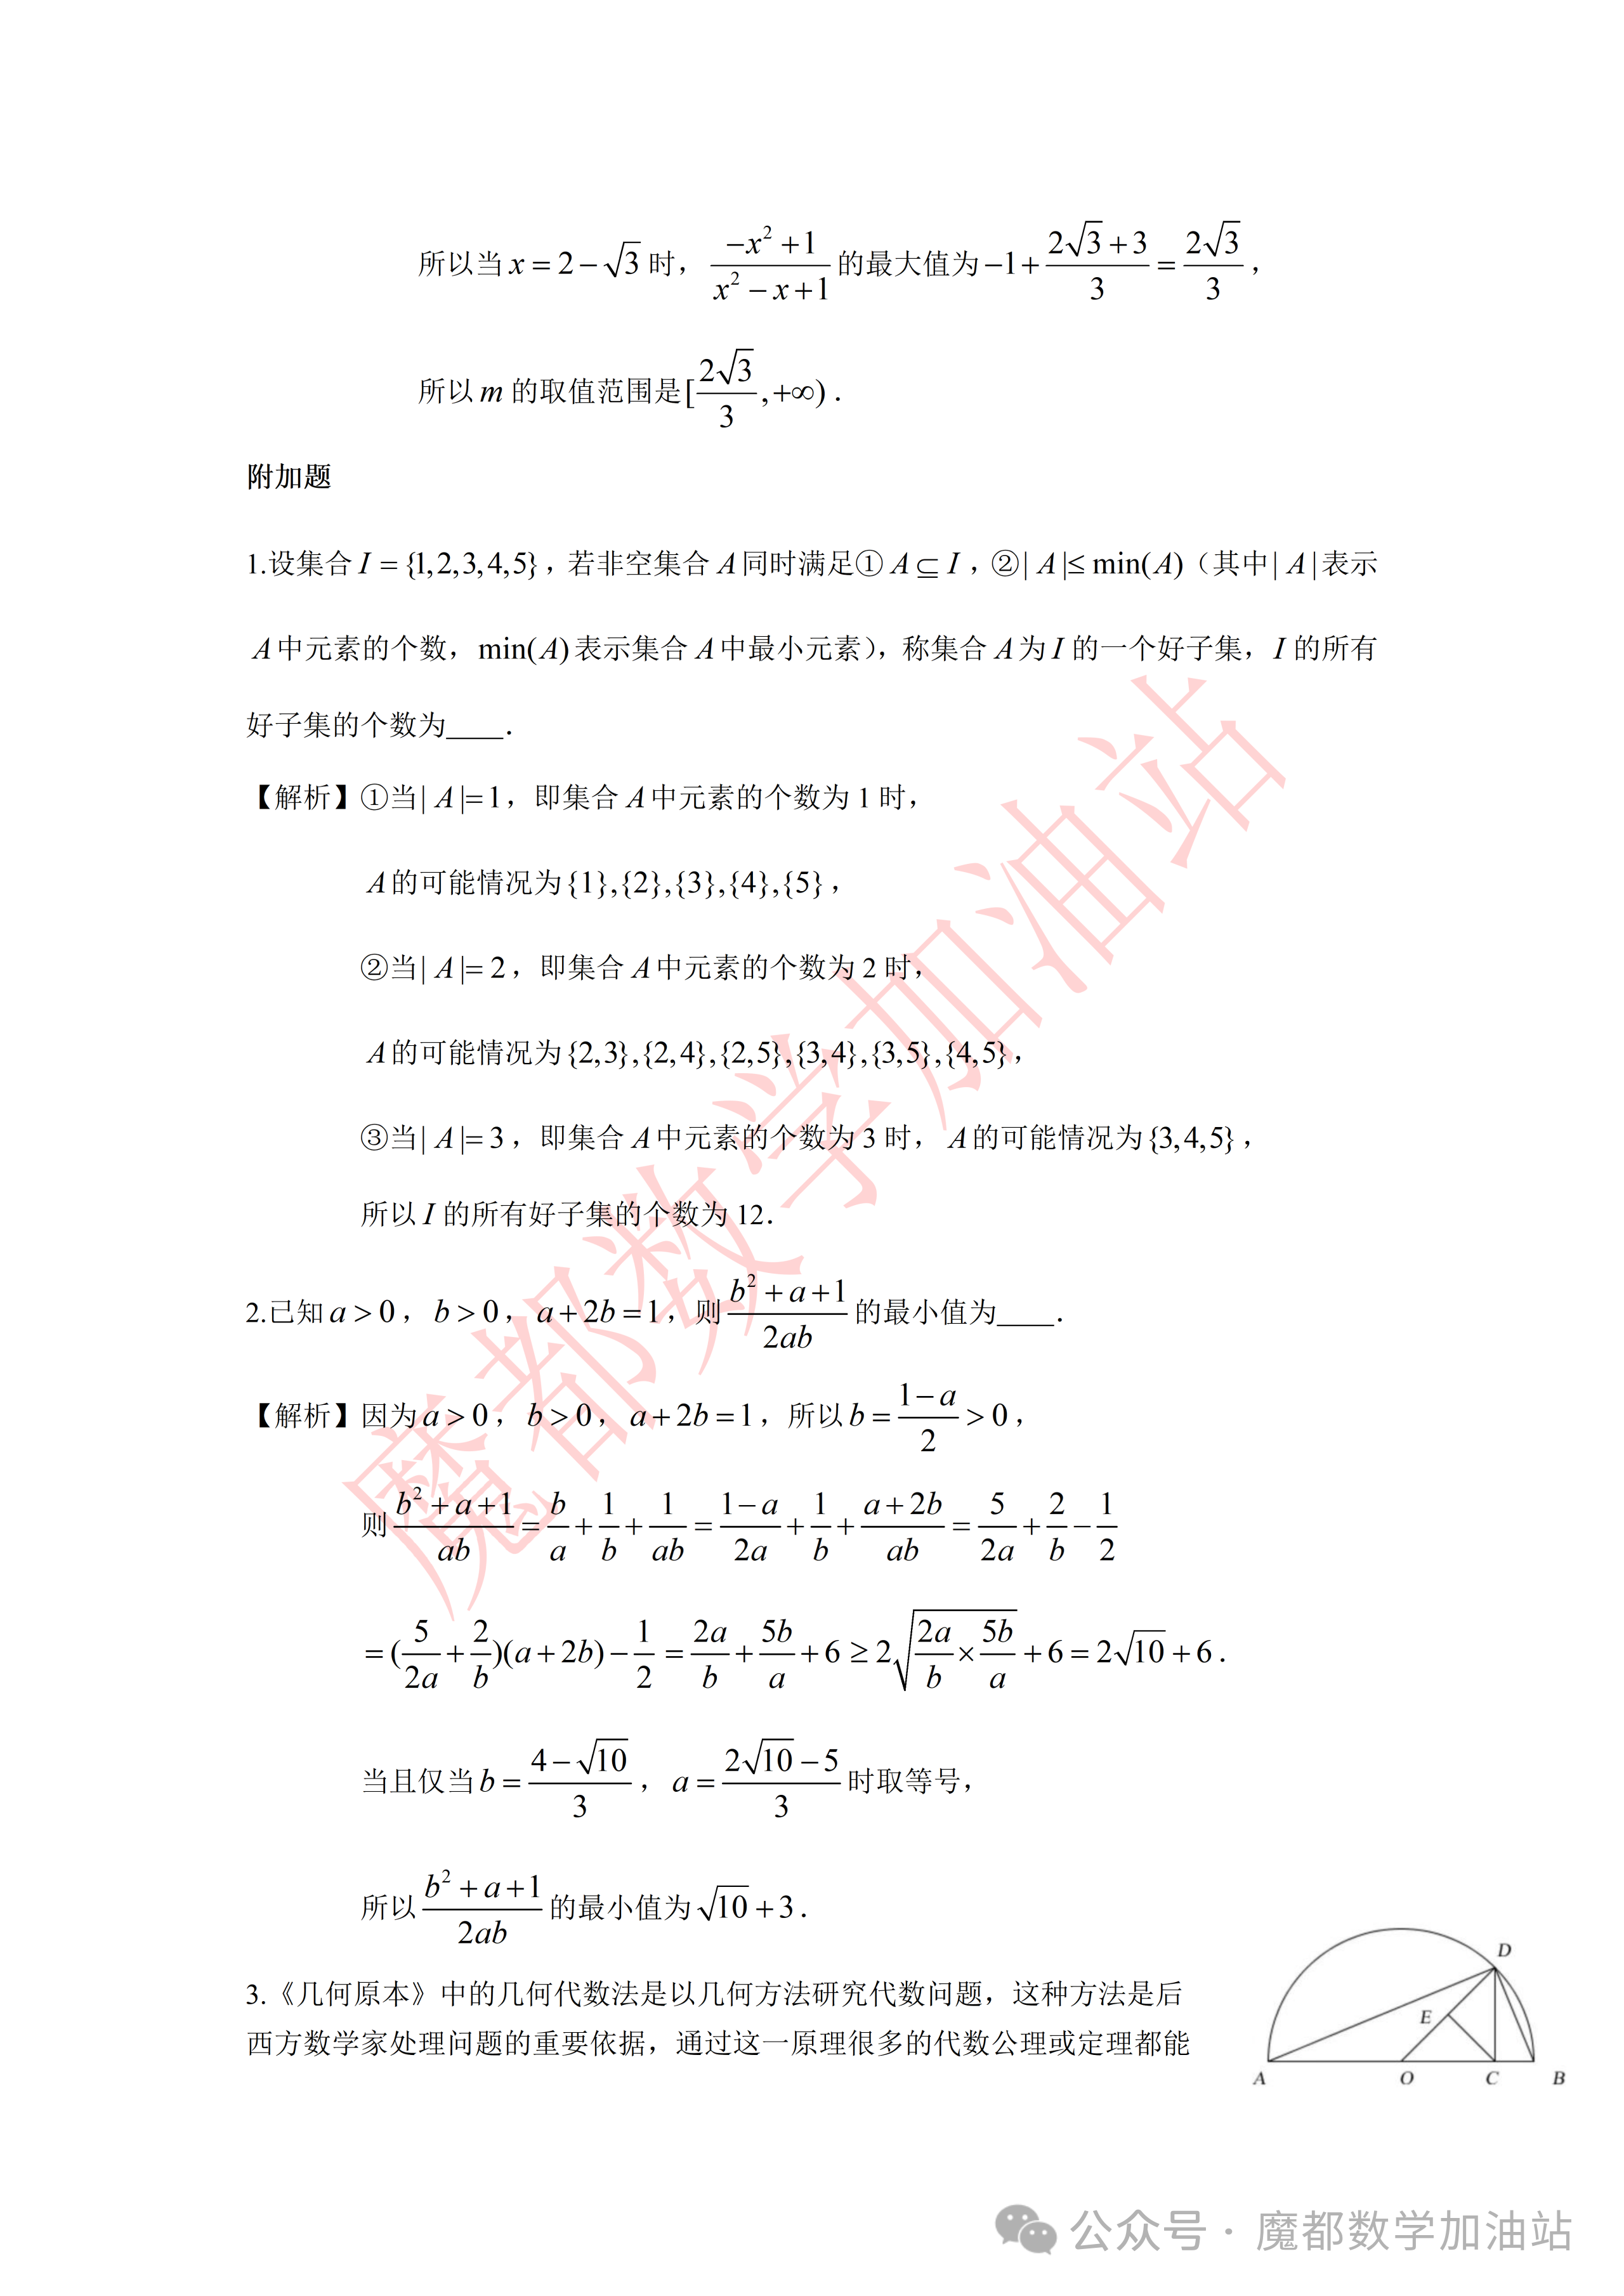
\includegraphics[width=.34\linewidth,trim=1960bp 310bp 90bp 3015bp,clip]{../原图/高一47_七宝中学_抱孩子练习9.26/08.png}
\end{center}

① $\dfrac{a+b}{2}\geqslant\sqrt{ab}$（$a>0$，$b>0$）；
② $a^2+b^2\geqslant2ab$（$a>0$，$b>0$）；
③ $\sqrt{ab}\geqslant\dfrac{2}{\dfrac1a+\dfrac1b}$（$a>0$，$b>0$）；
④ $\sqrt{\dfrac{a^2+b^2}{2}}\geqslant\dfrac{a+b}{2}$（$a>0$，$b>0$）.

\ifanswer
\solbegin
\step{因为 $AC+CB=a+b$，所以 $OD=\dfrac{AB}{2}=\dfrac{AC+CB}{2}=\dfrac{a+b}{2}$；}
\step{由射影定理得 $CD=\sqrt{AC\times CB}=\sqrt{ab}$，又因为 $OD\geqslant CD$，}
\step{所以 $\dfrac{a+b}{2}\geqslant\sqrt{ab}$，故①正确；}
\step{由射影定理得 $CD^2=DE\times OD$，所以 $DE=\dfrac{CD^2}{OD}=\dfrac{ab}{\dfrac{a+b}{2}}=\dfrac{2}{\dfrac1a+\dfrac1b}$，}
\step{又因为 $CD\geqslant DE$，所以 $\sqrt{ab}\geqslant\dfrac{2}{\dfrac1a+\dfrac1b}$，故③正确；}
\step{故该图形可以完成的所有无字证明为①③.}
\solend

\fi

% 注：原卷此处印作等式 $|x^2+a|+|x-a|=|x^2+x|$（在 $x>0$ 时与三角不等式下界等价），本稿曾改写成
% 不等式，现按原卷照录（原卷如此，照录未改）。
\item 若对任意 $x\in[2,3]$，均有 $|x^2+a|+|x-a|=|x^2+x|$，则实数 $a$ 的取值范围为 \blankline[4.4em].

\ifanswer
\solbegin
\step{因为 $|a|+|b|=|a+b|$ 当且仅当 $ab\geqslant0$ 时取等号，}
\step{所以 $(x^2+a)(x-a)\geqslant0$，即 $(a+x^2)(a-x)\leqslant0$，所以 $-x^2\leqslant a\leqslant x$ 恒成立，}
\step{因为 $x\in[2,3]$，所以 $-4\leqslant a\leqslant2$，所以实数 $a$ 的取值范围为 $[-4,2]$.}
\solend

\fi

\end{enumerate}

\end{document}
"
% 紧凑版：xelatex "\def\iscompact{1}% 高一47_七宝中学_抱孩子练习9.26.tex
%   —— 高一上数学“2026-2027 年七宝中学高一上抱孩子练习 9.26”（试卷版/答案版）
% 试卷版：xelatex 高一47_七宝中学_抱孩子练习9.26.tex
% 答案版：xelatex "\def\isanswer{1}\input{高一47_七宝中学_抱孩子练习9.26.tex}"
% 紧凑版：xelatex "\def\iscompact{1}\input{高一47_七宝中学_抱孩子练习9.26.tex}"
%
% 原始材料是微信公众号图文（公众号“魔都数学加油站”连载“27学年高一47”，署名“破晓”，
% 2026-10-02 17:56 发布，原文标题“27学年高一47——2026-2027年上海市七宝中学高一上抱孩子练习9.26”，
% 原文链接 https://mp.weixin.qq.com/s/mhkyDwjn7QFP_Z_NOcPkQA），正文为 9 张 PNG 页。
% 第 1—7、9 页分辨率为 4762×6735，第 8 页为 2560×3620；均按原图逐页核对。
% 原卷文字、选项、答案与解析均照录；粉色斜水印及灰色公众号页脚属水印/页脚，未录入。
%
% 卷首标题：原卷印作“2026-2027 年七宝中学高一上抱孩子练习 9.26”（公众号标题里的“上海市”
% 三字卷面标题行没有，本稿照卷面），年份区间按全稿惯例排 en dash，作业名保留原卷日期“9.26”。
% 原卷未印独立副标题；本稿按“知识模块”口径补出“集合与常用逻辑用语、不等式”。
%
% 与原卷的排版差异：
%   ① 原卷分“一、填空题”“二、选择题”“三、解答题”“附加题”四节；前三节题号为 3—16，
%      分别有 8 道填空、3 道选择、3 道解答；附加题另起 1—4 编号；
%   ② 原卷题下直接印答案/解析，本稿按全稿统一收进答案版；填空横线采用统一长度；
%   ③ 原卷未印副标题，本稿按“知识模块”口径补出（见卷首标题）；
%   ④ 全卷只有附加题第 3 题带图，直接从原卷第 8 页裁取。
%
% 原卷存疑（照录未改，见源码中该处上方注释）：
%   ① 第 9 题集合 C 的条件原文作“C={x|y=..., x 是整数}”，其中 y 未在集合描述中定义；
%      本稿照录原记号，未代换为 x。
%   ② 附加题第 3 题原文作“后西方数学家”，措辞存疑（疑漏“世”字）；本稿照录未改。
%
\documentclass[a4paper,11pt]{article}
\usepackage{common}

\begin{document}

\examtitlest[3]{2026--2027 年七宝中学高一上抱孩子练习 9.26}{集合与常用逻辑用语、不等式}

\bigsec{一、填空题}

\begin{enumerate}
\setcounter{enumi}{2}

\item 若不等式 $|x|<a$ 的一个充分条件为 $0<x<1$，则实数 $a$ 的取值范围是 \blankline[4.4em].

\ifanswer
\solbegin
\step{由 $|x|<a$ 得到 $-a<x<a$，}
\step{又不等式 $|x|<a$ 的一个充分条件为 $0<x<1$，所以 $a\geqslant1$.}
\solend

\fi

\item 已知命题“$\exists x\in\R$，使 $4x^2+(a-2)x+\dfrac14=0$”是假命题，则实数 $a$ 的取值范围是 \blankline[4.4em].

\ifanswer
\solbegin
% 注：原卷首句作“为真命题”（先按命题为真推出 $\Delta\geqslant0$，再由其为假得 $0<a<4$），原卷如此，照录未改。
\step{命题 $\exists x\in\R$，使 $4x^2+(a-2)x+\dfrac14=0$ 为真命题，}
\step{则 $\Delta=(a-2)^2-4\times4\times\dfrac14=a^2-4a\geqslant0$，解得 $a\leqslant0$ 或 $a\geqslant4$，}
\step{而命题“$\exists x\in\R$，使 $4x^2+(a-2)x+\dfrac14=0$”是假命题，则 $0<a<4$，}
\step{所以实数 $a$ 的取值范围是 $\{a\mid0<a<4\}$.}
\solend

\fi

\item 已知集合 $A=\{x\mid(a-1)x^2+3x-2=0\}$ 有且仅有两个子集，则实数 $a=$ \blankline[4.4em].

\ifanswer
\solbegin
\step{集合 $A=\{x\mid(a-1)x^2+3x-2=0\}$ 有且仅有两个不同的子集，}
\step{所以 $a-1=0$ 或 $\begin{cases}a-1\neq0\\\Delta=9+8(a-1)=0\end{cases}$，解得实数 $a=1$ 或 $a=-\dfrac18$.}
\solend

\fi

\item 已知函数 $y=x^2+bx+3$（其中 $b$ 是实数）中，$y$ 的取值范围是 $[0,+\infty)$，若关于 $x$ 的不等式 $x^2+bx+3<c$ 的解集为 $m-8<x<m$，则实数 $c$ 的值为 \blankline[4.4em].

\ifanswer
\solbegin
\step{因为 $y$ 的取值范围是 $[0,+\infty)$，所以 $\Delta=b^2-12=0$，解得 $b^2=12$，}
\step{因为不等式 $x^2+bx+3<c$ 的解集为 $m-8<x<m$，}
\step{令 $x^2+bx+3=c$，即 $x^2+bx+3-c=0$，方程的两根为 $x_1=m-8$，$x_2=m$，}
\step{所以 $|x_2-x_1|=\sqrt{(x_1+x_2)^2-4x_1x_2}=\sqrt{b^2-4(3-c)}=8$，即 $\sqrt{12-4(3-c)}=8$，}
\step{且判别式 $\Delta=b^2-4(3-c)=12-4(3-c)>0$，解得 $c=16$.}
\solend

\fi

\item 关于 $x$ 的不等式 $|x-1|+|x+1|\geqslant a$ 的解集为 $\R$，则实数 $a$ 的取值范围为 \blankline[4.4em].

\ifanswer
\solbegin
\step{因为 $|x-1|+|x+1|\geqslant|x-1-(x+1)|=2$，}
\step{若关于 $x$ 的不等式 $|x-1|+|x+1|\geqslant a$ 的解集为 $\R$，则实数 $a$ 的取值范围为 $a\leqslant2$.}
\solend

\fi

\item 已知 $m>0$，$xy>0$，当 $x+y=2$ 时，不等式 $\dfrac2x+\dfrac my\geqslant4$ 恒成立，则 $m$ 的取值范围是 \blankline[4.4em].

\ifanswer
\solbegin
\step{因为 $m>0$，$xy>0$，$x+y=2$，}
\step{所以 $\dfrac2x+\dfrac my=\dfrac12(x+y)\left(\dfrac2x+\dfrac my\right)
=\dfrac12\left(m+2+\dfrac{2y}{x}+\dfrac{mx}{y}\right)$}
\step{$\geqslant\dfrac12\left(m+2+2\sqrt{\dfrac{2y}{x}\cdot\dfrac{mx}{y}}\right)=\dfrac12\left(m+2+2\sqrt{2m}\right)$，}
\step{当且仅当 $\dfrac{2y}{x}=\dfrac{mx}{y}$，即 $y^2=\dfrac{mx^2}{2}$ 时取等号.}
\step{因为不等式 $\dfrac2x+\dfrac my\geqslant4$ 恒成立，所以 $\dfrac12(m+2+2\sqrt{2m})\geqslant4$，}
\step{整理得 $(\sqrt m+3\sqrt2)(\sqrt m-\sqrt2)\geqslant0$，解得 $\sqrt m\geqslant\sqrt2$，即 $m\geqslant2$，}
\step{所以 $m$ 的取值范围为 $[2,+\infty)$.}
\solend

\fi

\item 已知全集为 $\R$，集合 $D=\{x\mid x^2-ax+a^2-19=0\}$，
$B=\{y\mid y=-x^2+2x+2,\ y\text{ 是正整数}\}$，
% 注：本题集合 C 的条件原文作“C={x|y=..., x 是整数}”，其中 y 未在集合描述中定义；照录未改。
集合 $C=\left\{x\mathrel{\Big|}y=\sqrt{\dfrac{2-x}{x+1}},\ x\text{ 是整数}\right\}$，且集合 $D$ 满足 $D\cap B\neq\varnothing$，$\overline{D}\cup\overline{C}=\R$，则实数 $a$ 的值是 \blankline[4.4em].

\ifanswer
\solbegin
\step{集合 $B=\{y\mid y=-x^2+2x+2,\ y\text{ 是正整数}\}=\{1,2,3\}$，}
\step{集合 $C=\left\{x\mathrel{\Big|}y=\sqrt{\dfrac{2-x}{x+1}},\ x\text{ 是整数}\right\}=\{0,1,2\}$，}
\step{集合 $D=\{x\mid x^2-ax+a^2-19=0\}$ 且集合 $D$ 满足 $D\cap B\neq\varnothing$，$\overline{D}\cup\overline{C}=\R$，}
\step{所以 $3\in D$，解得 $a=5$ 或 $a=-2$，}
\step{经检验，$a=5$ 不符合 $\overline{D}\cup\overline{C}=\R$，舍去，$a=-2$ 满足题意，即 $a=-2$.}
\solend

\fi

% 注：本题解析中，$a=\pm2\sqrt2$ 时 $B$ 的二重根按 $-\dfrac a2$ 应为 $\mp\sqrt2$，原卷印作 $\mp2\sqrt2$、
% $-\dfrac{3\sqrt2}4$，$C(B)=3$ 的计算也随之按原卷保留（原卷如此，照录未改）。
\item 用 $C(A)$ 表示非空集合 $A$ 中的元素的个数，定义 $A*B=|C(A)-C(B)|$，已知集合 $A$ 有三个真子集，
$B=\{x\mid(ax^2+3x)(x^2+ax+2)=0,\ x\in\R\}$，若 $A*B=1$，设实数 $a$ 所有可能取值构成集合 $S$，则 $C(S)=$ \blankline[4.4em].

\ifanswer
\solbegin
\step{集合 $A$ 有三个真子集，则集合 $A$ 中有 $2$ 个元素，则 $C(A)=2$，}
\step{由 $A*B=1$，得 $C(B)=1$ 或 $3$，}
\step{即方程 $(ax^2+3x)\cdot(x^2+ax+2)=0$ 有一个根或 $3$ 个根；}
\step{若 $(ax^2+3x)\cdot(x^2+ax+2)=0$，则必有 $ax^2+3x=0$ 或 $x^2+ax+2=0$，}
\step{若 $ax^2+3x=0$，则 $x=0$ 或 $ax+3=0$，}
\step{当 $a=0$ 时，$B=\{0\}$，$C(B)=1$，符合题意；}
\step{当 $a\neq0$ 时，$ax^2+3x=0$ 对应的根为 $0$ 和 $-\dfrac3a$；}
\step{故①需 $x^2+ax+2=0$ 有两等根且根不为 $0$ 和 $-\dfrac3a$，}
\step{当 $\Delta=0$ 时，$a=\pm2\sqrt2$，}
\step{$a=2\sqrt2$，此时 $B=\left\{0,-2\sqrt2,-\dfrac{3\sqrt2}{4}\right\}$，$C(B)=3$，符合题意；}
\step{$a=-2\sqrt2$，此时 $B=\left\{0,2\sqrt2,\dfrac{3\sqrt2}{4}\right\}$，$C(B)=3$，符合题意；}
\step{②当 $-\dfrac3a$ 是 $x^2+ax+2=0$ 的根时，解得 $a=\pm3$；}
\step{$a=3$，此时 $B=\{0,-1,-2\}$，$C(B)=3$，符合题意；}
\step{$a=-3$，此时 $B=\{0,1,2\}$，$C(B)=3$，符合题意；}
\step{综上，$a$ 可取的值为 $0$、$\pm3$、$\pm2\sqrt2$，则 $C(S)=5$.}
\solend

\fi

\end{enumerate}

\bigsec{二、选择题}

\begin{enumerate}
\setcounter{enumi}{10}

\item 已知集合 $A=\left\{x\mathrel{\Big|}\dfrac1x<1\right\}$，$B=\{x\mid x^2-2x-3\leqslant0\}$，则 $A\cap B=$\mbox{（\quad）}

\keepwithprev
A. $\{x\mid1<x\leqslant3\}$\qquad B. $\{x\mid1\leqslant x\leqslant3\text{ 或 }-1\leqslant x<0\}$

C. $\{x\mid-1\leqslant x<0\}$\qquad D. $\{x\mid1<x\leqslant3\text{ 或 }-1\leqslant x<0\}$

\ans{$D$}

% 注：原卷本题只有题干＋选项（答案印在括号内），没有解析；此处照录原卷的"无解析"状态，不排解析。
\item 使 $x(y-2)=0$ 成立的一个充分条件是\mbox{（\quad）}

\keepwithprev
A. $x^2+(y-2)^2=0$\qquad B. $(x-2)^2+y^2=0$

C. $x^2+y^2=1$\qquad D. $x+y-2=0$

\ans{$A$}

\ifanswer
\solbegin
\step{对于 $A$：若 $x^2+(y-2)^2=0$，则 $x=0$ 且 $y=2$，此时 $x(y-2)=0$ 成立，}
\step{即充分性成立.}
\step{若 $x(y-2)=0$，则 $x=0$ 或 $y=2$，当 $x=0$，$y=3$ 时，$x^2+(y-2)^2=0$ 不成立，}
\step{即必要性不成立，}
\step{故 $x^2+(y-2)^2=0$ 是 $x(y-2)=0$ 成立的充分不必要条件；}
\step{对于 $B$：$(x-2)^2+y^2=0$，则 $x=2$ 且 $y=0$，此时 $x(y-2)=0$ 不成立，}
\step{即充分性不成立；}
\step{对于 $C$：$x^2+y^2=1$，此时 $x(y-2)=0$ 不一定成立，即充分性不成立；}
\step{对于 $D$：$x+y-2=0$，此时 $x(y-2)=0$ 不一定成立，即充分性不成立.}
\step{故选 $A$.}
\solend

\fi

\item 已知 $a$、$b$、$c\in\R$，若关于 $x$ 的不等式 $0\leqslant x+\dfrac ax+b\leqslant\dfrac cx-1$ 的解集为 $[x_1,x_2]\cup\{x_3\}$（$x_3>x_2>x_1>0$），则\mbox{（\quad）}

\keepwithprev
A. 不存在有序数组 $(a,b,c)$，使得 $x_2-x_1=1$

B. 存在唯一有序数组 $(a,b,c)$，使得 $x_2-x_1=1$

C. 有且只有两组有序数组 $(a,b,c)$，使得 $x_2-x_1=1$

D. 存在无穷多组有序数组 $(a,b,c)$，使得 $x_2-x_1=1$

\ans{$D$}

\ifanswer
\solbegin
\step{因为不等式 $0\leqslant x+\dfrac ax+b\leqslant\dfrac cx-1$ 的解集为 $[x_1,x_2]\cup\{x_3\}$（$x_3>x_2>x_1>0$），}
\step{所以 $0\leqslant x^2+bx+a\leqslant c-x$ 在 $[x_1,x_2]\cup\{x_3\}$ 上成立，}
\step{假设 $x_1=m$，$x_2=m+1$，$x_3=n$，}
\step{则 $c-n=0=n^2+bn+a$，由 $x_3$ 为一个独立的数得出，}
\step{所以 $n=c$，且 $m+1$ 与 $n$ 为方程 $x^2+bx+a=0$ 的两个根，}
\step{因为 $x_3>x_2>x_1>0$，所以 $-b=m+n+1=m+c+1$，$a=mn+n=mc+c$，}
\step{所以 $b=-m-c-1$，}
\step{且点 $(x_1,x_1^2+bx_1+a)$ 为 $y=x^2+bx+a$ 与 $y=c-x$ 的左交点，}
\step{所以 $m^2+bm+a=c-m$ 且 $b=-m-c-1$，$a=mc+c$，}
% 注：原卷此行的末句作“所以 $c-m=c-m$ 恒成立”（未写成 $x_2-x_1=1$），原卷如此，照录未改。
\step{故 $m^2+bm+a=m^2-m^2-mc-m+mc+c=c-m$，所以 $c-m=c-m$ 恒成立，}
\step{所以不论 $a$、$b$、$c$ 取何值，$x_2-x_1=1$ 恒成立，}
\step{即存在无穷多组有序数组 $(a,b,c)$，使得 $x_2-x_1=1$，}
\step{故选项 $A$、$B$、$C$ 错误，选项 $D$ 正确. 故选 $D$.}
\solend

\fi

\end{enumerate}

\bigsec{三、解答题}

\begin{enumerate}
\setcounter{enumi}{13}

\item 设正实数 $x$、$y$，满足 $2x+y=1$，求：

\begin{enumerate}[label=(\arabic*)]
\item $\sqrt{2x}+\sqrt y$ 的最大值；
\item $\dfrac2x+\dfrac1y$ 的最小值.
\end{enumerate}

\ifanswer
\solbegin
\stepm{(1)}{对于 $(\sqrt{2x}+\sqrt y)^2=2x+y+2\sqrt{2xy}\leqslant1+1=2$，}
\step{当且仅当 $\sqrt{2x}=\sqrt y$ 时取等号，故 $\sqrt{2x}+\sqrt y$ 的最大值为 $\sqrt2$；}
\stepm{(2)}{$\dfrac2x+\dfrac1y=\left(\dfrac2x+\dfrac1y\right)(2x+y)=5+\dfrac{2y}{x}+\dfrac{2x}{y}\geqslant5+4=9$，}
\step{当且仅当 $\dfrac{2y}{x}=\dfrac{2x}{y}$，即 $x=y=\dfrac13$ 时取等号，故 $\dfrac2x+\dfrac1y$ 的最小值为 $9$.}
\solend

\fi

\ansspace[6]

\item 设 $x_1$、$x_2$ 为关于 $x$ 的方程 $x^2-2(m+2)x+m^2-1=0$ 的两实数根.

\begin{enumerate}[label=(\arabic*)]
\item 若 $x_1$、$x_2$ 满足 $x_1^2+x_2^2=18$，试求 $m$ 的值；
\item 若 $x_1$、$x_2$ 均大于 $0$，求 $m$ 的取值范围.
\end{enumerate}

\ifanswer
\solbegin
\stepm{(1)}{由 $\Delta=4(m+2)^2-4(m^2-1)\geqslant0$，解得 $m\geqslant-\dfrac54$，}
\step{由韦达定理得 $x_1+x_2=2(m+2)$，$x_1x_2=m^2-1$，}
\step{又 $x_1^2+x_2^2=(x_1+x_2)^2-2x_1x_2=4(m+2)^2-2(m^2-1)=18$，}
\step{即 $m^2+8m=0$，解得 $m=0$ 或 $m=-8$（舍），故 $m$ 的值为 $0$；}
% 注：原卷此处作“由（2）得”（对照上一小问，所指应为（1）），原卷如此，照录未改。
\stepm{(2)}{由（2）得 $m\geqslant-\dfrac54$，}
\step{又 $x_1$、$x_2$ 均大于 $0$，则 $\begin{cases}2(m+2)>0\\m^2-1>0\end{cases}$，解得 $\begin{cases}m>-2\\m>1\text{或}m<-1\end{cases}$，}
\step{综上，实数 $m$ 的取值范围为 $\left[-\dfrac54,-1\right)\cup(1,+\infty)$.}
\solend

\fi

\ansspace[6]

\item 已知函数 $f(x)=(m+1)x^2-mx+m-1$（$m\in\R$）.

\begin{enumerate}[label=(\arabic*)]
\item 若不等式 $f(x)<0$ 的解集是空集，求 $m$ 的取值范围；
\item 当 $m>-2$ 时，解不等式 $f(x)\geqslant m$；
\item 若不等式 $f(x)\geqslant0$ 的解集为 $D$，若 $[-1,1]\subseteq D$，求 $m$ 的取值范围.
\end{enumerate}

\ifanswer
\solbegin
\stepm{(1)}{①当 $m+1=0$，即 $m=-1$ 时，$f(x)=x-2$，不合题意；}
\step{②当 $m+1\neq0$，即 $m\neq-1$ 时，$\begin{cases}m+1>0\\\Delta=m^2-4(m+1)(m-1)\leqslant0\end{cases}$，解得 $m\geqslant\dfrac{2\sqrt3}{3}$，}
\step{所以 $m$ 的取值范围是 $\left[\dfrac{2\sqrt3}{3},+\infty\right)$；}
\stepm{(2)}{因为 $f(x)\geqslant m$，所以 $(m+1)x^2-mx-1\geqslant0$，即 $[(m+1)x+1](x-1)\geqslant0$，}
\step{①当 $m+1=0$ 即 $m=-1$ 时，不等式的解集为 $[1,+\infty)$；}
\step{②当 $m+1>0$ 即 $m>-1$ 时，$\left(x+\dfrac1{m+1}\right)(x-1)\geqslant0$，}
\step{因为 $-\dfrac1{m+1}<0$，所以不等式的解集为 $\left(-\infty,-\dfrac1{m+1}\right]\cup[1,+\infty)$；}
\step{③当 $m+1<0$ 即 $-2<m<-1$ 时，$\left(x+\dfrac1{m+1}\right)(x-1)\leqslant0$，}
\step{因为 $-2<m<-1$，所以 $-1<m+1<0$，所以 $-\dfrac1{m+1}>1$，}
\step{所以不等式的解集为 $\left[1,-\dfrac1{m+1}\right]$；}
\stepm{(3)}{不等式 $f(x)\geqslant0$ 的解集为 $D$，若 $[-1,1]\subseteq D$，}
\step{即对任意的 $x\in[-1,1]$，不等式 $(m+1)x^2-mx+m-1\geqslant0$ 恒成立，}
\step{即 $m(x^2-x+1)\geqslant-x^2+1$ 恒成立，}
\step{因为 $x^2-x+1>0$ 恒成立，所以 $m\geqslant\dfrac{-x^2+1}{x^2-x+1}=-1+\dfrac{2-x}{x^2-x+1}$ 恒成立，}
\step{设 $t=2-x$，则 $t\in[1,3]$，$x=2-t$，}
\step{则 $\dfrac{2-x}{x^2-x+1}=\dfrac{t}{(2-t)^2-(2-t)+1}=\dfrac{t}{t^2-3t+3}=\dfrac1{t+\dfrac3t-3}$，}
\step{因为 $t+\dfrac3t\geqslant2\sqrt3$，当且仅当 $t=\sqrt3$ 时取等号，}
\step{所以 $\dfrac{2-x}{x^2-x+1}\leqslant\dfrac1{2\sqrt3-3}=\dfrac{2\sqrt3+3}{3}$，当且仅当 $x=2-\sqrt3$ 时取等号，}
\step{所以当 $x=2-\sqrt3$ 时，$\dfrac{-x^2+1}{x^2-x+1}$ 的最大值为 $-1+\dfrac{2\sqrt3+3}{3}=\dfrac{2\sqrt3}{3}$，}
\step{所以 $m$ 的取值范围是 $\left[\dfrac{2\sqrt3}{3},+\infty\right)$.}
\solend

\fi

\ansspace[8]

\end{enumerate}

\bigsec{附加题}

\begin{enumerate}

\item 设集合 $I=\{1,2,3,4,5\}$，若非空集合 $A$ 同时满足① $A\subseteq I$，② $|A|\leqslant\min(A)$（其中 $|A|$ 表示集合 $A$ 中元素的个数，$\min(A)$ 表示集合 $A$ 中最小元素），称集合 $A$ 为 $I$ 的一个好子集，$I$ 所有好子集的个数为 \blankline[4.4em].

\ifanswer
\solbegin
\step{①当 $|A|=1$，即集合 $A$ 中元素的个数为 $1$ 时，}
\step{$A$ 的可能情况为 $\{1\}$、$\{2\}$、$\{3\}$、$\{4\}$、$\{5\}$，}
\step{②当 $|A|=2$，即集合 $A$ 中元素的个数为 $2$ 时，}
\step{$A$ 的可能情况为 $\{2,3\}$、$\{2,4\}$、$\{2,5\}$、$\{3,4\}$、$\{3,5\}$、$\{4,5\}$，}
\step{③当 $|A|=3$，即集合 $A$ 中元素的个数为 $3$ 时，$A$ 的可能情况为 $\{3,4,5\}$，}
\step{所以 $I$ 的所有好子集的个数为 $12$.}
\solend

\fi

\item 已知 $a>0$，$b>0$，$a+2b=1$，则 $\dfrac{b^2+a+1}{2ab}$ 的最小值为 \blankline[4.4em].

\ifanswer
\solbegin
\step{因为 $a>0$，$b>0$，$a+2b=1$，所以 $b=\dfrac{1-a}{2}>0$，}
\step{则 $\dfrac{b^2+a+1}{ab}=\dfrac ba+\dfrac1b+\dfrac1{ab}=\dfrac{1-a}{2a}+\dfrac1b+\dfrac{a+2b}{ab}=\dfrac5{2a}+\dfrac2b-\dfrac12$}
\step{$=\left(\dfrac5{2a}+\dfrac2b\right)(a+2b)-\dfrac12=\dfrac{2a}{b}+\dfrac{5b}{a}+6\geqslant2\sqrt{\dfrac{2a}{b}\times\dfrac{5b}{a}}+6=2\sqrt{10}+6$.}
\step{当且仅当 $b=\dfrac{4-\sqrt{10}}{3}$，$a=\dfrac{2\sqrt{10}-5}{3}$ 时取等号，}
\step{所以 $\dfrac{b^2+a+1}{2ab}$ 的最小值为 $\sqrt{10}+3$.}
\solend

\fi

% 注：本题原文作“后西方数学家”，措辞存疑（疑漏“世”字）；照录未改，见文件头“原卷存疑”②。
% 又原文作"很多的代数公理或定理都能够通过图形实现证明"（"公理"疑为"公式"笔误）、
% "连结 OD,AD,BD"，均原卷如此，照录未改。
\item 《几何原本》中的几何代数法是以几何方法研究代数问题，这种方法是后西方数学家处理问题的重要依据，通过这一原理很多的代数公理或定理都能够通过图形实现证明，也称之为无字证明，现有图形如图所示，$C$ 为线段 $AB$ 上的点，且 $AC=a$，$BC=b$，$O$ 为 $AB$ 的中点，以 $AB$ 为直径作半圆，过点 $C$ 作 $AB$ 的垂线交半圆于 $D$，连结 $OD,AD,BD$，过点 $C$ 作 $OD$ 的垂线，垂足为 $E$，若不添加辅助线，则该图形可以完成的所有无字证明为 \blankline[4.4em]（填写序号）.

\begin{center}
% 插图直接裁自原卷第 8 页，未重绘；用 trim/clip 保留原图与标注。
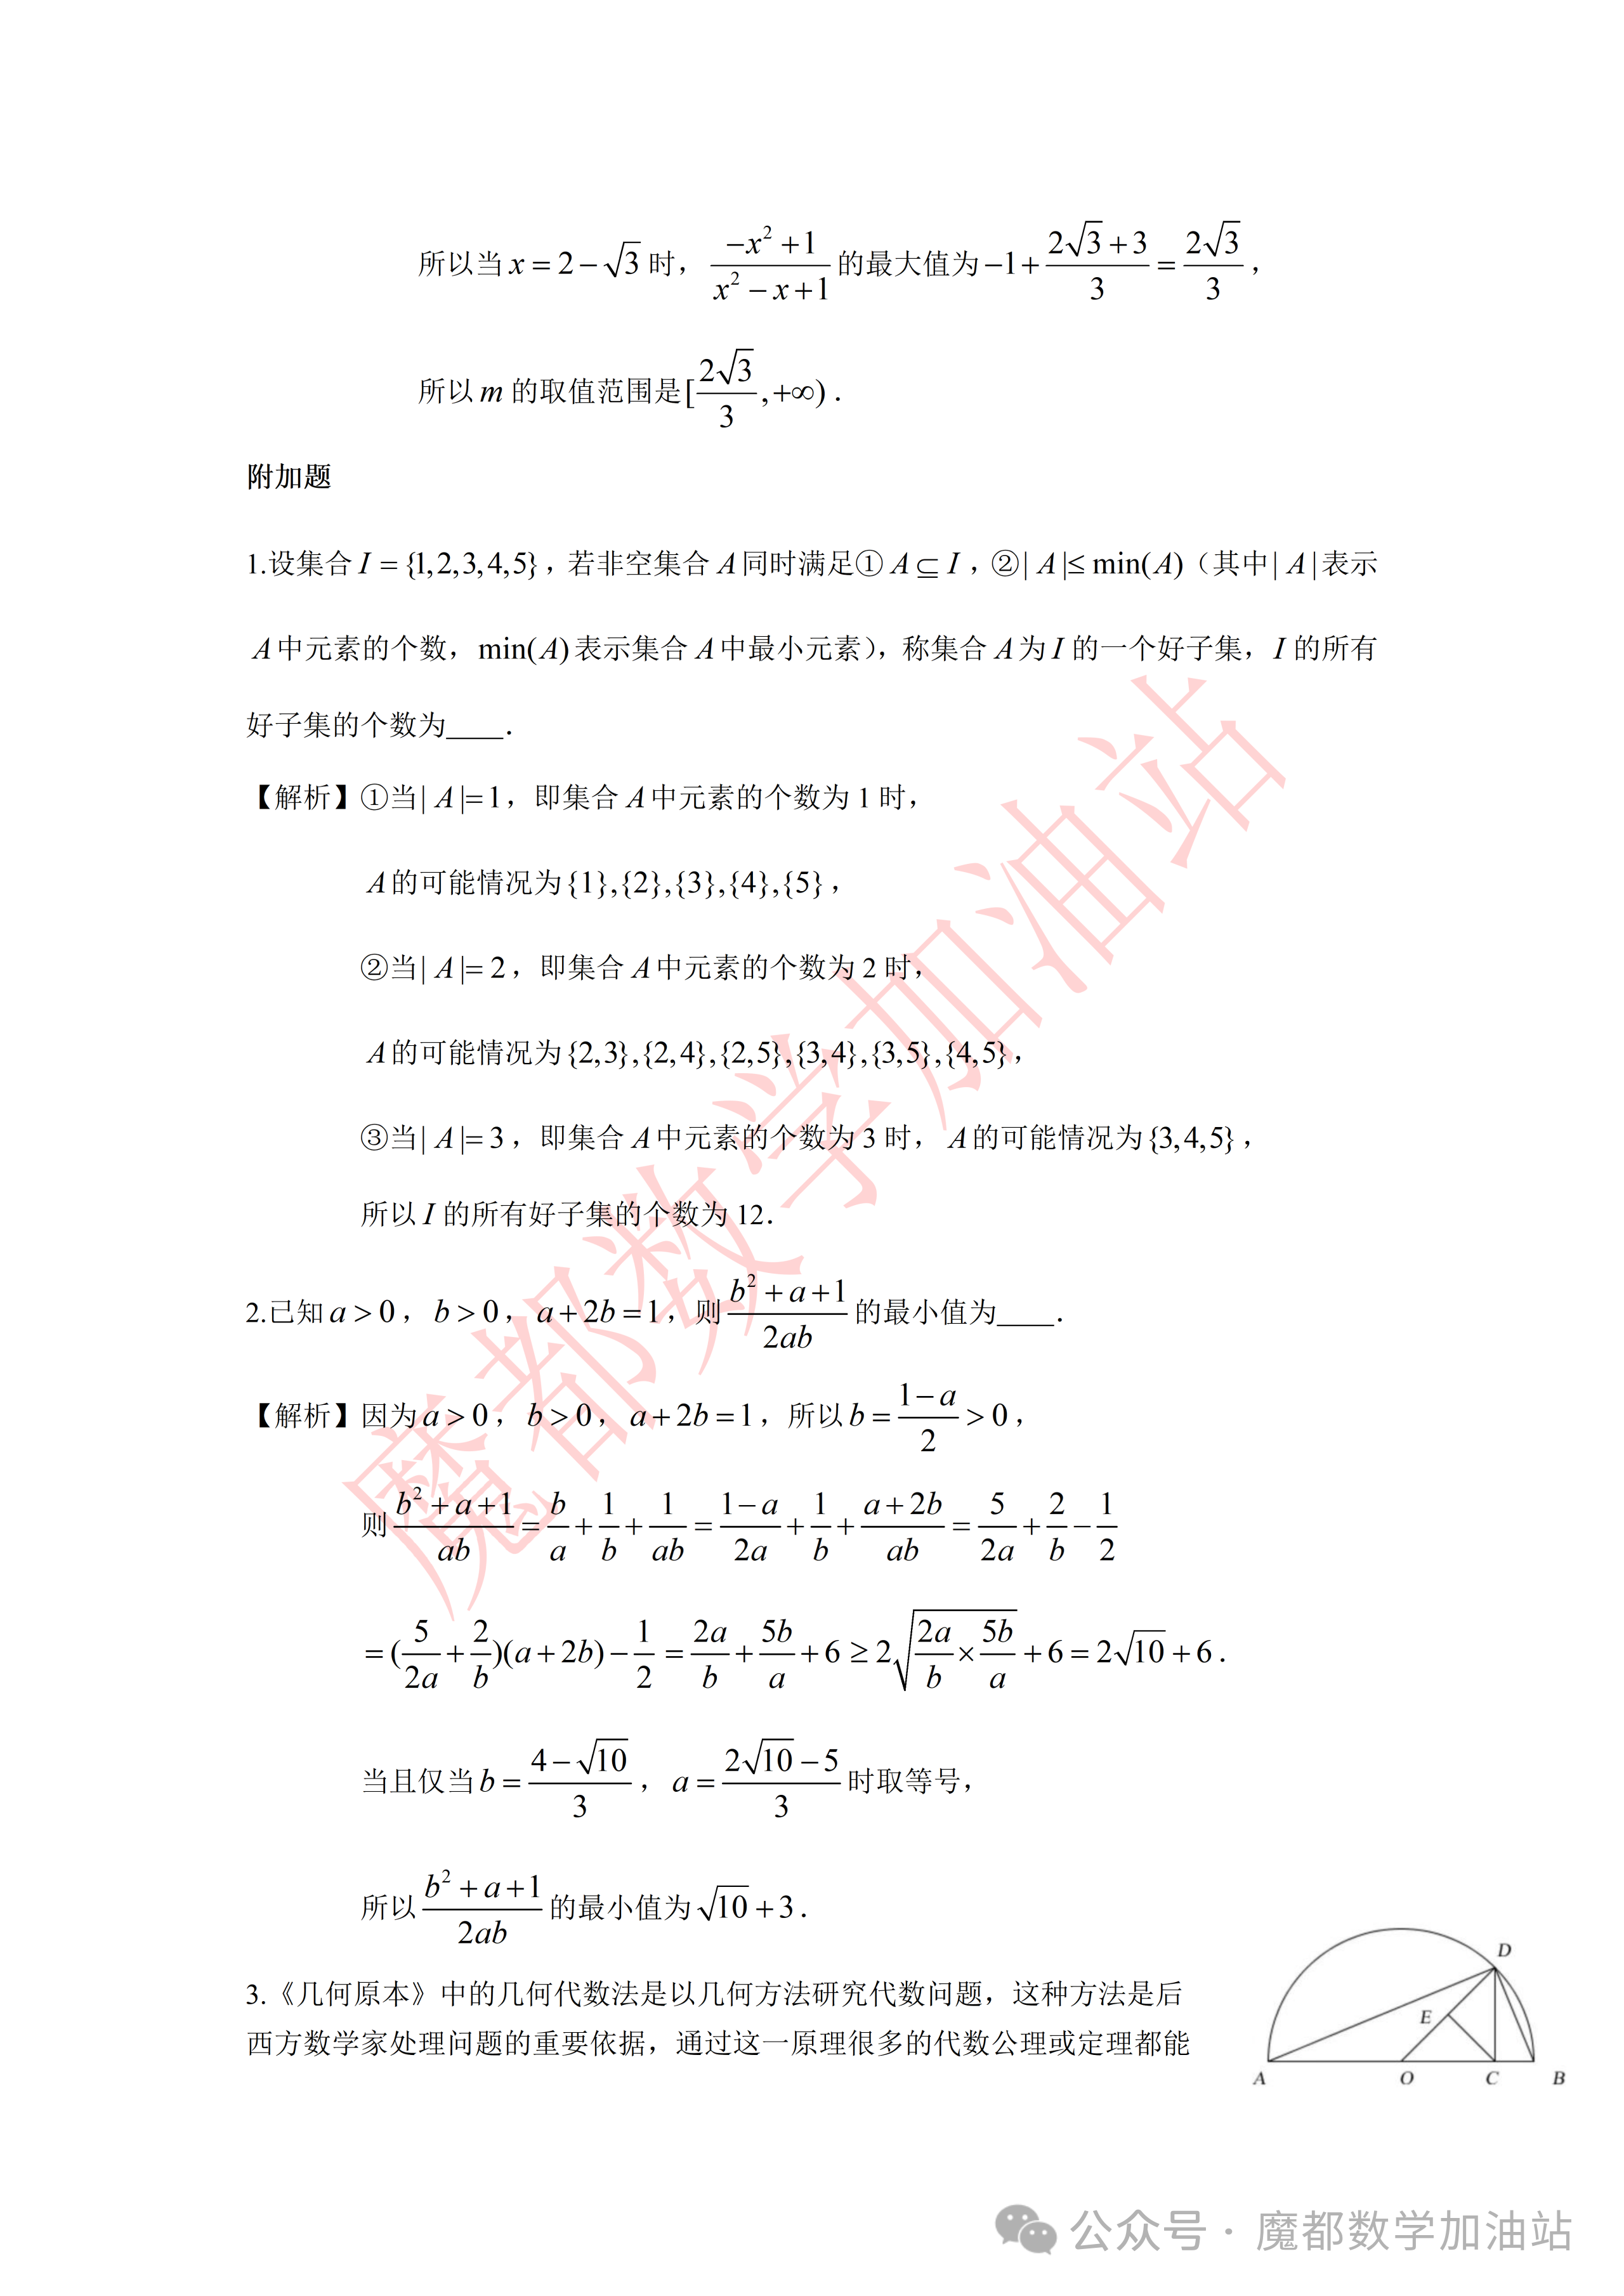
\includegraphics[width=.34\linewidth,trim=1960bp 310bp 90bp 3015bp,clip]{../原图/高一47_七宝中学_抱孩子练习9.26/08.png}
\end{center}

① $\dfrac{a+b}{2}\geqslant\sqrt{ab}$（$a>0$，$b>0$）；
② $a^2+b^2\geqslant2ab$（$a>0$，$b>0$）；
③ $\sqrt{ab}\geqslant\dfrac{2}{\dfrac1a+\dfrac1b}$（$a>0$，$b>0$）；
④ $\sqrt{\dfrac{a^2+b^2}{2}}\geqslant\dfrac{a+b}{2}$（$a>0$，$b>0$）.

\ifanswer
\solbegin
\step{因为 $AC+CB=a+b$，所以 $OD=\dfrac{AB}{2}=\dfrac{AC+CB}{2}=\dfrac{a+b}{2}$；}
\step{由射影定理得 $CD=\sqrt{AC\times CB}=\sqrt{ab}$，又因为 $OD\geqslant CD$，}
\step{所以 $\dfrac{a+b}{2}\geqslant\sqrt{ab}$，故①正确；}
\step{由射影定理得 $CD^2=DE\times OD$，所以 $DE=\dfrac{CD^2}{OD}=\dfrac{ab}{\dfrac{a+b}{2}}=\dfrac{2}{\dfrac1a+\dfrac1b}$，}
\step{又因为 $CD\geqslant DE$，所以 $\sqrt{ab}\geqslant\dfrac{2}{\dfrac1a+\dfrac1b}$，故③正确；}
\step{故该图形可以完成的所有无字证明为①③.}
\solend

\fi

% 注：原卷此处印作等式 $|x^2+a|+|x-a|=|x^2+x|$（在 $x>0$ 时与三角不等式下界等价），本稿曾改写成
% 不等式，现按原卷照录（原卷如此，照录未改）。
\item 若对任意 $x\in[2,3]$，均有 $|x^2+a|+|x-a|=|x^2+x|$，则实数 $a$ 的取值范围为 \blankline[4.4em].

\ifanswer
\solbegin
\step{因为 $|a|+|b|=|a+b|$ 当且仅当 $ab\geqslant0$ 时取等号，}
\step{所以 $(x^2+a)(x-a)\geqslant0$，即 $(a+x^2)(a-x)\leqslant0$，所以 $-x^2\leqslant a\leqslant x$ 恒成立，}
\step{因为 $x\in[2,3]$，所以 $-4\leqslant a\leqslant2$，所以实数 $a$ 的取值范围为 $[-4,2]$.}
\solend

\fi

\end{enumerate}

\end{document}
"
%
% 原始材料是微信公众号图文（公众号“魔都数学加油站”连载“27学年高一47”，署名“破晓”，
% 2026-10-02 17:56 发布，原文标题“27学年高一47——2026-2027年上海市七宝中学高一上抱孩子练习9.26”，
% 原文链接 https://mp.weixin.qq.com/s/mhkyDwjn7QFP_Z_NOcPkQA），正文为 9 张 PNG 页。
% 第 1—7、9 页分辨率为 4762×6735，第 8 页为 2560×3620；均按原图逐页核对。
% 原卷文字、选项、答案与解析均照录；粉色斜水印及灰色公众号页脚属水印/页脚，未录入。
%
% 卷首标题：原卷印作“2026-2027 年七宝中学高一上抱孩子练习 9.26”（公众号标题里的“上海市”
% 三字卷面标题行没有，本稿照卷面），年份区间按全稿惯例排 en dash，作业名保留原卷日期“9.26”。
% 原卷未印独立副标题；本稿按“知识模块”口径补出“集合与常用逻辑用语、不等式”。
%
% 与原卷的排版差异：
%   ① 原卷分“一、填空题”“二、选择题”“三、解答题”“附加题”四节；前三节题号为 3—16，
%      分别有 8 道填空、3 道选择、3 道解答；附加题另起 1—4 编号；
%   ② 原卷题下直接印答案/解析，本稿按全稿统一收进答案版；填空横线采用统一长度；
%   ③ 原卷未印副标题，本稿按“知识模块”口径补出（见卷首标题）；
%   ④ 全卷只有附加题第 3 题带图，直接从原卷第 8 页裁取。
%
% 原卷存疑（照录未改，见源码中该处上方注释）：
%   ① 第 9 题集合 C 的条件原文作“C={x|y=..., x 是整数}”，其中 y 未在集合描述中定义；
%      本稿照录原记号，未代换为 x。
%   ② 附加题第 3 题原文作“后西方数学家”，措辞存疑（疑漏“世”字）；本稿照录未改。
%
\documentclass[a4paper,11pt]{article}
\usepackage{common}

\begin{document}

\examtitlest[3]{2026--2027 年七宝中学高一上抱孩子练习 9.26}{集合与常用逻辑用语、不等式}

\bigsec{一、填空题}

\begin{enumerate}
\setcounter{enumi}{2}

\item 若不等式 $|x|<a$ 的一个充分条件为 $0<x<1$，则实数 $a$ 的取值范围是 \blankline[4.4em].

\ifanswer
\solbegin
\step{由 $|x|<a$ 得到 $-a<x<a$，}
\step{又不等式 $|x|<a$ 的一个充分条件为 $0<x<1$，所以 $a\geqslant1$.}
\solend

\fi

\item 已知命题“$\exists x\in\R$，使 $4x^2+(a-2)x+\dfrac14=0$”是假命题，则实数 $a$ 的取值范围是 \blankline[4.4em].

\ifanswer
\solbegin
% 注：原卷首句作“为真命题”（先按命题为真推出 $\Delta\geqslant0$，再由其为假得 $0<a<4$），原卷如此，照录未改。
\step{命题 $\exists x\in\R$，使 $4x^2+(a-2)x+\dfrac14=0$ 为真命题，}
\step{则 $\Delta=(a-2)^2-4\times4\times\dfrac14=a^2-4a\geqslant0$，解得 $a\leqslant0$ 或 $a\geqslant4$，}
\step{而命题“$\exists x\in\R$，使 $4x^2+(a-2)x+\dfrac14=0$”是假命题，则 $0<a<4$，}
\step{所以实数 $a$ 的取值范围是 $\{a\mid0<a<4\}$.}
\solend

\fi

\item 已知集合 $A=\{x\mid(a-1)x^2+3x-2=0\}$ 有且仅有两个子集，则实数 $a=$ \blankline[4.4em].

\ifanswer
\solbegin
\step{集合 $A=\{x\mid(a-1)x^2+3x-2=0\}$ 有且仅有两个不同的子集，}
\step{所以 $a-1=0$ 或 $\begin{cases}a-1\neq0\\\Delta=9+8(a-1)=0\end{cases}$，解得实数 $a=1$ 或 $a=-\dfrac18$.}
\solend

\fi

\item 已知函数 $y=x^2+bx+3$（其中 $b$ 是实数）中，$y$ 的取值范围是 $[0,+\infty)$，若关于 $x$ 的不等式 $x^2+bx+3<c$ 的解集为 $m-8<x<m$，则实数 $c$ 的值为 \blankline[4.4em].

\ifanswer
\solbegin
\step{因为 $y$ 的取值范围是 $[0,+\infty)$，所以 $\Delta=b^2-12=0$，解得 $b^2=12$，}
\step{因为不等式 $x^2+bx+3<c$ 的解集为 $m-8<x<m$，}
\step{令 $x^2+bx+3=c$，即 $x^2+bx+3-c=0$，方程的两根为 $x_1=m-8$，$x_2=m$，}
\step{所以 $|x_2-x_1|=\sqrt{(x_1+x_2)^2-4x_1x_2}=\sqrt{b^2-4(3-c)}=8$，即 $\sqrt{12-4(3-c)}=8$，}
\step{且判别式 $\Delta=b^2-4(3-c)=12-4(3-c)>0$，解得 $c=16$.}
\solend

\fi

\item 关于 $x$ 的不等式 $|x-1|+|x+1|\geqslant a$ 的解集为 $\R$，则实数 $a$ 的取值范围为 \blankline[4.4em].

\ifanswer
\solbegin
\step{因为 $|x-1|+|x+1|\geqslant|x-1-(x+1)|=2$，}
\step{若关于 $x$ 的不等式 $|x-1|+|x+1|\geqslant a$ 的解集为 $\R$，则实数 $a$ 的取值范围为 $a\leqslant2$.}
\solend

\fi

\item 已知 $m>0$，$xy>0$，当 $x+y=2$ 时，不等式 $\dfrac2x+\dfrac my\geqslant4$ 恒成立，则 $m$ 的取值范围是 \blankline[4.4em].

\ifanswer
\solbegin
\step{因为 $m>0$，$xy>0$，$x+y=2$，}
\step{所以 $\dfrac2x+\dfrac my=\dfrac12(x+y)\left(\dfrac2x+\dfrac my\right)
=\dfrac12\left(m+2+\dfrac{2y}{x}+\dfrac{mx}{y}\right)$}
\step{$\geqslant\dfrac12\left(m+2+2\sqrt{\dfrac{2y}{x}\cdot\dfrac{mx}{y}}\right)=\dfrac12\left(m+2+2\sqrt{2m}\right)$，}
\step{当且仅当 $\dfrac{2y}{x}=\dfrac{mx}{y}$，即 $y^2=\dfrac{mx^2}{2}$ 时取等号.}
\step{因为不等式 $\dfrac2x+\dfrac my\geqslant4$ 恒成立，所以 $\dfrac12(m+2+2\sqrt{2m})\geqslant4$，}
\step{整理得 $(\sqrt m+3\sqrt2)(\sqrt m-\sqrt2)\geqslant0$，解得 $\sqrt m\geqslant\sqrt2$，即 $m\geqslant2$，}
\step{所以 $m$ 的取值范围为 $[2,+\infty)$.}
\solend

\fi

\item 已知全集为 $\R$，集合 $D=\{x\mid x^2-ax+a^2-19=0\}$，
$B=\{y\mid y=-x^2+2x+2,\ y\text{ 是正整数}\}$，
% 注：本题集合 C 的条件原文作“C={x|y=..., x 是整数}”，其中 y 未在集合描述中定义；照录未改。
集合 $C=\left\{x\mathrel{\Big|}y=\sqrt{\dfrac{2-x}{x+1}},\ x\text{ 是整数}\right\}$，且集合 $D$ 满足 $D\cap B\neq\varnothing$，$\overline{D}\cup\overline{C}=\R$，则实数 $a$ 的值是 \blankline[4.4em].

\ifanswer
\solbegin
\step{集合 $B=\{y\mid y=-x^2+2x+2,\ y\text{ 是正整数}\}=\{1,2,3\}$，}
\step{集合 $C=\left\{x\mathrel{\Big|}y=\sqrt{\dfrac{2-x}{x+1}},\ x\text{ 是整数}\right\}=\{0,1,2\}$，}
\step{集合 $D=\{x\mid x^2-ax+a^2-19=0\}$ 且集合 $D$ 满足 $D\cap B\neq\varnothing$，$\overline{D}\cup\overline{C}=\R$，}
\step{所以 $3\in D$，解得 $a=5$ 或 $a=-2$，}
\step{经检验，$a=5$ 不符合 $\overline{D}\cup\overline{C}=\R$，舍去，$a=-2$ 满足题意，即 $a=-2$.}
\solend

\fi

% 注：本题解析中，$a=\pm2\sqrt2$ 时 $B$ 的二重根按 $-\dfrac a2$ 应为 $\mp\sqrt2$，原卷印作 $\mp2\sqrt2$、
% $-\dfrac{3\sqrt2}4$，$C(B)=3$ 的计算也随之按原卷保留（原卷如此，照录未改）。
\item 用 $C(A)$ 表示非空集合 $A$ 中的元素的个数，定义 $A*B=|C(A)-C(B)|$，已知集合 $A$ 有三个真子集，
$B=\{x\mid(ax^2+3x)(x^2+ax+2)=0,\ x\in\R\}$，若 $A*B=1$，设实数 $a$ 所有可能取值构成集合 $S$，则 $C(S)=$ \blankline[4.4em].

\ifanswer
\solbegin
\step{集合 $A$ 有三个真子集，则集合 $A$ 中有 $2$ 个元素，则 $C(A)=2$，}
\step{由 $A*B=1$，得 $C(B)=1$ 或 $3$，}
\step{即方程 $(ax^2+3x)\cdot(x^2+ax+2)=0$ 有一个根或 $3$ 个根；}
\step{若 $(ax^2+3x)\cdot(x^2+ax+2)=0$，则必有 $ax^2+3x=0$ 或 $x^2+ax+2=0$，}
\step{若 $ax^2+3x=0$，则 $x=0$ 或 $ax+3=0$，}
\step{当 $a=0$ 时，$B=\{0\}$，$C(B)=1$，符合题意；}
\step{当 $a\neq0$ 时，$ax^2+3x=0$ 对应的根为 $0$ 和 $-\dfrac3a$；}
\step{故①需 $x^2+ax+2=0$ 有两等根且根不为 $0$ 和 $-\dfrac3a$，}
\step{当 $\Delta=0$ 时，$a=\pm2\sqrt2$，}
\step{$a=2\sqrt2$，此时 $B=\left\{0,-2\sqrt2,-\dfrac{3\sqrt2}{4}\right\}$，$C(B)=3$，符合题意；}
\step{$a=-2\sqrt2$，此时 $B=\left\{0,2\sqrt2,\dfrac{3\sqrt2}{4}\right\}$，$C(B)=3$，符合题意；}
\step{②当 $-\dfrac3a$ 是 $x^2+ax+2=0$ 的根时，解得 $a=\pm3$；}
\step{$a=3$，此时 $B=\{0,-1,-2\}$，$C(B)=3$，符合题意；}
\step{$a=-3$，此时 $B=\{0,1,2\}$，$C(B)=3$，符合题意；}
\step{综上，$a$ 可取的值为 $0$、$\pm3$、$\pm2\sqrt2$，则 $C(S)=5$.}
\solend

\fi

\end{enumerate}

\bigsec{二、选择题}

\begin{enumerate}
\setcounter{enumi}{10}

\item 已知集合 $A=\left\{x\mathrel{\Big|}\dfrac1x<1\right\}$，$B=\{x\mid x^2-2x-3\leqslant0\}$，则 $A\cap B=$\mbox{（\quad）}

\keepwithprev
A. $\{x\mid1<x\leqslant3\}$\qquad B. $\{x\mid1\leqslant x\leqslant3\text{ 或 }-1\leqslant x<0\}$

C. $\{x\mid-1\leqslant x<0\}$\qquad D. $\{x\mid1<x\leqslant3\text{ 或 }-1\leqslant x<0\}$

\ans{$D$}

% 注：原卷本题只有题干＋选项（答案印在括号内），没有解析；此处照录原卷的"无解析"状态，不排解析。
\item 使 $x(y-2)=0$ 成立的一个充分条件是\mbox{（\quad）}

\keepwithprev
A. $x^2+(y-2)^2=0$\qquad B. $(x-2)^2+y^2=0$

C. $x^2+y^2=1$\qquad D. $x+y-2=0$

\ans{$A$}

\ifanswer
\solbegin
\step{对于 $A$：若 $x^2+(y-2)^2=0$，则 $x=0$ 且 $y=2$，此时 $x(y-2)=0$ 成立，}
\step{即充分性成立.}
\step{若 $x(y-2)=0$，则 $x=0$ 或 $y=2$，当 $x=0$，$y=3$ 时，$x^2+(y-2)^2=0$ 不成立，}
\step{即必要性不成立，}
\step{故 $x^2+(y-2)^2=0$ 是 $x(y-2)=0$ 成立的充分不必要条件；}
\step{对于 $B$：$(x-2)^2+y^2=0$，则 $x=2$ 且 $y=0$，此时 $x(y-2)=0$ 不成立，}
\step{即充分性不成立；}
\step{对于 $C$：$x^2+y^2=1$，此时 $x(y-2)=0$ 不一定成立，即充分性不成立；}
\step{对于 $D$：$x+y-2=0$，此时 $x(y-2)=0$ 不一定成立，即充分性不成立.}
\step{故选 $A$.}
\solend

\fi

\item 已知 $a$、$b$、$c\in\R$，若关于 $x$ 的不等式 $0\leqslant x+\dfrac ax+b\leqslant\dfrac cx-1$ 的解集为 $[x_1,x_2]\cup\{x_3\}$（$x_3>x_2>x_1>0$），则\mbox{（\quad）}

\keepwithprev
A. 不存在有序数组 $(a,b,c)$，使得 $x_2-x_1=1$

B. 存在唯一有序数组 $(a,b,c)$，使得 $x_2-x_1=1$

C. 有且只有两组有序数组 $(a,b,c)$，使得 $x_2-x_1=1$

D. 存在无穷多组有序数组 $(a,b,c)$，使得 $x_2-x_1=1$

\ans{$D$}

\ifanswer
\solbegin
\step{因为不等式 $0\leqslant x+\dfrac ax+b\leqslant\dfrac cx-1$ 的解集为 $[x_1,x_2]\cup\{x_3\}$（$x_3>x_2>x_1>0$），}
\step{所以 $0\leqslant x^2+bx+a\leqslant c-x$ 在 $[x_1,x_2]\cup\{x_3\}$ 上成立，}
\step{假设 $x_1=m$，$x_2=m+1$，$x_3=n$，}
\step{则 $c-n=0=n^2+bn+a$，由 $x_3$ 为一个独立的数得出，}
\step{所以 $n=c$，且 $m+1$ 与 $n$ 为方程 $x^2+bx+a=0$ 的两个根，}
\step{因为 $x_3>x_2>x_1>0$，所以 $-b=m+n+1=m+c+1$，$a=mn+n=mc+c$，}
\step{所以 $b=-m-c-1$，}
\step{且点 $(x_1,x_1^2+bx_1+a)$ 为 $y=x^2+bx+a$ 与 $y=c-x$ 的左交点，}
\step{所以 $m^2+bm+a=c-m$ 且 $b=-m-c-1$，$a=mc+c$，}
% 注：原卷此行的末句作“所以 $c-m=c-m$ 恒成立”（未写成 $x_2-x_1=1$），原卷如此，照录未改。
\step{故 $m^2+bm+a=m^2-m^2-mc-m+mc+c=c-m$，所以 $c-m=c-m$ 恒成立，}
\step{所以不论 $a$、$b$、$c$ 取何值，$x_2-x_1=1$ 恒成立，}
\step{即存在无穷多组有序数组 $(a,b,c)$，使得 $x_2-x_1=1$，}
\step{故选项 $A$、$B$、$C$ 错误，选项 $D$ 正确. 故选 $D$.}
\solend

\fi

\end{enumerate}

\bigsec{三、解答题}

\begin{enumerate}
\setcounter{enumi}{13}

\item 设正实数 $x$、$y$，满足 $2x+y=1$，求：

\begin{enumerate}[label=(\arabic*)]
\item $\sqrt{2x}+\sqrt y$ 的最大值；
\item $\dfrac2x+\dfrac1y$ 的最小值.
\end{enumerate}

\ifanswer
\solbegin
\stepm{(1)}{对于 $(\sqrt{2x}+\sqrt y)^2=2x+y+2\sqrt{2xy}\leqslant1+1=2$，}
\step{当且仅当 $\sqrt{2x}=\sqrt y$ 时取等号，故 $\sqrt{2x}+\sqrt y$ 的最大值为 $\sqrt2$；}
\stepm{(2)}{$\dfrac2x+\dfrac1y=\left(\dfrac2x+\dfrac1y\right)(2x+y)=5+\dfrac{2y}{x}+\dfrac{2x}{y}\geqslant5+4=9$，}
\step{当且仅当 $\dfrac{2y}{x}=\dfrac{2x}{y}$，即 $x=y=\dfrac13$ 时取等号，故 $\dfrac2x+\dfrac1y$ 的最小值为 $9$.}
\solend

\fi

\ansspace[6]

\item 设 $x_1$、$x_2$ 为关于 $x$ 的方程 $x^2-2(m+2)x+m^2-1=0$ 的两实数根.

\begin{enumerate}[label=(\arabic*)]
\item 若 $x_1$、$x_2$ 满足 $x_1^2+x_2^2=18$，试求 $m$ 的值；
\item 若 $x_1$、$x_2$ 均大于 $0$，求 $m$ 的取值范围.
\end{enumerate}

\ifanswer
\solbegin
\stepm{(1)}{由 $\Delta=4(m+2)^2-4(m^2-1)\geqslant0$，解得 $m\geqslant-\dfrac54$，}
\step{由韦达定理得 $x_1+x_2=2(m+2)$，$x_1x_2=m^2-1$，}
\step{又 $x_1^2+x_2^2=(x_1+x_2)^2-2x_1x_2=4(m+2)^2-2(m^2-1)=18$，}
\step{即 $m^2+8m=0$，解得 $m=0$ 或 $m=-8$（舍），故 $m$ 的值为 $0$；}
% 注：原卷此处作“由（2）得”（对照上一小问，所指应为（1）），原卷如此，照录未改。
\stepm{(2)}{由（2）得 $m\geqslant-\dfrac54$，}
\step{又 $x_1$、$x_2$ 均大于 $0$，则 $\begin{cases}2(m+2)>0\\m^2-1>0\end{cases}$，解得 $\begin{cases}m>-2\\m>1\text{或}m<-1\end{cases}$，}
\step{综上，实数 $m$ 的取值范围为 $\left[-\dfrac54,-1\right)\cup(1,+\infty)$.}
\solend

\fi

\ansspace[6]

\item 已知函数 $f(x)=(m+1)x^2-mx+m-1$（$m\in\R$）.

\begin{enumerate}[label=(\arabic*)]
\item 若不等式 $f(x)<0$ 的解集是空集，求 $m$ 的取值范围；
\item 当 $m>-2$ 时，解不等式 $f(x)\geqslant m$；
\item 若不等式 $f(x)\geqslant0$ 的解集为 $D$，若 $[-1,1]\subseteq D$，求 $m$ 的取值范围.
\end{enumerate}

\ifanswer
\solbegin
\stepm{(1)}{①当 $m+1=0$，即 $m=-1$ 时，$f(x)=x-2$，不合题意；}
\step{②当 $m+1\neq0$，即 $m\neq-1$ 时，$\begin{cases}m+1>0\\\Delta=m^2-4(m+1)(m-1)\leqslant0\end{cases}$，解得 $m\geqslant\dfrac{2\sqrt3}{3}$，}
\step{所以 $m$ 的取值范围是 $\left[\dfrac{2\sqrt3}{3},+\infty\right)$；}
\stepm{(2)}{因为 $f(x)\geqslant m$，所以 $(m+1)x^2-mx-1\geqslant0$，即 $[(m+1)x+1](x-1)\geqslant0$，}
\step{①当 $m+1=0$ 即 $m=-1$ 时，不等式的解集为 $[1,+\infty)$；}
\step{②当 $m+1>0$ 即 $m>-1$ 时，$\left(x+\dfrac1{m+1}\right)(x-1)\geqslant0$，}
\step{因为 $-\dfrac1{m+1}<0$，所以不等式的解集为 $\left(-\infty,-\dfrac1{m+1}\right]\cup[1,+\infty)$；}
\step{③当 $m+1<0$ 即 $-2<m<-1$ 时，$\left(x+\dfrac1{m+1}\right)(x-1)\leqslant0$，}
\step{因为 $-2<m<-1$，所以 $-1<m+1<0$，所以 $-\dfrac1{m+1}>1$，}
\step{所以不等式的解集为 $\left[1,-\dfrac1{m+1}\right]$；}
\stepm{(3)}{不等式 $f(x)\geqslant0$ 的解集为 $D$，若 $[-1,1]\subseteq D$，}
\step{即对任意的 $x\in[-1,1]$，不等式 $(m+1)x^2-mx+m-1\geqslant0$ 恒成立，}
\step{即 $m(x^2-x+1)\geqslant-x^2+1$ 恒成立，}
\step{因为 $x^2-x+1>0$ 恒成立，所以 $m\geqslant\dfrac{-x^2+1}{x^2-x+1}=-1+\dfrac{2-x}{x^2-x+1}$ 恒成立，}
\step{设 $t=2-x$，则 $t\in[1,3]$，$x=2-t$，}
\step{则 $\dfrac{2-x}{x^2-x+1}=\dfrac{t}{(2-t)^2-(2-t)+1}=\dfrac{t}{t^2-3t+3}=\dfrac1{t+\dfrac3t-3}$，}
\step{因为 $t+\dfrac3t\geqslant2\sqrt3$，当且仅当 $t=\sqrt3$ 时取等号，}
\step{所以 $\dfrac{2-x}{x^2-x+1}\leqslant\dfrac1{2\sqrt3-3}=\dfrac{2\sqrt3+3}{3}$，当且仅当 $x=2-\sqrt3$ 时取等号，}
\step{所以当 $x=2-\sqrt3$ 时，$\dfrac{-x^2+1}{x^2-x+1}$ 的最大值为 $-1+\dfrac{2\sqrt3+3}{3}=\dfrac{2\sqrt3}{3}$，}
\step{所以 $m$ 的取值范围是 $\left[\dfrac{2\sqrt3}{3},+\infty\right)$.}
\solend

\fi

\ansspace[8]

\end{enumerate}

\bigsec{附加题}

\begin{enumerate}

\item 设集合 $I=\{1,2,3,4,5\}$，若非空集合 $A$ 同时满足① $A\subseteq I$，② $|A|\leqslant\min(A)$（其中 $|A|$ 表示集合 $A$ 中元素的个数，$\min(A)$ 表示集合 $A$ 中最小元素），称集合 $A$ 为 $I$ 的一个好子集，$I$ 所有好子集的个数为 \blankline[4.4em].

\ifanswer
\solbegin
\step{①当 $|A|=1$，即集合 $A$ 中元素的个数为 $1$ 时，}
\step{$A$ 的可能情况为 $\{1\}$、$\{2\}$、$\{3\}$、$\{4\}$、$\{5\}$，}
\step{②当 $|A|=2$，即集合 $A$ 中元素的个数为 $2$ 时，}
\step{$A$ 的可能情况为 $\{2,3\}$、$\{2,4\}$、$\{2,5\}$、$\{3,4\}$、$\{3,5\}$、$\{4,5\}$，}
\step{③当 $|A|=3$，即集合 $A$ 中元素的个数为 $3$ 时，$A$ 的可能情况为 $\{3,4,5\}$，}
\step{所以 $I$ 的所有好子集的个数为 $12$.}
\solend

\fi

\item 已知 $a>0$，$b>0$，$a+2b=1$，则 $\dfrac{b^2+a+1}{2ab}$ 的最小值为 \blankline[4.4em].

\ifanswer
\solbegin
\step{因为 $a>0$，$b>0$，$a+2b=1$，所以 $b=\dfrac{1-a}{2}>0$，}
\step{则 $\dfrac{b^2+a+1}{ab}=\dfrac ba+\dfrac1b+\dfrac1{ab}=\dfrac{1-a}{2a}+\dfrac1b+\dfrac{a+2b}{ab}=\dfrac5{2a}+\dfrac2b-\dfrac12$}
\step{$=\left(\dfrac5{2a}+\dfrac2b\right)(a+2b)-\dfrac12=\dfrac{2a}{b}+\dfrac{5b}{a}+6\geqslant2\sqrt{\dfrac{2a}{b}\times\dfrac{5b}{a}}+6=2\sqrt{10}+6$.}
\step{当且仅当 $b=\dfrac{4-\sqrt{10}}{3}$，$a=\dfrac{2\sqrt{10}-5}{3}$ 时取等号，}
\step{所以 $\dfrac{b^2+a+1}{2ab}$ 的最小值为 $\sqrt{10}+3$.}
\solend

\fi

% 注：本题原文作“后西方数学家”，措辞存疑（疑漏“世”字）；照录未改，见文件头“原卷存疑”②。
% 又原文作"很多的代数公理或定理都能够通过图形实现证明"（"公理"疑为"公式"笔误）、
% "连结 OD,AD,BD"，均原卷如此，照录未改。
\item 《几何原本》中的几何代数法是以几何方法研究代数问题，这种方法是后西方数学家处理问题的重要依据，通过这一原理很多的代数公理或定理都能够通过图形实现证明，也称之为无字证明，现有图形如图所示，$C$ 为线段 $AB$ 上的点，且 $AC=a$，$BC=b$，$O$ 为 $AB$ 的中点，以 $AB$ 为直径作半圆，过点 $C$ 作 $AB$ 的垂线交半圆于 $D$，连结 $OD,AD,BD$，过点 $C$ 作 $OD$ 的垂线，垂足为 $E$，若不添加辅助线，则该图形可以完成的所有无字证明为 \blankline[4.4em]（填写序号）.

\begin{center}
% 插图直接裁自原卷第 8 页，未重绘；用 trim/clip 保留原图与标注。
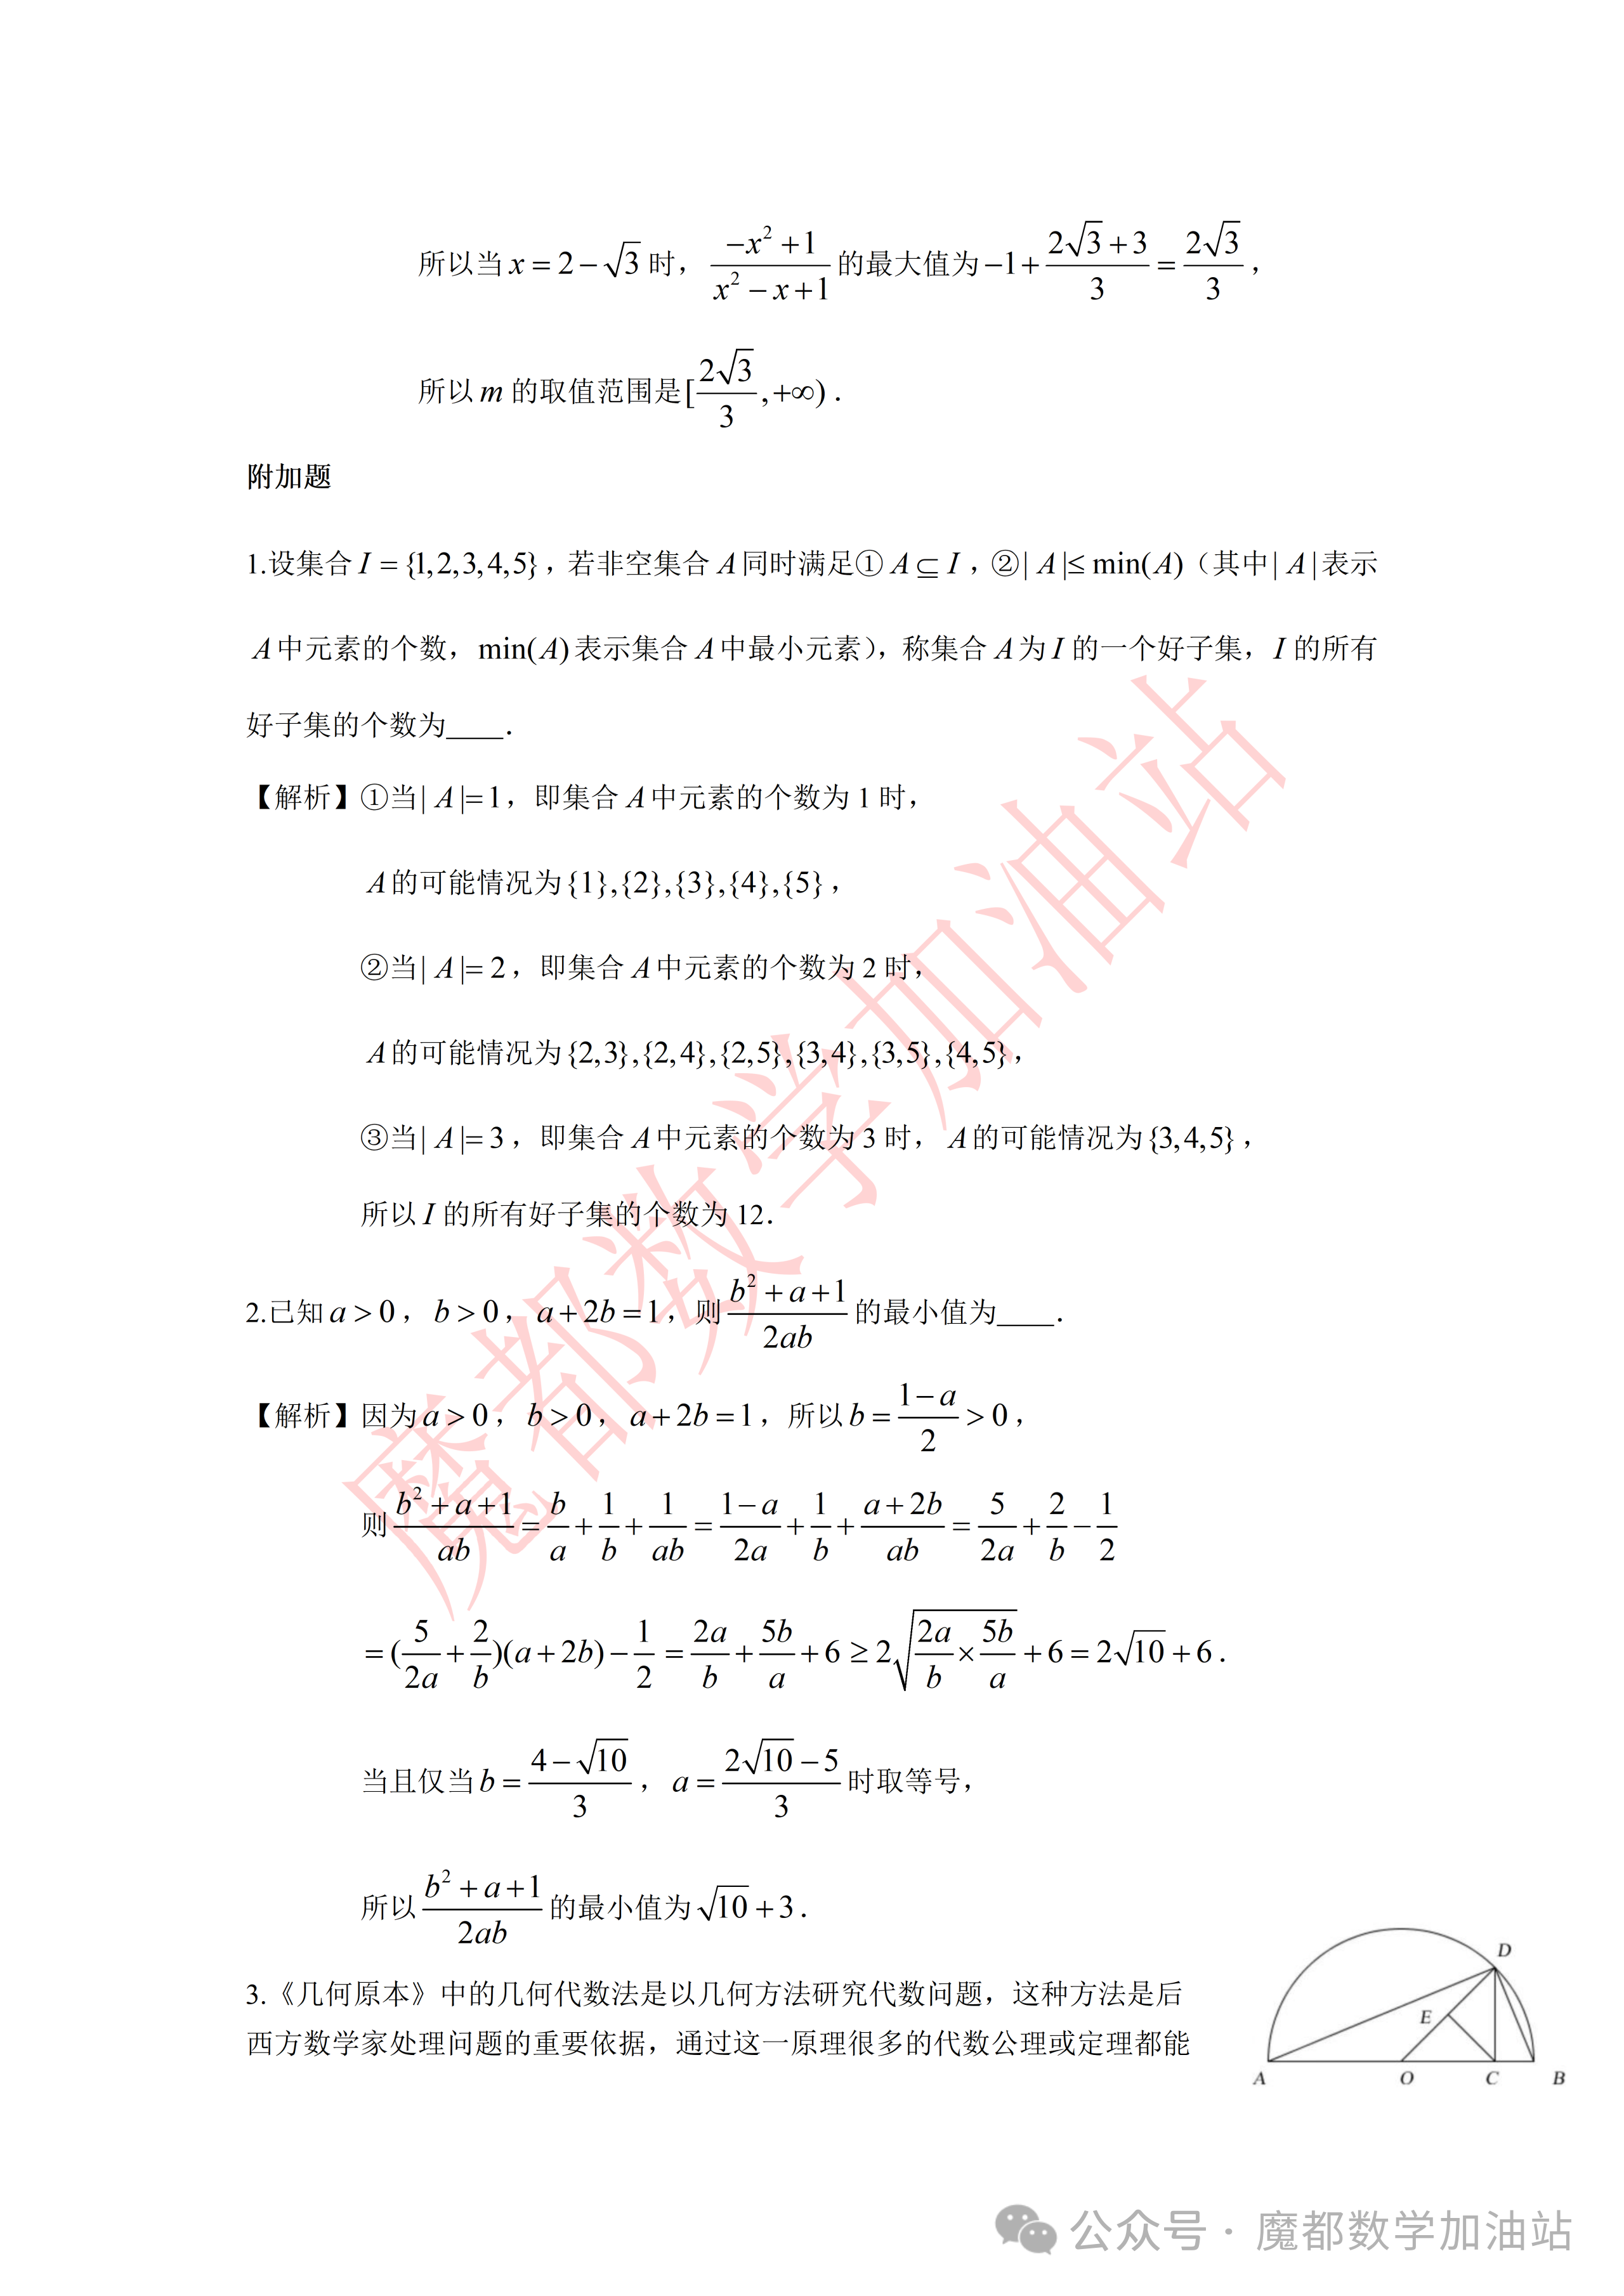
\includegraphics[width=.34\linewidth,trim=1960bp 310bp 90bp 3015bp,clip]{../原图/高一47_七宝中学_抱孩子练习9.26/08.png}
\end{center}

① $\dfrac{a+b}{2}\geqslant\sqrt{ab}$（$a>0$，$b>0$）；
② $a^2+b^2\geqslant2ab$（$a>0$，$b>0$）；
③ $\sqrt{ab}\geqslant\dfrac{2}{\dfrac1a+\dfrac1b}$（$a>0$，$b>0$）；
④ $\sqrt{\dfrac{a^2+b^2}{2}}\geqslant\dfrac{a+b}{2}$（$a>0$，$b>0$）.

\ifanswer
\solbegin
\step{因为 $AC+CB=a+b$，所以 $OD=\dfrac{AB}{2}=\dfrac{AC+CB}{2}=\dfrac{a+b}{2}$；}
\step{由射影定理得 $CD=\sqrt{AC\times CB}=\sqrt{ab}$，又因为 $OD\geqslant CD$，}
\step{所以 $\dfrac{a+b}{2}\geqslant\sqrt{ab}$，故①正确；}
\step{由射影定理得 $CD^2=DE\times OD$，所以 $DE=\dfrac{CD^2}{OD}=\dfrac{ab}{\dfrac{a+b}{2}}=\dfrac{2}{\dfrac1a+\dfrac1b}$，}
\step{又因为 $CD\geqslant DE$，所以 $\sqrt{ab}\geqslant\dfrac{2}{\dfrac1a+\dfrac1b}$，故③正确；}
\step{故该图形可以完成的所有无字证明为①③.}
\solend

\fi

% 注：原卷此处印作等式 $|x^2+a|+|x-a|=|x^2+x|$（在 $x>0$ 时与三角不等式下界等价），本稿曾改写成
% 不等式，现按原卷照录（原卷如此，照录未改）。
\item 若对任意 $x\in[2,3]$，均有 $|x^2+a|+|x-a|=|x^2+x|$，则实数 $a$ 的取值范围为 \blankline[4.4em].

\ifanswer
\solbegin
\step{因为 $|a|+|b|=|a+b|$ 当且仅当 $ab\geqslant0$ 时取等号，}
\step{所以 $(x^2+a)(x-a)\geqslant0$，即 $(a+x^2)(a-x)\leqslant0$，所以 $-x^2\leqslant a\leqslant x$ 恒成立，}
\step{因为 $x\in[2,3]$，所以 $-4\leqslant a\leqslant2$，所以实数 $a$ 的取值范围为 $[-4,2]$.}
\solend

\fi

\end{enumerate}

\end{document}
"
% 紧凑版：xelatex "\def\iscompact{1}% 高一47_七宝中学_抱孩子练习9.26.tex
%   —— 高一上数学“2026-2027 年七宝中学高一上抱孩子练习 9.26”（试卷版/答案版）
% 试卷版：xelatex 高一47_七宝中学_抱孩子练习9.26.tex
% 答案版：xelatex "\def\isanswer{1}% 高一47_七宝中学_抱孩子练习9.26.tex
%   —— 高一上数学“2026-2027 年七宝中学高一上抱孩子练习 9.26”（试卷版/答案版）
% 试卷版：xelatex 高一47_七宝中学_抱孩子练习9.26.tex
% 答案版：xelatex "\def\isanswer{1}\input{高一47_七宝中学_抱孩子练习9.26.tex}"
% 紧凑版：xelatex "\def\iscompact{1}\input{高一47_七宝中学_抱孩子练习9.26.tex}"
%
% 原始材料是微信公众号图文（公众号“魔都数学加油站”连载“27学年高一47”，署名“破晓”，
% 2026-10-02 17:56 发布，原文标题“27学年高一47——2026-2027年上海市七宝中学高一上抱孩子练习9.26”，
% 原文链接 https://mp.weixin.qq.com/s/mhkyDwjn7QFP_Z_NOcPkQA），正文为 9 张 PNG 页。
% 第 1—7、9 页分辨率为 4762×6735，第 8 页为 2560×3620；均按原图逐页核对。
% 原卷文字、选项、答案与解析均照录；粉色斜水印及灰色公众号页脚属水印/页脚，未录入。
%
% 卷首标题：原卷印作“2026-2027 年七宝中学高一上抱孩子练习 9.26”（公众号标题里的“上海市”
% 三字卷面标题行没有，本稿照卷面），年份区间按全稿惯例排 en dash，作业名保留原卷日期“9.26”。
% 原卷未印独立副标题；本稿按“知识模块”口径补出“集合与常用逻辑用语、不等式”。
%
% 与原卷的排版差异：
%   ① 原卷分“一、填空题”“二、选择题”“三、解答题”“附加题”四节；前三节题号为 3—16，
%      分别有 8 道填空、3 道选择、3 道解答；附加题另起 1—4 编号；
%   ② 原卷题下直接印答案/解析，本稿按全稿统一收进答案版；填空横线采用统一长度；
%   ③ 原卷未印副标题，本稿按“知识模块”口径补出（见卷首标题）；
%   ④ 全卷只有附加题第 3 题带图，直接从原卷第 8 页裁取。
%
% 原卷存疑（照录未改，见源码中该处上方注释）：
%   ① 第 9 题集合 C 的条件原文作“C={x|y=..., x 是整数}”，其中 y 未在集合描述中定义；
%      本稿照录原记号，未代换为 x。
%   ② 附加题第 3 题原文作“后西方数学家”，措辞存疑（疑漏“世”字）；本稿照录未改。
%
\documentclass[a4paper,11pt]{article}
\usepackage{common}

\begin{document}

\examtitlest[3]{2026--2027 年七宝中学高一上抱孩子练习 9.26}{集合与常用逻辑用语、不等式}

\bigsec{一、填空题}

\begin{enumerate}
\setcounter{enumi}{2}

\item 若不等式 $|x|<a$ 的一个充分条件为 $0<x<1$，则实数 $a$ 的取值范围是 \blankline[4.4em].

\ifanswer
\solbegin
\step{由 $|x|<a$ 得到 $-a<x<a$，}
\step{又不等式 $|x|<a$ 的一个充分条件为 $0<x<1$，所以 $a\geqslant1$.}
\solend

\fi

\item 已知命题“$\exists x\in\R$，使 $4x^2+(a-2)x+\dfrac14=0$”是假命题，则实数 $a$ 的取值范围是 \blankline[4.4em].

\ifanswer
\solbegin
% 注：原卷首句作“为真命题”（先按命题为真推出 $\Delta\geqslant0$，再由其为假得 $0<a<4$），原卷如此，照录未改。
\step{命题 $\exists x\in\R$，使 $4x^2+(a-2)x+\dfrac14=0$ 为真命题，}
\step{则 $\Delta=(a-2)^2-4\times4\times\dfrac14=a^2-4a\geqslant0$，解得 $a\leqslant0$ 或 $a\geqslant4$，}
\step{而命题“$\exists x\in\R$，使 $4x^2+(a-2)x+\dfrac14=0$”是假命题，则 $0<a<4$，}
\step{所以实数 $a$ 的取值范围是 $\{a\mid0<a<4\}$.}
\solend

\fi

\item 已知集合 $A=\{x\mid(a-1)x^2+3x-2=0\}$ 有且仅有两个子集，则实数 $a=$ \blankline[4.4em].

\ifanswer
\solbegin
\step{集合 $A=\{x\mid(a-1)x^2+3x-2=0\}$ 有且仅有两个不同的子集，}
\step{所以 $a-1=0$ 或 $\begin{cases}a-1\neq0\\\Delta=9+8(a-1)=0\end{cases}$，解得实数 $a=1$ 或 $a=-\dfrac18$.}
\solend

\fi

\item 已知函数 $y=x^2+bx+3$（其中 $b$ 是实数）中，$y$ 的取值范围是 $[0,+\infty)$，若关于 $x$ 的不等式 $x^2+bx+3<c$ 的解集为 $m-8<x<m$，则实数 $c$ 的值为 \blankline[4.4em].

\ifanswer
\solbegin
\step{因为 $y$ 的取值范围是 $[0,+\infty)$，所以 $\Delta=b^2-12=0$，解得 $b^2=12$，}
\step{因为不等式 $x^2+bx+3<c$ 的解集为 $m-8<x<m$，}
\step{令 $x^2+bx+3=c$，即 $x^2+bx+3-c=0$，方程的两根为 $x_1=m-8$，$x_2=m$，}
\step{所以 $|x_2-x_1|=\sqrt{(x_1+x_2)^2-4x_1x_2}=\sqrt{b^2-4(3-c)}=8$，即 $\sqrt{12-4(3-c)}=8$，}
\step{且判别式 $\Delta=b^2-4(3-c)=12-4(3-c)>0$，解得 $c=16$.}
\solend

\fi

\item 关于 $x$ 的不等式 $|x-1|+|x+1|\geqslant a$ 的解集为 $\R$，则实数 $a$ 的取值范围为 \blankline[4.4em].

\ifanswer
\solbegin
\step{因为 $|x-1|+|x+1|\geqslant|x-1-(x+1)|=2$，}
\step{若关于 $x$ 的不等式 $|x-1|+|x+1|\geqslant a$ 的解集为 $\R$，则实数 $a$ 的取值范围为 $a\leqslant2$.}
\solend

\fi

\item 已知 $m>0$，$xy>0$，当 $x+y=2$ 时，不等式 $\dfrac2x+\dfrac my\geqslant4$ 恒成立，则 $m$ 的取值范围是 \blankline[4.4em].

\ifanswer
\solbegin
\step{因为 $m>0$，$xy>0$，$x+y=2$，}
\step{所以 $\dfrac2x+\dfrac my=\dfrac12(x+y)\left(\dfrac2x+\dfrac my\right)
=\dfrac12\left(m+2+\dfrac{2y}{x}+\dfrac{mx}{y}\right)$}
\step{$\geqslant\dfrac12\left(m+2+2\sqrt{\dfrac{2y}{x}\cdot\dfrac{mx}{y}}\right)=\dfrac12\left(m+2+2\sqrt{2m}\right)$，}
\step{当且仅当 $\dfrac{2y}{x}=\dfrac{mx}{y}$，即 $y^2=\dfrac{mx^2}{2}$ 时取等号.}
\step{因为不等式 $\dfrac2x+\dfrac my\geqslant4$ 恒成立，所以 $\dfrac12(m+2+2\sqrt{2m})\geqslant4$，}
\step{整理得 $(\sqrt m+3\sqrt2)(\sqrt m-\sqrt2)\geqslant0$，解得 $\sqrt m\geqslant\sqrt2$，即 $m\geqslant2$，}
\step{所以 $m$ 的取值范围为 $[2,+\infty)$.}
\solend

\fi

\item 已知全集为 $\R$，集合 $D=\{x\mid x^2-ax+a^2-19=0\}$，
$B=\{y\mid y=-x^2+2x+2,\ y\text{ 是正整数}\}$，
% 注：本题集合 C 的条件原文作“C={x|y=..., x 是整数}”，其中 y 未在集合描述中定义；照录未改。
集合 $C=\left\{x\mathrel{\Big|}y=\sqrt{\dfrac{2-x}{x+1}},\ x\text{ 是整数}\right\}$，且集合 $D$ 满足 $D\cap B\neq\varnothing$，$\overline{D}\cup\overline{C}=\R$，则实数 $a$ 的值是 \blankline[4.4em].

\ifanswer
\solbegin
\step{集合 $B=\{y\mid y=-x^2+2x+2,\ y\text{ 是正整数}\}=\{1,2,3\}$，}
\step{集合 $C=\left\{x\mathrel{\Big|}y=\sqrt{\dfrac{2-x}{x+1}},\ x\text{ 是整数}\right\}=\{0,1,2\}$，}
\step{集合 $D=\{x\mid x^2-ax+a^2-19=0\}$ 且集合 $D$ 满足 $D\cap B\neq\varnothing$，$\overline{D}\cup\overline{C}=\R$，}
\step{所以 $3\in D$，解得 $a=5$ 或 $a=-2$，}
\step{经检验，$a=5$ 不符合 $\overline{D}\cup\overline{C}=\R$，舍去，$a=-2$ 满足题意，即 $a=-2$.}
\solend

\fi

% 注：本题解析中，$a=\pm2\sqrt2$ 时 $B$ 的二重根按 $-\dfrac a2$ 应为 $\mp\sqrt2$，原卷印作 $\mp2\sqrt2$、
% $-\dfrac{3\sqrt2}4$，$C(B)=3$ 的计算也随之按原卷保留（原卷如此，照录未改）。
\item 用 $C(A)$ 表示非空集合 $A$ 中的元素的个数，定义 $A*B=|C(A)-C(B)|$，已知集合 $A$ 有三个真子集，
$B=\{x\mid(ax^2+3x)(x^2+ax+2)=0,\ x\in\R\}$，若 $A*B=1$，设实数 $a$ 所有可能取值构成集合 $S$，则 $C(S)=$ \blankline[4.4em].

\ifanswer
\solbegin
\step{集合 $A$ 有三个真子集，则集合 $A$ 中有 $2$ 个元素，则 $C(A)=2$，}
\step{由 $A*B=1$，得 $C(B)=1$ 或 $3$，}
\step{即方程 $(ax^2+3x)\cdot(x^2+ax+2)=0$ 有一个根或 $3$ 个根；}
\step{若 $(ax^2+3x)\cdot(x^2+ax+2)=0$，则必有 $ax^2+3x=0$ 或 $x^2+ax+2=0$，}
\step{若 $ax^2+3x=0$，则 $x=0$ 或 $ax+3=0$，}
\step{当 $a=0$ 时，$B=\{0\}$，$C(B)=1$，符合题意；}
\step{当 $a\neq0$ 时，$ax^2+3x=0$ 对应的根为 $0$ 和 $-\dfrac3a$；}
\step{故①需 $x^2+ax+2=0$ 有两等根且根不为 $0$ 和 $-\dfrac3a$，}
\step{当 $\Delta=0$ 时，$a=\pm2\sqrt2$，}
\step{$a=2\sqrt2$，此时 $B=\left\{0,-2\sqrt2,-\dfrac{3\sqrt2}{4}\right\}$，$C(B)=3$，符合题意；}
\step{$a=-2\sqrt2$，此时 $B=\left\{0,2\sqrt2,\dfrac{3\sqrt2}{4}\right\}$，$C(B)=3$，符合题意；}
\step{②当 $-\dfrac3a$ 是 $x^2+ax+2=0$ 的根时，解得 $a=\pm3$；}
\step{$a=3$，此时 $B=\{0,-1,-2\}$，$C(B)=3$，符合题意；}
\step{$a=-3$，此时 $B=\{0,1,2\}$，$C(B)=3$，符合题意；}
\step{综上，$a$ 可取的值为 $0$、$\pm3$、$\pm2\sqrt2$，则 $C(S)=5$.}
\solend

\fi

\end{enumerate}

\bigsec{二、选择题}

\begin{enumerate}
\setcounter{enumi}{10}

\item 已知集合 $A=\left\{x\mathrel{\Big|}\dfrac1x<1\right\}$，$B=\{x\mid x^2-2x-3\leqslant0\}$，则 $A\cap B=$\mbox{（\quad）}

\keepwithprev
A. $\{x\mid1<x\leqslant3\}$\qquad B. $\{x\mid1\leqslant x\leqslant3\text{ 或 }-1\leqslant x<0\}$

C. $\{x\mid-1\leqslant x<0\}$\qquad D. $\{x\mid1<x\leqslant3\text{ 或 }-1\leqslant x<0\}$

\ans{$D$}

% 注：原卷本题只有题干＋选项（答案印在括号内），没有解析；此处照录原卷的"无解析"状态，不排解析。
\item 使 $x(y-2)=0$ 成立的一个充分条件是\mbox{（\quad）}

\keepwithprev
A. $x^2+(y-2)^2=0$\qquad B. $(x-2)^2+y^2=0$

C. $x^2+y^2=1$\qquad D. $x+y-2=0$

\ans{$A$}

\ifanswer
\solbegin
\step{对于 $A$：若 $x^2+(y-2)^2=0$，则 $x=0$ 且 $y=2$，此时 $x(y-2)=0$ 成立，}
\step{即充分性成立.}
\step{若 $x(y-2)=0$，则 $x=0$ 或 $y=2$，当 $x=0$，$y=3$ 时，$x^2+(y-2)^2=0$ 不成立，}
\step{即必要性不成立，}
\step{故 $x^2+(y-2)^2=0$ 是 $x(y-2)=0$ 成立的充分不必要条件；}
\step{对于 $B$：$(x-2)^2+y^2=0$，则 $x=2$ 且 $y=0$，此时 $x(y-2)=0$ 不成立，}
\step{即充分性不成立；}
\step{对于 $C$：$x^2+y^2=1$，此时 $x(y-2)=0$ 不一定成立，即充分性不成立；}
\step{对于 $D$：$x+y-2=0$，此时 $x(y-2)=0$ 不一定成立，即充分性不成立.}
\step{故选 $A$.}
\solend

\fi

\item 已知 $a$、$b$、$c\in\R$，若关于 $x$ 的不等式 $0\leqslant x+\dfrac ax+b\leqslant\dfrac cx-1$ 的解集为 $[x_1,x_2]\cup\{x_3\}$（$x_3>x_2>x_1>0$），则\mbox{（\quad）}

\keepwithprev
A. 不存在有序数组 $(a,b,c)$，使得 $x_2-x_1=1$

B. 存在唯一有序数组 $(a,b,c)$，使得 $x_2-x_1=1$

C. 有且只有两组有序数组 $(a,b,c)$，使得 $x_2-x_1=1$

D. 存在无穷多组有序数组 $(a,b,c)$，使得 $x_2-x_1=1$

\ans{$D$}

\ifanswer
\solbegin
\step{因为不等式 $0\leqslant x+\dfrac ax+b\leqslant\dfrac cx-1$ 的解集为 $[x_1,x_2]\cup\{x_3\}$（$x_3>x_2>x_1>0$），}
\step{所以 $0\leqslant x^2+bx+a\leqslant c-x$ 在 $[x_1,x_2]\cup\{x_3\}$ 上成立，}
\step{假设 $x_1=m$，$x_2=m+1$，$x_3=n$，}
\step{则 $c-n=0=n^2+bn+a$，由 $x_3$ 为一个独立的数得出，}
\step{所以 $n=c$，且 $m+1$ 与 $n$ 为方程 $x^2+bx+a=0$ 的两个根，}
\step{因为 $x_3>x_2>x_1>0$，所以 $-b=m+n+1=m+c+1$，$a=mn+n=mc+c$，}
\step{所以 $b=-m-c-1$，}
\step{且点 $(x_1,x_1^2+bx_1+a)$ 为 $y=x^2+bx+a$ 与 $y=c-x$ 的左交点，}
\step{所以 $m^2+bm+a=c-m$ 且 $b=-m-c-1$，$a=mc+c$，}
% 注：原卷此行的末句作“所以 $c-m=c-m$ 恒成立”（未写成 $x_2-x_1=1$），原卷如此，照录未改。
\step{故 $m^2+bm+a=m^2-m^2-mc-m+mc+c=c-m$，所以 $c-m=c-m$ 恒成立，}
\step{所以不论 $a$、$b$、$c$ 取何值，$x_2-x_1=1$ 恒成立，}
\step{即存在无穷多组有序数组 $(a,b,c)$，使得 $x_2-x_1=1$，}
\step{故选项 $A$、$B$、$C$ 错误，选项 $D$ 正确. 故选 $D$.}
\solend

\fi

\end{enumerate}

\bigsec{三、解答题}

\begin{enumerate}
\setcounter{enumi}{13}

\item 设正实数 $x$、$y$，满足 $2x+y=1$，求：

\begin{enumerate}[label=(\arabic*)]
\item $\sqrt{2x}+\sqrt y$ 的最大值；
\item $\dfrac2x+\dfrac1y$ 的最小值.
\end{enumerate}

\ifanswer
\solbegin
\stepm{(1)}{对于 $(\sqrt{2x}+\sqrt y)^2=2x+y+2\sqrt{2xy}\leqslant1+1=2$，}
\step{当且仅当 $\sqrt{2x}=\sqrt y$ 时取等号，故 $\sqrt{2x}+\sqrt y$ 的最大值为 $\sqrt2$；}
\stepm{(2)}{$\dfrac2x+\dfrac1y=\left(\dfrac2x+\dfrac1y\right)(2x+y)=5+\dfrac{2y}{x}+\dfrac{2x}{y}\geqslant5+4=9$，}
\step{当且仅当 $\dfrac{2y}{x}=\dfrac{2x}{y}$，即 $x=y=\dfrac13$ 时取等号，故 $\dfrac2x+\dfrac1y$ 的最小值为 $9$.}
\solend

\fi

\ansspace[6]

\item 设 $x_1$、$x_2$ 为关于 $x$ 的方程 $x^2-2(m+2)x+m^2-1=0$ 的两实数根.

\begin{enumerate}[label=(\arabic*)]
\item 若 $x_1$、$x_2$ 满足 $x_1^2+x_2^2=18$，试求 $m$ 的值；
\item 若 $x_1$、$x_2$ 均大于 $0$，求 $m$ 的取值范围.
\end{enumerate}

\ifanswer
\solbegin
\stepm{(1)}{由 $\Delta=4(m+2)^2-4(m^2-1)\geqslant0$，解得 $m\geqslant-\dfrac54$，}
\step{由韦达定理得 $x_1+x_2=2(m+2)$，$x_1x_2=m^2-1$，}
\step{又 $x_1^2+x_2^2=(x_1+x_2)^2-2x_1x_2=4(m+2)^2-2(m^2-1)=18$，}
\step{即 $m^2+8m=0$，解得 $m=0$ 或 $m=-8$（舍），故 $m$ 的值为 $0$；}
% 注：原卷此处作“由（2）得”（对照上一小问，所指应为（1）），原卷如此，照录未改。
\stepm{(2)}{由（2）得 $m\geqslant-\dfrac54$，}
\step{又 $x_1$、$x_2$ 均大于 $0$，则 $\begin{cases}2(m+2)>0\\m^2-1>0\end{cases}$，解得 $\begin{cases}m>-2\\m>1\text{或}m<-1\end{cases}$，}
\step{综上，实数 $m$ 的取值范围为 $\left[-\dfrac54,-1\right)\cup(1,+\infty)$.}
\solend

\fi

\ansspace[6]

\item 已知函数 $f(x)=(m+1)x^2-mx+m-1$（$m\in\R$）.

\begin{enumerate}[label=(\arabic*)]
\item 若不等式 $f(x)<0$ 的解集是空集，求 $m$ 的取值范围；
\item 当 $m>-2$ 时，解不等式 $f(x)\geqslant m$；
\item 若不等式 $f(x)\geqslant0$ 的解集为 $D$，若 $[-1,1]\subseteq D$，求 $m$ 的取值范围.
\end{enumerate}

\ifanswer
\solbegin
\stepm{(1)}{①当 $m+1=0$，即 $m=-1$ 时，$f(x)=x-2$，不合题意；}
\step{②当 $m+1\neq0$，即 $m\neq-1$ 时，$\begin{cases}m+1>0\\\Delta=m^2-4(m+1)(m-1)\leqslant0\end{cases}$，解得 $m\geqslant\dfrac{2\sqrt3}{3}$，}
\step{所以 $m$ 的取值范围是 $\left[\dfrac{2\sqrt3}{3},+\infty\right)$；}
\stepm{(2)}{因为 $f(x)\geqslant m$，所以 $(m+1)x^2-mx-1\geqslant0$，即 $[(m+1)x+1](x-1)\geqslant0$，}
\step{①当 $m+1=0$ 即 $m=-1$ 时，不等式的解集为 $[1,+\infty)$；}
\step{②当 $m+1>0$ 即 $m>-1$ 时，$\left(x+\dfrac1{m+1}\right)(x-1)\geqslant0$，}
\step{因为 $-\dfrac1{m+1}<0$，所以不等式的解集为 $\left(-\infty,-\dfrac1{m+1}\right]\cup[1,+\infty)$；}
\step{③当 $m+1<0$ 即 $-2<m<-1$ 时，$\left(x+\dfrac1{m+1}\right)(x-1)\leqslant0$，}
\step{因为 $-2<m<-1$，所以 $-1<m+1<0$，所以 $-\dfrac1{m+1}>1$，}
\step{所以不等式的解集为 $\left[1,-\dfrac1{m+1}\right]$；}
\stepm{(3)}{不等式 $f(x)\geqslant0$ 的解集为 $D$，若 $[-1,1]\subseteq D$，}
\step{即对任意的 $x\in[-1,1]$，不等式 $(m+1)x^2-mx+m-1\geqslant0$ 恒成立，}
\step{即 $m(x^2-x+1)\geqslant-x^2+1$ 恒成立，}
\step{因为 $x^2-x+1>0$ 恒成立，所以 $m\geqslant\dfrac{-x^2+1}{x^2-x+1}=-1+\dfrac{2-x}{x^2-x+1}$ 恒成立，}
\step{设 $t=2-x$，则 $t\in[1,3]$，$x=2-t$，}
\step{则 $\dfrac{2-x}{x^2-x+1}=\dfrac{t}{(2-t)^2-(2-t)+1}=\dfrac{t}{t^2-3t+3}=\dfrac1{t+\dfrac3t-3}$，}
\step{因为 $t+\dfrac3t\geqslant2\sqrt3$，当且仅当 $t=\sqrt3$ 时取等号，}
\step{所以 $\dfrac{2-x}{x^2-x+1}\leqslant\dfrac1{2\sqrt3-3}=\dfrac{2\sqrt3+3}{3}$，当且仅当 $x=2-\sqrt3$ 时取等号，}
\step{所以当 $x=2-\sqrt3$ 时，$\dfrac{-x^2+1}{x^2-x+1}$ 的最大值为 $-1+\dfrac{2\sqrt3+3}{3}=\dfrac{2\sqrt3}{3}$，}
\step{所以 $m$ 的取值范围是 $\left[\dfrac{2\sqrt3}{3},+\infty\right)$.}
\solend

\fi

\ansspace[8]

\end{enumerate}

\bigsec{附加题}

\begin{enumerate}

\item 设集合 $I=\{1,2,3,4,5\}$，若非空集合 $A$ 同时满足① $A\subseteq I$，② $|A|\leqslant\min(A)$（其中 $|A|$ 表示集合 $A$ 中元素的个数，$\min(A)$ 表示集合 $A$ 中最小元素），称集合 $A$ 为 $I$ 的一个好子集，$I$ 所有好子集的个数为 \blankline[4.4em].

\ifanswer
\solbegin
\step{①当 $|A|=1$，即集合 $A$ 中元素的个数为 $1$ 时，}
\step{$A$ 的可能情况为 $\{1\}$、$\{2\}$、$\{3\}$、$\{4\}$、$\{5\}$，}
\step{②当 $|A|=2$，即集合 $A$ 中元素的个数为 $2$ 时，}
\step{$A$ 的可能情况为 $\{2,3\}$、$\{2,4\}$、$\{2,5\}$、$\{3,4\}$、$\{3,5\}$、$\{4,5\}$，}
\step{③当 $|A|=3$，即集合 $A$ 中元素的个数为 $3$ 时，$A$ 的可能情况为 $\{3,4,5\}$，}
\step{所以 $I$ 的所有好子集的个数为 $12$.}
\solend

\fi

\item 已知 $a>0$，$b>0$，$a+2b=1$，则 $\dfrac{b^2+a+1}{2ab}$ 的最小值为 \blankline[4.4em].

\ifanswer
\solbegin
\step{因为 $a>0$，$b>0$，$a+2b=1$，所以 $b=\dfrac{1-a}{2}>0$，}
\step{则 $\dfrac{b^2+a+1}{ab}=\dfrac ba+\dfrac1b+\dfrac1{ab}=\dfrac{1-a}{2a}+\dfrac1b+\dfrac{a+2b}{ab}=\dfrac5{2a}+\dfrac2b-\dfrac12$}
\step{$=\left(\dfrac5{2a}+\dfrac2b\right)(a+2b)-\dfrac12=\dfrac{2a}{b}+\dfrac{5b}{a}+6\geqslant2\sqrt{\dfrac{2a}{b}\times\dfrac{5b}{a}}+6=2\sqrt{10}+6$.}
\step{当且仅当 $b=\dfrac{4-\sqrt{10}}{3}$，$a=\dfrac{2\sqrt{10}-5}{3}$ 时取等号，}
\step{所以 $\dfrac{b^2+a+1}{2ab}$ 的最小值为 $\sqrt{10}+3$.}
\solend

\fi

% 注：本题原文作“后西方数学家”，措辞存疑（疑漏“世”字）；照录未改，见文件头“原卷存疑”②。
% 又原文作"很多的代数公理或定理都能够通过图形实现证明"（"公理"疑为"公式"笔误）、
% "连结 OD,AD,BD"，均原卷如此，照录未改。
\item 《几何原本》中的几何代数法是以几何方法研究代数问题，这种方法是后西方数学家处理问题的重要依据，通过这一原理很多的代数公理或定理都能够通过图形实现证明，也称之为无字证明，现有图形如图所示，$C$ 为线段 $AB$ 上的点，且 $AC=a$，$BC=b$，$O$ 为 $AB$ 的中点，以 $AB$ 为直径作半圆，过点 $C$ 作 $AB$ 的垂线交半圆于 $D$，连结 $OD,AD,BD$，过点 $C$ 作 $OD$ 的垂线，垂足为 $E$，若不添加辅助线，则该图形可以完成的所有无字证明为 \blankline[4.4em]（填写序号）.

\begin{center}
% 插图直接裁自原卷第 8 页，未重绘；用 trim/clip 保留原图与标注。
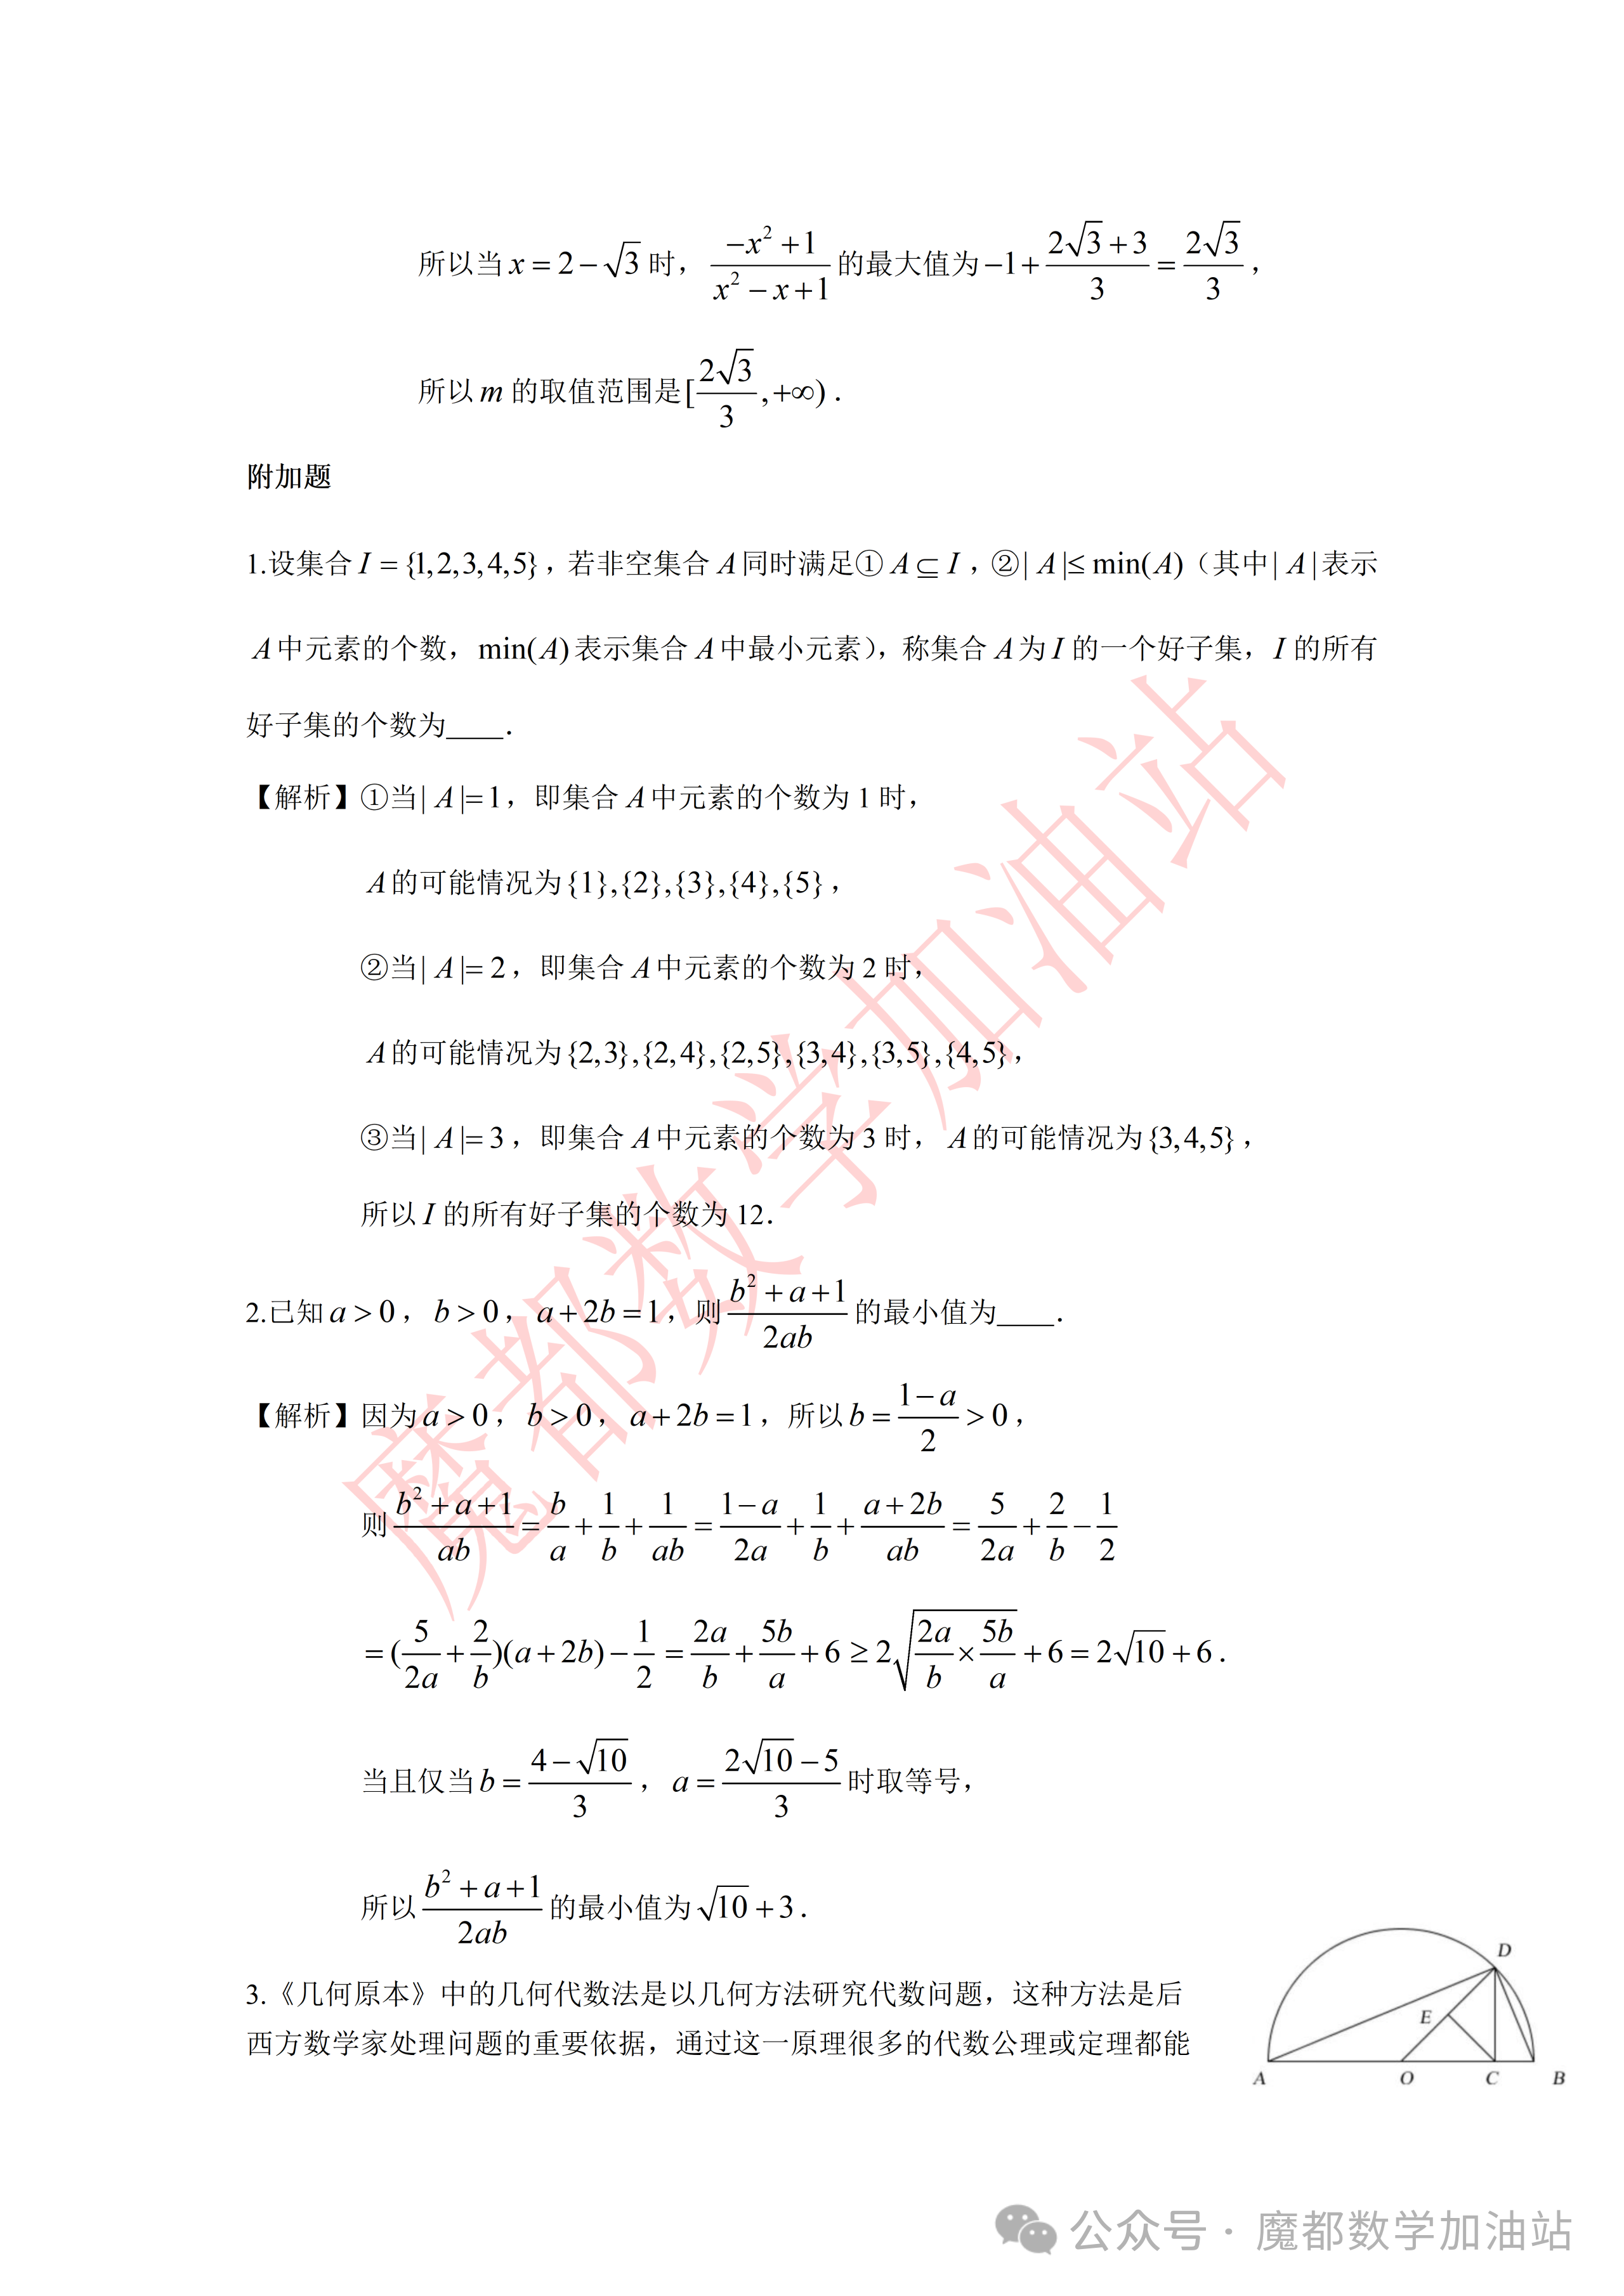
\includegraphics[width=.34\linewidth,trim=1960bp 310bp 90bp 3015bp,clip]{../原图/高一47_七宝中学_抱孩子练习9.26/08.png}
\end{center}

① $\dfrac{a+b}{2}\geqslant\sqrt{ab}$（$a>0$，$b>0$）；
② $a^2+b^2\geqslant2ab$（$a>0$，$b>0$）；
③ $\sqrt{ab}\geqslant\dfrac{2}{\dfrac1a+\dfrac1b}$（$a>0$，$b>0$）；
④ $\sqrt{\dfrac{a^2+b^2}{2}}\geqslant\dfrac{a+b}{2}$（$a>0$，$b>0$）.

\ifanswer
\solbegin
\step{因为 $AC+CB=a+b$，所以 $OD=\dfrac{AB}{2}=\dfrac{AC+CB}{2}=\dfrac{a+b}{2}$；}
\step{由射影定理得 $CD=\sqrt{AC\times CB}=\sqrt{ab}$，又因为 $OD\geqslant CD$，}
\step{所以 $\dfrac{a+b}{2}\geqslant\sqrt{ab}$，故①正确；}
\step{由射影定理得 $CD^2=DE\times OD$，所以 $DE=\dfrac{CD^2}{OD}=\dfrac{ab}{\dfrac{a+b}{2}}=\dfrac{2}{\dfrac1a+\dfrac1b}$，}
\step{又因为 $CD\geqslant DE$，所以 $\sqrt{ab}\geqslant\dfrac{2}{\dfrac1a+\dfrac1b}$，故③正确；}
\step{故该图形可以完成的所有无字证明为①③.}
\solend

\fi

% 注：原卷此处印作等式 $|x^2+a|+|x-a|=|x^2+x|$（在 $x>0$ 时与三角不等式下界等价），本稿曾改写成
% 不等式，现按原卷照录（原卷如此，照录未改）。
\item 若对任意 $x\in[2,3]$，均有 $|x^2+a|+|x-a|=|x^2+x|$，则实数 $a$ 的取值范围为 \blankline[4.4em].

\ifanswer
\solbegin
\step{因为 $|a|+|b|=|a+b|$ 当且仅当 $ab\geqslant0$ 时取等号，}
\step{所以 $(x^2+a)(x-a)\geqslant0$，即 $(a+x^2)(a-x)\leqslant0$，所以 $-x^2\leqslant a\leqslant x$ 恒成立，}
\step{因为 $x\in[2,3]$，所以 $-4\leqslant a\leqslant2$，所以实数 $a$ 的取值范围为 $[-4,2]$.}
\solend

\fi

\end{enumerate}

\end{document}
"
% 紧凑版：xelatex "\def\iscompact{1}% 高一47_七宝中学_抱孩子练习9.26.tex
%   —— 高一上数学“2026-2027 年七宝中学高一上抱孩子练习 9.26”（试卷版/答案版）
% 试卷版：xelatex 高一47_七宝中学_抱孩子练习9.26.tex
% 答案版：xelatex "\def\isanswer{1}\input{高一47_七宝中学_抱孩子练习9.26.tex}"
% 紧凑版：xelatex "\def\iscompact{1}\input{高一47_七宝中学_抱孩子练习9.26.tex}"
%
% 原始材料是微信公众号图文（公众号“魔都数学加油站”连载“27学年高一47”，署名“破晓”，
% 2026-10-02 17:56 发布，原文标题“27学年高一47——2026-2027年上海市七宝中学高一上抱孩子练习9.26”，
% 原文链接 https://mp.weixin.qq.com/s/mhkyDwjn7QFP_Z_NOcPkQA），正文为 9 张 PNG 页。
% 第 1—7、9 页分辨率为 4762×6735，第 8 页为 2560×3620；均按原图逐页核对。
% 原卷文字、选项、答案与解析均照录；粉色斜水印及灰色公众号页脚属水印/页脚，未录入。
%
% 卷首标题：原卷印作“2026-2027 年七宝中学高一上抱孩子练习 9.26”（公众号标题里的“上海市”
% 三字卷面标题行没有，本稿照卷面），年份区间按全稿惯例排 en dash，作业名保留原卷日期“9.26”。
% 原卷未印独立副标题；本稿按“知识模块”口径补出“集合与常用逻辑用语、不等式”。
%
% 与原卷的排版差异：
%   ① 原卷分“一、填空题”“二、选择题”“三、解答题”“附加题”四节；前三节题号为 3—16，
%      分别有 8 道填空、3 道选择、3 道解答；附加题另起 1—4 编号；
%   ② 原卷题下直接印答案/解析，本稿按全稿统一收进答案版；填空横线采用统一长度；
%   ③ 原卷未印副标题，本稿按“知识模块”口径补出（见卷首标题）；
%   ④ 全卷只有附加题第 3 题带图，直接从原卷第 8 页裁取。
%
% 原卷存疑（照录未改，见源码中该处上方注释）：
%   ① 第 9 题集合 C 的条件原文作“C={x|y=..., x 是整数}”，其中 y 未在集合描述中定义；
%      本稿照录原记号，未代换为 x。
%   ② 附加题第 3 题原文作“后西方数学家”，措辞存疑（疑漏“世”字）；本稿照录未改。
%
\documentclass[a4paper,11pt]{article}
\usepackage{common}

\begin{document}

\examtitlest[3]{2026--2027 年七宝中学高一上抱孩子练习 9.26}{集合与常用逻辑用语、不等式}

\bigsec{一、填空题}

\begin{enumerate}
\setcounter{enumi}{2}

\item 若不等式 $|x|<a$ 的一个充分条件为 $0<x<1$，则实数 $a$ 的取值范围是 \blankline[4.4em].

\ifanswer
\solbegin
\step{由 $|x|<a$ 得到 $-a<x<a$，}
\step{又不等式 $|x|<a$ 的一个充分条件为 $0<x<1$，所以 $a\geqslant1$.}
\solend

\fi

\item 已知命题“$\exists x\in\R$，使 $4x^2+(a-2)x+\dfrac14=0$”是假命题，则实数 $a$ 的取值范围是 \blankline[4.4em].

\ifanswer
\solbegin
% 注：原卷首句作“为真命题”（先按命题为真推出 $\Delta\geqslant0$，再由其为假得 $0<a<4$），原卷如此，照录未改。
\step{命题 $\exists x\in\R$，使 $4x^2+(a-2)x+\dfrac14=0$ 为真命题，}
\step{则 $\Delta=(a-2)^2-4\times4\times\dfrac14=a^2-4a\geqslant0$，解得 $a\leqslant0$ 或 $a\geqslant4$，}
\step{而命题“$\exists x\in\R$，使 $4x^2+(a-2)x+\dfrac14=0$”是假命题，则 $0<a<4$，}
\step{所以实数 $a$ 的取值范围是 $\{a\mid0<a<4\}$.}
\solend

\fi

\item 已知集合 $A=\{x\mid(a-1)x^2+3x-2=0\}$ 有且仅有两个子集，则实数 $a=$ \blankline[4.4em].

\ifanswer
\solbegin
\step{集合 $A=\{x\mid(a-1)x^2+3x-2=0\}$ 有且仅有两个不同的子集，}
\step{所以 $a-1=0$ 或 $\begin{cases}a-1\neq0\\\Delta=9+8(a-1)=0\end{cases}$，解得实数 $a=1$ 或 $a=-\dfrac18$.}
\solend

\fi

\item 已知函数 $y=x^2+bx+3$（其中 $b$ 是实数）中，$y$ 的取值范围是 $[0,+\infty)$，若关于 $x$ 的不等式 $x^2+bx+3<c$ 的解集为 $m-8<x<m$，则实数 $c$ 的值为 \blankline[4.4em].

\ifanswer
\solbegin
\step{因为 $y$ 的取值范围是 $[0,+\infty)$，所以 $\Delta=b^2-12=0$，解得 $b^2=12$，}
\step{因为不等式 $x^2+bx+3<c$ 的解集为 $m-8<x<m$，}
\step{令 $x^2+bx+3=c$，即 $x^2+bx+3-c=0$，方程的两根为 $x_1=m-8$，$x_2=m$，}
\step{所以 $|x_2-x_1|=\sqrt{(x_1+x_2)^2-4x_1x_2}=\sqrt{b^2-4(3-c)}=8$，即 $\sqrt{12-4(3-c)}=8$，}
\step{且判别式 $\Delta=b^2-4(3-c)=12-4(3-c)>0$，解得 $c=16$.}
\solend

\fi

\item 关于 $x$ 的不等式 $|x-1|+|x+1|\geqslant a$ 的解集为 $\R$，则实数 $a$ 的取值范围为 \blankline[4.4em].

\ifanswer
\solbegin
\step{因为 $|x-1|+|x+1|\geqslant|x-1-(x+1)|=2$，}
\step{若关于 $x$ 的不等式 $|x-1|+|x+1|\geqslant a$ 的解集为 $\R$，则实数 $a$ 的取值范围为 $a\leqslant2$.}
\solend

\fi

\item 已知 $m>0$，$xy>0$，当 $x+y=2$ 时，不等式 $\dfrac2x+\dfrac my\geqslant4$ 恒成立，则 $m$ 的取值范围是 \blankline[4.4em].

\ifanswer
\solbegin
\step{因为 $m>0$，$xy>0$，$x+y=2$，}
\step{所以 $\dfrac2x+\dfrac my=\dfrac12(x+y)\left(\dfrac2x+\dfrac my\right)
=\dfrac12\left(m+2+\dfrac{2y}{x}+\dfrac{mx}{y}\right)$}
\step{$\geqslant\dfrac12\left(m+2+2\sqrt{\dfrac{2y}{x}\cdot\dfrac{mx}{y}}\right)=\dfrac12\left(m+2+2\sqrt{2m}\right)$，}
\step{当且仅当 $\dfrac{2y}{x}=\dfrac{mx}{y}$，即 $y^2=\dfrac{mx^2}{2}$ 时取等号.}
\step{因为不等式 $\dfrac2x+\dfrac my\geqslant4$ 恒成立，所以 $\dfrac12(m+2+2\sqrt{2m})\geqslant4$，}
\step{整理得 $(\sqrt m+3\sqrt2)(\sqrt m-\sqrt2)\geqslant0$，解得 $\sqrt m\geqslant\sqrt2$，即 $m\geqslant2$，}
\step{所以 $m$ 的取值范围为 $[2,+\infty)$.}
\solend

\fi

\item 已知全集为 $\R$，集合 $D=\{x\mid x^2-ax+a^2-19=0\}$，
$B=\{y\mid y=-x^2+2x+2,\ y\text{ 是正整数}\}$，
% 注：本题集合 C 的条件原文作“C={x|y=..., x 是整数}”，其中 y 未在集合描述中定义；照录未改。
集合 $C=\left\{x\mathrel{\Big|}y=\sqrt{\dfrac{2-x}{x+1}},\ x\text{ 是整数}\right\}$，且集合 $D$ 满足 $D\cap B\neq\varnothing$，$\overline{D}\cup\overline{C}=\R$，则实数 $a$ 的值是 \blankline[4.4em].

\ifanswer
\solbegin
\step{集合 $B=\{y\mid y=-x^2+2x+2,\ y\text{ 是正整数}\}=\{1,2,3\}$，}
\step{集合 $C=\left\{x\mathrel{\Big|}y=\sqrt{\dfrac{2-x}{x+1}},\ x\text{ 是整数}\right\}=\{0,1,2\}$，}
\step{集合 $D=\{x\mid x^2-ax+a^2-19=0\}$ 且集合 $D$ 满足 $D\cap B\neq\varnothing$，$\overline{D}\cup\overline{C}=\R$，}
\step{所以 $3\in D$，解得 $a=5$ 或 $a=-2$，}
\step{经检验，$a=5$ 不符合 $\overline{D}\cup\overline{C}=\R$，舍去，$a=-2$ 满足题意，即 $a=-2$.}
\solend

\fi

% 注：本题解析中，$a=\pm2\sqrt2$ 时 $B$ 的二重根按 $-\dfrac a2$ 应为 $\mp\sqrt2$，原卷印作 $\mp2\sqrt2$、
% $-\dfrac{3\sqrt2}4$，$C(B)=3$ 的计算也随之按原卷保留（原卷如此，照录未改）。
\item 用 $C(A)$ 表示非空集合 $A$ 中的元素的个数，定义 $A*B=|C(A)-C(B)|$，已知集合 $A$ 有三个真子集，
$B=\{x\mid(ax^2+3x)(x^2+ax+2)=0,\ x\in\R\}$，若 $A*B=1$，设实数 $a$ 所有可能取值构成集合 $S$，则 $C(S)=$ \blankline[4.4em].

\ifanswer
\solbegin
\step{集合 $A$ 有三个真子集，则集合 $A$ 中有 $2$ 个元素，则 $C(A)=2$，}
\step{由 $A*B=1$，得 $C(B)=1$ 或 $3$，}
\step{即方程 $(ax^2+3x)\cdot(x^2+ax+2)=0$ 有一个根或 $3$ 个根；}
\step{若 $(ax^2+3x)\cdot(x^2+ax+2)=0$，则必有 $ax^2+3x=0$ 或 $x^2+ax+2=0$，}
\step{若 $ax^2+3x=0$，则 $x=0$ 或 $ax+3=0$，}
\step{当 $a=0$ 时，$B=\{0\}$，$C(B)=1$，符合题意；}
\step{当 $a\neq0$ 时，$ax^2+3x=0$ 对应的根为 $0$ 和 $-\dfrac3a$；}
\step{故①需 $x^2+ax+2=0$ 有两等根且根不为 $0$ 和 $-\dfrac3a$，}
\step{当 $\Delta=0$ 时，$a=\pm2\sqrt2$，}
\step{$a=2\sqrt2$，此时 $B=\left\{0,-2\sqrt2,-\dfrac{3\sqrt2}{4}\right\}$，$C(B)=3$，符合题意；}
\step{$a=-2\sqrt2$，此时 $B=\left\{0,2\sqrt2,\dfrac{3\sqrt2}{4}\right\}$，$C(B)=3$，符合题意；}
\step{②当 $-\dfrac3a$ 是 $x^2+ax+2=0$ 的根时，解得 $a=\pm3$；}
\step{$a=3$，此时 $B=\{0,-1,-2\}$，$C(B)=3$，符合题意；}
\step{$a=-3$，此时 $B=\{0,1,2\}$，$C(B)=3$，符合题意；}
\step{综上，$a$ 可取的值为 $0$、$\pm3$、$\pm2\sqrt2$，则 $C(S)=5$.}
\solend

\fi

\end{enumerate}

\bigsec{二、选择题}

\begin{enumerate}
\setcounter{enumi}{10}

\item 已知集合 $A=\left\{x\mathrel{\Big|}\dfrac1x<1\right\}$，$B=\{x\mid x^2-2x-3\leqslant0\}$，则 $A\cap B=$\mbox{（\quad）}

\keepwithprev
A. $\{x\mid1<x\leqslant3\}$\qquad B. $\{x\mid1\leqslant x\leqslant3\text{ 或 }-1\leqslant x<0\}$

C. $\{x\mid-1\leqslant x<0\}$\qquad D. $\{x\mid1<x\leqslant3\text{ 或 }-1\leqslant x<0\}$

\ans{$D$}

% 注：原卷本题只有题干＋选项（答案印在括号内），没有解析；此处照录原卷的"无解析"状态，不排解析。
\item 使 $x(y-2)=0$ 成立的一个充分条件是\mbox{（\quad）}

\keepwithprev
A. $x^2+(y-2)^2=0$\qquad B. $(x-2)^2+y^2=0$

C. $x^2+y^2=1$\qquad D. $x+y-2=0$

\ans{$A$}

\ifanswer
\solbegin
\step{对于 $A$：若 $x^2+(y-2)^2=0$，则 $x=0$ 且 $y=2$，此时 $x(y-2)=0$ 成立，}
\step{即充分性成立.}
\step{若 $x(y-2)=0$，则 $x=0$ 或 $y=2$，当 $x=0$，$y=3$ 时，$x^2+(y-2)^2=0$ 不成立，}
\step{即必要性不成立，}
\step{故 $x^2+(y-2)^2=0$ 是 $x(y-2)=0$ 成立的充分不必要条件；}
\step{对于 $B$：$(x-2)^2+y^2=0$，则 $x=2$ 且 $y=0$，此时 $x(y-2)=0$ 不成立，}
\step{即充分性不成立；}
\step{对于 $C$：$x^2+y^2=1$，此时 $x(y-2)=0$ 不一定成立，即充分性不成立；}
\step{对于 $D$：$x+y-2=0$，此时 $x(y-2)=0$ 不一定成立，即充分性不成立.}
\step{故选 $A$.}
\solend

\fi

\item 已知 $a$、$b$、$c\in\R$，若关于 $x$ 的不等式 $0\leqslant x+\dfrac ax+b\leqslant\dfrac cx-1$ 的解集为 $[x_1,x_2]\cup\{x_3\}$（$x_3>x_2>x_1>0$），则\mbox{（\quad）}

\keepwithprev
A. 不存在有序数组 $(a,b,c)$，使得 $x_2-x_1=1$

B. 存在唯一有序数组 $(a,b,c)$，使得 $x_2-x_1=1$

C. 有且只有两组有序数组 $(a,b,c)$，使得 $x_2-x_1=1$

D. 存在无穷多组有序数组 $(a,b,c)$，使得 $x_2-x_1=1$

\ans{$D$}

\ifanswer
\solbegin
\step{因为不等式 $0\leqslant x+\dfrac ax+b\leqslant\dfrac cx-1$ 的解集为 $[x_1,x_2]\cup\{x_3\}$（$x_3>x_2>x_1>0$），}
\step{所以 $0\leqslant x^2+bx+a\leqslant c-x$ 在 $[x_1,x_2]\cup\{x_3\}$ 上成立，}
\step{假设 $x_1=m$，$x_2=m+1$，$x_3=n$，}
\step{则 $c-n=0=n^2+bn+a$，由 $x_3$ 为一个独立的数得出，}
\step{所以 $n=c$，且 $m+1$ 与 $n$ 为方程 $x^2+bx+a=0$ 的两个根，}
\step{因为 $x_3>x_2>x_1>0$，所以 $-b=m+n+1=m+c+1$，$a=mn+n=mc+c$，}
\step{所以 $b=-m-c-1$，}
\step{且点 $(x_1,x_1^2+bx_1+a)$ 为 $y=x^2+bx+a$ 与 $y=c-x$ 的左交点，}
\step{所以 $m^2+bm+a=c-m$ 且 $b=-m-c-1$，$a=mc+c$，}
% 注：原卷此行的末句作“所以 $c-m=c-m$ 恒成立”（未写成 $x_2-x_1=1$），原卷如此，照录未改。
\step{故 $m^2+bm+a=m^2-m^2-mc-m+mc+c=c-m$，所以 $c-m=c-m$ 恒成立，}
\step{所以不论 $a$、$b$、$c$ 取何值，$x_2-x_1=1$ 恒成立，}
\step{即存在无穷多组有序数组 $(a,b,c)$，使得 $x_2-x_1=1$，}
\step{故选项 $A$、$B$、$C$ 错误，选项 $D$ 正确. 故选 $D$.}
\solend

\fi

\end{enumerate}

\bigsec{三、解答题}

\begin{enumerate}
\setcounter{enumi}{13}

\item 设正实数 $x$、$y$，满足 $2x+y=1$，求：

\begin{enumerate}[label=(\arabic*)]
\item $\sqrt{2x}+\sqrt y$ 的最大值；
\item $\dfrac2x+\dfrac1y$ 的最小值.
\end{enumerate}

\ifanswer
\solbegin
\stepm{(1)}{对于 $(\sqrt{2x}+\sqrt y)^2=2x+y+2\sqrt{2xy}\leqslant1+1=2$，}
\step{当且仅当 $\sqrt{2x}=\sqrt y$ 时取等号，故 $\sqrt{2x}+\sqrt y$ 的最大值为 $\sqrt2$；}
\stepm{(2)}{$\dfrac2x+\dfrac1y=\left(\dfrac2x+\dfrac1y\right)(2x+y)=5+\dfrac{2y}{x}+\dfrac{2x}{y}\geqslant5+4=9$，}
\step{当且仅当 $\dfrac{2y}{x}=\dfrac{2x}{y}$，即 $x=y=\dfrac13$ 时取等号，故 $\dfrac2x+\dfrac1y$ 的最小值为 $9$.}
\solend

\fi

\ansspace[6]

\item 设 $x_1$、$x_2$ 为关于 $x$ 的方程 $x^2-2(m+2)x+m^2-1=0$ 的两实数根.

\begin{enumerate}[label=(\arabic*)]
\item 若 $x_1$、$x_2$ 满足 $x_1^2+x_2^2=18$，试求 $m$ 的值；
\item 若 $x_1$、$x_2$ 均大于 $0$，求 $m$ 的取值范围.
\end{enumerate}

\ifanswer
\solbegin
\stepm{(1)}{由 $\Delta=4(m+2)^2-4(m^2-1)\geqslant0$，解得 $m\geqslant-\dfrac54$，}
\step{由韦达定理得 $x_1+x_2=2(m+2)$，$x_1x_2=m^2-1$，}
\step{又 $x_1^2+x_2^2=(x_1+x_2)^2-2x_1x_2=4(m+2)^2-2(m^2-1)=18$，}
\step{即 $m^2+8m=0$，解得 $m=0$ 或 $m=-8$（舍），故 $m$ 的值为 $0$；}
% 注：原卷此处作“由（2）得”（对照上一小问，所指应为（1）），原卷如此，照录未改。
\stepm{(2)}{由（2）得 $m\geqslant-\dfrac54$，}
\step{又 $x_1$、$x_2$ 均大于 $0$，则 $\begin{cases}2(m+2)>0\\m^2-1>0\end{cases}$，解得 $\begin{cases}m>-2\\m>1\text{或}m<-1\end{cases}$，}
\step{综上，实数 $m$ 的取值范围为 $\left[-\dfrac54,-1\right)\cup(1,+\infty)$.}
\solend

\fi

\ansspace[6]

\item 已知函数 $f(x)=(m+1)x^2-mx+m-1$（$m\in\R$）.

\begin{enumerate}[label=(\arabic*)]
\item 若不等式 $f(x)<0$ 的解集是空集，求 $m$ 的取值范围；
\item 当 $m>-2$ 时，解不等式 $f(x)\geqslant m$；
\item 若不等式 $f(x)\geqslant0$ 的解集为 $D$，若 $[-1,1]\subseteq D$，求 $m$ 的取值范围.
\end{enumerate}

\ifanswer
\solbegin
\stepm{(1)}{①当 $m+1=0$，即 $m=-1$ 时，$f(x)=x-2$，不合题意；}
\step{②当 $m+1\neq0$，即 $m\neq-1$ 时，$\begin{cases}m+1>0\\\Delta=m^2-4(m+1)(m-1)\leqslant0\end{cases}$，解得 $m\geqslant\dfrac{2\sqrt3}{3}$，}
\step{所以 $m$ 的取值范围是 $\left[\dfrac{2\sqrt3}{3},+\infty\right)$；}
\stepm{(2)}{因为 $f(x)\geqslant m$，所以 $(m+1)x^2-mx-1\geqslant0$，即 $[(m+1)x+1](x-1)\geqslant0$，}
\step{①当 $m+1=0$ 即 $m=-1$ 时，不等式的解集为 $[1,+\infty)$；}
\step{②当 $m+1>0$ 即 $m>-1$ 时，$\left(x+\dfrac1{m+1}\right)(x-1)\geqslant0$，}
\step{因为 $-\dfrac1{m+1}<0$，所以不等式的解集为 $\left(-\infty,-\dfrac1{m+1}\right]\cup[1,+\infty)$；}
\step{③当 $m+1<0$ 即 $-2<m<-1$ 时，$\left(x+\dfrac1{m+1}\right)(x-1)\leqslant0$，}
\step{因为 $-2<m<-1$，所以 $-1<m+1<0$，所以 $-\dfrac1{m+1}>1$，}
\step{所以不等式的解集为 $\left[1,-\dfrac1{m+1}\right]$；}
\stepm{(3)}{不等式 $f(x)\geqslant0$ 的解集为 $D$，若 $[-1,1]\subseteq D$，}
\step{即对任意的 $x\in[-1,1]$，不等式 $(m+1)x^2-mx+m-1\geqslant0$ 恒成立，}
\step{即 $m(x^2-x+1)\geqslant-x^2+1$ 恒成立，}
\step{因为 $x^2-x+1>0$ 恒成立，所以 $m\geqslant\dfrac{-x^2+1}{x^2-x+1}=-1+\dfrac{2-x}{x^2-x+1}$ 恒成立，}
\step{设 $t=2-x$，则 $t\in[1,3]$，$x=2-t$，}
\step{则 $\dfrac{2-x}{x^2-x+1}=\dfrac{t}{(2-t)^2-(2-t)+1}=\dfrac{t}{t^2-3t+3}=\dfrac1{t+\dfrac3t-3}$，}
\step{因为 $t+\dfrac3t\geqslant2\sqrt3$，当且仅当 $t=\sqrt3$ 时取等号，}
\step{所以 $\dfrac{2-x}{x^2-x+1}\leqslant\dfrac1{2\sqrt3-3}=\dfrac{2\sqrt3+3}{3}$，当且仅当 $x=2-\sqrt3$ 时取等号，}
\step{所以当 $x=2-\sqrt3$ 时，$\dfrac{-x^2+1}{x^2-x+1}$ 的最大值为 $-1+\dfrac{2\sqrt3+3}{3}=\dfrac{2\sqrt3}{3}$，}
\step{所以 $m$ 的取值范围是 $\left[\dfrac{2\sqrt3}{3},+\infty\right)$.}
\solend

\fi

\ansspace[8]

\end{enumerate}

\bigsec{附加题}

\begin{enumerate}

\item 设集合 $I=\{1,2,3,4,5\}$，若非空集合 $A$ 同时满足① $A\subseteq I$，② $|A|\leqslant\min(A)$（其中 $|A|$ 表示集合 $A$ 中元素的个数，$\min(A)$ 表示集合 $A$ 中最小元素），称集合 $A$ 为 $I$ 的一个好子集，$I$ 所有好子集的个数为 \blankline[4.4em].

\ifanswer
\solbegin
\step{①当 $|A|=1$，即集合 $A$ 中元素的个数为 $1$ 时，}
\step{$A$ 的可能情况为 $\{1\}$、$\{2\}$、$\{3\}$、$\{4\}$、$\{5\}$，}
\step{②当 $|A|=2$，即集合 $A$ 中元素的个数为 $2$ 时，}
\step{$A$ 的可能情况为 $\{2,3\}$、$\{2,4\}$、$\{2,5\}$、$\{3,4\}$、$\{3,5\}$、$\{4,5\}$，}
\step{③当 $|A|=3$，即集合 $A$ 中元素的个数为 $3$ 时，$A$ 的可能情况为 $\{3,4,5\}$，}
\step{所以 $I$ 的所有好子集的个数为 $12$.}
\solend

\fi

\item 已知 $a>0$，$b>0$，$a+2b=1$，则 $\dfrac{b^2+a+1}{2ab}$ 的最小值为 \blankline[4.4em].

\ifanswer
\solbegin
\step{因为 $a>0$，$b>0$，$a+2b=1$，所以 $b=\dfrac{1-a}{2}>0$，}
\step{则 $\dfrac{b^2+a+1}{ab}=\dfrac ba+\dfrac1b+\dfrac1{ab}=\dfrac{1-a}{2a}+\dfrac1b+\dfrac{a+2b}{ab}=\dfrac5{2a}+\dfrac2b-\dfrac12$}
\step{$=\left(\dfrac5{2a}+\dfrac2b\right)(a+2b)-\dfrac12=\dfrac{2a}{b}+\dfrac{5b}{a}+6\geqslant2\sqrt{\dfrac{2a}{b}\times\dfrac{5b}{a}}+6=2\sqrt{10}+6$.}
\step{当且仅当 $b=\dfrac{4-\sqrt{10}}{3}$，$a=\dfrac{2\sqrt{10}-5}{3}$ 时取等号，}
\step{所以 $\dfrac{b^2+a+1}{2ab}$ 的最小值为 $\sqrt{10}+3$.}
\solend

\fi

% 注：本题原文作“后西方数学家”，措辞存疑（疑漏“世”字）；照录未改，见文件头“原卷存疑”②。
% 又原文作"很多的代数公理或定理都能够通过图形实现证明"（"公理"疑为"公式"笔误）、
% "连结 OD,AD,BD"，均原卷如此，照录未改。
\item 《几何原本》中的几何代数法是以几何方法研究代数问题，这种方法是后西方数学家处理问题的重要依据，通过这一原理很多的代数公理或定理都能够通过图形实现证明，也称之为无字证明，现有图形如图所示，$C$ 为线段 $AB$ 上的点，且 $AC=a$，$BC=b$，$O$ 为 $AB$ 的中点，以 $AB$ 为直径作半圆，过点 $C$ 作 $AB$ 的垂线交半圆于 $D$，连结 $OD,AD,BD$，过点 $C$ 作 $OD$ 的垂线，垂足为 $E$，若不添加辅助线，则该图形可以完成的所有无字证明为 \blankline[4.4em]（填写序号）.

\begin{center}
% 插图直接裁自原卷第 8 页，未重绘；用 trim/clip 保留原图与标注。
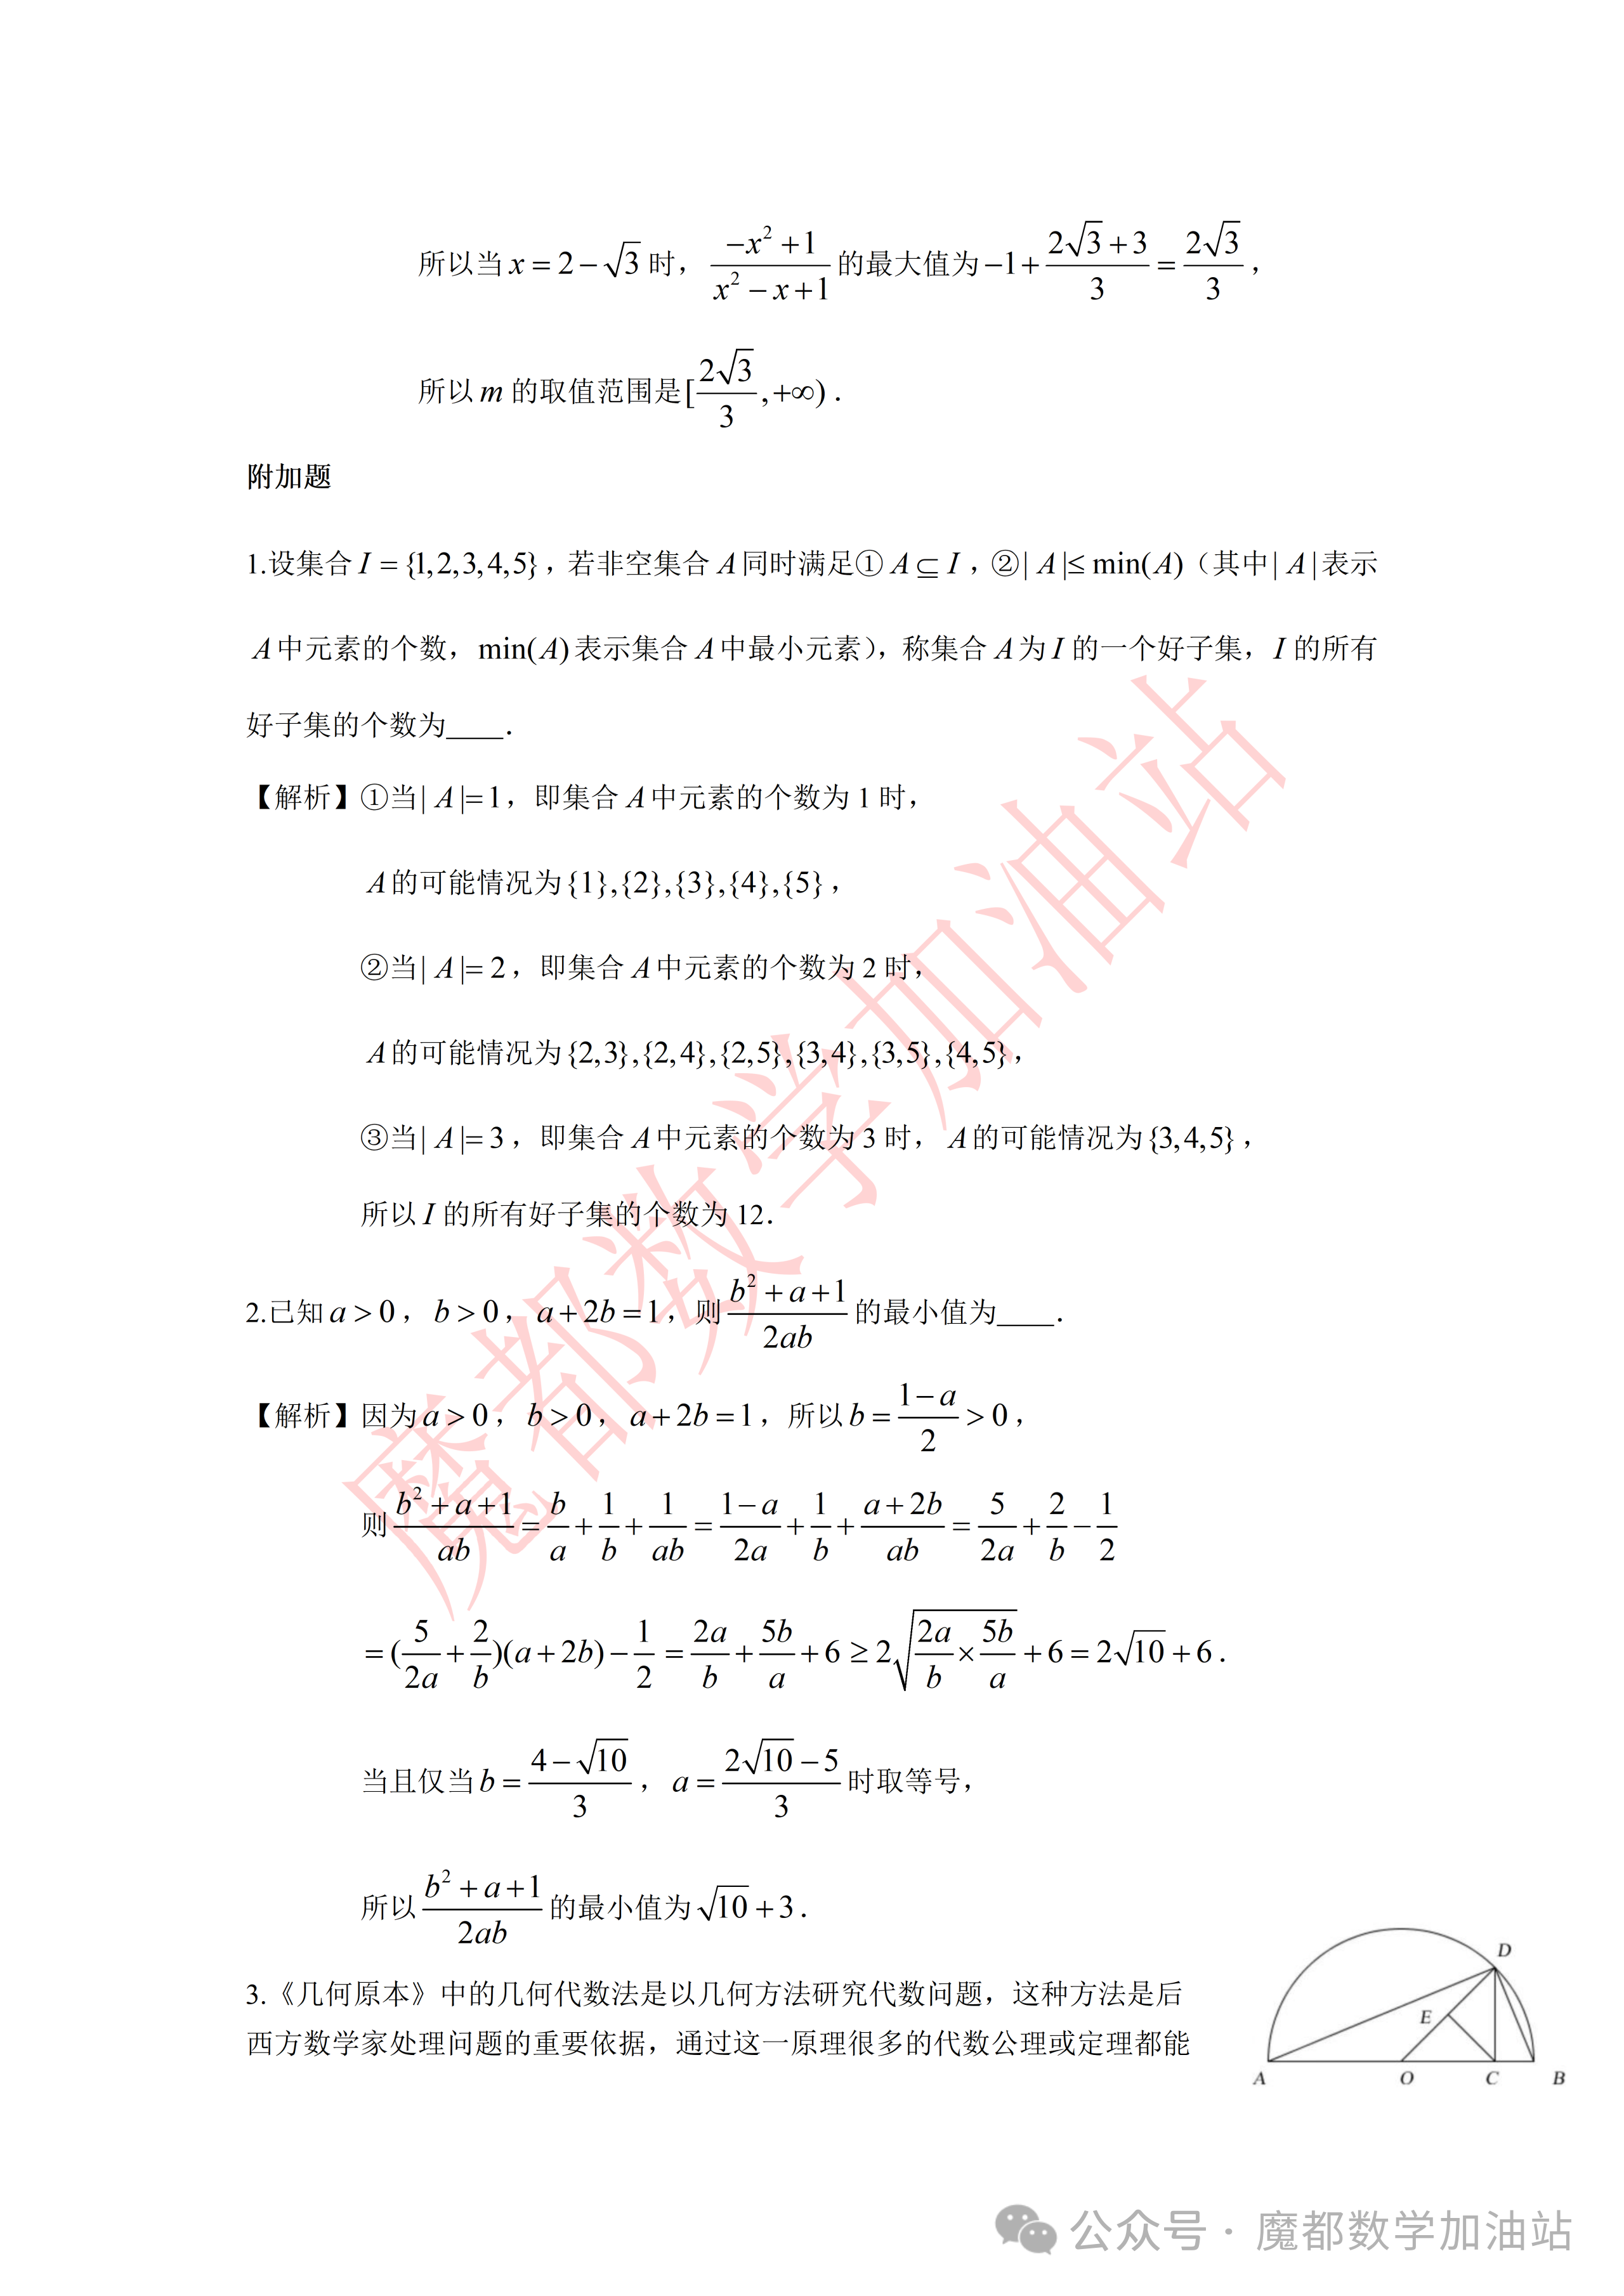
\includegraphics[width=.34\linewidth,trim=1960bp 310bp 90bp 3015bp,clip]{../原图/高一47_七宝中学_抱孩子练习9.26/08.png}
\end{center}

① $\dfrac{a+b}{2}\geqslant\sqrt{ab}$（$a>0$，$b>0$）；
② $a^2+b^2\geqslant2ab$（$a>0$，$b>0$）；
③ $\sqrt{ab}\geqslant\dfrac{2}{\dfrac1a+\dfrac1b}$（$a>0$，$b>0$）；
④ $\sqrt{\dfrac{a^2+b^2}{2}}\geqslant\dfrac{a+b}{2}$（$a>0$，$b>0$）.

\ifanswer
\solbegin
\step{因为 $AC+CB=a+b$，所以 $OD=\dfrac{AB}{2}=\dfrac{AC+CB}{2}=\dfrac{a+b}{2}$；}
\step{由射影定理得 $CD=\sqrt{AC\times CB}=\sqrt{ab}$，又因为 $OD\geqslant CD$，}
\step{所以 $\dfrac{a+b}{2}\geqslant\sqrt{ab}$，故①正确；}
\step{由射影定理得 $CD^2=DE\times OD$，所以 $DE=\dfrac{CD^2}{OD}=\dfrac{ab}{\dfrac{a+b}{2}}=\dfrac{2}{\dfrac1a+\dfrac1b}$，}
\step{又因为 $CD\geqslant DE$，所以 $\sqrt{ab}\geqslant\dfrac{2}{\dfrac1a+\dfrac1b}$，故③正确；}
\step{故该图形可以完成的所有无字证明为①③.}
\solend

\fi

% 注：原卷此处印作等式 $|x^2+a|+|x-a|=|x^2+x|$（在 $x>0$ 时与三角不等式下界等价），本稿曾改写成
% 不等式，现按原卷照录（原卷如此，照录未改）。
\item 若对任意 $x\in[2,3]$，均有 $|x^2+a|+|x-a|=|x^2+x|$，则实数 $a$ 的取值范围为 \blankline[4.4em].

\ifanswer
\solbegin
\step{因为 $|a|+|b|=|a+b|$ 当且仅当 $ab\geqslant0$ 时取等号，}
\step{所以 $(x^2+a)(x-a)\geqslant0$，即 $(a+x^2)(a-x)\leqslant0$，所以 $-x^2\leqslant a\leqslant x$ 恒成立，}
\step{因为 $x\in[2,3]$，所以 $-4\leqslant a\leqslant2$，所以实数 $a$ 的取值范围为 $[-4,2]$.}
\solend

\fi

\end{enumerate}

\end{document}
"
%
% 原始材料是微信公众号图文（公众号“魔都数学加油站”连载“27学年高一47”，署名“破晓”，
% 2026-10-02 17:56 发布，原文标题“27学年高一47——2026-2027年上海市七宝中学高一上抱孩子练习9.26”，
% 原文链接 https://mp.weixin.qq.com/s/mhkyDwjn7QFP_Z_NOcPkQA），正文为 9 张 PNG 页。
% 第 1—7、9 页分辨率为 4762×6735，第 8 页为 2560×3620；均按原图逐页核对。
% 原卷文字、选项、答案与解析均照录；粉色斜水印及灰色公众号页脚属水印/页脚，未录入。
%
% 卷首标题：原卷印作“2026-2027 年七宝中学高一上抱孩子练习 9.26”（公众号标题里的“上海市”
% 三字卷面标题行没有，本稿照卷面），年份区间按全稿惯例排 en dash，作业名保留原卷日期“9.26”。
% 原卷未印独立副标题；本稿按“知识模块”口径补出“集合与常用逻辑用语、不等式”。
%
% 与原卷的排版差异：
%   ① 原卷分“一、填空题”“二、选择题”“三、解答题”“附加题”四节；前三节题号为 3—16，
%      分别有 8 道填空、3 道选择、3 道解答；附加题另起 1—4 编号；
%   ② 原卷题下直接印答案/解析，本稿按全稿统一收进答案版；填空横线采用统一长度；
%   ③ 原卷未印副标题，本稿按“知识模块”口径补出（见卷首标题）；
%   ④ 全卷只有附加题第 3 题带图，直接从原卷第 8 页裁取。
%
% 原卷存疑（照录未改，见源码中该处上方注释）：
%   ① 第 9 题集合 C 的条件原文作“C={x|y=..., x 是整数}”，其中 y 未在集合描述中定义；
%      本稿照录原记号，未代换为 x。
%   ② 附加题第 3 题原文作“后西方数学家”，措辞存疑（疑漏“世”字）；本稿照录未改。
%
\documentclass[a4paper,11pt]{article}
\usepackage{common}

\begin{document}

\examtitlest[3]{2026--2027 年七宝中学高一上抱孩子练习 9.26}{集合与常用逻辑用语、不等式}

\bigsec{一、填空题}

\begin{enumerate}
\setcounter{enumi}{2}

\item 若不等式 $|x|<a$ 的一个充分条件为 $0<x<1$，则实数 $a$ 的取值范围是 \blankline[4.4em].

\ifanswer
\solbegin
\step{由 $|x|<a$ 得到 $-a<x<a$，}
\step{又不等式 $|x|<a$ 的一个充分条件为 $0<x<1$，所以 $a\geqslant1$.}
\solend

\fi

\item 已知命题“$\exists x\in\R$，使 $4x^2+(a-2)x+\dfrac14=0$”是假命题，则实数 $a$ 的取值范围是 \blankline[4.4em].

\ifanswer
\solbegin
% 注：原卷首句作“为真命题”（先按命题为真推出 $\Delta\geqslant0$，再由其为假得 $0<a<4$），原卷如此，照录未改。
\step{命题 $\exists x\in\R$，使 $4x^2+(a-2)x+\dfrac14=0$ 为真命题，}
\step{则 $\Delta=(a-2)^2-4\times4\times\dfrac14=a^2-4a\geqslant0$，解得 $a\leqslant0$ 或 $a\geqslant4$，}
\step{而命题“$\exists x\in\R$，使 $4x^2+(a-2)x+\dfrac14=0$”是假命题，则 $0<a<4$，}
\step{所以实数 $a$ 的取值范围是 $\{a\mid0<a<4\}$.}
\solend

\fi

\item 已知集合 $A=\{x\mid(a-1)x^2+3x-2=0\}$ 有且仅有两个子集，则实数 $a=$ \blankline[4.4em].

\ifanswer
\solbegin
\step{集合 $A=\{x\mid(a-1)x^2+3x-2=0\}$ 有且仅有两个不同的子集，}
\step{所以 $a-1=0$ 或 $\begin{cases}a-1\neq0\\\Delta=9+8(a-1)=0\end{cases}$，解得实数 $a=1$ 或 $a=-\dfrac18$.}
\solend

\fi

\item 已知函数 $y=x^2+bx+3$（其中 $b$ 是实数）中，$y$ 的取值范围是 $[0,+\infty)$，若关于 $x$ 的不等式 $x^2+bx+3<c$ 的解集为 $m-8<x<m$，则实数 $c$ 的值为 \blankline[4.4em].

\ifanswer
\solbegin
\step{因为 $y$ 的取值范围是 $[0,+\infty)$，所以 $\Delta=b^2-12=0$，解得 $b^2=12$，}
\step{因为不等式 $x^2+bx+3<c$ 的解集为 $m-8<x<m$，}
\step{令 $x^2+bx+3=c$，即 $x^2+bx+3-c=0$，方程的两根为 $x_1=m-8$，$x_2=m$，}
\step{所以 $|x_2-x_1|=\sqrt{(x_1+x_2)^2-4x_1x_2}=\sqrt{b^2-4(3-c)}=8$，即 $\sqrt{12-4(3-c)}=8$，}
\step{且判别式 $\Delta=b^2-4(3-c)=12-4(3-c)>0$，解得 $c=16$.}
\solend

\fi

\item 关于 $x$ 的不等式 $|x-1|+|x+1|\geqslant a$ 的解集为 $\R$，则实数 $a$ 的取值范围为 \blankline[4.4em].

\ifanswer
\solbegin
\step{因为 $|x-1|+|x+1|\geqslant|x-1-(x+1)|=2$，}
\step{若关于 $x$ 的不等式 $|x-1|+|x+1|\geqslant a$ 的解集为 $\R$，则实数 $a$ 的取值范围为 $a\leqslant2$.}
\solend

\fi

\item 已知 $m>0$，$xy>0$，当 $x+y=2$ 时，不等式 $\dfrac2x+\dfrac my\geqslant4$ 恒成立，则 $m$ 的取值范围是 \blankline[4.4em].

\ifanswer
\solbegin
\step{因为 $m>0$，$xy>0$，$x+y=2$，}
\step{所以 $\dfrac2x+\dfrac my=\dfrac12(x+y)\left(\dfrac2x+\dfrac my\right)
=\dfrac12\left(m+2+\dfrac{2y}{x}+\dfrac{mx}{y}\right)$}
\step{$\geqslant\dfrac12\left(m+2+2\sqrt{\dfrac{2y}{x}\cdot\dfrac{mx}{y}}\right)=\dfrac12\left(m+2+2\sqrt{2m}\right)$，}
\step{当且仅当 $\dfrac{2y}{x}=\dfrac{mx}{y}$，即 $y^2=\dfrac{mx^2}{2}$ 时取等号.}
\step{因为不等式 $\dfrac2x+\dfrac my\geqslant4$ 恒成立，所以 $\dfrac12(m+2+2\sqrt{2m})\geqslant4$，}
\step{整理得 $(\sqrt m+3\sqrt2)(\sqrt m-\sqrt2)\geqslant0$，解得 $\sqrt m\geqslant\sqrt2$，即 $m\geqslant2$，}
\step{所以 $m$ 的取值范围为 $[2,+\infty)$.}
\solend

\fi

\item 已知全集为 $\R$，集合 $D=\{x\mid x^2-ax+a^2-19=0\}$，
$B=\{y\mid y=-x^2+2x+2,\ y\text{ 是正整数}\}$，
% 注：本题集合 C 的条件原文作“C={x|y=..., x 是整数}”，其中 y 未在集合描述中定义；照录未改。
集合 $C=\left\{x\mathrel{\Big|}y=\sqrt{\dfrac{2-x}{x+1}},\ x\text{ 是整数}\right\}$，且集合 $D$ 满足 $D\cap B\neq\varnothing$，$\overline{D}\cup\overline{C}=\R$，则实数 $a$ 的值是 \blankline[4.4em].

\ifanswer
\solbegin
\step{集合 $B=\{y\mid y=-x^2+2x+2,\ y\text{ 是正整数}\}=\{1,2,3\}$，}
\step{集合 $C=\left\{x\mathrel{\Big|}y=\sqrt{\dfrac{2-x}{x+1}},\ x\text{ 是整数}\right\}=\{0,1,2\}$，}
\step{集合 $D=\{x\mid x^2-ax+a^2-19=0\}$ 且集合 $D$ 满足 $D\cap B\neq\varnothing$，$\overline{D}\cup\overline{C}=\R$，}
\step{所以 $3\in D$，解得 $a=5$ 或 $a=-2$，}
\step{经检验，$a=5$ 不符合 $\overline{D}\cup\overline{C}=\R$，舍去，$a=-2$ 满足题意，即 $a=-2$.}
\solend

\fi

% 注：本题解析中，$a=\pm2\sqrt2$ 时 $B$ 的二重根按 $-\dfrac a2$ 应为 $\mp\sqrt2$，原卷印作 $\mp2\sqrt2$、
% $-\dfrac{3\sqrt2}4$，$C(B)=3$ 的计算也随之按原卷保留（原卷如此，照录未改）。
\item 用 $C(A)$ 表示非空集合 $A$ 中的元素的个数，定义 $A*B=|C(A)-C(B)|$，已知集合 $A$ 有三个真子集，
$B=\{x\mid(ax^2+3x)(x^2+ax+2)=0,\ x\in\R\}$，若 $A*B=1$，设实数 $a$ 所有可能取值构成集合 $S$，则 $C(S)=$ \blankline[4.4em].

\ifanswer
\solbegin
\step{集合 $A$ 有三个真子集，则集合 $A$ 中有 $2$ 个元素，则 $C(A)=2$，}
\step{由 $A*B=1$，得 $C(B)=1$ 或 $3$，}
\step{即方程 $(ax^2+3x)\cdot(x^2+ax+2)=0$ 有一个根或 $3$ 个根；}
\step{若 $(ax^2+3x)\cdot(x^2+ax+2)=0$，则必有 $ax^2+3x=0$ 或 $x^2+ax+2=0$，}
\step{若 $ax^2+3x=0$，则 $x=0$ 或 $ax+3=0$，}
\step{当 $a=0$ 时，$B=\{0\}$，$C(B)=1$，符合题意；}
\step{当 $a\neq0$ 时，$ax^2+3x=0$ 对应的根为 $0$ 和 $-\dfrac3a$；}
\step{故①需 $x^2+ax+2=0$ 有两等根且根不为 $0$ 和 $-\dfrac3a$，}
\step{当 $\Delta=0$ 时，$a=\pm2\sqrt2$，}
\step{$a=2\sqrt2$，此时 $B=\left\{0,-2\sqrt2,-\dfrac{3\sqrt2}{4}\right\}$，$C(B)=3$，符合题意；}
\step{$a=-2\sqrt2$，此时 $B=\left\{0,2\sqrt2,\dfrac{3\sqrt2}{4}\right\}$，$C(B)=3$，符合题意；}
\step{②当 $-\dfrac3a$ 是 $x^2+ax+2=0$ 的根时，解得 $a=\pm3$；}
\step{$a=3$，此时 $B=\{0,-1,-2\}$，$C(B)=3$，符合题意；}
\step{$a=-3$，此时 $B=\{0,1,2\}$，$C(B)=3$，符合题意；}
\step{综上，$a$ 可取的值为 $0$、$\pm3$、$\pm2\sqrt2$，则 $C(S)=5$.}
\solend

\fi

\end{enumerate}

\bigsec{二、选择题}

\begin{enumerate}
\setcounter{enumi}{10}

\item 已知集合 $A=\left\{x\mathrel{\Big|}\dfrac1x<1\right\}$，$B=\{x\mid x^2-2x-3\leqslant0\}$，则 $A\cap B=$\mbox{（\quad）}

\keepwithprev
A. $\{x\mid1<x\leqslant3\}$\qquad B. $\{x\mid1\leqslant x\leqslant3\text{ 或 }-1\leqslant x<0\}$

C. $\{x\mid-1\leqslant x<0\}$\qquad D. $\{x\mid1<x\leqslant3\text{ 或 }-1\leqslant x<0\}$

\ans{$D$}

% 注：原卷本题只有题干＋选项（答案印在括号内），没有解析；此处照录原卷的"无解析"状态，不排解析。
\item 使 $x(y-2)=0$ 成立的一个充分条件是\mbox{（\quad）}

\keepwithprev
A. $x^2+(y-2)^2=0$\qquad B. $(x-2)^2+y^2=0$

C. $x^2+y^2=1$\qquad D. $x+y-2=0$

\ans{$A$}

\ifanswer
\solbegin
\step{对于 $A$：若 $x^2+(y-2)^2=0$，则 $x=0$ 且 $y=2$，此时 $x(y-2)=0$ 成立，}
\step{即充分性成立.}
\step{若 $x(y-2)=0$，则 $x=0$ 或 $y=2$，当 $x=0$，$y=3$ 时，$x^2+(y-2)^2=0$ 不成立，}
\step{即必要性不成立，}
\step{故 $x^2+(y-2)^2=0$ 是 $x(y-2)=0$ 成立的充分不必要条件；}
\step{对于 $B$：$(x-2)^2+y^2=0$，则 $x=2$ 且 $y=0$，此时 $x(y-2)=0$ 不成立，}
\step{即充分性不成立；}
\step{对于 $C$：$x^2+y^2=1$，此时 $x(y-2)=0$ 不一定成立，即充分性不成立；}
\step{对于 $D$：$x+y-2=0$，此时 $x(y-2)=0$ 不一定成立，即充分性不成立.}
\step{故选 $A$.}
\solend

\fi

\item 已知 $a$、$b$、$c\in\R$，若关于 $x$ 的不等式 $0\leqslant x+\dfrac ax+b\leqslant\dfrac cx-1$ 的解集为 $[x_1,x_2]\cup\{x_3\}$（$x_3>x_2>x_1>0$），则\mbox{（\quad）}

\keepwithprev
A. 不存在有序数组 $(a,b,c)$，使得 $x_2-x_1=1$

B. 存在唯一有序数组 $(a,b,c)$，使得 $x_2-x_1=1$

C. 有且只有两组有序数组 $(a,b,c)$，使得 $x_2-x_1=1$

D. 存在无穷多组有序数组 $(a,b,c)$，使得 $x_2-x_1=1$

\ans{$D$}

\ifanswer
\solbegin
\step{因为不等式 $0\leqslant x+\dfrac ax+b\leqslant\dfrac cx-1$ 的解集为 $[x_1,x_2]\cup\{x_3\}$（$x_3>x_2>x_1>0$），}
\step{所以 $0\leqslant x^2+bx+a\leqslant c-x$ 在 $[x_1,x_2]\cup\{x_3\}$ 上成立，}
\step{假设 $x_1=m$，$x_2=m+1$，$x_3=n$，}
\step{则 $c-n=0=n^2+bn+a$，由 $x_3$ 为一个独立的数得出，}
\step{所以 $n=c$，且 $m+1$ 与 $n$ 为方程 $x^2+bx+a=0$ 的两个根，}
\step{因为 $x_3>x_2>x_1>0$，所以 $-b=m+n+1=m+c+1$，$a=mn+n=mc+c$，}
\step{所以 $b=-m-c-1$，}
\step{且点 $(x_1,x_1^2+bx_1+a)$ 为 $y=x^2+bx+a$ 与 $y=c-x$ 的左交点，}
\step{所以 $m^2+bm+a=c-m$ 且 $b=-m-c-1$，$a=mc+c$，}
% 注：原卷此行的末句作“所以 $c-m=c-m$ 恒成立”（未写成 $x_2-x_1=1$），原卷如此，照录未改。
\step{故 $m^2+bm+a=m^2-m^2-mc-m+mc+c=c-m$，所以 $c-m=c-m$ 恒成立，}
\step{所以不论 $a$、$b$、$c$ 取何值，$x_2-x_1=1$ 恒成立，}
\step{即存在无穷多组有序数组 $(a,b,c)$，使得 $x_2-x_1=1$，}
\step{故选项 $A$、$B$、$C$ 错误，选项 $D$ 正确. 故选 $D$.}
\solend

\fi

\end{enumerate}

\bigsec{三、解答题}

\begin{enumerate}
\setcounter{enumi}{13}

\item 设正实数 $x$、$y$，满足 $2x+y=1$，求：

\begin{enumerate}[label=(\arabic*)]
\item $\sqrt{2x}+\sqrt y$ 的最大值；
\item $\dfrac2x+\dfrac1y$ 的最小值.
\end{enumerate}

\ifanswer
\solbegin
\stepm{(1)}{对于 $(\sqrt{2x}+\sqrt y)^2=2x+y+2\sqrt{2xy}\leqslant1+1=2$，}
\step{当且仅当 $\sqrt{2x}=\sqrt y$ 时取等号，故 $\sqrt{2x}+\sqrt y$ 的最大值为 $\sqrt2$；}
\stepm{(2)}{$\dfrac2x+\dfrac1y=\left(\dfrac2x+\dfrac1y\right)(2x+y)=5+\dfrac{2y}{x}+\dfrac{2x}{y}\geqslant5+4=9$，}
\step{当且仅当 $\dfrac{2y}{x}=\dfrac{2x}{y}$，即 $x=y=\dfrac13$ 时取等号，故 $\dfrac2x+\dfrac1y$ 的最小值为 $9$.}
\solend

\fi

\ansspace[6]

\item 设 $x_1$、$x_2$ 为关于 $x$ 的方程 $x^2-2(m+2)x+m^2-1=0$ 的两实数根.

\begin{enumerate}[label=(\arabic*)]
\item 若 $x_1$、$x_2$ 满足 $x_1^2+x_2^2=18$，试求 $m$ 的值；
\item 若 $x_1$、$x_2$ 均大于 $0$，求 $m$ 的取值范围.
\end{enumerate}

\ifanswer
\solbegin
\stepm{(1)}{由 $\Delta=4(m+2)^2-4(m^2-1)\geqslant0$，解得 $m\geqslant-\dfrac54$，}
\step{由韦达定理得 $x_1+x_2=2(m+2)$，$x_1x_2=m^2-1$，}
\step{又 $x_1^2+x_2^2=(x_1+x_2)^2-2x_1x_2=4(m+2)^2-2(m^2-1)=18$，}
\step{即 $m^2+8m=0$，解得 $m=0$ 或 $m=-8$（舍），故 $m$ 的值为 $0$；}
% 注：原卷此处作“由（2）得”（对照上一小问，所指应为（1）），原卷如此，照录未改。
\stepm{(2)}{由（2）得 $m\geqslant-\dfrac54$，}
\step{又 $x_1$、$x_2$ 均大于 $0$，则 $\begin{cases}2(m+2)>0\\m^2-1>0\end{cases}$，解得 $\begin{cases}m>-2\\m>1\text{或}m<-1\end{cases}$，}
\step{综上，实数 $m$ 的取值范围为 $\left[-\dfrac54,-1\right)\cup(1,+\infty)$.}
\solend

\fi

\ansspace[6]

\item 已知函数 $f(x)=(m+1)x^2-mx+m-1$（$m\in\R$）.

\begin{enumerate}[label=(\arabic*)]
\item 若不等式 $f(x)<0$ 的解集是空集，求 $m$ 的取值范围；
\item 当 $m>-2$ 时，解不等式 $f(x)\geqslant m$；
\item 若不等式 $f(x)\geqslant0$ 的解集为 $D$，若 $[-1,1]\subseteq D$，求 $m$ 的取值范围.
\end{enumerate}

\ifanswer
\solbegin
\stepm{(1)}{①当 $m+1=0$，即 $m=-1$ 时，$f(x)=x-2$，不合题意；}
\step{②当 $m+1\neq0$，即 $m\neq-1$ 时，$\begin{cases}m+1>0\\\Delta=m^2-4(m+1)(m-1)\leqslant0\end{cases}$，解得 $m\geqslant\dfrac{2\sqrt3}{3}$，}
\step{所以 $m$ 的取值范围是 $\left[\dfrac{2\sqrt3}{3},+\infty\right)$；}
\stepm{(2)}{因为 $f(x)\geqslant m$，所以 $(m+1)x^2-mx-1\geqslant0$，即 $[(m+1)x+1](x-1)\geqslant0$，}
\step{①当 $m+1=0$ 即 $m=-1$ 时，不等式的解集为 $[1,+\infty)$；}
\step{②当 $m+1>0$ 即 $m>-1$ 时，$\left(x+\dfrac1{m+1}\right)(x-1)\geqslant0$，}
\step{因为 $-\dfrac1{m+1}<0$，所以不等式的解集为 $\left(-\infty,-\dfrac1{m+1}\right]\cup[1,+\infty)$；}
\step{③当 $m+1<0$ 即 $-2<m<-1$ 时，$\left(x+\dfrac1{m+1}\right)(x-1)\leqslant0$，}
\step{因为 $-2<m<-1$，所以 $-1<m+1<0$，所以 $-\dfrac1{m+1}>1$，}
\step{所以不等式的解集为 $\left[1,-\dfrac1{m+1}\right]$；}
\stepm{(3)}{不等式 $f(x)\geqslant0$ 的解集为 $D$，若 $[-1,1]\subseteq D$，}
\step{即对任意的 $x\in[-1,1]$，不等式 $(m+1)x^2-mx+m-1\geqslant0$ 恒成立，}
\step{即 $m(x^2-x+1)\geqslant-x^2+1$ 恒成立，}
\step{因为 $x^2-x+1>0$ 恒成立，所以 $m\geqslant\dfrac{-x^2+1}{x^2-x+1}=-1+\dfrac{2-x}{x^2-x+1}$ 恒成立，}
\step{设 $t=2-x$，则 $t\in[1,3]$，$x=2-t$，}
\step{则 $\dfrac{2-x}{x^2-x+1}=\dfrac{t}{(2-t)^2-(2-t)+1}=\dfrac{t}{t^2-3t+3}=\dfrac1{t+\dfrac3t-3}$，}
\step{因为 $t+\dfrac3t\geqslant2\sqrt3$，当且仅当 $t=\sqrt3$ 时取等号，}
\step{所以 $\dfrac{2-x}{x^2-x+1}\leqslant\dfrac1{2\sqrt3-3}=\dfrac{2\sqrt3+3}{3}$，当且仅当 $x=2-\sqrt3$ 时取等号，}
\step{所以当 $x=2-\sqrt3$ 时，$\dfrac{-x^2+1}{x^2-x+1}$ 的最大值为 $-1+\dfrac{2\sqrt3+3}{3}=\dfrac{2\sqrt3}{3}$，}
\step{所以 $m$ 的取值范围是 $\left[\dfrac{2\sqrt3}{3},+\infty\right)$.}
\solend

\fi

\ansspace[8]

\end{enumerate}

\bigsec{附加题}

\begin{enumerate}

\item 设集合 $I=\{1,2,3,4,5\}$，若非空集合 $A$ 同时满足① $A\subseteq I$，② $|A|\leqslant\min(A)$（其中 $|A|$ 表示集合 $A$ 中元素的个数，$\min(A)$ 表示集合 $A$ 中最小元素），称集合 $A$ 为 $I$ 的一个好子集，$I$ 所有好子集的个数为 \blankline[4.4em].

\ifanswer
\solbegin
\step{①当 $|A|=1$，即集合 $A$ 中元素的个数为 $1$ 时，}
\step{$A$ 的可能情况为 $\{1\}$、$\{2\}$、$\{3\}$、$\{4\}$、$\{5\}$，}
\step{②当 $|A|=2$，即集合 $A$ 中元素的个数为 $2$ 时，}
\step{$A$ 的可能情况为 $\{2,3\}$、$\{2,4\}$、$\{2,5\}$、$\{3,4\}$、$\{3,5\}$、$\{4,5\}$，}
\step{③当 $|A|=3$，即集合 $A$ 中元素的个数为 $3$ 时，$A$ 的可能情况为 $\{3,4,5\}$，}
\step{所以 $I$ 的所有好子集的个数为 $12$.}
\solend

\fi

\item 已知 $a>0$，$b>0$，$a+2b=1$，则 $\dfrac{b^2+a+1}{2ab}$ 的最小值为 \blankline[4.4em].

\ifanswer
\solbegin
\step{因为 $a>0$，$b>0$，$a+2b=1$，所以 $b=\dfrac{1-a}{2}>0$，}
\step{则 $\dfrac{b^2+a+1}{ab}=\dfrac ba+\dfrac1b+\dfrac1{ab}=\dfrac{1-a}{2a}+\dfrac1b+\dfrac{a+2b}{ab}=\dfrac5{2a}+\dfrac2b-\dfrac12$}
\step{$=\left(\dfrac5{2a}+\dfrac2b\right)(a+2b)-\dfrac12=\dfrac{2a}{b}+\dfrac{5b}{a}+6\geqslant2\sqrt{\dfrac{2a}{b}\times\dfrac{5b}{a}}+6=2\sqrt{10}+6$.}
\step{当且仅当 $b=\dfrac{4-\sqrt{10}}{3}$，$a=\dfrac{2\sqrt{10}-5}{3}$ 时取等号，}
\step{所以 $\dfrac{b^2+a+1}{2ab}$ 的最小值为 $\sqrt{10}+3$.}
\solend

\fi

% 注：本题原文作“后西方数学家”，措辞存疑（疑漏“世”字）；照录未改，见文件头“原卷存疑”②。
% 又原文作"很多的代数公理或定理都能够通过图形实现证明"（"公理"疑为"公式"笔误）、
% "连结 OD,AD,BD"，均原卷如此，照录未改。
\item 《几何原本》中的几何代数法是以几何方法研究代数问题，这种方法是后西方数学家处理问题的重要依据，通过这一原理很多的代数公理或定理都能够通过图形实现证明，也称之为无字证明，现有图形如图所示，$C$ 为线段 $AB$ 上的点，且 $AC=a$，$BC=b$，$O$ 为 $AB$ 的中点，以 $AB$ 为直径作半圆，过点 $C$ 作 $AB$ 的垂线交半圆于 $D$，连结 $OD,AD,BD$，过点 $C$ 作 $OD$ 的垂线，垂足为 $E$，若不添加辅助线，则该图形可以完成的所有无字证明为 \blankline[4.4em]（填写序号）.

\begin{center}
% 插图直接裁自原卷第 8 页，未重绘；用 trim/clip 保留原图与标注。
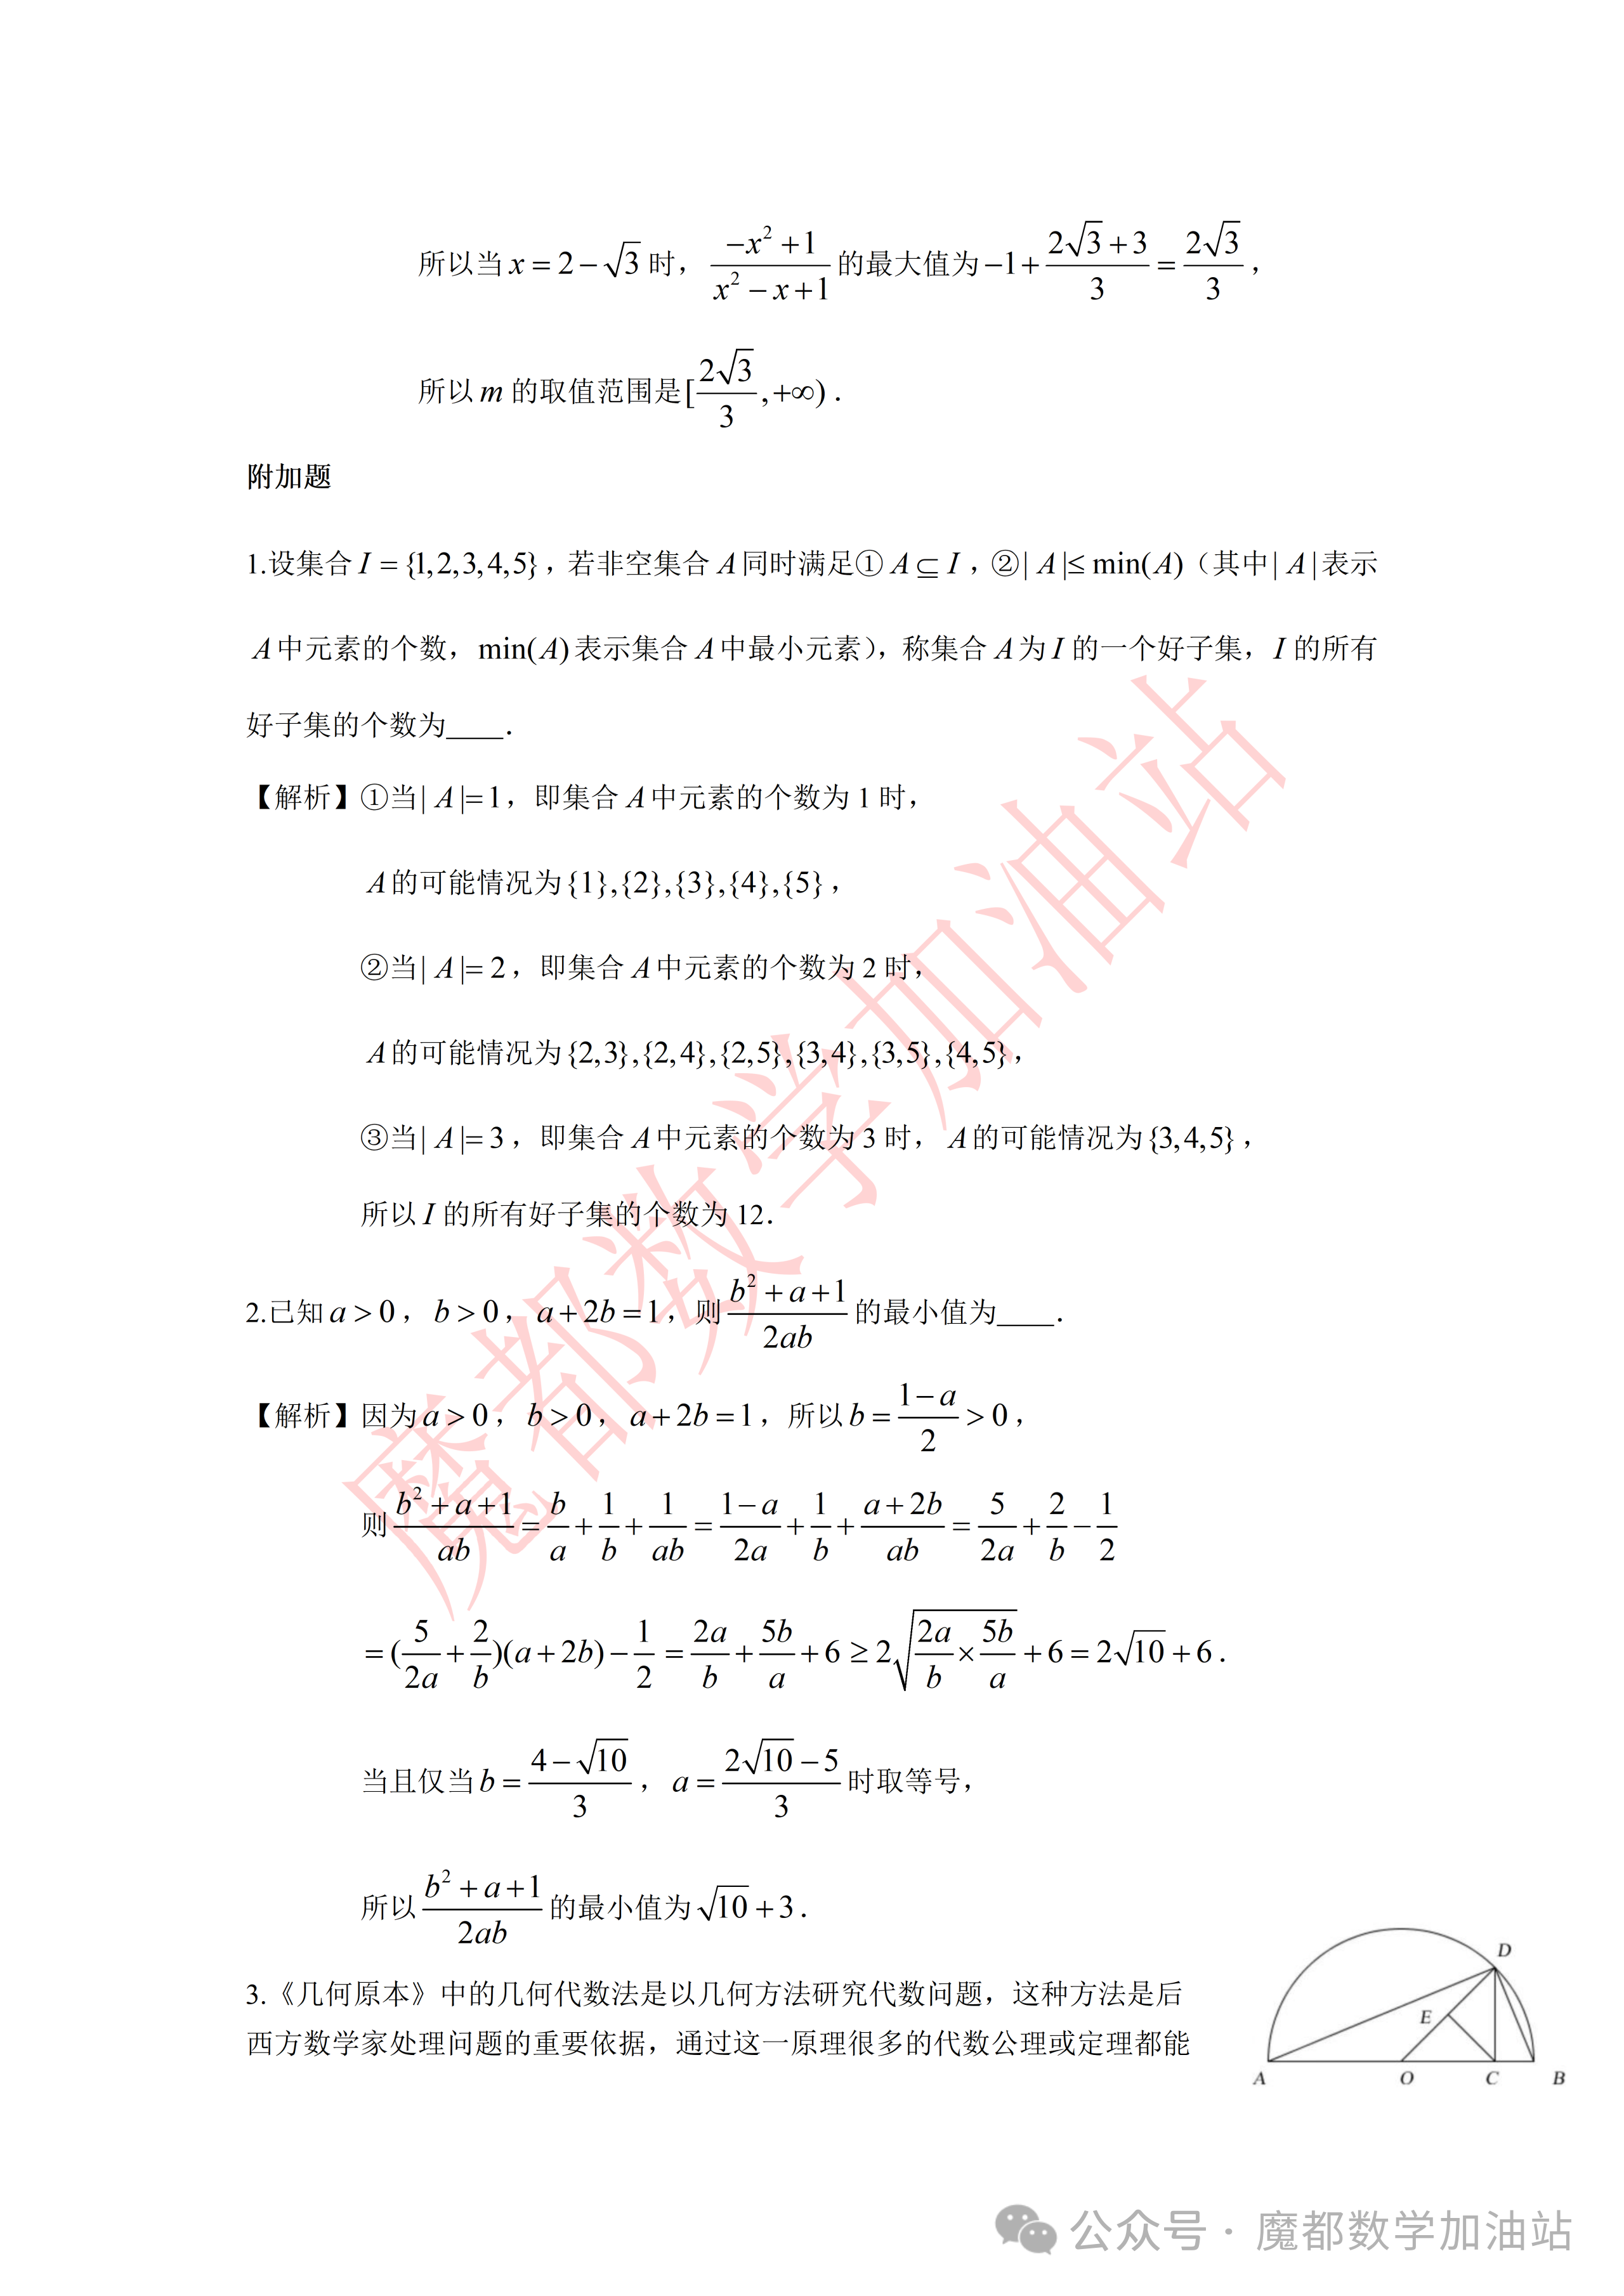
\includegraphics[width=.34\linewidth,trim=1960bp 310bp 90bp 3015bp,clip]{../原图/高一47_七宝中学_抱孩子练习9.26/08.png}
\end{center}

① $\dfrac{a+b}{2}\geqslant\sqrt{ab}$（$a>0$，$b>0$）；
② $a^2+b^2\geqslant2ab$（$a>0$，$b>0$）；
③ $\sqrt{ab}\geqslant\dfrac{2}{\dfrac1a+\dfrac1b}$（$a>0$，$b>0$）；
④ $\sqrt{\dfrac{a^2+b^2}{2}}\geqslant\dfrac{a+b}{2}$（$a>0$，$b>0$）.

\ifanswer
\solbegin
\step{因为 $AC+CB=a+b$，所以 $OD=\dfrac{AB}{2}=\dfrac{AC+CB}{2}=\dfrac{a+b}{2}$；}
\step{由射影定理得 $CD=\sqrt{AC\times CB}=\sqrt{ab}$，又因为 $OD\geqslant CD$，}
\step{所以 $\dfrac{a+b}{2}\geqslant\sqrt{ab}$，故①正确；}
\step{由射影定理得 $CD^2=DE\times OD$，所以 $DE=\dfrac{CD^2}{OD}=\dfrac{ab}{\dfrac{a+b}{2}}=\dfrac{2}{\dfrac1a+\dfrac1b}$，}
\step{又因为 $CD\geqslant DE$，所以 $\sqrt{ab}\geqslant\dfrac{2}{\dfrac1a+\dfrac1b}$，故③正确；}
\step{故该图形可以完成的所有无字证明为①③.}
\solend

\fi

% 注：原卷此处印作等式 $|x^2+a|+|x-a|=|x^2+x|$（在 $x>0$ 时与三角不等式下界等价），本稿曾改写成
% 不等式，现按原卷照录（原卷如此，照录未改）。
\item 若对任意 $x\in[2,3]$，均有 $|x^2+a|+|x-a|=|x^2+x|$，则实数 $a$ 的取值范围为 \blankline[4.4em].

\ifanswer
\solbegin
\step{因为 $|a|+|b|=|a+b|$ 当且仅当 $ab\geqslant0$ 时取等号，}
\step{所以 $(x^2+a)(x-a)\geqslant0$，即 $(a+x^2)(a-x)\leqslant0$，所以 $-x^2\leqslant a\leqslant x$ 恒成立，}
\step{因为 $x\in[2,3]$，所以 $-4\leqslant a\leqslant2$，所以实数 $a$ 的取值范围为 $[-4,2]$.}
\solend

\fi

\end{enumerate}

\end{document}
"
%
% 原始材料是微信公众号图文（公众号“魔都数学加油站”连载“27学年高一47”，署名“破晓”，
% 2026-10-02 17:56 发布，原文标题“27学年高一47——2026-2027年上海市七宝中学高一上抱孩子练习9.26”，
% 原文链接 https://mp.weixin.qq.com/s/mhkyDwjn7QFP_Z_NOcPkQA），正文为 9 张 PNG 页。
% 第 1—7、9 页分辨率为 4762×6735，第 8 页为 2560×3620；均按原图逐页核对。
% 原卷文字、选项、答案与解析均照录；粉色斜水印及灰色公众号页脚属水印/页脚，未录入。
%
% 卷首标题：原卷印作“2026-2027 年七宝中学高一上抱孩子练习 9.26”（公众号标题里的“上海市”
% 三字卷面标题行没有，本稿照卷面），年份区间按全稿惯例排 en dash，作业名保留原卷日期“9.26”。
% 原卷未印独立副标题；本稿按“知识模块”口径补出“集合与常用逻辑用语、不等式”。
%
% 与原卷的排版差异：
%   ① 原卷分“一、填空题”“二、选择题”“三、解答题”“附加题”四节；前三节题号为 3—16，
%      分别有 8 道填空、3 道选择、3 道解答；附加题另起 1—4 编号；
%   ② 原卷题下直接印答案/解析，本稿按全稿统一收进答案版；填空横线采用统一长度；
%   ③ 原卷未印副标题，本稿按“知识模块”口径补出（见卷首标题）；
%   ④ 全卷只有附加题第 3 题带图，直接从原卷第 8 页裁取。
%
% 原卷存疑（照录未改，见源码中该处上方注释）：
%   ① 第 9 题集合 C 的条件原文作“C={x|y=..., x 是整数}”，其中 y 未在集合描述中定义；
%      本稿照录原记号，未代换为 x。
%   ② 附加题第 3 题原文作“后西方数学家”，措辞存疑（疑漏“世”字）；本稿照录未改。
%
\documentclass[a4paper,11pt]{article}
\usepackage{common}

\begin{document}

\examtitlest[3]{2026--2027 年七宝中学高一上抱孩子练习 9.26}{集合与常用逻辑用语、不等式}

\bigsec{一、填空题}

\begin{enumerate}
\setcounter{enumi}{2}

\item 若不等式 $|x|<a$ 的一个充分条件为 $0<x<1$，则实数 $a$ 的取值范围是 \blankline[4.4em].

\ifanswer
\solbegin
\step{由 $|x|<a$ 得到 $-a<x<a$，}
\step{又不等式 $|x|<a$ 的一个充分条件为 $0<x<1$，所以 $a\geqslant1$.}
\solend

\fi

\item 已知命题“$\exists x\in\R$，使 $4x^2+(a-2)x+\dfrac14=0$”是假命题，则实数 $a$ 的取值范围是 \blankline[4.4em].

\ifanswer
\solbegin
% 注：原卷首句作“为真命题”（先按命题为真推出 $\Delta\geqslant0$，再由其为假得 $0<a<4$），原卷如此，照录未改。
\step{命题 $\exists x\in\R$，使 $4x^2+(a-2)x+\dfrac14=0$ 为真命题，}
\step{则 $\Delta=(a-2)^2-4\times4\times\dfrac14=a^2-4a\geqslant0$，解得 $a\leqslant0$ 或 $a\geqslant4$，}
\step{而命题“$\exists x\in\R$，使 $4x^2+(a-2)x+\dfrac14=0$”是假命题，则 $0<a<4$，}
\step{所以实数 $a$ 的取值范围是 $\{a\mid0<a<4\}$.}
\solend

\fi

\item 已知集合 $A=\{x\mid(a-1)x^2+3x-2=0\}$ 有且仅有两个子集，则实数 $a=$ \blankline[4.4em].

\ifanswer
\solbegin
\step{集合 $A=\{x\mid(a-1)x^2+3x-2=0\}$ 有且仅有两个不同的子集，}
\step{所以 $a-1=0$ 或 $\begin{cases}a-1\neq0\\\Delta=9+8(a-1)=0\end{cases}$，解得实数 $a=1$ 或 $a=-\dfrac18$.}
\solend

\fi

\item 已知函数 $y=x^2+bx+3$（其中 $b$ 是实数）中，$y$ 的取值范围是 $[0,+\infty)$，若关于 $x$ 的不等式 $x^2+bx+3<c$ 的解集为 $m-8<x<m$，则实数 $c$ 的值为 \blankline[4.4em].

\ifanswer
\solbegin
\step{因为 $y$ 的取值范围是 $[0,+\infty)$，所以 $\Delta=b^2-12=0$，解得 $b^2=12$，}
\step{因为不等式 $x^2+bx+3<c$ 的解集为 $m-8<x<m$，}
\step{令 $x^2+bx+3=c$，即 $x^2+bx+3-c=0$，方程的两根为 $x_1=m-8$，$x_2=m$，}
\step{所以 $|x_2-x_1|=\sqrt{(x_1+x_2)^2-4x_1x_2}=\sqrt{b^2-4(3-c)}=8$，即 $\sqrt{12-4(3-c)}=8$，}
\step{且判别式 $\Delta=b^2-4(3-c)=12-4(3-c)>0$，解得 $c=16$.}
\solend

\fi

\item 关于 $x$ 的不等式 $|x-1|+|x+1|\geqslant a$ 的解集为 $\R$，则实数 $a$ 的取值范围为 \blankline[4.4em].

\ifanswer
\solbegin
\step{因为 $|x-1|+|x+1|\geqslant|x-1-(x+1)|=2$，}
\step{若关于 $x$ 的不等式 $|x-1|+|x+1|\geqslant a$ 的解集为 $\R$，则实数 $a$ 的取值范围为 $a\leqslant2$.}
\solend

\fi

\item 已知 $m>0$，$xy>0$，当 $x+y=2$ 时，不等式 $\dfrac2x+\dfrac my\geqslant4$ 恒成立，则 $m$ 的取值范围是 \blankline[4.4em].

\ifanswer
\solbegin
\step{因为 $m>0$，$xy>0$，$x+y=2$，}
\step{所以 $\dfrac2x+\dfrac my=\dfrac12(x+y)\left(\dfrac2x+\dfrac my\right)
=\dfrac12\left(m+2+\dfrac{2y}{x}+\dfrac{mx}{y}\right)$}
\step{$\geqslant\dfrac12\left(m+2+2\sqrt{\dfrac{2y}{x}\cdot\dfrac{mx}{y}}\right)=\dfrac12\left(m+2+2\sqrt{2m}\right)$，}
\step{当且仅当 $\dfrac{2y}{x}=\dfrac{mx}{y}$，即 $y^2=\dfrac{mx^2}{2}$ 时取等号.}
\step{因为不等式 $\dfrac2x+\dfrac my\geqslant4$ 恒成立，所以 $\dfrac12(m+2+2\sqrt{2m})\geqslant4$，}
\step{整理得 $(\sqrt m+3\sqrt2)(\sqrt m-\sqrt2)\geqslant0$，解得 $\sqrt m\geqslant\sqrt2$，即 $m\geqslant2$，}
\step{所以 $m$ 的取值范围为 $[2,+\infty)$.}
\solend

\fi

\item 已知全集为 $\R$，集合 $D=\{x\mid x^2-ax+a^2-19=0\}$，
$B=\{y\mid y=-x^2+2x+2,\ y\text{ 是正整数}\}$，
% 注：本题集合 C 的条件原文作“C={x|y=..., x 是整数}”，其中 y 未在集合描述中定义；照录未改。
集合 $C=\left\{x\mathrel{\Big|}y=\sqrt{\dfrac{2-x}{x+1}},\ x\text{ 是整数}\right\}$，且集合 $D$ 满足 $D\cap B\neq\varnothing$，$\overline{D}\cup\overline{C}=\R$，则实数 $a$ 的值是 \blankline[4.4em].

\ifanswer
\solbegin
\step{集合 $B=\{y\mid y=-x^2+2x+2,\ y\text{ 是正整数}\}=\{1,2,3\}$，}
\step{集合 $C=\left\{x\mathrel{\Big|}y=\sqrt{\dfrac{2-x}{x+1}},\ x\text{ 是整数}\right\}=\{0,1,2\}$，}
\step{集合 $D=\{x\mid x^2-ax+a^2-19=0\}$ 且集合 $D$ 满足 $D\cap B\neq\varnothing$，$\overline{D}\cup\overline{C}=\R$，}
\step{所以 $3\in D$，解得 $a=5$ 或 $a=-2$，}
\step{经检验，$a=5$ 不符合 $\overline{D}\cup\overline{C}=\R$，舍去，$a=-2$ 满足题意，即 $a=-2$.}
\solend

\fi

% 注：本题解析中，$a=\pm2\sqrt2$ 时 $B$ 的二重根按 $-\dfrac a2$ 应为 $\mp\sqrt2$，原卷印作 $\mp2\sqrt2$、
% $-\dfrac{3\sqrt2}4$，$C(B)=3$ 的计算也随之按原卷保留（原卷如此，照录未改）。
\item 用 $C(A)$ 表示非空集合 $A$ 中的元素的个数，定义 $A*B=|C(A)-C(B)|$，已知集合 $A$ 有三个真子集，
$B=\{x\mid(ax^2+3x)(x^2+ax+2)=0,\ x\in\R\}$，若 $A*B=1$，设实数 $a$ 所有可能取值构成集合 $S$，则 $C(S)=$ \blankline[4.4em].

\ifanswer
\solbegin
\step{集合 $A$ 有三个真子集，则集合 $A$ 中有 $2$ 个元素，则 $C(A)=2$，}
\step{由 $A*B=1$，得 $C(B)=1$ 或 $3$，}
\step{即方程 $(ax^2+3x)\cdot(x^2+ax+2)=0$ 有一个根或 $3$ 个根；}
\step{若 $(ax^2+3x)\cdot(x^2+ax+2)=0$，则必有 $ax^2+3x=0$ 或 $x^2+ax+2=0$，}
\step{若 $ax^2+3x=0$，则 $x=0$ 或 $ax+3=0$，}
\step{当 $a=0$ 时，$B=\{0\}$，$C(B)=1$，符合题意；}
\step{当 $a\neq0$ 时，$ax^2+3x=0$ 对应的根为 $0$ 和 $-\dfrac3a$；}
\step{故①需 $x^2+ax+2=0$ 有两等根且根不为 $0$ 和 $-\dfrac3a$，}
\step{当 $\Delta=0$ 时，$a=\pm2\sqrt2$，}
\step{$a=2\sqrt2$，此时 $B=\left\{0,-2\sqrt2,-\dfrac{3\sqrt2}{4}\right\}$，$C(B)=3$，符合题意；}
\step{$a=-2\sqrt2$，此时 $B=\left\{0,2\sqrt2,\dfrac{3\sqrt2}{4}\right\}$，$C(B)=3$，符合题意；}
\step{②当 $-\dfrac3a$ 是 $x^2+ax+2=0$ 的根时，解得 $a=\pm3$；}
\step{$a=3$，此时 $B=\{0,-1,-2\}$，$C(B)=3$，符合题意；}
\step{$a=-3$，此时 $B=\{0,1,2\}$，$C(B)=3$，符合题意；}
\step{综上，$a$ 可取的值为 $0$、$\pm3$、$\pm2\sqrt2$，则 $C(S)=5$.}
\solend

\fi

\end{enumerate}

\bigsec{二、选择题}

\begin{enumerate}
\setcounter{enumi}{10}

\item 已知集合 $A=\left\{x\mathrel{\Big|}\dfrac1x<1\right\}$，$B=\{x\mid x^2-2x-3\leqslant0\}$，则 $A\cap B=$\mbox{（\quad）}

\keepwithprev
A. $\{x\mid1<x\leqslant3\}$\qquad B. $\{x\mid1\leqslant x\leqslant3\text{ 或 }-1\leqslant x<0\}$

C. $\{x\mid-1\leqslant x<0\}$\qquad D. $\{x\mid1<x\leqslant3\text{ 或 }-1\leqslant x<0\}$

\ans{$D$}

% 注：原卷本题只有题干＋选项（答案印在括号内），没有解析；此处照录原卷的"无解析"状态，不排解析。
\item 使 $x(y-2)=0$ 成立的一个充分条件是\mbox{（\quad）}

\keepwithprev
A. $x^2+(y-2)^2=0$\qquad B. $(x-2)^2+y^2=0$

C. $x^2+y^2=1$\qquad D. $x+y-2=0$

\ans{$A$}

\ifanswer
\solbegin
\step{对于 $A$：若 $x^2+(y-2)^2=0$，则 $x=0$ 且 $y=2$，此时 $x(y-2)=0$ 成立，}
\step{即充分性成立.}
\step{若 $x(y-2)=0$，则 $x=0$ 或 $y=2$，当 $x=0$，$y=3$ 时，$x^2+(y-2)^2=0$ 不成立，}
\step{即必要性不成立，}
\step{故 $x^2+(y-2)^2=0$ 是 $x(y-2)=0$ 成立的充分不必要条件；}
\step{对于 $B$：$(x-2)^2+y^2=0$，则 $x=2$ 且 $y=0$，此时 $x(y-2)=0$ 不成立，}
\step{即充分性不成立；}
\step{对于 $C$：$x^2+y^2=1$，此时 $x(y-2)=0$ 不一定成立，即充分性不成立；}
\step{对于 $D$：$x+y-2=0$，此时 $x(y-2)=0$ 不一定成立，即充分性不成立.}
\step{故选 $A$.}
\solend

\fi

\item 已知 $a$、$b$、$c\in\R$，若关于 $x$ 的不等式 $0\leqslant x+\dfrac ax+b\leqslant\dfrac cx-1$ 的解集为 $[x_1,x_2]\cup\{x_3\}$（$x_3>x_2>x_1>0$），则\mbox{（\quad）}

\keepwithprev
A. 不存在有序数组 $(a,b,c)$，使得 $x_2-x_1=1$

B. 存在唯一有序数组 $(a,b,c)$，使得 $x_2-x_1=1$

C. 有且只有两组有序数组 $(a,b,c)$，使得 $x_2-x_1=1$

D. 存在无穷多组有序数组 $(a,b,c)$，使得 $x_2-x_1=1$

\ans{$D$}

\ifanswer
\solbegin
\step{因为不等式 $0\leqslant x+\dfrac ax+b\leqslant\dfrac cx-1$ 的解集为 $[x_1,x_2]\cup\{x_3\}$（$x_3>x_2>x_1>0$），}
\step{所以 $0\leqslant x^2+bx+a\leqslant c-x$ 在 $[x_1,x_2]\cup\{x_3\}$ 上成立，}
\step{假设 $x_1=m$，$x_2=m+1$，$x_3=n$，}
\step{则 $c-n=0=n^2+bn+a$，由 $x_3$ 为一个独立的数得出，}
\step{所以 $n=c$，且 $m+1$ 与 $n$ 为方程 $x^2+bx+a=0$ 的两个根，}
\step{因为 $x_3>x_2>x_1>0$，所以 $-b=m+n+1=m+c+1$，$a=mn+n=mc+c$，}
\step{所以 $b=-m-c-1$，}
\step{且点 $(x_1,x_1^2+bx_1+a)$ 为 $y=x^2+bx+a$ 与 $y=c-x$ 的左交点，}
\step{所以 $m^2+bm+a=c-m$ 且 $b=-m-c-1$，$a=mc+c$，}
% 注：原卷此行的末句作“所以 $c-m=c-m$ 恒成立”（未写成 $x_2-x_1=1$），原卷如此，照录未改。
\step{故 $m^2+bm+a=m^2-m^2-mc-m+mc+c=c-m$，所以 $c-m=c-m$ 恒成立，}
\step{所以不论 $a$、$b$、$c$ 取何值，$x_2-x_1=1$ 恒成立，}
\step{即存在无穷多组有序数组 $(a,b,c)$，使得 $x_2-x_1=1$，}
\step{故选项 $A$、$B$、$C$ 错误，选项 $D$ 正确. 故选 $D$.}
\solend

\fi

\end{enumerate}

\bigsec{三、解答题}

\begin{enumerate}
\setcounter{enumi}{13}

\item 设正实数 $x$、$y$，满足 $2x+y=1$，求：

\begin{enumerate}[label=(\arabic*)]
\item $\sqrt{2x}+\sqrt y$ 的最大值；
\item $\dfrac2x+\dfrac1y$ 的最小值.
\end{enumerate}

\ifanswer
\solbegin
\stepm{(1)}{对于 $(\sqrt{2x}+\sqrt y)^2=2x+y+2\sqrt{2xy}\leqslant1+1=2$，}
\step{当且仅当 $\sqrt{2x}=\sqrt y$ 时取等号，故 $\sqrt{2x}+\sqrt y$ 的最大值为 $\sqrt2$；}
\stepm{(2)}{$\dfrac2x+\dfrac1y=\left(\dfrac2x+\dfrac1y\right)(2x+y)=5+\dfrac{2y}{x}+\dfrac{2x}{y}\geqslant5+4=9$，}
\step{当且仅当 $\dfrac{2y}{x}=\dfrac{2x}{y}$，即 $x=y=\dfrac13$ 时取等号，故 $\dfrac2x+\dfrac1y$ 的最小值为 $9$.}
\solend

\fi

\ansspace[6]

\item 设 $x_1$、$x_2$ 为关于 $x$ 的方程 $x^2-2(m+2)x+m^2-1=0$ 的两实数根.

\begin{enumerate}[label=(\arabic*)]
\item 若 $x_1$、$x_2$ 满足 $x_1^2+x_2^2=18$，试求 $m$ 的值；
\item 若 $x_1$、$x_2$ 均大于 $0$，求 $m$ 的取值范围.
\end{enumerate}

\ifanswer
\solbegin
\stepm{(1)}{由 $\Delta=4(m+2)^2-4(m^2-1)\geqslant0$，解得 $m\geqslant-\dfrac54$，}
\step{由韦达定理得 $x_1+x_2=2(m+2)$，$x_1x_2=m^2-1$，}
\step{又 $x_1^2+x_2^2=(x_1+x_2)^2-2x_1x_2=4(m+2)^2-2(m^2-1)=18$，}
\step{即 $m^2+8m=0$，解得 $m=0$ 或 $m=-8$（舍），故 $m$ 的值为 $0$；}
% 注：原卷此处作“由（2）得”（对照上一小问，所指应为（1）），原卷如此，照录未改。
\stepm{(2)}{由（2）得 $m\geqslant-\dfrac54$，}
\step{又 $x_1$、$x_2$ 均大于 $0$，则 $\begin{cases}2(m+2)>0\\m^2-1>0\end{cases}$，解得 $\begin{cases}m>-2\\m>1\text{或}m<-1\end{cases}$，}
\step{综上，实数 $m$ 的取值范围为 $\left[-\dfrac54,-1\right)\cup(1,+\infty)$.}
\solend

\fi

\ansspace[6]

\item 已知函数 $f(x)=(m+1)x^2-mx+m-1$（$m\in\R$）.

\begin{enumerate}[label=(\arabic*)]
\item 若不等式 $f(x)<0$ 的解集是空集，求 $m$ 的取值范围；
\item 当 $m>-2$ 时，解不等式 $f(x)\geqslant m$；
\item 若不等式 $f(x)\geqslant0$ 的解集为 $D$，若 $[-1,1]\subseteq D$，求 $m$ 的取值范围.
\end{enumerate}

\ifanswer
\solbegin
\stepm{(1)}{①当 $m+1=0$，即 $m=-1$ 时，$f(x)=x-2$，不合题意；}
\step{②当 $m+1\neq0$，即 $m\neq-1$ 时，$\begin{cases}m+1>0\\\Delta=m^2-4(m+1)(m-1)\leqslant0\end{cases}$，解得 $m\geqslant\dfrac{2\sqrt3}{3}$，}
\step{所以 $m$ 的取值范围是 $\left[\dfrac{2\sqrt3}{3},+\infty\right)$；}
\stepm{(2)}{因为 $f(x)\geqslant m$，所以 $(m+1)x^2-mx-1\geqslant0$，即 $[(m+1)x+1](x-1)\geqslant0$，}
\step{①当 $m+1=0$ 即 $m=-1$ 时，不等式的解集为 $[1,+\infty)$；}
\step{②当 $m+1>0$ 即 $m>-1$ 时，$\left(x+\dfrac1{m+1}\right)(x-1)\geqslant0$，}
\step{因为 $-\dfrac1{m+1}<0$，所以不等式的解集为 $\left(-\infty,-\dfrac1{m+1}\right]\cup[1,+\infty)$；}
\step{③当 $m+1<0$ 即 $-2<m<-1$ 时，$\left(x+\dfrac1{m+1}\right)(x-1)\leqslant0$，}
\step{因为 $-2<m<-1$，所以 $-1<m+1<0$，所以 $-\dfrac1{m+1}>1$，}
\step{所以不等式的解集为 $\left[1,-\dfrac1{m+1}\right]$；}
\stepm{(3)}{不等式 $f(x)\geqslant0$ 的解集为 $D$，若 $[-1,1]\subseteq D$，}
\step{即对任意的 $x\in[-1,1]$，不等式 $(m+1)x^2-mx+m-1\geqslant0$ 恒成立，}
\step{即 $m(x^2-x+1)\geqslant-x^2+1$ 恒成立，}
\step{因为 $x^2-x+1>0$ 恒成立，所以 $m\geqslant\dfrac{-x^2+1}{x^2-x+1}=-1+\dfrac{2-x}{x^2-x+1}$ 恒成立，}
\step{设 $t=2-x$，则 $t\in[1,3]$，$x=2-t$，}
\step{则 $\dfrac{2-x}{x^2-x+1}=\dfrac{t}{(2-t)^2-(2-t)+1}=\dfrac{t}{t^2-3t+3}=\dfrac1{t+\dfrac3t-3}$，}
\step{因为 $t+\dfrac3t\geqslant2\sqrt3$，当且仅当 $t=\sqrt3$ 时取等号，}
\step{所以 $\dfrac{2-x}{x^2-x+1}\leqslant\dfrac1{2\sqrt3-3}=\dfrac{2\sqrt3+3}{3}$，当且仅当 $x=2-\sqrt3$ 时取等号，}
\step{所以当 $x=2-\sqrt3$ 时，$\dfrac{-x^2+1}{x^2-x+1}$ 的最大值为 $-1+\dfrac{2\sqrt3+3}{3}=\dfrac{2\sqrt3}{3}$，}
\step{所以 $m$ 的取值范围是 $\left[\dfrac{2\sqrt3}{3},+\infty\right)$.}
\solend

\fi

\ansspace[8]

\end{enumerate}

\bigsec{附加题}

\begin{enumerate}

\item 设集合 $I=\{1,2,3,4,5\}$，若非空集合 $A$ 同时满足① $A\subseteq I$，② $|A|\leqslant\min(A)$（其中 $|A|$ 表示集合 $A$ 中元素的个数，$\min(A)$ 表示集合 $A$ 中最小元素），称集合 $A$ 为 $I$ 的一个好子集，$I$ 所有好子集的个数为 \blankline[4.4em].

\ifanswer
\solbegin
\step{①当 $|A|=1$，即集合 $A$ 中元素的个数为 $1$ 时，}
\step{$A$ 的可能情况为 $\{1\}$、$\{2\}$、$\{3\}$、$\{4\}$、$\{5\}$，}
\step{②当 $|A|=2$，即集合 $A$ 中元素的个数为 $2$ 时，}
\step{$A$ 的可能情况为 $\{2,3\}$、$\{2,4\}$、$\{2,5\}$、$\{3,4\}$、$\{3,5\}$、$\{4,5\}$，}
\step{③当 $|A|=3$，即集合 $A$ 中元素的个数为 $3$ 时，$A$ 的可能情况为 $\{3,4,5\}$，}
\step{所以 $I$ 的所有好子集的个数为 $12$.}
\solend

\fi

\item 已知 $a>0$，$b>0$，$a+2b=1$，则 $\dfrac{b^2+a+1}{2ab}$ 的最小值为 \blankline[4.4em].

\ifanswer
\solbegin
\step{因为 $a>0$，$b>0$，$a+2b=1$，所以 $b=\dfrac{1-a}{2}>0$，}
\step{则 $\dfrac{b^2+a+1}{ab}=\dfrac ba+\dfrac1b+\dfrac1{ab}=\dfrac{1-a}{2a}+\dfrac1b+\dfrac{a+2b}{ab}=\dfrac5{2a}+\dfrac2b-\dfrac12$}
\step{$=\left(\dfrac5{2a}+\dfrac2b\right)(a+2b)-\dfrac12=\dfrac{2a}{b}+\dfrac{5b}{a}+6\geqslant2\sqrt{\dfrac{2a}{b}\times\dfrac{5b}{a}}+6=2\sqrt{10}+6$.}
\step{当且仅当 $b=\dfrac{4-\sqrt{10}}{3}$，$a=\dfrac{2\sqrt{10}-5}{3}$ 时取等号，}
\step{所以 $\dfrac{b^2+a+1}{2ab}$ 的最小值为 $\sqrt{10}+3$.}
\solend

\fi

% 注：本题原文作“后西方数学家”，措辞存疑（疑漏“世”字）；照录未改，见文件头“原卷存疑”②。
% 又原文作"很多的代数公理或定理都能够通过图形实现证明"（"公理"疑为"公式"笔误）、
% "连结 OD,AD,BD"，均原卷如此，照录未改。
\item 《几何原本》中的几何代数法是以几何方法研究代数问题，这种方法是后西方数学家处理问题的重要依据，通过这一原理很多的代数公理或定理都能够通过图形实现证明，也称之为无字证明，现有图形如图所示，$C$ 为线段 $AB$ 上的点，且 $AC=a$，$BC=b$，$O$ 为 $AB$ 的中点，以 $AB$ 为直径作半圆，过点 $C$ 作 $AB$ 的垂线交半圆于 $D$，连结 $OD,AD,BD$，过点 $C$ 作 $OD$ 的垂线，垂足为 $E$，若不添加辅助线，则该图形可以完成的所有无字证明为 \blankline[4.4em]（填写序号）.

\begin{center}
% 插图直接裁自原卷第 8 页，未重绘；用 trim/clip 保留原图与标注。
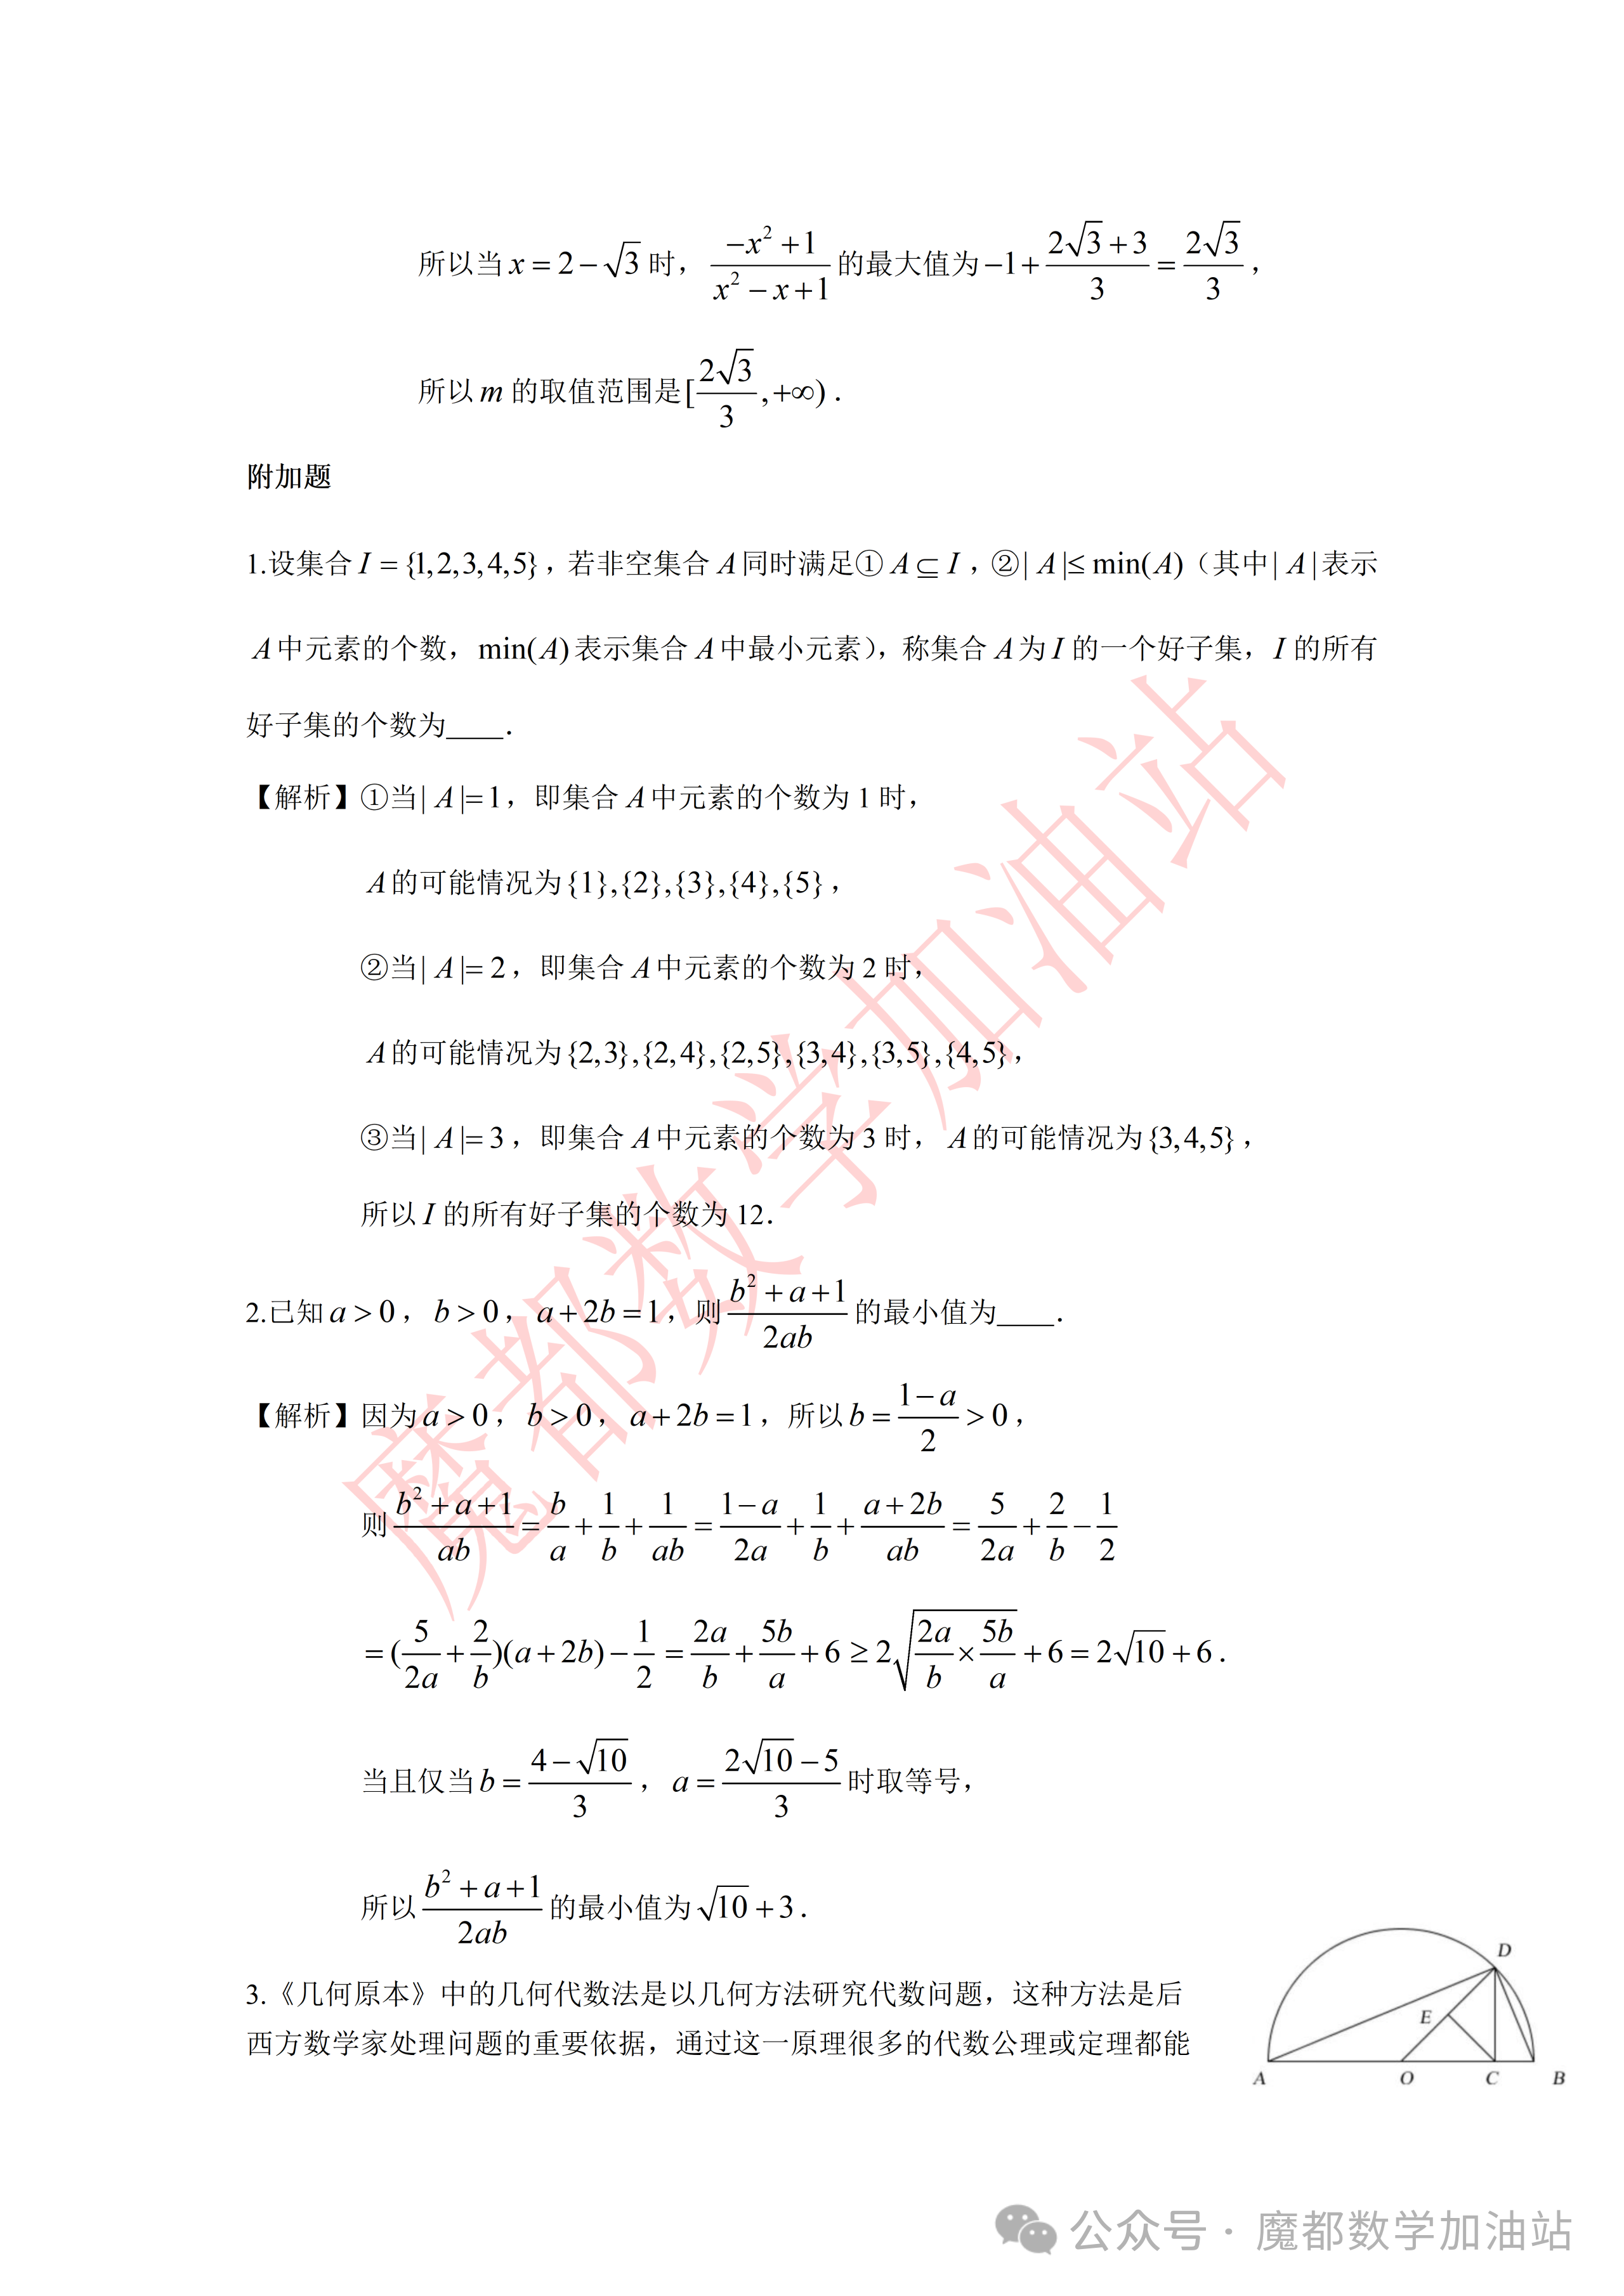
\includegraphics[width=.34\linewidth,trim=1960bp 310bp 90bp 3015bp,clip]{../原图/高一47_七宝中学_抱孩子练习9.26/08.png}
\end{center}

① $\dfrac{a+b}{2}\geqslant\sqrt{ab}$（$a>0$，$b>0$）；
② $a^2+b^2\geqslant2ab$（$a>0$，$b>0$）；
③ $\sqrt{ab}\geqslant\dfrac{2}{\dfrac1a+\dfrac1b}$（$a>0$，$b>0$）；
④ $\sqrt{\dfrac{a^2+b^2}{2}}\geqslant\dfrac{a+b}{2}$（$a>0$，$b>0$）.

\ifanswer
\solbegin
\step{因为 $AC+CB=a+b$，所以 $OD=\dfrac{AB}{2}=\dfrac{AC+CB}{2}=\dfrac{a+b}{2}$；}
\step{由射影定理得 $CD=\sqrt{AC\times CB}=\sqrt{ab}$，又因为 $OD\geqslant CD$，}
\step{所以 $\dfrac{a+b}{2}\geqslant\sqrt{ab}$，故①正确；}
\step{由射影定理得 $CD^2=DE\times OD$，所以 $DE=\dfrac{CD^2}{OD}=\dfrac{ab}{\dfrac{a+b}{2}}=\dfrac{2}{\dfrac1a+\dfrac1b}$，}
\step{又因为 $CD\geqslant DE$，所以 $\sqrt{ab}\geqslant\dfrac{2}{\dfrac1a+\dfrac1b}$，故③正确；}
\step{故该图形可以完成的所有无字证明为①③.}
\solend

\fi

% 注：原卷此处印作等式 $|x^2+a|+|x-a|=|x^2+x|$（在 $x>0$ 时与三角不等式下界等价），本稿曾改写成
% 不等式，现按原卷照录（原卷如此，照录未改）。
\item 若对任意 $x\in[2,3]$，均有 $|x^2+a|+|x-a|=|x^2+x|$，则实数 $a$ 的取值范围为 \blankline[4.4em].

\ifanswer
\solbegin
\step{因为 $|a|+|b|=|a+b|$ 当且仅当 $ab\geqslant0$ 时取等号，}
\step{所以 $(x^2+a)(x-a)\geqslant0$，即 $(a+x^2)(a-x)\leqslant0$，所以 $-x^2\leqslant a\leqslant x$ 恒成立，}
\step{因为 $x\in[2,3]$，所以 $-4\leqslant a\leqslant2$，所以实数 $a$ 的取值范围为 $[-4,2]$.}
\solend

\fi

\end{enumerate}

\end{document}
"
% 紧凑版：xelatex "\def\iscompact{1}% 高一47_七宝中学_抱孩子练习9.26.tex
%   —— 高一上数学“2026-2027 年七宝中学高一上抱孩子练习 9.26”（试卷版/答案版）
% 试卷版：xelatex 高一47_七宝中学_抱孩子练习9.26.tex
% 答案版：xelatex "\def\isanswer{1}% 高一47_七宝中学_抱孩子练习9.26.tex
%   —— 高一上数学“2026-2027 年七宝中学高一上抱孩子练习 9.26”（试卷版/答案版）
% 试卷版：xelatex 高一47_七宝中学_抱孩子练习9.26.tex
% 答案版：xelatex "\def\isanswer{1}% 高一47_七宝中学_抱孩子练习9.26.tex
%   —— 高一上数学“2026-2027 年七宝中学高一上抱孩子练习 9.26”（试卷版/答案版）
% 试卷版：xelatex 高一47_七宝中学_抱孩子练习9.26.tex
% 答案版：xelatex "\def\isanswer{1}\input{高一47_七宝中学_抱孩子练习9.26.tex}"
% 紧凑版：xelatex "\def\iscompact{1}\input{高一47_七宝中学_抱孩子练习9.26.tex}"
%
% 原始材料是微信公众号图文（公众号“魔都数学加油站”连载“27学年高一47”，署名“破晓”，
% 2026-10-02 17:56 发布，原文标题“27学年高一47——2026-2027年上海市七宝中学高一上抱孩子练习9.26”，
% 原文链接 https://mp.weixin.qq.com/s/mhkyDwjn7QFP_Z_NOcPkQA），正文为 9 张 PNG 页。
% 第 1—7、9 页分辨率为 4762×6735，第 8 页为 2560×3620；均按原图逐页核对。
% 原卷文字、选项、答案与解析均照录；粉色斜水印及灰色公众号页脚属水印/页脚，未录入。
%
% 卷首标题：原卷印作“2026-2027 年七宝中学高一上抱孩子练习 9.26”（公众号标题里的“上海市”
% 三字卷面标题行没有，本稿照卷面），年份区间按全稿惯例排 en dash，作业名保留原卷日期“9.26”。
% 原卷未印独立副标题；本稿按“知识模块”口径补出“集合与常用逻辑用语、不等式”。
%
% 与原卷的排版差异：
%   ① 原卷分“一、填空题”“二、选择题”“三、解答题”“附加题”四节；前三节题号为 3—16，
%      分别有 8 道填空、3 道选择、3 道解答；附加题另起 1—4 编号；
%   ② 原卷题下直接印答案/解析，本稿按全稿统一收进答案版；填空横线采用统一长度；
%   ③ 原卷未印副标题，本稿按“知识模块”口径补出（见卷首标题）；
%   ④ 全卷只有附加题第 3 题带图，直接从原卷第 8 页裁取。
%
% 原卷存疑（照录未改，见源码中该处上方注释）：
%   ① 第 9 题集合 C 的条件原文作“C={x|y=..., x 是整数}”，其中 y 未在集合描述中定义；
%      本稿照录原记号，未代换为 x。
%   ② 附加题第 3 题原文作“后西方数学家”，措辞存疑（疑漏“世”字）；本稿照录未改。
%
\documentclass[a4paper,11pt]{article}
\usepackage{common}

\begin{document}

\examtitlest[3]{2026--2027 年七宝中学高一上抱孩子练习 9.26}{集合与常用逻辑用语、不等式}

\bigsec{一、填空题}

\begin{enumerate}
\setcounter{enumi}{2}

\item 若不等式 $|x|<a$ 的一个充分条件为 $0<x<1$，则实数 $a$ 的取值范围是 \blankline[4.4em].

\ifanswer
\solbegin
\step{由 $|x|<a$ 得到 $-a<x<a$，}
\step{又不等式 $|x|<a$ 的一个充分条件为 $0<x<1$，所以 $a\geqslant1$.}
\solend

\fi

\item 已知命题“$\exists x\in\R$，使 $4x^2+(a-2)x+\dfrac14=0$”是假命题，则实数 $a$ 的取值范围是 \blankline[4.4em].

\ifanswer
\solbegin
% 注：原卷首句作“为真命题”（先按命题为真推出 $\Delta\geqslant0$，再由其为假得 $0<a<4$），原卷如此，照录未改。
\step{命题 $\exists x\in\R$，使 $4x^2+(a-2)x+\dfrac14=0$ 为真命题，}
\step{则 $\Delta=(a-2)^2-4\times4\times\dfrac14=a^2-4a\geqslant0$，解得 $a\leqslant0$ 或 $a\geqslant4$，}
\step{而命题“$\exists x\in\R$，使 $4x^2+(a-2)x+\dfrac14=0$”是假命题，则 $0<a<4$，}
\step{所以实数 $a$ 的取值范围是 $\{a\mid0<a<4\}$.}
\solend

\fi

\item 已知集合 $A=\{x\mid(a-1)x^2+3x-2=0\}$ 有且仅有两个子集，则实数 $a=$ \blankline[4.4em].

\ifanswer
\solbegin
\step{集合 $A=\{x\mid(a-1)x^2+3x-2=0\}$ 有且仅有两个不同的子集，}
\step{所以 $a-1=0$ 或 $\begin{cases}a-1\neq0\\\Delta=9+8(a-1)=0\end{cases}$，解得实数 $a=1$ 或 $a=-\dfrac18$.}
\solend

\fi

\item 已知函数 $y=x^2+bx+3$（其中 $b$ 是实数）中，$y$ 的取值范围是 $[0,+\infty)$，若关于 $x$ 的不等式 $x^2+bx+3<c$ 的解集为 $m-8<x<m$，则实数 $c$ 的值为 \blankline[4.4em].

\ifanswer
\solbegin
\step{因为 $y$ 的取值范围是 $[0,+\infty)$，所以 $\Delta=b^2-12=0$，解得 $b^2=12$，}
\step{因为不等式 $x^2+bx+3<c$ 的解集为 $m-8<x<m$，}
\step{令 $x^2+bx+3=c$，即 $x^2+bx+3-c=0$，方程的两根为 $x_1=m-8$，$x_2=m$，}
\step{所以 $|x_2-x_1|=\sqrt{(x_1+x_2)^2-4x_1x_2}=\sqrt{b^2-4(3-c)}=8$，即 $\sqrt{12-4(3-c)}=8$，}
\step{且判别式 $\Delta=b^2-4(3-c)=12-4(3-c)>0$，解得 $c=16$.}
\solend

\fi

\item 关于 $x$ 的不等式 $|x-1|+|x+1|\geqslant a$ 的解集为 $\R$，则实数 $a$ 的取值范围为 \blankline[4.4em].

\ifanswer
\solbegin
\step{因为 $|x-1|+|x+1|\geqslant|x-1-(x+1)|=2$，}
\step{若关于 $x$ 的不等式 $|x-1|+|x+1|\geqslant a$ 的解集为 $\R$，则实数 $a$ 的取值范围为 $a\leqslant2$.}
\solend

\fi

\item 已知 $m>0$，$xy>0$，当 $x+y=2$ 时，不等式 $\dfrac2x+\dfrac my\geqslant4$ 恒成立，则 $m$ 的取值范围是 \blankline[4.4em].

\ifanswer
\solbegin
\step{因为 $m>0$，$xy>0$，$x+y=2$，}
\step{所以 $\dfrac2x+\dfrac my=\dfrac12(x+y)\left(\dfrac2x+\dfrac my\right)
=\dfrac12\left(m+2+\dfrac{2y}{x}+\dfrac{mx}{y}\right)$}
\step{$\geqslant\dfrac12\left(m+2+2\sqrt{\dfrac{2y}{x}\cdot\dfrac{mx}{y}}\right)=\dfrac12\left(m+2+2\sqrt{2m}\right)$，}
\step{当且仅当 $\dfrac{2y}{x}=\dfrac{mx}{y}$，即 $y^2=\dfrac{mx^2}{2}$ 时取等号.}
\step{因为不等式 $\dfrac2x+\dfrac my\geqslant4$ 恒成立，所以 $\dfrac12(m+2+2\sqrt{2m})\geqslant4$，}
\step{整理得 $(\sqrt m+3\sqrt2)(\sqrt m-\sqrt2)\geqslant0$，解得 $\sqrt m\geqslant\sqrt2$，即 $m\geqslant2$，}
\step{所以 $m$ 的取值范围为 $[2,+\infty)$.}
\solend

\fi

\item 已知全集为 $\R$，集合 $D=\{x\mid x^2-ax+a^2-19=0\}$，
$B=\{y\mid y=-x^2+2x+2,\ y\text{ 是正整数}\}$，
% 注：本题集合 C 的条件原文作“C={x|y=..., x 是整数}”，其中 y 未在集合描述中定义；照录未改。
集合 $C=\left\{x\mathrel{\Big|}y=\sqrt{\dfrac{2-x}{x+1}},\ x\text{ 是整数}\right\}$，且集合 $D$ 满足 $D\cap B\neq\varnothing$，$\overline{D}\cup\overline{C}=\R$，则实数 $a$ 的值是 \blankline[4.4em].

\ifanswer
\solbegin
\step{集合 $B=\{y\mid y=-x^2+2x+2,\ y\text{ 是正整数}\}=\{1,2,3\}$，}
\step{集合 $C=\left\{x\mathrel{\Big|}y=\sqrt{\dfrac{2-x}{x+1}},\ x\text{ 是整数}\right\}=\{0,1,2\}$，}
\step{集合 $D=\{x\mid x^2-ax+a^2-19=0\}$ 且集合 $D$ 满足 $D\cap B\neq\varnothing$，$\overline{D}\cup\overline{C}=\R$，}
\step{所以 $3\in D$，解得 $a=5$ 或 $a=-2$，}
\step{经检验，$a=5$ 不符合 $\overline{D}\cup\overline{C}=\R$，舍去，$a=-2$ 满足题意，即 $a=-2$.}
\solend

\fi

% 注：本题解析中，$a=\pm2\sqrt2$ 时 $B$ 的二重根按 $-\dfrac a2$ 应为 $\mp\sqrt2$，原卷印作 $\mp2\sqrt2$、
% $-\dfrac{3\sqrt2}4$，$C(B)=3$ 的计算也随之按原卷保留（原卷如此，照录未改）。
\item 用 $C(A)$ 表示非空集合 $A$ 中的元素的个数，定义 $A*B=|C(A)-C(B)|$，已知集合 $A$ 有三个真子集，
$B=\{x\mid(ax^2+3x)(x^2+ax+2)=0,\ x\in\R\}$，若 $A*B=1$，设实数 $a$ 所有可能取值构成集合 $S$，则 $C(S)=$ \blankline[4.4em].

\ifanswer
\solbegin
\step{集合 $A$ 有三个真子集，则集合 $A$ 中有 $2$ 个元素，则 $C(A)=2$，}
\step{由 $A*B=1$，得 $C(B)=1$ 或 $3$，}
\step{即方程 $(ax^2+3x)\cdot(x^2+ax+2)=0$ 有一个根或 $3$ 个根；}
\step{若 $(ax^2+3x)\cdot(x^2+ax+2)=0$，则必有 $ax^2+3x=0$ 或 $x^2+ax+2=0$，}
\step{若 $ax^2+3x=0$，则 $x=0$ 或 $ax+3=0$，}
\step{当 $a=0$ 时，$B=\{0\}$，$C(B)=1$，符合题意；}
\step{当 $a\neq0$ 时，$ax^2+3x=0$ 对应的根为 $0$ 和 $-\dfrac3a$；}
\step{故①需 $x^2+ax+2=0$ 有两等根且根不为 $0$ 和 $-\dfrac3a$，}
\step{当 $\Delta=0$ 时，$a=\pm2\sqrt2$，}
\step{$a=2\sqrt2$，此时 $B=\left\{0,-2\sqrt2,-\dfrac{3\sqrt2}{4}\right\}$，$C(B)=3$，符合题意；}
\step{$a=-2\sqrt2$，此时 $B=\left\{0,2\sqrt2,\dfrac{3\sqrt2}{4}\right\}$，$C(B)=3$，符合题意；}
\step{②当 $-\dfrac3a$ 是 $x^2+ax+2=0$ 的根时，解得 $a=\pm3$；}
\step{$a=3$，此时 $B=\{0,-1,-2\}$，$C(B)=3$，符合题意；}
\step{$a=-3$，此时 $B=\{0,1,2\}$，$C(B)=3$，符合题意；}
\step{综上，$a$ 可取的值为 $0$、$\pm3$、$\pm2\sqrt2$，则 $C(S)=5$.}
\solend

\fi

\end{enumerate}

\bigsec{二、选择题}

\begin{enumerate}
\setcounter{enumi}{10}

\item 已知集合 $A=\left\{x\mathrel{\Big|}\dfrac1x<1\right\}$，$B=\{x\mid x^2-2x-3\leqslant0\}$，则 $A\cap B=$\mbox{（\quad）}

\keepwithprev
A. $\{x\mid1<x\leqslant3\}$\qquad B. $\{x\mid1\leqslant x\leqslant3\text{ 或 }-1\leqslant x<0\}$

C. $\{x\mid-1\leqslant x<0\}$\qquad D. $\{x\mid1<x\leqslant3\text{ 或 }-1\leqslant x<0\}$

\ans{$D$}

% 注：原卷本题只有题干＋选项（答案印在括号内），没有解析；此处照录原卷的"无解析"状态，不排解析。
\item 使 $x(y-2)=0$ 成立的一个充分条件是\mbox{（\quad）}

\keepwithprev
A. $x^2+(y-2)^2=0$\qquad B. $(x-2)^2+y^2=0$

C. $x^2+y^2=1$\qquad D. $x+y-2=0$

\ans{$A$}

\ifanswer
\solbegin
\step{对于 $A$：若 $x^2+(y-2)^2=0$，则 $x=0$ 且 $y=2$，此时 $x(y-2)=0$ 成立，}
\step{即充分性成立.}
\step{若 $x(y-2)=0$，则 $x=0$ 或 $y=2$，当 $x=0$，$y=3$ 时，$x^2+(y-2)^2=0$ 不成立，}
\step{即必要性不成立，}
\step{故 $x^2+(y-2)^2=0$ 是 $x(y-2)=0$ 成立的充分不必要条件；}
\step{对于 $B$：$(x-2)^2+y^2=0$，则 $x=2$ 且 $y=0$，此时 $x(y-2)=0$ 不成立，}
\step{即充分性不成立；}
\step{对于 $C$：$x^2+y^2=1$，此时 $x(y-2)=0$ 不一定成立，即充分性不成立；}
\step{对于 $D$：$x+y-2=0$，此时 $x(y-2)=0$ 不一定成立，即充分性不成立.}
\step{故选 $A$.}
\solend

\fi

\item 已知 $a$、$b$、$c\in\R$，若关于 $x$ 的不等式 $0\leqslant x+\dfrac ax+b\leqslant\dfrac cx-1$ 的解集为 $[x_1,x_2]\cup\{x_3\}$（$x_3>x_2>x_1>0$），则\mbox{（\quad）}

\keepwithprev
A. 不存在有序数组 $(a,b,c)$，使得 $x_2-x_1=1$

B. 存在唯一有序数组 $(a,b,c)$，使得 $x_2-x_1=1$

C. 有且只有两组有序数组 $(a,b,c)$，使得 $x_2-x_1=1$

D. 存在无穷多组有序数组 $(a,b,c)$，使得 $x_2-x_1=1$

\ans{$D$}

\ifanswer
\solbegin
\step{因为不等式 $0\leqslant x+\dfrac ax+b\leqslant\dfrac cx-1$ 的解集为 $[x_1,x_2]\cup\{x_3\}$（$x_3>x_2>x_1>0$），}
\step{所以 $0\leqslant x^2+bx+a\leqslant c-x$ 在 $[x_1,x_2]\cup\{x_3\}$ 上成立，}
\step{假设 $x_1=m$，$x_2=m+1$，$x_3=n$，}
\step{则 $c-n=0=n^2+bn+a$，由 $x_3$ 为一个独立的数得出，}
\step{所以 $n=c$，且 $m+1$ 与 $n$ 为方程 $x^2+bx+a=0$ 的两个根，}
\step{因为 $x_3>x_2>x_1>0$，所以 $-b=m+n+1=m+c+1$，$a=mn+n=mc+c$，}
\step{所以 $b=-m-c-1$，}
\step{且点 $(x_1,x_1^2+bx_1+a)$ 为 $y=x^2+bx+a$ 与 $y=c-x$ 的左交点，}
\step{所以 $m^2+bm+a=c-m$ 且 $b=-m-c-1$，$a=mc+c$，}
% 注：原卷此行的末句作“所以 $c-m=c-m$ 恒成立”（未写成 $x_2-x_1=1$），原卷如此，照录未改。
\step{故 $m^2+bm+a=m^2-m^2-mc-m+mc+c=c-m$，所以 $c-m=c-m$ 恒成立，}
\step{所以不论 $a$、$b$、$c$ 取何值，$x_2-x_1=1$ 恒成立，}
\step{即存在无穷多组有序数组 $(a,b,c)$，使得 $x_2-x_1=1$，}
\step{故选项 $A$、$B$、$C$ 错误，选项 $D$ 正确. 故选 $D$.}
\solend

\fi

\end{enumerate}

\bigsec{三、解答题}

\begin{enumerate}
\setcounter{enumi}{13}

\item 设正实数 $x$、$y$，满足 $2x+y=1$，求：

\begin{enumerate}[label=(\arabic*)]
\item $\sqrt{2x}+\sqrt y$ 的最大值；
\item $\dfrac2x+\dfrac1y$ 的最小值.
\end{enumerate}

\ifanswer
\solbegin
\stepm{(1)}{对于 $(\sqrt{2x}+\sqrt y)^2=2x+y+2\sqrt{2xy}\leqslant1+1=2$，}
\step{当且仅当 $\sqrt{2x}=\sqrt y$ 时取等号，故 $\sqrt{2x}+\sqrt y$ 的最大值为 $\sqrt2$；}
\stepm{(2)}{$\dfrac2x+\dfrac1y=\left(\dfrac2x+\dfrac1y\right)(2x+y)=5+\dfrac{2y}{x}+\dfrac{2x}{y}\geqslant5+4=9$，}
\step{当且仅当 $\dfrac{2y}{x}=\dfrac{2x}{y}$，即 $x=y=\dfrac13$ 时取等号，故 $\dfrac2x+\dfrac1y$ 的最小值为 $9$.}
\solend

\fi

\ansspace[6]

\item 设 $x_1$、$x_2$ 为关于 $x$ 的方程 $x^2-2(m+2)x+m^2-1=0$ 的两实数根.

\begin{enumerate}[label=(\arabic*)]
\item 若 $x_1$、$x_2$ 满足 $x_1^2+x_2^2=18$，试求 $m$ 的值；
\item 若 $x_1$、$x_2$ 均大于 $0$，求 $m$ 的取值范围.
\end{enumerate}

\ifanswer
\solbegin
\stepm{(1)}{由 $\Delta=4(m+2)^2-4(m^2-1)\geqslant0$，解得 $m\geqslant-\dfrac54$，}
\step{由韦达定理得 $x_1+x_2=2(m+2)$，$x_1x_2=m^2-1$，}
\step{又 $x_1^2+x_2^2=(x_1+x_2)^2-2x_1x_2=4(m+2)^2-2(m^2-1)=18$，}
\step{即 $m^2+8m=0$，解得 $m=0$ 或 $m=-8$（舍），故 $m$ 的值为 $0$；}
% 注：原卷此处作“由（2）得”（对照上一小问，所指应为（1）），原卷如此，照录未改。
\stepm{(2)}{由（2）得 $m\geqslant-\dfrac54$，}
\step{又 $x_1$、$x_2$ 均大于 $0$，则 $\begin{cases}2(m+2)>0\\m^2-1>0\end{cases}$，解得 $\begin{cases}m>-2\\m>1\text{或}m<-1\end{cases}$，}
\step{综上，实数 $m$ 的取值范围为 $\left[-\dfrac54,-1\right)\cup(1,+\infty)$.}
\solend

\fi

\ansspace[6]

\item 已知函数 $f(x)=(m+1)x^2-mx+m-1$（$m\in\R$）.

\begin{enumerate}[label=(\arabic*)]
\item 若不等式 $f(x)<0$ 的解集是空集，求 $m$ 的取值范围；
\item 当 $m>-2$ 时，解不等式 $f(x)\geqslant m$；
\item 若不等式 $f(x)\geqslant0$ 的解集为 $D$，若 $[-1,1]\subseteq D$，求 $m$ 的取值范围.
\end{enumerate}

\ifanswer
\solbegin
\stepm{(1)}{①当 $m+1=0$，即 $m=-1$ 时，$f(x)=x-2$，不合题意；}
\step{②当 $m+1\neq0$，即 $m\neq-1$ 时，$\begin{cases}m+1>0\\\Delta=m^2-4(m+1)(m-1)\leqslant0\end{cases}$，解得 $m\geqslant\dfrac{2\sqrt3}{3}$，}
\step{所以 $m$ 的取值范围是 $\left[\dfrac{2\sqrt3}{3},+\infty\right)$；}
\stepm{(2)}{因为 $f(x)\geqslant m$，所以 $(m+1)x^2-mx-1\geqslant0$，即 $[(m+1)x+1](x-1)\geqslant0$，}
\step{①当 $m+1=0$ 即 $m=-1$ 时，不等式的解集为 $[1,+\infty)$；}
\step{②当 $m+1>0$ 即 $m>-1$ 时，$\left(x+\dfrac1{m+1}\right)(x-1)\geqslant0$，}
\step{因为 $-\dfrac1{m+1}<0$，所以不等式的解集为 $\left(-\infty,-\dfrac1{m+1}\right]\cup[1,+\infty)$；}
\step{③当 $m+1<0$ 即 $-2<m<-1$ 时，$\left(x+\dfrac1{m+1}\right)(x-1)\leqslant0$，}
\step{因为 $-2<m<-1$，所以 $-1<m+1<0$，所以 $-\dfrac1{m+1}>1$，}
\step{所以不等式的解集为 $\left[1,-\dfrac1{m+1}\right]$；}
\stepm{(3)}{不等式 $f(x)\geqslant0$ 的解集为 $D$，若 $[-1,1]\subseteq D$，}
\step{即对任意的 $x\in[-1,1]$，不等式 $(m+1)x^2-mx+m-1\geqslant0$ 恒成立，}
\step{即 $m(x^2-x+1)\geqslant-x^2+1$ 恒成立，}
\step{因为 $x^2-x+1>0$ 恒成立，所以 $m\geqslant\dfrac{-x^2+1}{x^2-x+1}=-1+\dfrac{2-x}{x^2-x+1}$ 恒成立，}
\step{设 $t=2-x$，则 $t\in[1,3]$，$x=2-t$，}
\step{则 $\dfrac{2-x}{x^2-x+1}=\dfrac{t}{(2-t)^2-(2-t)+1}=\dfrac{t}{t^2-3t+3}=\dfrac1{t+\dfrac3t-3}$，}
\step{因为 $t+\dfrac3t\geqslant2\sqrt3$，当且仅当 $t=\sqrt3$ 时取等号，}
\step{所以 $\dfrac{2-x}{x^2-x+1}\leqslant\dfrac1{2\sqrt3-3}=\dfrac{2\sqrt3+3}{3}$，当且仅当 $x=2-\sqrt3$ 时取等号，}
\step{所以当 $x=2-\sqrt3$ 时，$\dfrac{-x^2+1}{x^2-x+1}$ 的最大值为 $-1+\dfrac{2\sqrt3+3}{3}=\dfrac{2\sqrt3}{3}$，}
\step{所以 $m$ 的取值范围是 $\left[\dfrac{2\sqrt3}{3},+\infty\right)$.}
\solend

\fi

\ansspace[8]

\end{enumerate}

\bigsec{附加题}

\begin{enumerate}

\item 设集合 $I=\{1,2,3,4,5\}$，若非空集合 $A$ 同时满足① $A\subseteq I$，② $|A|\leqslant\min(A)$（其中 $|A|$ 表示集合 $A$ 中元素的个数，$\min(A)$ 表示集合 $A$ 中最小元素），称集合 $A$ 为 $I$ 的一个好子集，$I$ 所有好子集的个数为 \blankline[4.4em].

\ifanswer
\solbegin
\step{①当 $|A|=1$，即集合 $A$ 中元素的个数为 $1$ 时，}
\step{$A$ 的可能情况为 $\{1\}$、$\{2\}$、$\{3\}$、$\{4\}$、$\{5\}$，}
\step{②当 $|A|=2$，即集合 $A$ 中元素的个数为 $2$ 时，}
\step{$A$ 的可能情况为 $\{2,3\}$、$\{2,4\}$、$\{2,5\}$、$\{3,4\}$、$\{3,5\}$、$\{4,5\}$，}
\step{③当 $|A|=3$，即集合 $A$ 中元素的个数为 $3$ 时，$A$ 的可能情况为 $\{3,4,5\}$，}
\step{所以 $I$ 的所有好子集的个数为 $12$.}
\solend

\fi

\item 已知 $a>0$，$b>0$，$a+2b=1$，则 $\dfrac{b^2+a+1}{2ab}$ 的最小值为 \blankline[4.4em].

\ifanswer
\solbegin
\step{因为 $a>0$，$b>0$，$a+2b=1$，所以 $b=\dfrac{1-a}{2}>0$，}
\step{则 $\dfrac{b^2+a+1}{ab}=\dfrac ba+\dfrac1b+\dfrac1{ab}=\dfrac{1-a}{2a}+\dfrac1b+\dfrac{a+2b}{ab}=\dfrac5{2a}+\dfrac2b-\dfrac12$}
\step{$=\left(\dfrac5{2a}+\dfrac2b\right)(a+2b)-\dfrac12=\dfrac{2a}{b}+\dfrac{5b}{a}+6\geqslant2\sqrt{\dfrac{2a}{b}\times\dfrac{5b}{a}}+6=2\sqrt{10}+6$.}
\step{当且仅当 $b=\dfrac{4-\sqrt{10}}{3}$，$a=\dfrac{2\sqrt{10}-5}{3}$ 时取等号，}
\step{所以 $\dfrac{b^2+a+1}{2ab}$ 的最小值为 $\sqrt{10}+3$.}
\solend

\fi

% 注：本题原文作“后西方数学家”，措辞存疑（疑漏“世”字）；照录未改，见文件头“原卷存疑”②。
% 又原文作"很多的代数公理或定理都能够通过图形实现证明"（"公理"疑为"公式"笔误）、
% "连结 OD,AD,BD"，均原卷如此，照录未改。
\item 《几何原本》中的几何代数法是以几何方法研究代数问题，这种方法是后西方数学家处理问题的重要依据，通过这一原理很多的代数公理或定理都能够通过图形实现证明，也称之为无字证明，现有图形如图所示，$C$ 为线段 $AB$ 上的点，且 $AC=a$，$BC=b$，$O$ 为 $AB$ 的中点，以 $AB$ 为直径作半圆，过点 $C$ 作 $AB$ 的垂线交半圆于 $D$，连结 $OD,AD,BD$，过点 $C$ 作 $OD$ 的垂线，垂足为 $E$，若不添加辅助线，则该图形可以完成的所有无字证明为 \blankline[4.4em]（填写序号）.

\begin{center}
% 插图直接裁自原卷第 8 页，未重绘；用 trim/clip 保留原图与标注。
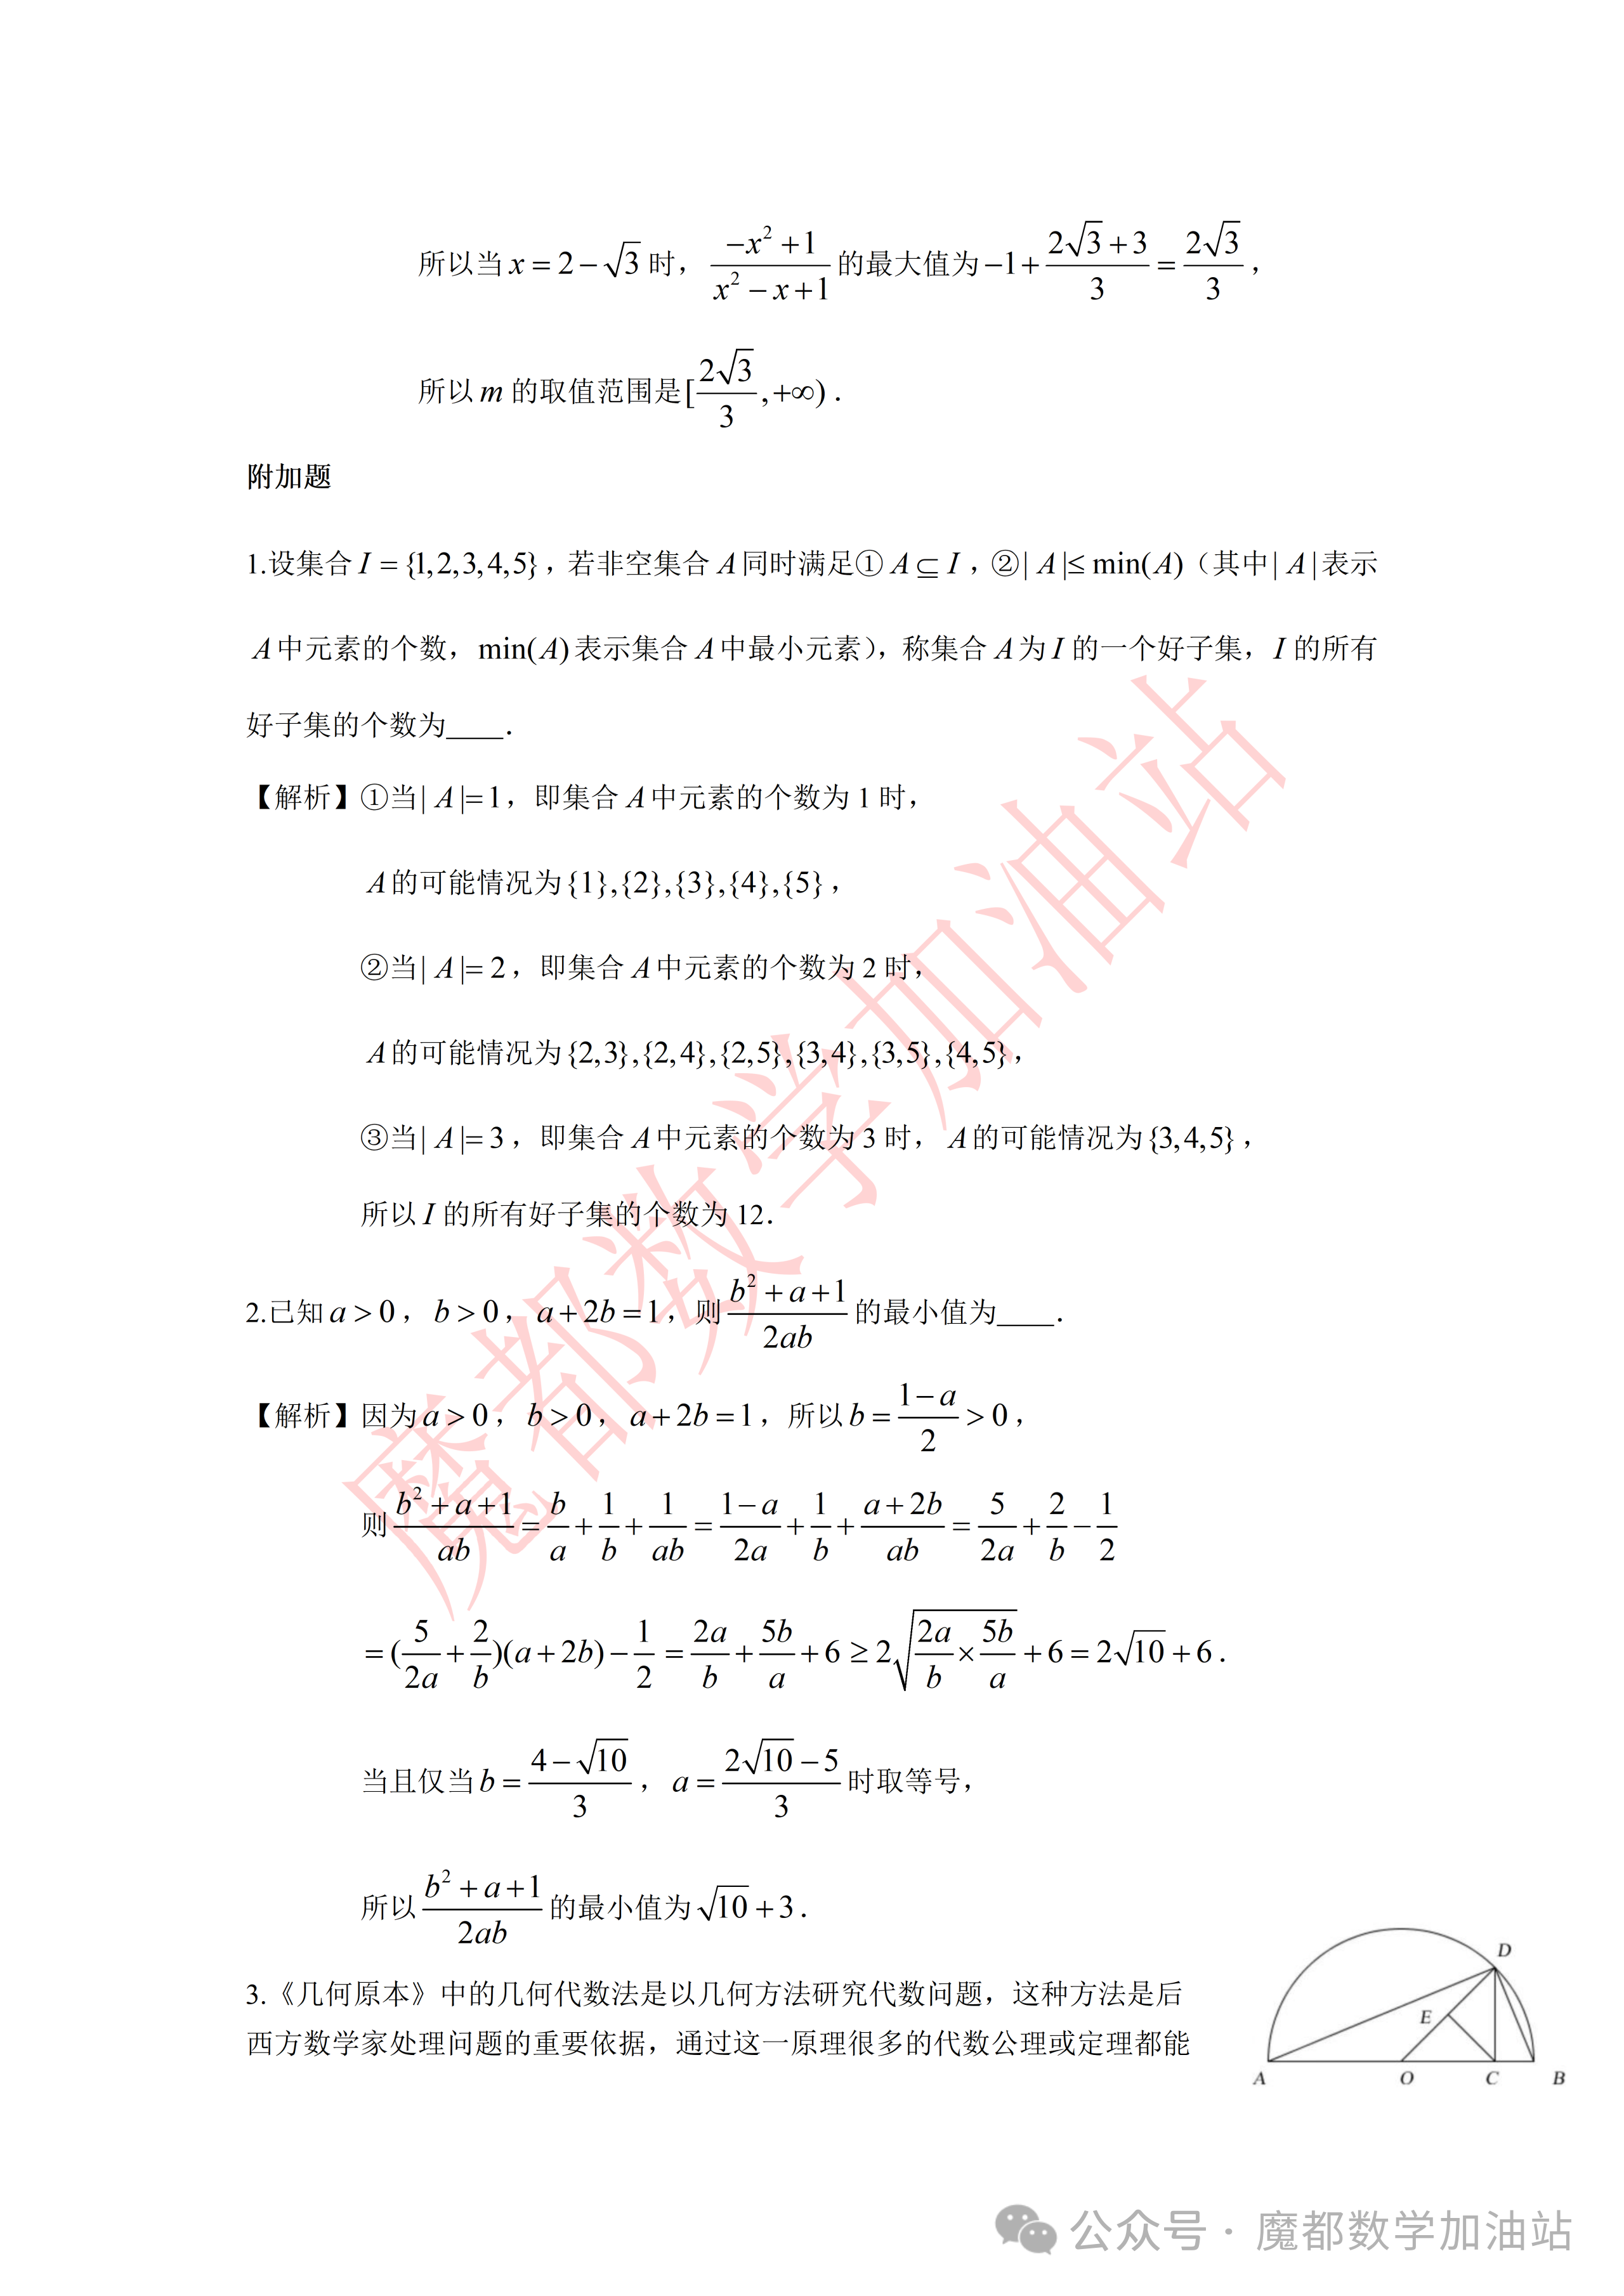
\includegraphics[width=.34\linewidth,trim=1960bp 310bp 90bp 3015bp,clip]{../原图/高一47_七宝中学_抱孩子练习9.26/08.png}
\end{center}

① $\dfrac{a+b}{2}\geqslant\sqrt{ab}$（$a>0$，$b>0$）；
② $a^2+b^2\geqslant2ab$（$a>0$，$b>0$）；
③ $\sqrt{ab}\geqslant\dfrac{2}{\dfrac1a+\dfrac1b}$（$a>0$，$b>0$）；
④ $\sqrt{\dfrac{a^2+b^2}{2}}\geqslant\dfrac{a+b}{2}$（$a>0$，$b>0$）.

\ifanswer
\solbegin
\step{因为 $AC+CB=a+b$，所以 $OD=\dfrac{AB}{2}=\dfrac{AC+CB}{2}=\dfrac{a+b}{2}$；}
\step{由射影定理得 $CD=\sqrt{AC\times CB}=\sqrt{ab}$，又因为 $OD\geqslant CD$，}
\step{所以 $\dfrac{a+b}{2}\geqslant\sqrt{ab}$，故①正确；}
\step{由射影定理得 $CD^2=DE\times OD$，所以 $DE=\dfrac{CD^2}{OD}=\dfrac{ab}{\dfrac{a+b}{2}}=\dfrac{2}{\dfrac1a+\dfrac1b}$，}
\step{又因为 $CD\geqslant DE$，所以 $\sqrt{ab}\geqslant\dfrac{2}{\dfrac1a+\dfrac1b}$，故③正确；}
\step{故该图形可以完成的所有无字证明为①③.}
\solend

\fi

% 注：原卷此处印作等式 $|x^2+a|+|x-a|=|x^2+x|$（在 $x>0$ 时与三角不等式下界等价），本稿曾改写成
% 不等式，现按原卷照录（原卷如此，照录未改）。
\item 若对任意 $x\in[2,3]$，均有 $|x^2+a|+|x-a|=|x^2+x|$，则实数 $a$ 的取值范围为 \blankline[4.4em].

\ifanswer
\solbegin
\step{因为 $|a|+|b|=|a+b|$ 当且仅当 $ab\geqslant0$ 时取等号，}
\step{所以 $(x^2+a)(x-a)\geqslant0$，即 $(a+x^2)(a-x)\leqslant0$，所以 $-x^2\leqslant a\leqslant x$ 恒成立，}
\step{因为 $x\in[2,3]$，所以 $-4\leqslant a\leqslant2$，所以实数 $a$ 的取值范围为 $[-4,2]$.}
\solend

\fi

\end{enumerate}

\end{document}
"
% 紧凑版：xelatex "\def\iscompact{1}% 高一47_七宝中学_抱孩子练习9.26.tex
%   —— 高一上数学“2026-2027 年七宝中学高一上抱孩子练习 9.26”（试卷版/答案版）
% 试卷版：xelatex 高一47_七宝中学_抱孩子练习9.26.tex
% 答案版：xelatex "\def\isanswer{1}\input{高一47_七宝中学_抱孩子练习9.26.tex}"
% 紧凑版：xelatex "\def\iscompact{1}\input{高一47_七宝中学_抱孩子练习9.26.tex}"
%
% 原始材料是微信公众号图文（公众号“魔都数学加油站”连载“27学年高一47”，署名“破晓”，
% 2026-10-02 17:56 发布，原文标题“27学年高一47——2026-2027年上海市七宝中学高一上抱孩子练习9.26”，
% 原文链接 https://mp.weixin.qq.com/s/mhkyDwjn7QFP_Z_NOcPkQA），正文为 9 张 PNG 页。
% 第 1—7、9 页分辨率为 4762×6735，第 8 页为 2560×3620；均按原图逐页核对。
% 原卷文字、选项、答案与解析均照录；粉色斜水印及灰色公众号页脚属水印/页脚，未录入。
%
% 卷首标题：原卷印作“2026-2027 年七宝中学高一上抱孩子练习 9.26”（公众号标题里的“上海市”
% 三字卷面标题行没有，本稿照卷面），年份区间按全稿惯例排 en dash，作业名保留原卷日期“9.26”。
% 原卷未印独立副标题；本稿按“知识模块”口径补出“集合与常用逻辑用语、不等式”。
%
% 与原卷的排版差异：
%   ① 原卷分“一、填空题”“二、选择题”“三、解答题”“附加题”四节；前三节题号为 3—16，
%      分别有 8 道填空、3 道选择、3 道解答；附加题另起 1—4 编号；
%   ② 原卷题下直接印答案/解析，本稿按全稿统一收进答案版；填空横线采用统一长度；
%   ③ 原卷未印副标题，本稿按“知识模块”口径补出（见卷首标题）；
%   ④ 全卷只有附加题第 3 题带图，直接从原卷第 8 页裁取。
%
% 原卷存疑（照录未改，见源码中该处上方注释）：
%   ① 第 9 题集合 C 的条件原文作“C={x|y=..., x 是整数}”，其中 y 未在集合描述中定义；
%      本稿照录原记号，未代换为 x。
%   ② 附加题第 3 题原文作“后西方数学家”，措辞存疑（疑漏“世”字）；本稿照录未改。
%
\documentclass[a4paper,11pt]{article}
\usepackage{common}

\begin{document}

\examtitlest[3]{2026--2027 年七宝中学高一上抱孩子练习 9.26}{集合与常用逻辑用语、不等式}

\bigsec{一、填空题}

\begin{enumerate}
\setcounter{enumi}{2}

\item 若不等式 $|x|<a$ 的一个充分条件为 $0<x<1$，则实数 $a$ 的取值范围是 \blankline[4.4em].

\ifanswer
\solbegin
\step{由 $|x|<a$ 得到 $-a<x<a$，}
\step{又不等式 $|x|<a$ 的一个充分条件为 $0<x<1$，所以 $a\geqslant1$.}
\solend

\fi

\item 已知命题“$\exists x\in\R$，使 $4x^2+(a-2)x+\dfrac14=0$”是假命题，则实数 $a$ 的取值范围是 \blankline[4.4em].

\ifanswer
\solbegin
% 注：原卷首句作“为真命题”（先按命题为真推出 $\Delta\geqslant0$，再由其为假得 $0<a<4$），原卷如此，照录未改。
\step{命题 $\exists x\in\R$，使 $4x^2+(a-2)x+\dfrac14=0$ 为真命题，}
\step{则 $\Delta=(a-2)^2-4\times4\times\dfrac14=a^2-4a\geqslant0$，解得 $a\leqslant0$ 或 $a\geqslant4$，}
\step{而命题“$\exists x\in\R$，使 $4x^2+(a-2)x+\dfrac14=0$”是假命题，则 $0<a<4$，}
\step{所以实数 $a$ 的取值范围是 $\{a\mid0<a<4\}$.}
\solend

\fi

\item 已知集合 $A=\{x\mid(a-1)x^2+3x-2=0\}$ 有且仅有两个子集，则实数 $a=$ \blankline[4.4em].

\ifanswer
\solbegin
\step{集合 $A=\{x\mid(a-1)x^2+3x-2=0\}$ 有且仅有两个不同的子集，}
\step{所以 $a-1=0$ 或 $\begin{cases}a-1\neq0\\\Delta=9+8(a-1)=0\end{cases}$，解得实数 $a=1$ 或 $a=-\dfrac18$.}
\solend

\fi

\item 已知函数 $y=x^2+bx+3$（其中 $b$ 是实数）中，$y$ 的取值范围是 $[0,+\infty)$，若关于 $x$ 的不等式 $x^2+bx+3<c$ 的解集为 $m-8<x<m$，则实数 $c$ 的值为 \blankline[4.4em].

\ifanswer
\solbegin
\step{因为 $y$ 的取值范围是 $[0,+\infty)$，所以 $\Delta=b^2-12=0$，解得 $b^2=12$，}
\step{因为不等式 $x^2+bx+3<c$ 的解集为 $m-8<x<m$，}
\step{令 $x^2+bx+3=c$，即 $x^2+bx+3-c=0$，方程的两根为 $x_1=m-8$，$x_2=m$，}
\step{所以 $|x_2-x_1|=\sqrt{(x_1+x_2)^2-4x_1x_2}=\sqrt{b^2-4(3-c)}=8$，即 $\sqrt{12-4(3-c)}=8$，}
\step{且判别式 $\Delta=b^2-4(3-c)=12-4(3-c)>0$，解得 $c=16$.}
\solend

\fi

\item 关于 $x$ 的不等式 $|x-1|+|x+1|\geqslant a$ 的解集为 $\R$，则实数 $a$ 的取值范围为 \blankline[4.4em].

\ifanswer
\solbegin
\step{因为 $|x-1|+|x+1|\geqslant|x-1-(x+1)|=2$，}
\step{若关于 $x$ 的不等式 $|x-1|+|x+1|\geqslant a$ 的解集为 $\R$，则实数 $a$ 的取值范围为 $a\leqslant2$.}
\solend

\fi

\item 已知 $m>0$，$xy>0$，当 $x+y=2$ 时，不等式 $\dfrac2x+\dfrac my\geqslant4$ 恒成立，则 $m$ 的取值范围是 \blankline[4.4em].

\ifanswer
\solbegin
\step{因为 $m>0$，$xy>0$，$x+y=2$，}
\step{所以 $\dfrac2x+\dfrac my=\dfrac12(x+y)\left(\dfrac2x+\dfrac my\right)
=\dfrac12\left(m+2+\dfrac{2y}{x}+\dfrac{mx}{y}\right)$}
\step{$\geqslant\dfrac12\left(m+2+2\sqrt{\dfrac{2y}{x}\cdot\dfrac{mx}{y}}\right)=\dfrac12\left(m+2+2\sqrt{2m}\right)$，}
\step{当且仅当 $\dfrac{2y}{x}=\dfrac{mx}{y}$，即 $y^2=\dfrac{mx^2}{2}$ 时取等号.}
\step{因为不等式 $\dfrac2x+\dfrac my\geqslant4$ 恒成立，所以 $\dfrac12(m+2+2\sqrt{2m})\geqslant4$，}
\step{整理得 $(\sqrt m+3\sqrt2)(\sqrt m-\sqrt2)\geqslant0$，解得 $\sqrt m\geqslant\sqrt2$，即 $m\geqslant2$，}
\step{所以 $m$ 的取值范围为 $[2,+\infty)$.}
\solend

\fi

\item 已知全集为 $\R$，集合 $D=\{x\mid x^2-ax+a^2-19=0\}$，
$B=\{y\mid y=-x^2+2x+2,\ y\text{ 是正整数}\}$，
% 注：本题集合 C 的条件原文作“C={x|y=..., x 是整数}”，其中 y 未在集合描述中定义；照录未改。
集合 $C=\left\{x\mathrel{\Big|}y=\sqrt{\dfrac{2-x}{x+1}},\ x\text{ 是整数}\right\}$，且集合 $D$ 满足 $D\cap B\neq\varnothing$，$\overline{D}\cup\overline{C}=\R$，则实数 $a$ 的值是 \blankline[4.4em].

\ifanswer
\solbegin
\step{集合 $B=\{y\mid y=-x^2+2x+2,\ y\text{ 是正整数}\}=\{1,2,3\}$，}
\step{集合 $C=\left\{x\mathrel{\Big|}y=\sqrt{\dfrac{2-x}{x+1}},\ x\text{ 是整数}\right\}=\{0,1,2\}$，}
\step{集合 $D=\{x\mid x^2-ax+a^2-19=0\}$ 且集合 $D$ 满足 $D\cap B\neq\varnothing$，$\overline{D}\cup\overline{C}=\R$，}
\step{所以 $3\in D$，解得 $a=5$ 或 $a=-2$，}
\step{经检验，$a=5$ 不符合 $\overline{D}\cup\overline{C}=\R$，舍去，$a=-2$ 满足题意，即 $a=-2$.}
\solend

\fi

% 注：本题解析中，$a=\pm2\sqrt2$ 时 $B$ 的二重根按 $-\dfrac a2$ 应为 $\mp\sqrt2$，原卷印作 $\mp2\sqrt2$、
% $-\dfrac{3\sqrt2}4$，$C(B)=3$ 的计算也随之按原卷保留（原卷如此，照录未改）。
\item 用 $C(A)$ 表示非空集合 $A$ 中的元素的个数，定义 $A*B=|C(A)-C(B)|$，已知集合 $A$ 有三个真子集，
$B=\{x\mid(ax^2+3x)(x^2+ax+2)=0,\ x\in\R\}$，若 $A*B=1$，设实数 $a$ 所有可能取值构成集合 $S$，则 $C(S)=$ \blankline[4.4em].

\ifanswer
\solbegin
\step{集合 $A$ 有三个真子集，则集合 $A$ 中有 $2$ 个元素，则 $C(A)=2$，}
\step{由 $A*B=1$，得 $C(B)=1$ 或 $3$，}
\step{即方程 $(ax^2+3x)\cdot(x^2+ax+2)=0$ 有一个根或 $3$ 个根；}
\step{若 $(ax^2+3x)\cdot(x^2+ax+2)=0$，则必有 $ax^2+3x=0$ 或 $x^2+ax+2=0$，}
\step{若 $ax^2+3x=0$，则 $x=0$ 或 $ax+3=0$，}
\step{当 $a=0$ 时，$B=\{0\}$，$C(B)=1$，符合题意；}
\step{当 $a\neq0$ 时，$ax^2+3x=0$ 对应的根为 $0$ 和 $-\dfrac3a$；}
\step{故①需 $x^2+ax+2=0$ 有两等根且根不为 $0$ 和 $-\dfrac3a$，}
\step{当 $\Delta=0$ 时，$a=\pm2\sqrt2$，}
\step{$a=2\sqrt2$，此时 $B=\left\{0,-2\sqrt2,-\dfrac{3\sqrt2}{4}\right\}$，$C(B)=3$，符合题意；}
\step{$a=-2\sqrt2$，此时 $B=\left\{0,2\sqrt2,\dfrac{3\sqrt2}{4}\right\}$，$C(B)=3$，符合题意；}
\step{②当 $-\dfrac3a$ 是 $x^2+ax+2=0$ 的根时，解得 $a=\pm3$；}
\step{$a=3$，此时 $B=\{0,-1,-2\}$，$C(B)=3$，符合题意；}
\step{$a=-3$，此时 $B=\{0,1,2\}$，$C(B)=3$，符合题意；}
\step{综上，$a$ 可取的值为 $0$、$\pm3$、$\pm2\sqrt2$，则 $C(S)=5$.}
\solend

\fi

\end{enumerate}

\bigsec{二、选择题}

\begin{enumerate}
\setcounter{enumi}{10}

\item 已知集合 $A=\left\{x\mathrel{\Big|}\dfrac1x<1\right\}$，$B=\{x\mid x^2-2x-3\leqslant0\}$，则 $A\cap B=$\mbox{（\quad）}

\keepwithprev
A. $\{x\mid1<x\leqslant3\}$\qquad B. $\{x\mid1\leqslant x\leqslant3\text{ 或 }-1\leqslant x<0\}$

C. $\{x\mid-1\leqslant x<0\}$\qquad D. $\{x\mid1<x\leqslant3\text{ 或 }-1\leqslant x<0\}$

\ans{$D$}

% 注：原卷本题只有题干＋选项（答案印在括号内），没有解析；此处照录原卷的"无解析"状态，不排解析。
\item 使 $x(y-2)=0$ 成立的一个充分条件是\mbox{（\quad）}

\keepwithprev
A. $x^2+(y-2)^2=0$\qquad B. $(x-2)^2+y^2=0$

C. $x^2+y^2=1$\qquad D. $x+y-2=0$

\ans{$A$}

\ifanswer
\solbegin
\step{对于 $A$：若 $x^2+(y-2)^2=0$，则 $x=0$ 且 $y=2$，此时 $x(y-2)=0$ 成立，}
\step{即充分性成立.}
\step{若 $x(y-2)=0$，则 $x=0$ 或 $y=2$，当 $x=0$，$y=3$ 时，$x^2+(y-2)^2=0$ 不成立，}
\step{即必要性不成立，}
\step{故 $x^2+(y-2)^2=0$ 是 $x(y-2)=0$ 成立的充分不必要条件；}
\step{对于 $B$：$(x-2)^2+y^2=0$，则 $x=2$ 且 $y=0$，此时 $x(y-2)=0$ 不成立，}
\step{即充分性不成立；}
\step{对于 $C$：$x^2+y^2=1$，此时 $x(y-2)=0$ 不一定成立，即充分性不成立；}
\step{对于 $D$：$x+y-2=0$，此时 $x(y-2)=0$ 不一定成立，即充分性不成立.}
\step{故选 $A$.}
\solend

\fi

\item 已知 $a$、$b$、$c\in\R$，若关于 $x$ 的不等式 $0\leqslant x+\dfrac ax+b\leqslant\dfrac cx-1$ 的解集为 $[x_1,x_2]\cup\{x_3\}$（$x_3>x_2>x_1>0$），则\mbox{（\quad）}

\keepwithprev
A. 不存在有序数组 $(a,b,c)$，使得 $x_2-x_1=1$

B. 存在唯一有序数组 $(a,b,c)$，使得 $x_2-x_1=1$

C. 有且只有两组有序数组 $(a,b,c)$，使得 $x_2-x_1=1$

D. 存在无穷多组有序数组 $(a,b,c)$，使得 $x_2-x_1=1$

\ans{$D$}

\ifanswer
\solbegin
\step{因为不等式 $0\leqslant x+\dfrac ax+b\leqslant\dfrac cx-1$ 的解集为 $[x_1,x_2]\cup\{x_3\}$（$x_3>x_2>x_1>0$），}
\step{所以 $0\leqslant x^2+bx+a\leqslant c-x$ 在 $[x_1,x_2]\cup\{x_3\}$ 上成立，}
\step{假设 $x_1=m$，$x_2=m+1$，$x_3=n$，}
\step{则 $c-n=0=n^2+bn+a$，由 $x_3$ 为一个独立的数得出，}
\step{所以 $n=c$，且 $m+1$ 与 $n$ 为方程 $x^2+bx+a=0$ 的两个根，}
\step{因为 $x_3>x_2>x_1>0$，所以 $-b=m+n+1=m+c+1$，$a=mn+n=mc+c$，}
\step{所以 $b=-m-c-1$，}
\step{且点 $(x_1,x_1^2+bx_1+a)$ 为 $y=x^2+bx+a$ 与 $y=c-x$ 的左交点，}
\step{所以 $m^2+bm+a=c-m$ 且 $b=-m-c-1$，$a=mc+c$，}
% 注：原卷此行的末句作“所以 $c-m=c-m$ 恒成立”（未写成 $x_2-x_1=1$），原卷如此，照录未改。
\step{故 $m^2+bm+a=m^2-m^2-mc-m+mc+c=c-m$，所以 $c-m=c-m$ 恒成立，}
\step{所以不论 $a$、$b$、$c$ 取何值，$x_2-x_1=1$ 恒成立，}
\step{即存在无穷多组有序数组 $(a,b,c)$，使得 $x_2-x_1=1$，}
\step{故选项 $A$、$B$、$C$ 错误，选项 $D$ 正确. 故选 $D$.}
\solend

\fi

\end{enumerate}

\bigsec{三、解答题}

\begin{enumerate}
\setcounter{enumi}{13}

\item 设正实数 $x$、$y$，满足 $2x+y=1$，求：

\begin{enumerate}[label=(\arabic*)]
\item $\sqrt{2x}+\sqrt y$ 的最大值；
\item $\dfrac2x+\dfrac1y$ 的最小值.
\end{enumerate}

\ifanswer
\solbegin
\stepm{(1)}{对于 $(\sqrt{2x}+\sqrt y)^2=2x+y+2\sqrt{2xy}\leqslant1+1=2$，}
\step{当且仅当 $\sqrt{2x}=\sqrt y$ 时取等号，故 $\sqrt{2x}+\sqrt y$ 的最大值为 $\sqrt2$；}
\stepm{(2)}{$\dfrac2x+\dfrac1y=\left(\dfrac2x+\dfrac1y\right)(2x+y)=5+\dfrac{2y}{x}+\dfrac{2x}{y}\geqslant5+4=9$，}
\step{当且仅当 $\dfrac{2y}{x}=\dfrac{2x}{y}$，即 $x=y=\dfrac13$ 时取等号，故 $\dfrac2x+\dfrac1y$ 的最小值为 $9$.}
\solend

\fi

\ansspace[6]

\item 设 $x_1$、$x_2$ 为关于 $x$ 的方程 $x^2-2(m+2)x+m^2-1=0$ 的两实数根.

\begin{enumerate}[label=(\arabic*)]
\item 若 $x_1$、$x_2$ 满足 $x_1^2+x_2^2=18$，试求 $m$ 的值；
\item 若 $x_1$、$x_2$ 均大于 $0$，求 $m$ 的取值范围.
\end{enumerate}

\ifanswer
\solbegin
\stepm{(1)}{由 $\Delta=4(m+2)^2-4(m^2-1)\geqslant0$，解得 $m\geqslant-\dfrac54$，}
\step{由韦达定理得 $x_1+x_2=2(m+2)$，$x_1x_2=m^2-1$，}
\step{又 $x_1^2+x_2^2=(x_1+x_2)^2-2x_1x_2=4(m+2)^2-2(m^2-1)=18$，}
\step{即 $m^2+8m=0$，解得 $m=0$ 或 $m=-8$（舍），故 $m$ 的值为 $0$；}
% 注：原卷此处作“由（2）得”（对照上一小问，所指应为（1）），原卷如此，照录未改。
\stepm{(2)}{由（2）得 $m\geqslant-\dfrac54$，}
\step{又 $x_1$、$x_2$ 均大于 $0$，则 $\begin{cases}2(m+2)>0\\m^2-1>0\end{cases}$，解得 $\begin{cases}m>-2\\m>1\text{或}m<-1\end{cases}$，}
\step{综上，实数 $m$ 的取值范围为 $\left[-\dfrac54,-1\right)\cup(1,+\infty)$.}
\solend

\fi

\ansspace[6]

\item 已知函数 $f(x)=(m+1)x^2-mx+m-1$（$m\in\R$）.

\begin{enumerate}[label=(\arabic*)]
\item 若不等式 $f(x)<0$ 的解集是空集，求 $m$ 的取值范围；
\item 当 $m>-2$ 时，解不等式 $f(x)\geqslant m$；
\item 若不等式 $f(x)\geqslant0$ 的解集为 $D$，若 $[-1,1]\subseteq D$，求 $m$ 的取值范围.
\end{enumerate}

\ifanswer
\solbegin
\stepm{(1)}{①当 $m+1=0$，即 $m=-1$ 时，$f(x)=x-2$，不合题意；}
\step{②当 $m+1\neq0$，即 $m\neq-1$ 时，$\begin{cases}m+1>0\\\Delta=m^2-4(m+1)(m-1)\leqslant0\end{cases}$，解得 $m\geqslant\dfrac{2\sqrt3}{3}$，}
\step{所以 $m$ 的取值范围是 $\left[\dfrac{2\sqrt3}{3},+\infty\right)$；}
\stepm{(2)}{因为 $f(x)\geqslant m$，所以 $(m+1)x^2-mx-1\geqslant0$，即 $[(m+1)x+1](x-1)\geqslant0$，}
\step{①当 $m+1=0$ 即 $m=-1$ 时，不等式的解集为 $[1,+\infty)$；}
\step{②当 $m+1>0$ 即 $m>-1$ 时，$\left(x+\dfrac1{m+1}\right)(x-1)\geqslant0$，}
\step{因为 $-\dfrac1{m+1}<0$，所以不等式的解集为 $\left(-\infty,-\dfrac1{m+1}\right]\cup[1,+\infty)$；}
\step{③当 $m+1<0$ 即 $-2<m<-1$ 时，$\left(x+\dfrac1{m+1}\right)(x-1)\leqslant0$，}
\step{因为 $-2<m<-1$，所以 $-1<m+1<0$，所以 $-\dfrac1{m+1}>1$，}
\step{所以不等式的解集为 $\left[1,-\dfrac1{m+1}\right]$；}
\stepm{(3)}{不等式 $f(x)\geqslant0$ 的解集为 $D$，若 $[-1,1]\subseteq D$，}
\step{即对任意的 $x\in[-1,1]$，不等式 $(m+1)x^2-mx+m-1\geqslant0$ 恒成立，}
\step{即 $m(x^2-x+1)\geqslant-x^2+1$ 恒成立，}
\step{因为 $x^2-x+1>0$ 恒成立，所以 $m\geqslant\dfrac{-x^2+1}{x^2-x+1}=-1+\dfrac{2-x}{x^2-x+1}$ 恒成立，}
\step{设 $t=2-x$，则 $t\in[1,3]$，$x=2-t$，}
\step{则 $\dfrac{2-x}{x^2-x+1}=\dfrac{t}{(2-t)^2-(2-t)+1}=\dfrac{t}{t^2-3t+3}=\dfrac1{t+\dfrac3t-3}$，}
\step{因为 $t+\dfrac3t\geqslant2\sqrt3$，当且仅当 $t=\sqrt3$ 时取等号，}
\step{所以 $\dfrac{2-x}{x^2-x+1}\leqslant\dfrac1{2\sqrt3-3}=\dfrac{2\sqrt3+3}{3}$，当且仅当 $x=2-\sqrt3$ 时取等号，}
\step{所以当 $x=2-\sqrt3$ 时，$\dfrac{-x^2+1}{x^2-x+1}$ 的最大值为 $-1+\dfrac{2\sqrt3+3}{3}=\dfrac{2\sqrt3}{3}$，}
\step{所以 $m$ 的取值范围是 $\left[\dfrac{2\sqrt3}{3},+\infty\right)$.}
\solend

\fi

\ansspace[8]

\end{enumerate}

\bigsec{附加题}

\begin{enumerate}

\item 设集合 $I=\{1,2,3,4,5\}$，若非空集合 $A$ 同时满足① $A\subseteq I$，② $|A|\leqslant\min(A)$（其中 $|A|$ 表示集合 $A$ 中元素的个数，$\min(A)$ 表示集合 $A$ 中最小元素），称集合 $A$ 为 $I$ 的一个好子集，$I$ 所有好子集的个数为 \blankline[4.4em].

\ifanswer
\solbegin
\step{①当 $|A|=1$，即集合 $A$ 中元素的个数为 $1$ 时，}
\step{$A$ 的可能情况为 $\{1\}$、$\{2\}$、$\{3\}$、$\{4\}$、$\{5\}$，}
\step{②当 $|A|=2$，即集合 $A$ 中元素的个数为 $2$ 时，}
\step{$A$ 的可能情况为 $\{2,3\}$、$\{2,4\}$、$\{2,5\}$、$\{3,4\}$、$\{3,5\}$、$\{4,5\}$，}
\step{③当 $|A|=3$，即集合 $A$ 中元素的个数为 $3$ 时，$A$ 的可能情况为 $\{3,4,5\}$，}
\step{所以 $I$ 的所有好子集的个数为 $12$.}
\solend

\fi

\item 已知 $a>0$，$b>0$，$a+2b=1$，则 $\dfrac{b^2+a+1}{2ab}$ 的最小值为 \blankline[4.4em].

\ifanswer
\solbegin
\step{因为 $a>0$，$b>0$，$a+2b=1$，所以 $b=\dfrac{1-a}{2}>0$，}
\step{则 $\dfrac{b^2+a+1}{ab}=\dfrac ba+\dfrac1b+\dfrac1{ab}=\dfrac{1-a}{2a}+\dfrac1b+\dfrac{a+2b}{ab}=\dfrac5{2a}+\dfrac2b-\dfrac12$}
\step{$=\left(\dfrac5{2a}+\dfrac2b\right)(a+2b)-\dfrac12=\dfrac{2a}{b}+\dfrac{5b}{a}+6\geqslant2\sqrt{\dfrac{2a}{b}\times\dfrac{5b}{a}}+6=2\sqrt{10}+6$.}
\step{当且仅当 $b=\dfrac{4-\sqrt{10}}{3}$，$a=\dfrac{2\sqrt{10}-5}{3}$ 时取等号，}
\step{所以 $\dfrac{b^2+a+1}{2ab}$ 的最小值为 $\sqrt{10}+3$.}
\solend

\fi

% 注：本题原文作“后西方数学家”，措辞存疑（疑漏“世”字）；照录未改，见文件头“原卷存疑”②。
% 又原文作"很多的代数公理或定理都能够通过图形实现证明"（"公理"疑为"公式"笔误）、
% "连结 OD,AD,BD"，均原卷如此，照录未改。
\item 《几何原本》中的几何代数法是以几何方法研究代数问题，这种方法是后西方数学家处理问题的重要依据，通过这一原理很多的代数公理或定理都能够通过图形实现证明，也称之为无字证明，现有图形如图所示，$C$ 为线段 $AB$ 上的点，且 $AC=a$，$BC=b$，$O$ 为 $AB$ 的中点，以 $AB$ 为直径作半圆，过点 $C$ 作 $AB$ 的垂线交半圆于 $D$，连结 $OD,AD,BD$，过点 $C$ 作 $OD$ 的垂线，垂足为 $E$，若不添加辅助线，则该图形可以完成的所有无字证明为 \blankline[4.4em]（填写序号）.

\begin{center}
% 插图直接裁自原卷第 8 页，未重绘；用 trim/clip 保留原图与标注。
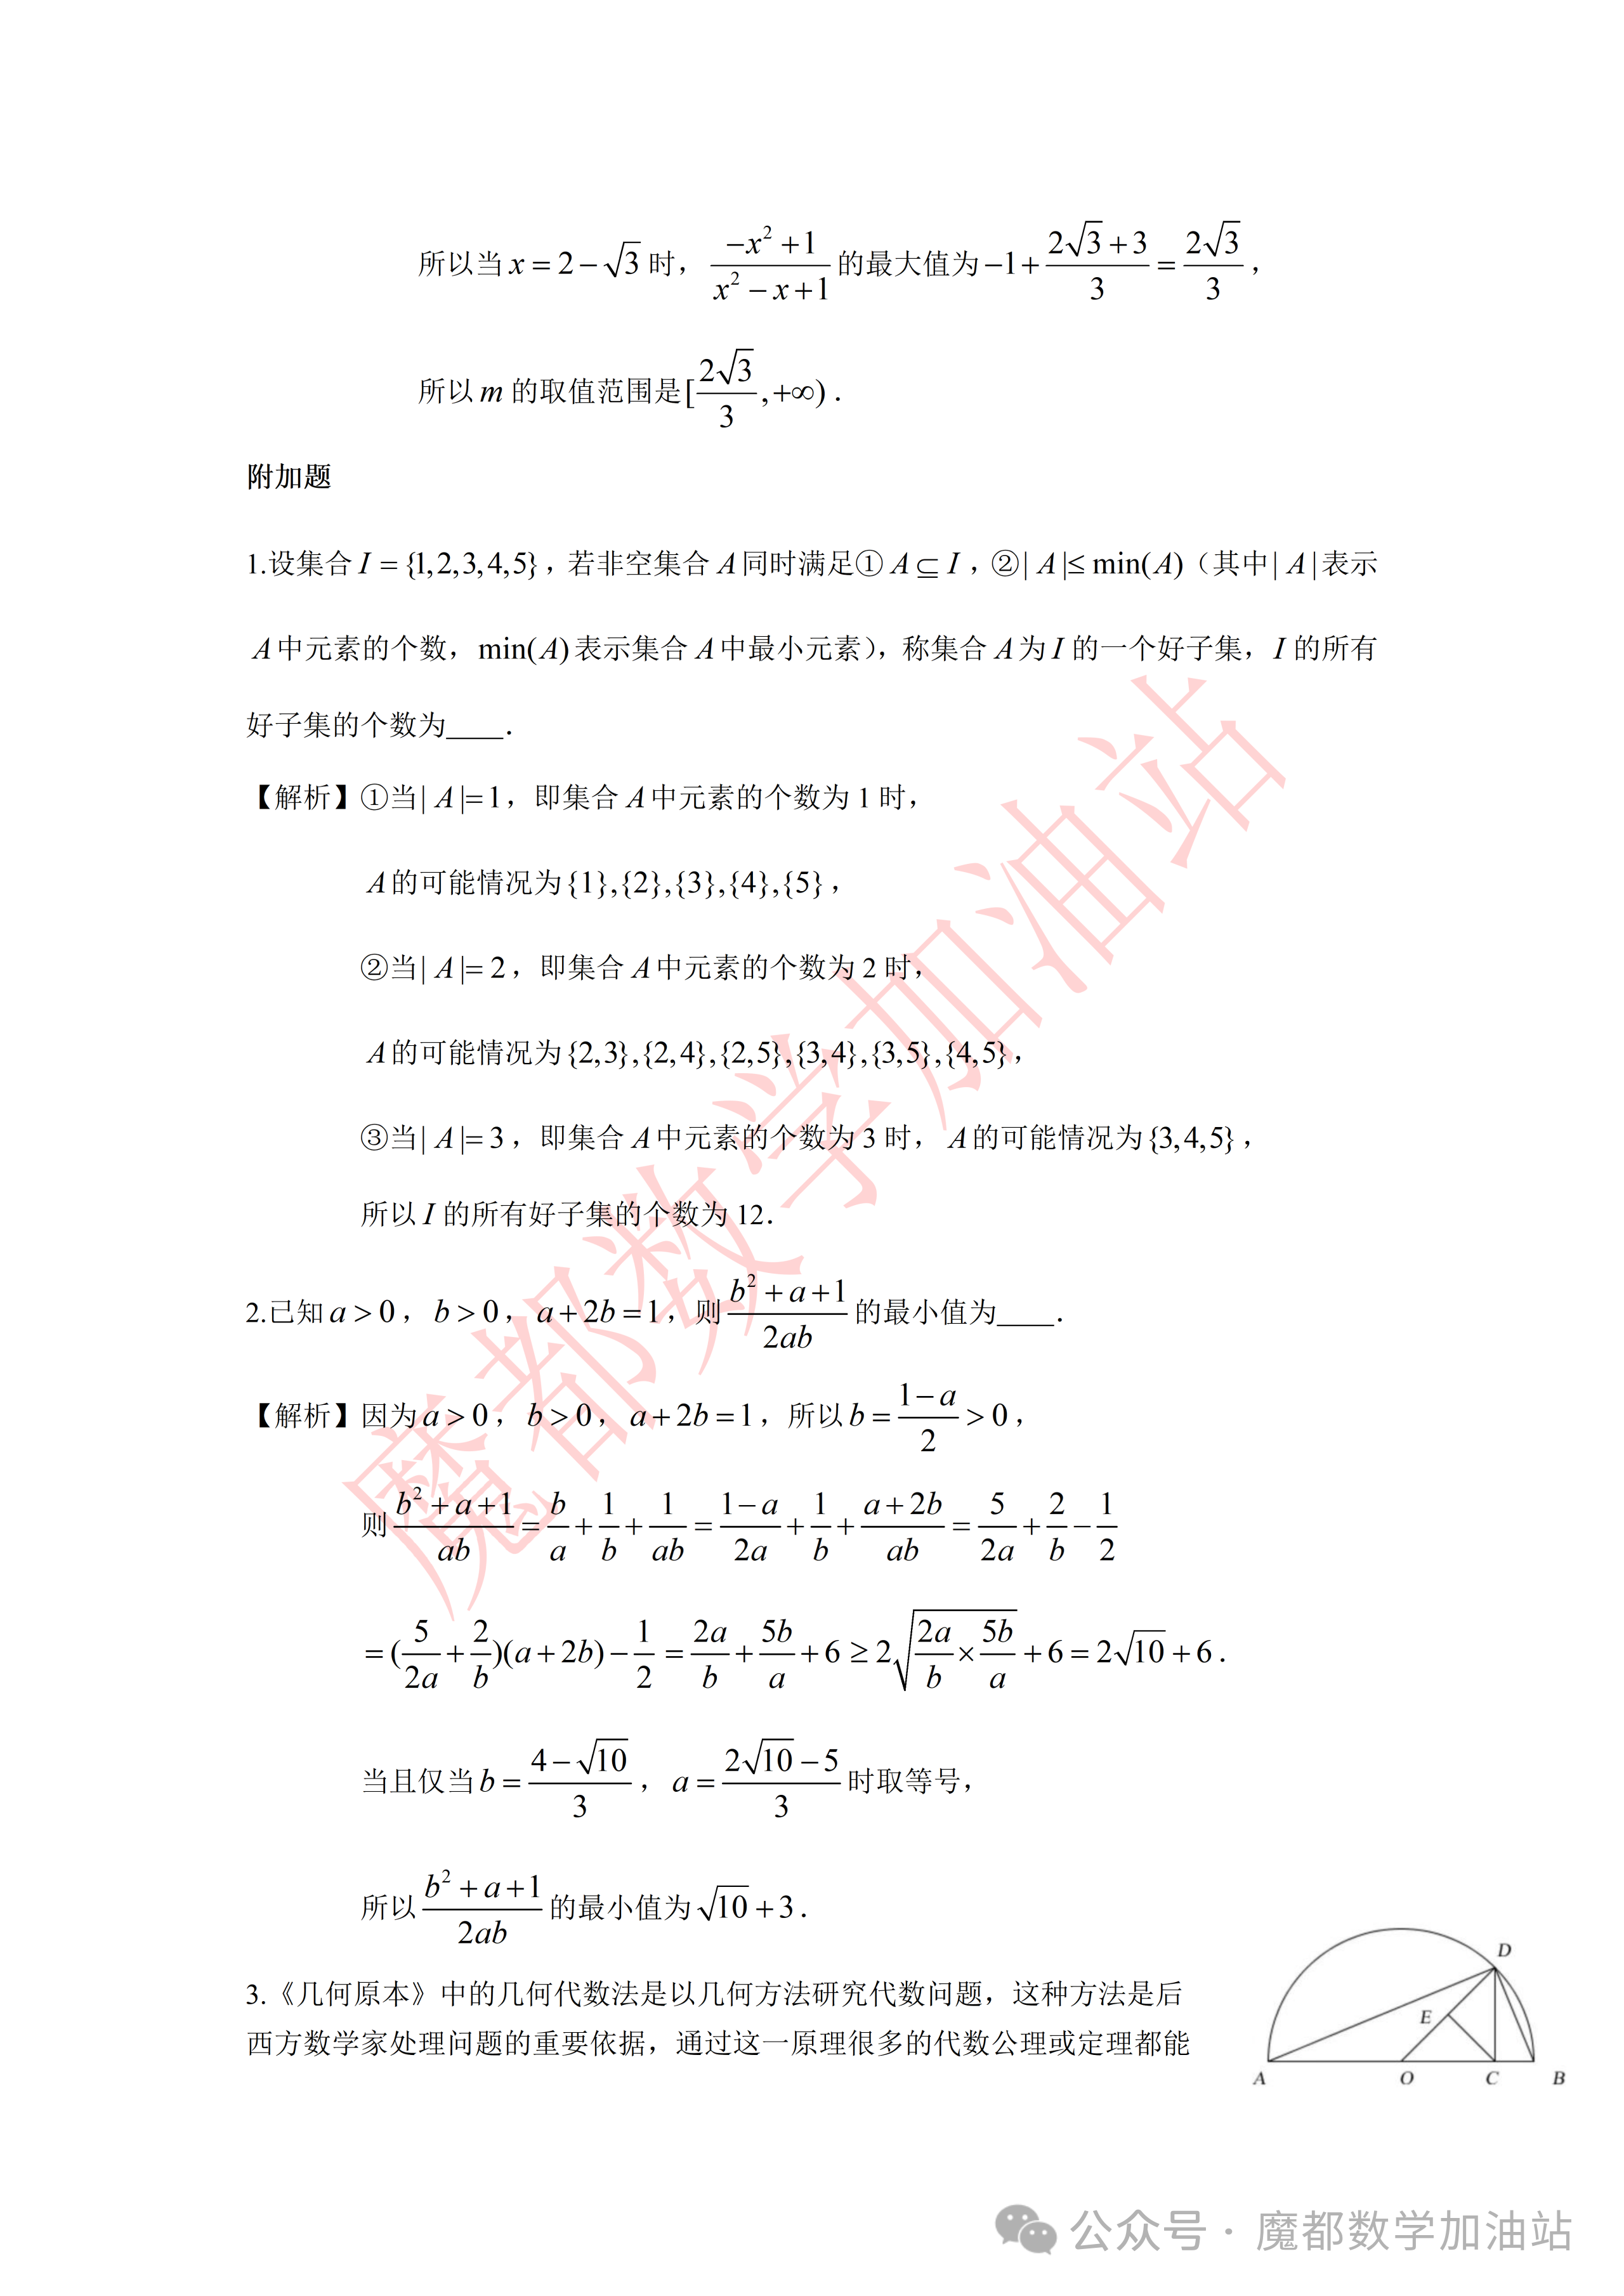
\includegraphics[width=.34\linewidth,trim=1960bp 310bp 90bp 3015bp,clip]{../原图/高一47_七宝中学_抱孩子练习9.26/08.png}
\end{center}

① $\dfrac{a+b}{2}\geqslant\sqrt{ab}$（$a>0$，$b>0$）；
② $a^2+b^2\geqslant2ab$（$a>0$，$b>0$）；
③ $\sqrt{ab}\geqslant\dfrac{2}{\dfrac1a+\dfrac1b}$（$a>0$，$b>0$）；
④ $\sqrt{\dfrac{a^2+b^2}{2}}\geqslant\dfrac{a+b}{2}$（$a>0$，$b>0$）.

\ifanswer
\solbegin
\step{因为 $AC+CB=a+b$，所以 $OD=\dfrac{AB}{2}=\dfrac{AC+CB}{2}=\dfrac{a+b}{2}$；}
\step{由射影定理得 $CD=\sqrt{AC\times CB}=\sqrt{ab}$，又因为 $OD\geqslant CD$，}
\step{所以 $\dfrac{a+b}{2}\geqslant\sqrt{ab}$，故①正确；}
\step{由射影定理得 $CD^2=DE\times OD$，所以 $DE=\dfrac{CD^2}{OD}=\dfrac{ab}{\dfrac{a+b}{2}}=\dfrac{2}{\dfrac1a+\dfrac1b}$，}
\step{又因为 $CD\geqslant DE$，所以 $\sqrt{ab}\geqslant\dfrac{2}{\dfrac1a+\dfrac1b}$，故③正确；}
\step{故该图形可以完成的所有无字证明为①③.}
\solend

\fi

% 注：原卷此处印作等式 $|x^2+a|+|x-a|=|x^2+x|$（在 $x>0$ 时与三角不等式下界等价），本稿曾改写成
% 不等式，现按原卷照录（原卷如此，照录未改）。
\item 若对任意 $x\in[2,3]$，均有 $|x^2+a|+|x-a|=|x^2+x|$，则实数 $a$ 的取值范围为 \blankline[4.4em].

\ifanswer
\solbegin
\step{因为 $|a|+|b|=|a+b|$ 当且仅当 $ab\geqslant0$ 时取等号，}
\step{所以 $(x^2+a)(x-a)\geqslant0$，即 $(a+x^2)(a-x)\leqslant0$，所以 $-x^2\leqslant a\leqslant x$ 恒成立，}
\step{因为 $x\in[2,3]$，所以 $-4\leqslant a\leqslant2$，所以实数 $a$ 的取值范围为 $[-4,2]$.}
\solend

\fi

\end{enumerate}

\end{document}
"
%
% 原始材料是微信公众号图文（公众号“魔都数学加油站”连载“27学年高一47”，署名“破晓”，
% 2026-10-02 17:56 发布，原文标题“27学年高一47——2026-2027年上海市七宝中学高一上抱孩子练习9.26”，
% 原文链接 https://mp.weixin.qq.com/s/mhkyDwjn7QFP_Z_NOcPkQA），正文为 9 张 PNG 页。
% 第 1—7、9 页分辨率为 4762×6735，第 8 页为 2560×3620；均按原图逐页核对。
% 原卷文字、选项、答案与解析均照录；粉色斜水印及灰色公众号页脚属水印/页脚，未录入。
%
% 卷首标题：原卷印作“2026-2027 年七宝中学高一上抱孩子练习 9.26”（公众号标题里的“上海市”
% 三字卷面标题行没有，本稿照卷面），年份区间按全稿惯例排 en dash，作业名保留原卷日期“9.26”。
% 原卷未印独立副标题；本稿按“知识模块”口径补出“集合与常用逻辑用语、不等式”。
%
% 与原卷的排版差异：
%   ① 原卷分“一、填空题”“二、选择题”“三、解答题”“附加题”四节；前三节题号为 3—16，
%      分别有 8 道填空、3 道选择、3 道解答；附加题另起 1—4 编号；
%   ② 原卷题下直接印答案/解析，本稿按全稿统一收进答案版；填空横线采用统一长度；
%   ③ 原卷未印副标题，本稿按“知识模块”口径补出（见卷首标题）；
%   ④ 全卷只有附加题第 3 题带图，直接从原卷第 8 页裁取。
%
% 原卷存疑（照录未改，见源码中该处上方注释）：
%   ① 第 9 题集合 C 的条件原文作“C={x|y=..., x 是整数}”，其中 y 未在集合描述中定义；
%      本稿照录原记号，未代换为 x。
%   ② 附加题第 3 题原文作“后西方数学家”，措辞存疑（疑漏“世”字）；本稿照录未改。
%
\documentclass[a4paper,11pt]{article}
\usepackage{common}

\begin{document}

\examtitlest[3]{2026--2027 年七宝中学高一上抱孩子练习 9.26}{集合与常用逻辑用语、不等式}

\bigsec{一、填空题}

\begin{enumerate}
\setcounter{enumi}{2}

\item 若不等式 $|x|<a$ 的一个充分条件为 $0<x<1$，则实数 $a$ 的取值范围是 \blankline[4.4em].

\ifanswer
\solbegin
\step{由 $|x|<a$ 得到 $-a<x<a$，}
\step{又不等式 $|x|<a$ 的一个充分条件为 $0<x<1$，所以 $a\geqslant1$.}
\solend

\fi

\item 已知命题“$\exists x\in\R$，使 $4x^2+(a-2)x+\dfrac14=0$”是假命题，则实数 $a$ 的取值范围是 \blankline[4.4em].

\ifanswer
\solbegin
% 注：原卷首句作“为真命题”（先按命题为真推出 $\Delta\geqslant0$，再由其为假得 $0<a<4$），原卷如此，照录未改。
\step{命题 $\exists x\in\R$，使 $4x^2+(a-2)x+\dfrac14=0$ 为真命题，}
\step{则 $\Delta=(a-2)^2-4\times4\times\dfrac14=a^2-4a\geqslant0$，解得 $a\leqslant0$ 或 $a\geqslant4$，}
\step{而命题“$\exists x\in\R$，使 $4x^2+(a-2)x+\dfrac14=0$”是假命题，则 $0<a<4$，}
\step{所以实数 $a$ 的取值范围是 $\{a\mid0<a<4\}$.}
\solend

\fi

\item 已知集合 $A=\{x\mid(a-1)x^2+3x-2=0\}$ 有且仅有两个子集，则实数 $a=$ \blankline[4.4em].

\ifanswer
\solbegin
\step{集合 $A=\{x\mid(a-1)x^2+3x-2=0\}$ 有且仅有两个不同的子集，}
\step{所以 $a-1=0$ 或 $\begin{cases}a-1\neq0\\\Delta=9+8(a-1)=0\end{cases}$，解得实数 $a=1$ 或 $a=-\dfrac18$.}
\solend

\fi

\item 已知函数 $y=x^2+bx+3$（其中 $b$ 是实数）中，$y$ 的取值范围是 $[0,+\infty)$，若关于 $x$ 的不等式 $x^2+bx+3<c$ 的解集为 $m-8<x<m$，则实数 $c$ 的值为 \blankline[4.4em].

\ifanswer
\solbegin
\step{因为 $y$ 的取值范围是 $[0,+\infty)$，所以 $\Delta=b^2-12=0$，解得 $b^2=12$，}
\step{因为不等式 $x^2+bx+3<c$ 的解集为 $m-8<x<m$，}
\step{令 $x^2+bx+3=c$，即 $x^2+bx+3-c=0$，方程的两根为 $x_1=m-8$，$x_2=m$，}
\step{所以 $|x_2-x_1|=\sqrt{(x_1+x_2)^2-4x_1x_2}=\sqrt{b^2-4(3-c)}=8$，即 $\sqrt{12-4(3-c)}=8$，}
\step{且判别式 $\Delta=b^2-4(3-c)=12-4(3-c)>0$，解得 $c=16$.}
\solend

\fi

\item 关于 $x$ 的不等式 $|x-1|+|x+1|\geqslant a$ 的解集为 $\R$，则实数 $a$ 的取值范围为 \blankline[4.4em].

\ifanswer
\solbegin
\step{因为 $|x-1|+|x+1|\geqslant|x-1-(x+1)|=2$，}
\step{若关于 $x$ 的不等式 $|x-1|+|x+1|\geqslant a$ 的解集为 $\R$，则实数 $a$ 的取值范围为 $a\leqslant2$.}
\solend

\fi

\item 已知 $m>0$，$xy>0$，当 $x+y=2$ 时，不等式 $\dfrac2x+\dfrac my\geqslant4$ 恒成立，则 $m$ 的取值范围是 \blankline[4.4em].

\ifanswer
\solbegin
\step{因为 $m>0$，$xy>0$，$x+y=2$，}
\step{所以 $\dfrac2x+\dfrac my=\dfrac12(x+y)\left(\dfrac2x+\dfrac my\right)
=\dfrac12\left(m+2+\dfrac{2y}{x}+\dfrac{mx}{y}\right)$}
\step{$\geqslant\dfrac12\left(m+2+2\sqrt{\dfrac{2y}{x}\cdot\dfrac{mx}{y}}\right)=\dfrac12\left(m+2+2\sqrt{2m}\right)$，}
\step{当且仅当 $\dfrac{2y}{x}=\dfrac{mx}{y}$，即 $y^2=\dfrac{mx^2}{2}$ 时取等号.}
\step{因为不等式 $\dfrac2x+\dfrac my\geqslant4$ 恒成立，所以 $\dfrac12(m+2+2\sqrt{2m})\geqslant4$，}
\step{整理得 $(\sqrt m+3\sqrt2)(\sqrt m-\sqrt2)\geqslant0$，解得 $\sqrt m\geqslant\sqrt2$，即 $m\geqslant2$，}
\step{所以 $m$ 的取值范围为 $[2,+\infty)$.}
\solend

\fi

\item 已知全集为 $\R$，集合 $D=\{x\mid x^2-ax+a^2-19=0\}$，
$B=\{y\mid y=-x^2+2x+2,\ y\text{ 是正整数}\}$，
% 注：本题集合 C 的条件原文作“C={x|y=..., x 是整数}”，其中 y 未在集合描述中定义；照录未改。
集合 $C=\left\{x\mathrel{\Big|}y=\sqrt{\dfrac{2-x}{x+1}},\ x\text{ 是整数}\right\}$，且集合 $D$ 满足 $D\cap B\neq\varnothing$，$\overline{D}\cup\overline{C}=\R$，则实数 $a$ 的值是 \blankline[4.4em].

\ifanswer
\solbegin
\step{集合 $B=\{y\mid y=-x^2+2x+2,\ y\text{ 是正整数}\}=\{1,2,3\}$，}
\step{集合 $C=\left\{x\mathrel{\Big|}y=\sqrt{\dfrac{2-x}{x+1}},\ x\text{ 是整数}\right\}=\{0,1,2\}$，}
\step{集合 $D=\{x\mid x^2-ax+a^2-19=0\}$ 且集合 $D$ 满足 $D\cap B\neq\varnothing$，$\overline{D}\cup\overline{C}=\R$，}
\step{所以 $3\in D$，解得 $a=5$ 或 $a=-2$，}
\step{经检验，$a=5$ 不符合 $\overline{D}\cup\overline{C}=\R$，舍去，$a=-2$ 满足题意，即 $a=-2$.}
\solend

\fi

% 注：本题解析中，$a=\pm2\sqrt2$ 时 $B$ 的二重根按 $-\dfrac a2$ 应为 $\mp\sqrt2$，原卷印作 $\mp2\sqrt2$、
% $-\dfrac{3\sqrt2}4$，$C(B)=3$ 的计算也随之按原卷保留（原卷如此，照录未改）。
\item 用 $C(A)$ 表示非空集合 $A$ 中的元素的个数，定义 $A*B=|C(A)-C(B)|$，已知集合 $A$ 有三个真子集，
$B=\{x\mid(ax^2+3x)(x^2+ax+2)=0,\ x\in\R\}$，若 $A*B=1$，设实数 $a$ 所有可能取值构成集合 $S$，则 $C(S)=$ \blankline[4.4em].

\ifanswer
\solbegin
\step{集合 $A$ 有三个真子集，则集合 $A$ 中有 $2$ 个元素，则 $C(A)=2$，}
\step{由 $A*B=1$，得 $C(B)=1$ 或 $3$，}
\step{即方程 $(ax^2+3x)\cdot(x^2+ax+2)=0$ 有一个根或 $3$ 个根；}
\step{若 $(ax^2+3x)\cdot(x^2+ax+2)=0$，则必有 $ax^2+3x=0$ 或 $x^2+ax+2=0$，}
\step{若 $ax^2+3x=0$，则 $x=0$ 或 $ax+3=0$，}
\step{当 $a=0$ 时，$B=\{0\}$，$C(B)=1$，符合题意；}
\step{当 $a\neq0$ 时，$ax^2+3x=0$ 对应的根为 $0$ 和 $-\dfrac3a$；}
\step{故①需 $x^2+ax+2=0$ 有两等根且根不为 $0$ 和 $-\dfrac3a$，}
\step{当 $\Delta=0$ 时，$a=\pm2\sqrt2$，}
\step{$a=2\sqrt2$，此时 $B=\left\{0,-2\sqrt2,-\dfrac{3\sqrt2}{4}\right\}$，$C(B)=3$，符合题意；}
\step{$a=-2\sqrt2$，此时 $B=\left\{0,2\sqrt2,\dfrac{3\sqrt2}{4}\right\}$，$C(B)=3$，符合题意；}
\step{②当 $-\dfrac3a$ 是 $x^2+ax+2=0$ 的根时，解得 $a=\pm3$；}
\step{$a=3$，此时 $B=\{0,-1,-2\}$，$C(B)=3$，符合题意；}
\step{$a=-3$，此时 $B=\{0,1,2\}$，$C(B)=3$，符合题意；}
\step{综上，$a$ 可取的值为 $0$、$\pm3$、$\pm2\sqrt2$，则 $C(S)=5$.}
\solend

\fi

\end{enumerate}

\bigsec{二、选择题}

\begin{enumerate}
\setcounter{enumi}{10}

\item 已知集合 $A=\left\{x\mathrel{\Big|}\dfrac1x<1\right\}$，$B=\{x\mid x^2-2x-3\leqslant0\}$，则 $A\cap B=$\mbox{（\quad）}

\keepwithprev
A. $\{x\mid1<x\leqslant3\}$\qquad B. $\{x\mid1\leqslant x\leqslant3\text{ 或 }-1\leqslant x<0\}$

C. $\{x\mid-1\leqslant x<0\}$\qquad D. $\{x\mid1<x\leqslant3\text{ 或 }-1\leqslant x<0\}$

\ans{$D$}

% 注：原卷本题只有题干＋选项（答案印在括号内），没有解析；此处照录原卷的"无解析"状态，不排解析。
\item 使 $x(y-2)=0$ 成立的一个充分条件是\mbox{（\quad）}

\keepwithprev
A. $x^2+(y-2)^2=0$\qquad B. $(x-2)^2+y^2=0$

C. $x^2+y^2=1$\qquad D. $x+y-2=0$

\ans{$A$}

\ifanswer
\solbegin
\step{对于 $A$：若 $x^2+(y-2)^2=0$，则 $x=0$ 且 $y=2$，此时 $x(y-2)=0$ 成立，}
\step{即充分性成立.}
\step{若 $x(y-2)=0$，则 $x=0$ 或 $y=2$，当 $x=0$，$y=3$ 时，$x^2+(y-2)^2=0$ 不成立，}
\step{即必要性不成立，}
\step{故 $x^2+(y-2)^2=0$ 是 $x(y-2)=0$ 成立的充分不必要条件；}
\step{对于 $B$：$(x-2)^2+y^2=0$，则 $x=2$ 且 $y=0$，此时 $x(y-2)=0$ 不成立，}
\step{即充分性不成立；}
\step{对于 $C$：$x^2+y^2=1$，此时 $x(y-2)=0$ 不一定成立，即充分性不成立；}
\step{对于 $D$：$x+y-2=0$，此时 $x(y-2)=0$ 不一定成立，即充分性不成立.}
\step{故选 $A$.}
\solend

\fi

\item 已知 $a$、$b$、$c\in\R$，若关于 $x$ 的不等式 $0\leqslant x+\dfrac ax+b\leqslant\dfrac cx-1$ 的解集为 $[x_1,x_2]\cup\{x_3\}$（$x_3>x_2>x_1>0$），则\mbox{（\quad）}

\keepwithprev
A. 不存在有序数组 $(a,b,c)$，使得 $x_2-x_1=1$

B. 存在唯一有序数组 $(a,b,c)$，使得 $x_2-x_1=1$

C. 有且只有两组有序数组 $(a,b,c)$，使得 $x_2-x_1=1$

D. 存在无穷多组有序数组 $(a,b,c)$，使得 $x_2-x_1=1$

\ans{$D$}

\ifanswer
\solbegin
\step{因为不等式 $0\leqslant x+\dfrac ax+b\leqslant\dfrac cx-1$ 的解集为 $[x_1,x_2]\cup\{x_3\}$（$x_3>x_2>x_1>0$），}
\step{所以 $0\leqslant x^2+bx+a\leqslant c-x$ 在 $[x_1,x_2]\cup\{x_3\}$ 上成立，}
\step{假设 $x_1=m$，$x_2=m+1$，$x_3=n$，}
\step{则 $c-n=0=n^2+bn+a$，由 $x_3$ 为一个独立的数得出，}
\step{所以 $n=c$，且 $m+1$ 与 $n$ 为方程 $x^2+bx+a=0$ 的两个根，}
\step{因为 $x_3>x_2>x_1>0$，所以 $-b=m+n+1=m+c+1$，$a=mn+n=mc+c$，}
\step{所以 $b=-m-c-1$，}
\step{且点 $(x_1,x_1^2+bx_1+a)$ 为 $y=x^2+bx+a$ 与 $y=c-x$ 的左交点，}
\step{所以 $m^2+bm+a=c-m$ 且 $b=-m-c-1$，$a=mc+c$，}
% 注：原卷此行的末句作“所以 $c-m=c-m$ 恒成立”（未写成 $x_2-x_1=1$），原卷如此，照录未改。
\step{故 $m^2+bm+a=m^2-m^2-mc-m+mc+c=c-m$，所以 $c-m=c-m$ 恒成立，}
\step{所以不论 $a$、$b$、$c$ 取何值，$x_2-x_1=1$ 恒成立，}
\step{即存在无穷多组有序数组 $(a,b,c)$，使得 $x_2-x_1=1$，}
\step{故选项 $A$、$B$、$C$ 错误，选项 $D$ 正确. 故选 $D$.}
\solend

\fi

\end{enumerate}

\bigsec{三、解答题}

\begin{enumerate}
\setcounter{enumi}{13}

\item 设正实数 $x$、$y$，满足 $2x+y=1$，求：

\begin{enumerate}[label=(\arabic*)]
\item $\sqrt{2x}+\sqrt y$ 的最大值；
\item $\dfrac2x+\dfrac1y$ 的最小值.
\end{enumerate}

\ifanswer
\solbegin
\stepm{(1)}{对于 $(\sqrt{2x}+\sqrt y)^2=2x+y+2\sqrt{2xy}\leqslant1+1=2$，}
\step{当且仅当 $\sqrt{2x}=\sqrt y$ 时取等号，故 $\sqrt{2x}+\sqrt y$ 的最大值为 $\sqrt2$；}
\stepm{(2)}{$\dfrac2x+\dfrac1y=\left(\dfrac2x+\dfrac1y\right)(2x+y)=5+\dfrac{2y}{x}+\dfrac{2x}{y}\geqslant5+4=9$，}
\step{当且仅当 $\dfrac{2y}{x}=\dfrac{2x}{y}$，即 $x=y=\dfrac13$ 时取等号，故 $\dfrac2x+\dfrac1y$ 的最小值为 $9$.}
\solend

\fi

\ansspace[6]

\item 设 $x_1$、$x_2$ 为关于 $x$ 的方程 $x^2-2(m+2)x+m^2-1=0$ 的两实数根.

\begin{enumerate}[label=(\arabic*)]
\item 若 $x_1$、$x_2$ 满足 $x_1^2+x_2^2=18$，试求 $m$ 的值；
\item 若 $x_1$、$x_2$ 均大于 $0$，求 $m$ 的取值范围.
\end{enumerate}

\ifanswer
\solbegin
\stepm{(1)}{由 $\Delta=4(m+2)^2-4(m^2-1)\geqslant0$，解得 $m\geqslant-\dfrac54$，}
\step{由韦达定理得 $x_1+x_2=2(m+2)$，$x_1x_2=m^2-1$，}
\step{又 $x_1^2+x_2^2=(x_1+x_2)^2-2x_1x_2=4(m+2)^2-2(m^2-1)=18$，}
\step{即 $m^2+8m=0$，解得 $m=0$ 或 $m=-8$（舍），故 $m$ 的值为 $0$；}
% 注：原卷此处作“由（2）得”（对照上一小问，所指应为（1）），原卷如此，照录未改。
\stepm{(2)}{由（2）得 $m\geqslant-\dfrac54$，}
\step{又 $x_1$、$x_2$ 均大于 $0$，则 $\begin{cases}2(m+2)>0\\m^2-1>0\end{cases}$，解得 $\begin{cases}m>-2\\m>1\text{或}m<-1\end{cases}$，}
\step{综上，实数 $m$ 的取值范围为 $\left[-\dfrac54,-1\right)\cup(1,+\infty)$.}
\solend

\fi

\ansspace[6]

\item 已知函数 $f(x)=(m+1)x^2-mx+m-1$（$m\in\R$）.

\begin{enumerate}[label=(\arabic*)]
\item 若不等式 $f(x)<0$ 的解集是空集，求 $m$ 的取值范围；
\item 当 $m>-2$ 时，解不等式 $f(x)\geqslant m$；
\item 若不等式 $f(x)\geqslant0$ 的解集为 $D$，若 $[-1,1]\subseteq D$，求 $m$ 的取值范围.
\end{enumerate}

\ifanswer
\solbegin
\stepm{(1)}{①当 $m+1=0$，即 $m=-1$ 时，$f(x)=x-2$，不合题意；}
\step{②当 $m+1\neq0$，即 $m\neq-1$ 时，$\begin{cases}m+1>0\\\Delta=m^2-4(m+1)(m-1)\leqslant0\end{cases}$，解得 $m\geqslant\dfrac{2\sqrt3}{3}$，}
\step{所以 $m$ 的取值范围是 $\left[\dfrac{2\sqrt3}{3},+\infty\right)$；}
\stepm{(2)}{因为 $f(x)\geqslant m$，所以 $(m+1)x^2-mx-1\geqslant0$，即 $[(m+1)x+1](x-1)\geqslant0$，}
\step{①当 $m+1=0$ 即 $m=-1$ 时，不等式的解集为 $[1,+\infty)$；}
\step{②当 $m+1>0$ 即 $m>-1$ 时，$\left(x+\dfrac1{m+1}\right)(x-1)\geqslant0$，}
\step{因为 $-\dfrac1{m+1}<0$，所以不等式的解集为 $\left(-\infty,-\dfrac1{m+1}\right]\cup[1,+\infty)$；}
\step{③当 $m+1<0$ 即 $-2<m<-1$ 时，$\left(x+\dfrac1{m+1}\right)(x-1)\leqslant0$，}
\step{因为 $-2<m<-1$，所以 $-1<m+1<0$，所以 $-\dfrac1{m+1}>1$，}
\step{所以不等式的解集为 $\left[1,-\dfrac1{m+1}\right]$；}
\stepm{(3)}{不等式 $f(x)\geqslant0$ 的解集为 $D$，若 $[-1,1]\subseteq D$，}
\step{即对任意的 $x\in[-1,1]$，不等式 $(m+1)x^2-mx+m-1\geqslant0$ 恒成立，}
\step{即 $m(x^2-x+1)\geqslant-x^2+1$ 恒成立，}
\step{因为 $x^2-x+1>0$ 恒成立，所以 $m\geqslant\dfrac{-x^2+1}{x^2-x+1}=-1+\dfrac{2-x}{x^2-x+1}$ 恒成立，}
\step{设 $t=2-x$，则 $t\in[1,3]$，$x=2-t$，}
\step{则 $\dfrac{2-x}{x^2-x+1}=\dfrac{t}{(2-t)^2-(2-t)+1}=\dfrac{t}{t^2-3t+3}=\dfrac1{t+\dfrac3t-3}$，}
\step{因为 $t+\dfrac3t\geqslant2\sqrt3$，当且仅当 $t=\sqrt3$ 时取等号，}
\step{所以 $\dfrac{2-x}{x^2-x+1}\leqslant\dfrac1{2\sqrt3-3}=\dfrac{2\sqrt3+3}{3}$，当且仅当 $x=2-\sqrt3$ 时取等号，}
\step{所以当 $x=2-\sqrt3$ 时，$\dfrac{-x^2+1}{x^2-x+1}$ 的最大值为 $-1+\dfrac{2\sqrt3+3}{3}=\dfrac{2\sqrt3}{3}$，}
\step{所以 $m$ 的取值范围是 $\left[\dfrac{2\sqrt3}{3},+\infty\right)$.}
\solend

\fi

\ansspace[8]

\end{enumerate}

\bigsec{附加题}

\begin{enumerate}

\item 设集合 $I=\{1,2,3,4,5\}$，若非空集合 $A$ 同时满足① $A\subseteq I$，② $|A|\leqslant\min(A)$（其中 $|A|$ 表示集合 $A$ 中元素的个数，$\min(A)$ 表示集合 $A$ 中最小元素），称集合 $A$ 为 $I$ 的一个好子集，$I$ 所有好子集的个数为 \blankline[4.4em].

\ifanswer
\solbegin
\step{①当 $|A|=1$，即集合 $A$ 中元素的个数为 $1$ 时，}
\step{$A$ 的可能情况为 $\{1\}$、$\{2\}$、$\{3\}$、$\{4\}$、$\{5\}$，}
\step{②当 $|A|=2$，即集合 $A$ 中元素的个数为 $2$ 时，}
\step{$A$ 的可能情况为 $\{2,3\}$、$\{2,4\}$、$\{2,5\}$、$\{3,4\}$、$\{3,5\}$、$\{4,5\}$，}
\step{③当 $|A|=3$，即集合 $A$ 中元素的个数为 $3$ 时，$A$ 的可能情况为 $\{3,4,5\}$，}
\step{所以 $I$ 的所有好子集的个数为 $12$.}
\solend

\fi

\item 已知 $a>0$，$b>0$，$a+2b=1$，则 $\dfrac{b^2+a+1}{2ab}$ 的最小值为 \blankline[4.4em].

\ifanswer
\solbegin
\step{因为 $a>0$，$b>0$，$a+2b=1$，所以 $b=\dfrac{1-a}{2}>0$，}
\step{则 $\dfrac{b^2+a+1}{ab}=\dfrac ba+\dfrac1b+\dfrac1{ab}=\dfrac{1-a}{2a}+\dfrac1b+\dfrac{a+2b}{ab}=\dfrac5{2a}+\dfrac2b-\dfrac12$}
\step{$=\left(\dfrac5{2a}+\dfrac2b\right)(a+2b)-\dfrac12=\dfrac{2a}{b}+\dfrac{5b}{a}+6\geqslant2\sqrt{\dfrac{2a}{b}\times\dfrac{5b}{a}}+6=2\sqrt{10}+6$.}
\step{当且仅当 $b=\dfrac{4-\sqrt{10}}{3}$，$a=\dfrac{2\sqrt{10}-5}{3}$ 时取等号，}
\step{所以 $\dfrac{b^2+a+1}{2ab}$ 的最小值为 $\sqrt{10}+3$.}
\solend

\fi

% 注：本题原文作“后西方数学家”，措辞存疑（疑漏“世”字）；照录未改，见文件头“原卷存疑”②。
% 又原文作"很多的代数公理或定理都能够通过图形实现证明"（"公理"疑为"公式"笔误）、
% "连结 OD,AD,BD"，均原卷如此，照录未改。
\item 《几何原本》中的几何代数法是以几何方法研究代数问题，这种方法是后西方数学家处理问题的重要依据，通过这一原理很多的代数公理或定理都能够通过图形实现证明，也称之为无字证明，现有图形如图所示，$C$ 为线段 $AB$ 上的点，且 $AC=a$，$BC=b$，$O$ 为 $AB$ 的中点，以 $AB$ 为直径作半圆，过点 $C$ 作 $AB$ 的垂线交半圆于 $D$，连结 $OD,AD,BD$，过点 $C$ 作 $OD$ 的垂线，垂足为 $E$，若不添加辅助线，则该图形可以完成的所有无字证明为 \blankline[4.4em]（填写序号）.

\begin{center}
% 插图直接裁自原卷第 8 页，未重绘；用 trim/clip 保留原图与标注。
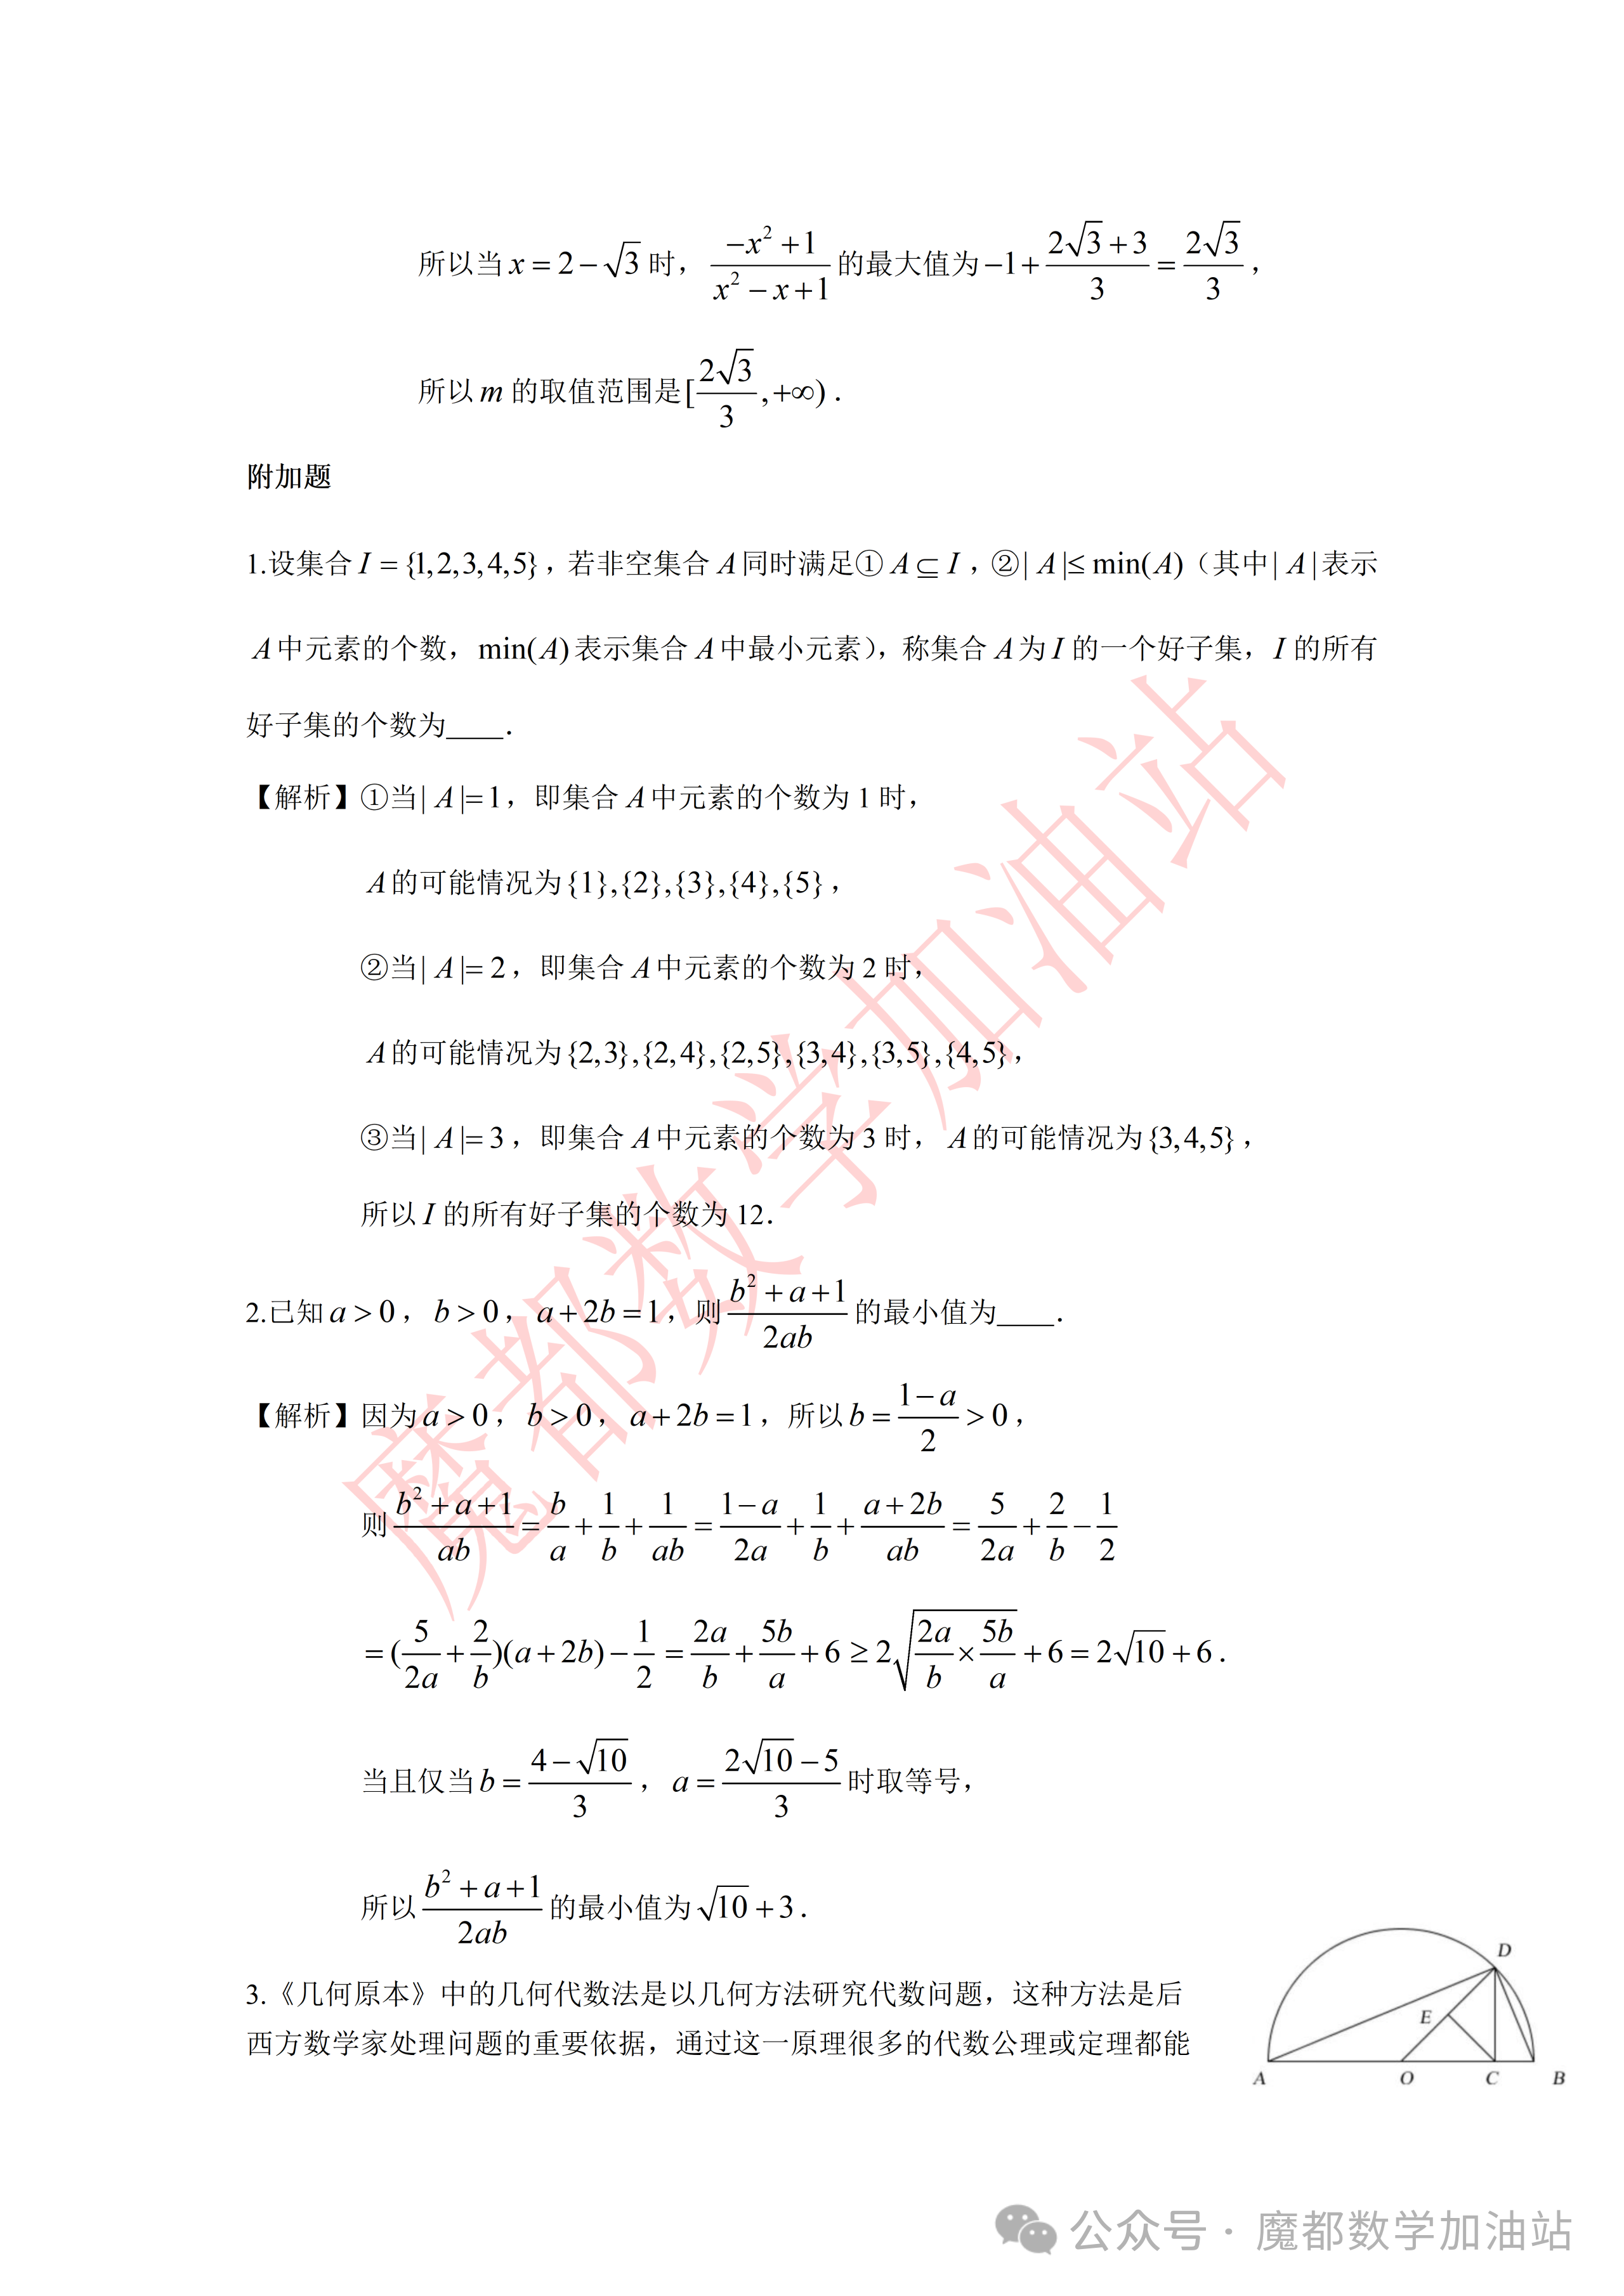
\includegraphics[width=.34\linewidth,trim=1960bp 310bp 90bp 3015bp,clip]{../原图/高一47_七宝中学_抱孩子练习9.26/08.png}
\end{center}

① $\dfrac{a+b}{2}\geqslant\sqrt{ab}$（$a>0$，$b>0$）；
② $a^2+b^2\geqslant2ab$（$a>0$，$b>0$）；
③ $\sqrt{ab}\geqslant\dfrac{2}{\dfrac1a+\dfrac1b}$（$a>0$，$b>0$）；
④ $\sqrt{\dfrac{a^2+b^2}{2}}\geqslant\dfrac{a+b}{2}$（$a>0$，$b>0$）.

\ifanswer
\solbegin
\step{因为 $AC+CB=a+b$，所以 $OD=\dfrac{AB}{2}=\dfrac{AC+CB}{2}=\dfrac{a+b}{2}$；}
\step{由射影定理得 $CD=\sqrt{AC\times CB}=\sqrt{ab}$，又因为 $OD\geqslant CD$，}
\step{所以 $\dfrac{a+b}{2}\geqslant\sqrt{ab}$，故①正确；}
\step{由射影定理得 $CD^2=DE\times OD$，所以 $DE=\dfrac{CD^2}{OD}=\dfrac{ab}{\dfrac{a+b}{2}}=\dfrac{2}{\dfrac1a+\dfrac1b}$，}
\step{又因为 $CD\geqslant DE$，所以 $\sqrt{ab}\geqslant\dfrac{2}{\dfrac1a+\dfrac1b}$，故③正确；}
\step{故该图形可以完成的所有无字证明为①③.}
\solend

\fi

% 注：原卷此处印作等式 $|x^2+a|+|x-a|=|x^2+x|$（在 $x>0$ 时与三角不等式下界等价），本稿曾改写成
% 不等式，现按原卷照录（原卷如此，照录未改）。
\item 若对任意 $x\in[2,3]$，均有 $|x^2+a|+|x-a|=|x^2+x|$，则实数 $a$ 的取值范围为 \blankline[4.4em].

\ifanswer
\solbegin
\step{因为 $|a|+|b|=|a+b|$ 当且仅当 $ab\geqslant0$ 时取等号，}
\step{所以 $(x^2+a)(x-a)\geqslant0$，即 $(a+x^2)(a-x)\leqslant0$，所以 $-x^2\leqslant a\leqslant x$ 恒成立，}
\step{因为 $x\in[2,3]$，所以 $-4\leqslant a\leqslant2$，所以实数 $a$ 的取值范围为 $[-4,2]$.}
\solend

\fi

\end{enumerate}

\end{document}
"
% 紧凑版：xelatex "\def\iscompact{1}% 高一47_七宝中学_抱孩子练习9.26.tex
%   —— 高一上数学“2026-2027 年七宝中学高一上抱孩子练习 9.26”（试卷版/答案版）
% 试卷版：xelatex 高一47_七宝中学_抱孩子练习9.26.tex
% 答案版：xelatex "\def\isanswer{1}% 高一47_七宝中学_抱孩子练习9.26.tex
%   —— 高一上数学“2026-2027 年七宝中学高一上抱孩子练习 9.26”（试卷版/答案版）
% 试卷版：xelatex 高一47_七宝中学_抱孩子练习9.26.tex
% 答案版：xelatex "\def\isanswer{1}\input{高一47_七宝中学_抱孩子练习9.26.tex}"
% 紧凑版：xelatex "\def\iscompact{1}\input{高一47_七宝中学_抱孩子练习9.26.tex}"
%
% 原始材料是微信公众号图文（公众号“魔都数学加油站”连载“27学年高一47”，署名“破晓”，
% 2026-10-02 17:56 发布，原文标题“27学年高一47——2026-2027年上海市七宝中学高一上抱孩子练习9.26”，
% 原文链接 https://mp.weixin.qq.com/s/mhkyDwjn7QFP_Z_NOcPkQA），正文为 9 张 PNG 页。
% 第 1—7、9 页分辨率为 4762×6735，第 8 页为 2560×3620；均按原图逐页核对。
% 原卷文字、选项、答案与解析均照录；粉色斜水印及灰色公众号页脚属水印/页脚，未录入。
%
% 卷首标题：原卷印作“2026-2027 年七宝中学高一上抱孩子练习 9.26”（公众号标题里的“上海市”
% 三字卷面标题行没有，本稿照卷面），年份区间按全稿惯例排 en dash，作业名保留原卷日期“9.26”。
% 原卷未印独立副标题；本稿按“知识模块”口径补出“集合与常用逻辑用语、不等式”。
%
% 与原卷的排版差异：
%   ① 原卷分“一、填空题”“二、选择题”“三、解答题”“附加题”四节；前三节题号为 3—16，
%      分别有 8 道填空、3 道选择、3 道解答；附加题另起 1—4 编号；
%   ② 原卷题下直接印答案/解析，本稿按全稿统一收进答案版；填空横线采用统一长度；
%   ③ 原卷未印副标题，本稿按“知识模块”口径补出（见卷首标题）；
%   ④ 全卷只有附加题第 3 题带图，直接从原卷第 8 页裁取。
%
% 原卷存疑（照录未改，见源码中该处上方注释）：
%   ① 第 9 题集合 C 的条件原文作“C={x|y=..., x 是整数}”，其中 y 未在集合描述中定义；
%      本稿照录原记号，未代换为 x。
%   ② 附加题第 3 题原文作“后西方数学家”，措辞存疑（疑漏“世”字）；本稿照录未改。
%
\documentclass[a4paper,11pt]{article}
\usepackage{common}

\begin{document}

\examtitlest[3]{2026--2027 年七宝中学高一上抱孩子练习 9.26}{集合与常用逻辑用语、不等式}

\bigsec{一、填空题}

\begin{enumerate}
\setcounter{enumi}{2}

\item 若不等式 $|x|<a$ 的一个充分条件为 $0<x<1$，则实数 $a$ 的取值范围是 \blankline[4.4em].

\ifanswer
\solbegin
\step{由 $|x|<a$ 得到 $-a<x<a$，}
\step{又不等式 $|x|<a$ 的一个充分条件为 $0<x<1$，所以 $a\geqslant1$.}
\solend

\fi

\item 已知命题“$\exists x\in\R$，使 $4x^2+(a-2)x+\dfrac14=0$”是假命题，则实数 $a$ 的取值范围是 \blankline[4.4em].

\ifanswer
\solbegin
% 注：原卷首句作“为真命题”（先按命题为真推出 $\Delta\geqslant0$，再由其为假得 $0<a<4$），原卷如此，照录未改。
\step{命题 $\exists x\in\R$，使 $4x^2+(a-2)x+\dfrac14=0$ 为真命题，}
\step{则 $\Delta=(a-2)^2-4\times4\times\dfrac14=a^2-4a\geqslant0$，解得 $a\leqslant0$ 或 $a\geqslant4$，}
\step{而命题“$\exists x\in\R$，使 $4x^2+(a-2)x+\dfrac14=0$”是假命题，则 $0<a<4$，}
\step{所以实数 $a$ 的取值范围是 $\{a\mid0<a<4\}$.}
\solend

\fi

\item 已知集合 $A=\{x\mid(a-1)x^2+3x-2=0\}$ 有且仅有两个子集，则实数 $a=$ \blankline[4.4em].

\ifanswer
\solbegin
\step{集合 $A=\{x\mid(a-1)x^2+3x-2=0\}$ 有且仅有两个不同的子集，}
\step{所以 $a-1=0$ 或 $\begin{cases}a-1\neq0\\\Delta=9+8(a-1)=0\end{cases}$，解得实数 $a=1$ 或 $a=-\dfrac18$.}
\solend

\fi

\item 已知函数 $y=x^2+bx+3$（其中 $b$ 是实数）中，$y$ 的取值范围是 $[0,+\infty)$，若关于 $x$ 的不等式 $x^2+bx+3<c$ 的解集为 $m-8<x<m$，则实数 $c$ 的值为 \blankline[4.4em].

\ifanswer
\solbegin
\step{因为 $y$ 的取值范围是 $[0,+\infty)$，所以 $\Delta=b^2-12=0$，解得 $b^2=12$，}
\step{因为不等式 $x^2+bx+3<c$ 的解集为 $m-8<x<m$，}
\step{令 $x^2+bx+3=c$，即 $x^2+bx+3-c=0$，方程的两根为 $x_1=m-8$，$x_2=m$，}
\step{所以 $|x_2-x_1|=\sqrt{(x_1+x_2)^2-4x_1x_2}=\sqrt{b^2-4(3-c)}=8$，即 $\sqrt{12-4(3-c)}=8$，}
\step{且判别式 $\Delta=b^2-4(3-c)=12-4(3-c)>0$，解得 $c=16$.}
\solend

\fi

\item 关于 $x$ 的不等式 $|x-1|+|x+1|\geqslant a$ 的解集为 $\R$，则实数 $a$ 的取值范围为 \blankline[4.4em].

\ifanswer
\solbegin
\step{因为 $|x-1|+|x+1|\geqslant|x-1-(x+1)|=2$，}
\step{若关于 $x$ 的不等式 $|x-1|+|x+1|\geqslant a$ 的解集为 $\R$，则实数 $a$ 的取值范围为 $a\leqslant2$.}
\solend

\fi

\item 已知 $m>0$，$xy>0$，当 $x+y=2$ 时，不等式 $\dfrac2x+\dfrac my\geqslant4$ 恒成立，则 $m$ 的取值范围是 \blankline[4.4em].

\ifanswer
\solbegin
\step{因为 $m>0$，$xy>0$，$x+y=2$，}
\step{所以 $\dfrac2x+\dfrac my=\dfrac12(x+y)\left(\dfrac2x+\dfrac my\right)
=\dfrac12\left(m+2+\dfrac{2y}{x}+\dfrac{mx}{y}\right)$}
\step{$\geqslant\dfrac12\left(m+2+2\sqrt{\dfrac{2y}{x}\cdot\dfrac{mx}{y}}\right)=\dfrac12\left(m+2+2\sqrt{2m}\right)$，}
\step{当且仅当 $\dfrac{2y}{x}=\dfrac{mx}{y}$，即 $y^2=\dfrac{mx^2}{2}$ 时取等号.}
\step{因为不等式 $\dfrac2x+\dfrac my\geqslant4$ 恒成立，所以 $\dfrac12(m+2+2\sqrt{2m})\geqslant4$，}
\step{整理得 $(\sqrt m+3\sqrt2)(\sqrt m-\sqrt2)\geqslant0$，解得 $\sqrt m\geqslant\sqrt2$，即 $m\geqslant2$，}
\step{所以 $m$ 的取值范围为 $[2,+\infty)$.}
\solend

\fi

\item 已知全集为 $\R$，集合 $D=\{x\mid x^2-ax+a^2-19=0\}$，
$B=\{y\mid y=-x^2+2x+2,\ y\text{ 是正整数}\}$，
% 注：本题集合 C 的条件原文作“C={x|y=..., x 是整数}”，其中 y 未在集合描述中定义；照录未改。
集合 $C=\left\{x\mathrel{\Big|}y=\sqrt{\dfrac{2-x}{x+1}},\ x\text{ 是整数}\right\}$，且集合 $D$ 满足 $D\cap B\neq\varnothing$，$\overline{D}\cup\overline{C}=\R$，则实数 $a$ 的值是 \blankline[4.4em].

\ifanswer
\solbegin
\step{集合 $B=\{y\mid y=-x^2+2x+2,\ y\text{ 是正整数}\}=\{1,2,3\}$，}
\step{集合 $C=\left\{x\mathrel{\Big|}y=\sqrt{\dfrac{2-x}{x+1}},\ x\text{ 是整数}\right\}=\{0,1,2\}$，}
\step{集合 $D=\{x\mid x^2-ax+a^2-19=0\}$ 且集合 $D$ 满足 $D\cap B\neq\varnothing$，$\overline{D}\cup\overline{C}=\R$，}
\step{所以 $3\in D$，解得 $a=5$ 或 $a=-2$，}
\step{经检验，$a=5$ 不符合 $\overline{D}\cup\overline{C}=\R$，舍去，$a=-2$ 满足题意，即 $a=-2$.}
\solend

\fi

% 注：本题解析中，$a=\pm2\sqrt2$ 时 $B$ 的二重根按 $-\dfrac a2$ 应为 $\mp\sqrt2$，原卷印作 $\mp2\sqrt2$、
% $-\dfrac{3\sqrt2}4$，$C(B)=3$ 的计算也随之按原卷保留（原卷如此，照录未改）。
\item 用 $C(A)$ 表示非空集合 $A$ 中的元素的个数，定义 $A*B=|C(A)-C(B)|$，已知集合 $A$ 有三个真子集，
$B=\{x\mid(ax^2+3x)(x^2+ax+2)=0,\ x\in\R\}$，若 $A*B=1$，设实数 $a$ 所有可能取值构成集合 $S$，则 $C(S)=$ \blankline[4.4em].

\ifanswer
\solbegin
\step{集合 $A$ 有三个真子集，则集合 $A$ 中有 $2$ 个元素，则 $C(A)=2$，}
\step{由 $A*B=1$，得 $C(B)=1$ 或 $3$，}
\step{即方程 $(ax^2+3x)\cdot(x^2+ax+2)=0$ 有一个根或 $3$ 个根；}
\step{若 $(ax^2+3x)\cdot(x^2+ax+2)=0$，则必有 $ax^2+3x=0$ 或 $x^2+ax+2=0$，}
\step{若 $ax^2+3x=0$，则 $x=0$ 或 $ax+3=0$，}
\step{当 $a=0$ 时，$B=\{0\}$，$C(B)=1$，符合题意；}
\step{当 $a\neq0$ 时，$ax^2+3x=0$ 对应的根为 $0$ 和 $-\dfrac3a$；}
\step{故①需 $x^2+ax+2=0$ 有两等根且根不为 $0$ 和 $-\dfrac3a$，}
\step{当 $\Delta=0$ 时，$a=\pm2\sqrt2$，}
\step{$a=2\sqrt2$，此时 $B=\left\{0,-2\sqrt2,-\dfrac{3\sqrt2}{4}\right\}$，$C(B)=3$，符合题意；}
\step{$a=-2\sqrt2$，此时 $B=\left\{0,2\sqrt2,\dfrac{3\sqrt2}{4}\right\}$，$C(B)=3$，符合题意；}
\step{②当 $-\dfrac3a$ 是 $x^2+ax+2=0$ 的根时，解得 $a=\pm3$；}
\step{$a=3$，此时 $B=\{0,-1,-2\}$，$C(B)=3$，符合题意；}
\step{$a=-3$，此时 $B=\{0,1,2\}$，$C(B)=3$，符合题意；}
\step{综上，$a$ 可取的值为 $0$、$\pm3$、$\pm2\sqrt2$，则 $C(S)=5$.}
\solend

\fi

\end{enumerate}

\bigsec{二、选择题}

\begin{enumerate}
\setcounter{enumi}{10}

\item 已知集合 $A=\left\{x\mathrel{\Big|}\dfrac1x<1\right\}$，$B=\{x\mid x^2-2x-3\leqslant0\}$，则 $A\cap B=$\mbox{（\quad）}

\keepwithprev
A. $\{x\mid1<x\leqslant3\}$\qquad B. $\{x\mid1\leqslant x\leqslant3\text{ 或 }-1\leqslant x<0\}$

C. $\{x\mid-1\leqslant x<0\}$\qquad D. $\{x\mid1<x\leqslant3\text{ 或 }-1\leqslant x<0\}$

\ans{$D$}

% 注：原卷本题只有题干＋选项（答案印在括号内），没有解析；此处照录原卷的"无解析"状态，不排解析。
\item 使 $x(y-2)=0$ 成立的一个充分条件是\mbox{（\quad）}

\keepwithprev
A. $x^2+(y-2)^2=0$\qquad B. $(x-2)^2+y^2=0$

C. $x^2+y^2=1$\qquad D. $x+y-2=0$

\ans{$A$}

\ifanswer
\solbegin
\step{对于 $A$：若 $x^2+(y-2)^2=0$，则 $x=0$ 且 $y=2$，此时 $x(y-2)=0$ 成立，}
\step{即充分性成立.}
\step{若 $x(y-2)=0$，则 $x=0$ 或 $y=2$，当 $x=0$，$y=3$ 时，$x^2+(y-2)^2=0$ 不成立，}
\step{即必要性不成立，}
\step{故 $x^2+(y-2)^2=0$ 是 $x(y-2)=0$ 成立的充分不必要条件；}
\step{对于 $B$：$(x-2)^2+y^2=0$，则 $x=2$ 且 $y=0$，此时 $x(y-2)=0$ 不成立，}
\step{即充分性不成立；}
\step{对于 $C$：$x^2+y^2=1$，此时 $x(y-2)=0$ 不一定成立，即充分性不成立；}
\step{对于 $D$：$x+y-2=0$，此时 $x(y-2)=0$ 不一定成立，即充分性不成立.}
\step{故选 $A$.}
\solend

\fi

\item 已知 $a$、$b$、$c\in\R$，若关于 $x$ 的不等式 $0\leqslant x+\dfrac ax+b\leqslant\dfrac cx-1$ 的解集为 $[x_1,x_2]\cup\{x_3\}$（$x_3>x_2>x_1>0$），则\mbox{（\quad）}

\keepwithprev
A. 不存在有序数组 $(a,b,c)$，使得 $x_2-x_1=1$

B. 存在唯一有序数组 $(a,b,c)$，使得 $x_2-x_1=1$

C. 有且只有两组有序数组 $(a,b,c)$，使得 $x_2-x_1=1$

D. 存在无穷多组有序数组 $(a,b,c)$，使得 $x_2-x_1=1$

\ans{$D$}

\ifanswer
\solbegin
\step{因为不等式 $0\leqslant x+\dfrac ax+b\leqslant\dfrac cx-1$ 的解集为 $[x_1,x_2]\cup\{x_3\}$（$x_3>x_2>x_1>0$），}
\step{所以 $0\leqslant x^2+bx+a\leqslant c-x$ 在 $[x_1,x_2]\cup\{x_3\}$ 上成立，}
\step{假设 $x_1=m$，$x_2=m+1$，$x_3=n$，}
\step{则 $c-n=0=n^2+bn+a$，由 $x_3$ 为一个独立的数得出，}
\step{所以 $n=c$，且 $m+1$ 与 $n$ 为方程 $x^2+bx+a=0$ 的两个根，}
\step{因为 $x_3>x_2>x_1>0$，所以 $-b=m+n+1=m+c+1$，$a=mn+n=mc+c$，}
\step{所以 $b=-m-c-1$，}
\step{且点 $(x_1,x_1^2+bx_1+a)$ 为 $y=x^2+bx+a$ 与 $y=c-x$ 的左交点，}
\step{所以 $m^2+bm+a=c-m$ 且 $b=-m-c-1$，$a=mc+c$，}
% 注：原卷此行的末句作“所以 $c-m=c-m$ 恒成立”（未写成 $x_2-x_1=1$），原卷如此，照录未改。
\step{故 $m^2+bm+a=m^2-m^2-mc-m+mc+c=c-m$，所以 $c-m=c-m$ 恒成立，}
\step{所以不论 $a$、$b$、$c$ 取何值，$x_2-x_1=1$ 恒成立，}
\step{即存在无穷多组有序数组 $(a,b,c)$，使得 $x_2-x_1=1$，}
\step{故选项 $A$、$B$、$C$ 错误，选项 $D$ 正确. 故选 $D$.}
\solend

\fi

\end{enumerate}

\bigsec{三、解答题}

\begin{enumerate}
\setcounter{enumi}{13}

\item 设正实数 $x$、$y$，满足 $2x+y=1$，求：

\begin{enumerate}[label=(\arabic*)]
\item $\sqrt{2x}+\sqrt y$ 的最大值；
\item $\dfrac2x+\dfrac1y$ 的最小值.
\end{enumerate}

\ifanswer
\solbegin
\stepm{(1)}{对于 $(\sqrt{2x}+\sqrt y)^2=2x+y+2\sqrt{2xy}\leqslant1+1=2$，}
\step{当且仅当 $\sqrt{2x}=\sqrt y$ 时取等号，故 $\sqrt{2x}+\sqrt y$ 的最大值为 $\sqrt2$；}
\stepm{(2)}{$\dfrac2x+\dfrac1y=\left(\dfrac2x+\dfrac1y\right)(2x+y)=5+\dfrac{2y}{x}+\dfrac{2x}{y}\geqslant5+4=9$，}
\step{当且仅当 $\dfrac{2y}{x}=\dfrac{2x}{y}$，即 $x=y=\dfrac13$ 时取等号，故 $\dfrac2x+\dfrac1y$ 的最小值为 $9$.}
\solend

\fi

\ansspace[6]

\item 设 $x_1$、$x_2$ 为关于 $x$ 的方程 $x^2-2(m+2)x+m^2-1=0$ 的两实数根.

\begin{enumerate}[label=(\arabic*)]
\item 若 $x_1$、$x_2$ 满足 $x_1^2+x_2^2=18$，试求 $m$ 的值；
\item 若 $x_1$、$x_2$ 均大于 $0$，求 $m$ 的取值范围.
\end{enumerate}

\ifanswer
\solbegin
\stepm{(1)}{由 $\Delta=4(m+2)^2-4(m^2-1)\geqslant0$，解得 $m\geqslant-\dfrac54$，}
\step{由韦达定理得 $x_1+x_2=2(m+2)$，$x_1x_2=m^2-1$，}
\step{又 $x_1^2+x_2^2=(x_1+x_2)^2-2x_1x_2=4(m+2)^2-2(m^2-1)=18$，}
\step{即 $m^2+8m=0$，解得 $m=0$ 或 $m=-8$（舍），故 $m$ 的值为 $0$；}
% 注：原卷此处作“由（2）得”（对照上一小问，所指应为（1）），原卷如此，照录未改。
\stepm{(2)}{由（2）得 $m\geqslant-\dfrac54$，}
\step{又 $x_1$、$x_2$ 均大于 $0$，则 $\begin{cases}2(m+2)>0\\m^2-1>0\end{cases}$，解得 $\begin{cases}m>-2\\m>1\text{或}m<-1\end{cases}$，}
\step{综上，实数 $m$ 的取值范围为 $\left[-\dfrac54,-1\right)\cup(1,+\infty)$.}
\solend

\fi

\ansspace[6]

\item 已知函数 $f(x)=(m+1)x^2-mx+m-1$（$m\in\R$）.

\begin{enumerate}[label=(\arabic*)]
\item 若不等式 $f(x)<0$ 的解集是空集，求 $m$ 的取值范围；
\item 当 $m>-2$ 时，解不等式 $f(x)\geqslant m$；
\item 若不等式 $f(x)\geqslant0$ 的解集为 $D$，若 $[-1,1]\subseteq D$，求 $m$ 的取值范围.
\end{enumerate}

\ifanswer
\solbegin
\stepm{(1)}{①当 $m+1=0$，即 $m=-1$ 时，$f(x)=x-2$，不合题意；}
\step{②当 $m+1\neq0$，即 $m\neq-1$ 时，$\begin{cases}m+1>0\\\Delta=m^2-4(m+1)(m-1)\leqslant0\end{cases}$，解得 $m\geqslant\dfrac{2\sqrt3}{3}$，}
\step{所以 $m$ 的取值范围是 $\left[\dfrac{2\sqrt3}{3},+\infty\right)$；}
\stepm{(2)}{因为 $f(x)\geqslant m$，所以 $(m+1)x^2-mx-1\geqslant0$，即 $[(m+1)x+1](x-1)\geqslant0$，}
\step{①当 $m+1=0$ 即 $m=-1$ 时，不等式的解集为 $[1,+\infty)$；}
\step{②当 $m+1>0$ 即 $m>-1$ 时，$\left(x+\dfrac1{m+1}\right)(x-1)\geqslant0$，}
\step{因为 $-\dfrac1{m+1}<0$，所以不等式的解集为 $\left(-\infty,-\dfrac1{m+1}\right]\cup[1,+\infty)$；}
\step{③当 $m+1<0$ 即 $-2<m<-1$ 时，$\left(x+\dfrac1{m+1}\right)(x-1)\leqslant0$，}
\step{因为 $-2<m<-1$，所以 $-1<m+1<0$，所以 $-\dfrac1{m+1}>1$，}
\step{所以不等式的解集为 $\left[1,-\dfrac1{m+1}\right]$；}
\stepm{(3)}{不等式 $f(x)\geqslant0$ 的解集为 $D$，若 $[-1,1]\subseteq D$，}
\step{即对任意的 $x\in[-1,1]$，不等式 $(m+1)x^2-mx+m-1\geqslant0$ 恒成立，}
\step{即 $m(x^2-x+1)\geqslant-x^2+1$ 恒成立，}
\step{因为 $x^2-x+1>0$ 恒成立，所以 $m\geqslant\dfrac{-x^2+1}{x^2-x+1}=-1+\dfrac{2-x}{x^2-x+1}$ 恒成立，}
\step{设 $t=2-x$，则 $t\in[1,3]$，$x=2-t$，}
\step{则 $\dfrac{2-x}{x^2-x+1}=\dfrac{t}{(2-t)^2-(2-t)+1}=\dfrac{t}{t^2-3t+3}=\dfrac1{t+\dfrac3t-3}$，}
\step{因为 $t+\dfrac3t\geqslant2\sqrt3$，当且仅当 $t=\sqrt3$ 时取等号，}
\step{所以 $\dfrac{2-x}{x^2-x+1}\leqslant\dfrac1{2\sqrt3-3}=\dfrac{2\sqrt3+3}{3}$，当且仅当 $x=2-\sqrt3$ 时取等号，}
\step{所以当 $x=2-\sqrt3$ 时，$\dfrac{-x^2+1}{x^2-x+1}$ 的最大值为 $-1+\dfrac{2\sqrt3+3}{3}=\dfrac{2\sqrt3}{3}$，}
\step{所以 $m$ 的取值范围是 $\left[\dfrac{2\sqrt3}{3},+\infty\right)$.}
\solend

\fi

\ansspace[8]

\end{enumerate}

\bigsec{附加题}

\begin{enumerate}

\item 设集合 $I=\{1,2,3,4,5\}$，若非空集合 $A$ 同时满足① $A\subseteq I$，② $|A|\leqslant\min(A)$（其中 $|A|$ 表示集合 $A$ 中元素的个数，$\min(A)$ 表示集合 $A$ 中最小元素），称集合 $A$ 为 $I$ 的一个好子集，$I$ 所有好子集的个数为 \blankline[4.4em].

\ifanswer
\solbegin
\step{①当 $|A|=1$，即集合 $A$ 中元素的个数为 $1$ 时，}
\step{$A$ 的可能情况为 $\{1\}$、$\{2\}$、$\{3\}$、$\{4\}$、$\{5\}$，}
\step{②当 $|A|=2$，即集合 $A$ 中元素的个数为 $2$ 时，}
\step{$A$ 的可能情况为 $\{2,3\}$、$\{2,4\}$、$\{2,5\}$、$\{3,4\}$、$\{3,5\}$、$\{4,5\}$，}
\step{③当 $|A|=3$，即集合 $A$ 中元素的个数为 $3$ 时，$A$ 的可能情况为 $\{3,4,5\}$，}
\step{所以 $I$ 的所有好子集的个数为 $12$.}
\solend

\fi

\item 已知 $a>0$，$b>0$，$a+2b=1$，则 $\dfrac{b^2+a+1}{2ab}$ 的最小值为 \blankline[4.4em].

\ifanswer
\solbegin
\step{因为 $a>0$，$b>0$，$a+2b=1$，所以 $b=\dfrac{1-a}{2}>0$，}
\step{则 $\dfrac{b^2+a+1}{ab}=\dfrac ba+\dfrac1b+\dfrac1{ab}=\dfrac{1-a}{2a}+\dfrac1b+\dfrac{a+2b}{ab}=\dfrac5{2a}+\dfrac2b-\dfrac12$}
\step{$=\left(\dfrac5{2a}+\dfrac2b\right)(a+2b)-\dfrac12=\dfrac{2a}{b}+\dfrac{5b}{a}+6\geqslant2\sqrt{\dfrac{2a}{b}\times\dfrac{5b}{a}}+6=2\sqrt{10}+6$.}
\step{当且仅当 $b=\dfrac{4-\sqrt{10}}{3}$，$a=\dfrac{2\sqrt{10}-5}{3}$ 时取等号，}
\step{所以 $\dfrac{b^2+a+1}{2ab}$ 的最小值为 $\sqrt{10}+3$.}
\solend

\fi

% 注：本题原文作“后西方数学家”，措辞存疑（疑漏“世”字）；照录未改，见文件头“原卷存疑”②。
% 又原文作"很多的代数公理或定理都能够通过图形实现证明"（"公理"疑为"公式"笔误）、
% "连结 OD,AD,BD"，均原卷如此，照录未改。
\item 《几何原本》中的几何代数法是以几何方法研究代数问题，这种方法是后西方数学家处理问题的重要依据，通过这一原理很多的代数公理或定理都能够通过图形实现证明，也称之为无字证明，现有图形如图所示，$C$ 为线段 $AB$ 上的点，且 $AC=a$，$BC=b$，$O$ 为 $AB$ 的中点，以 $AB$ 为直径作半圆，过点 $C$ 作 $AB$ 的垂线交半圆于 $D$，连结 $OD,AD,BD$，过点 $C$ 作 $OD$ 的垂线，垂足为 $E$，若不添加辅助线，则该图形可以完成的所有无字证明为 \blankline[4.4em]（填写序号）.

\begin{center}
% 插图直接裁自原卷第 8 页，未重绘；用 trim/clip 保留原图与标注。
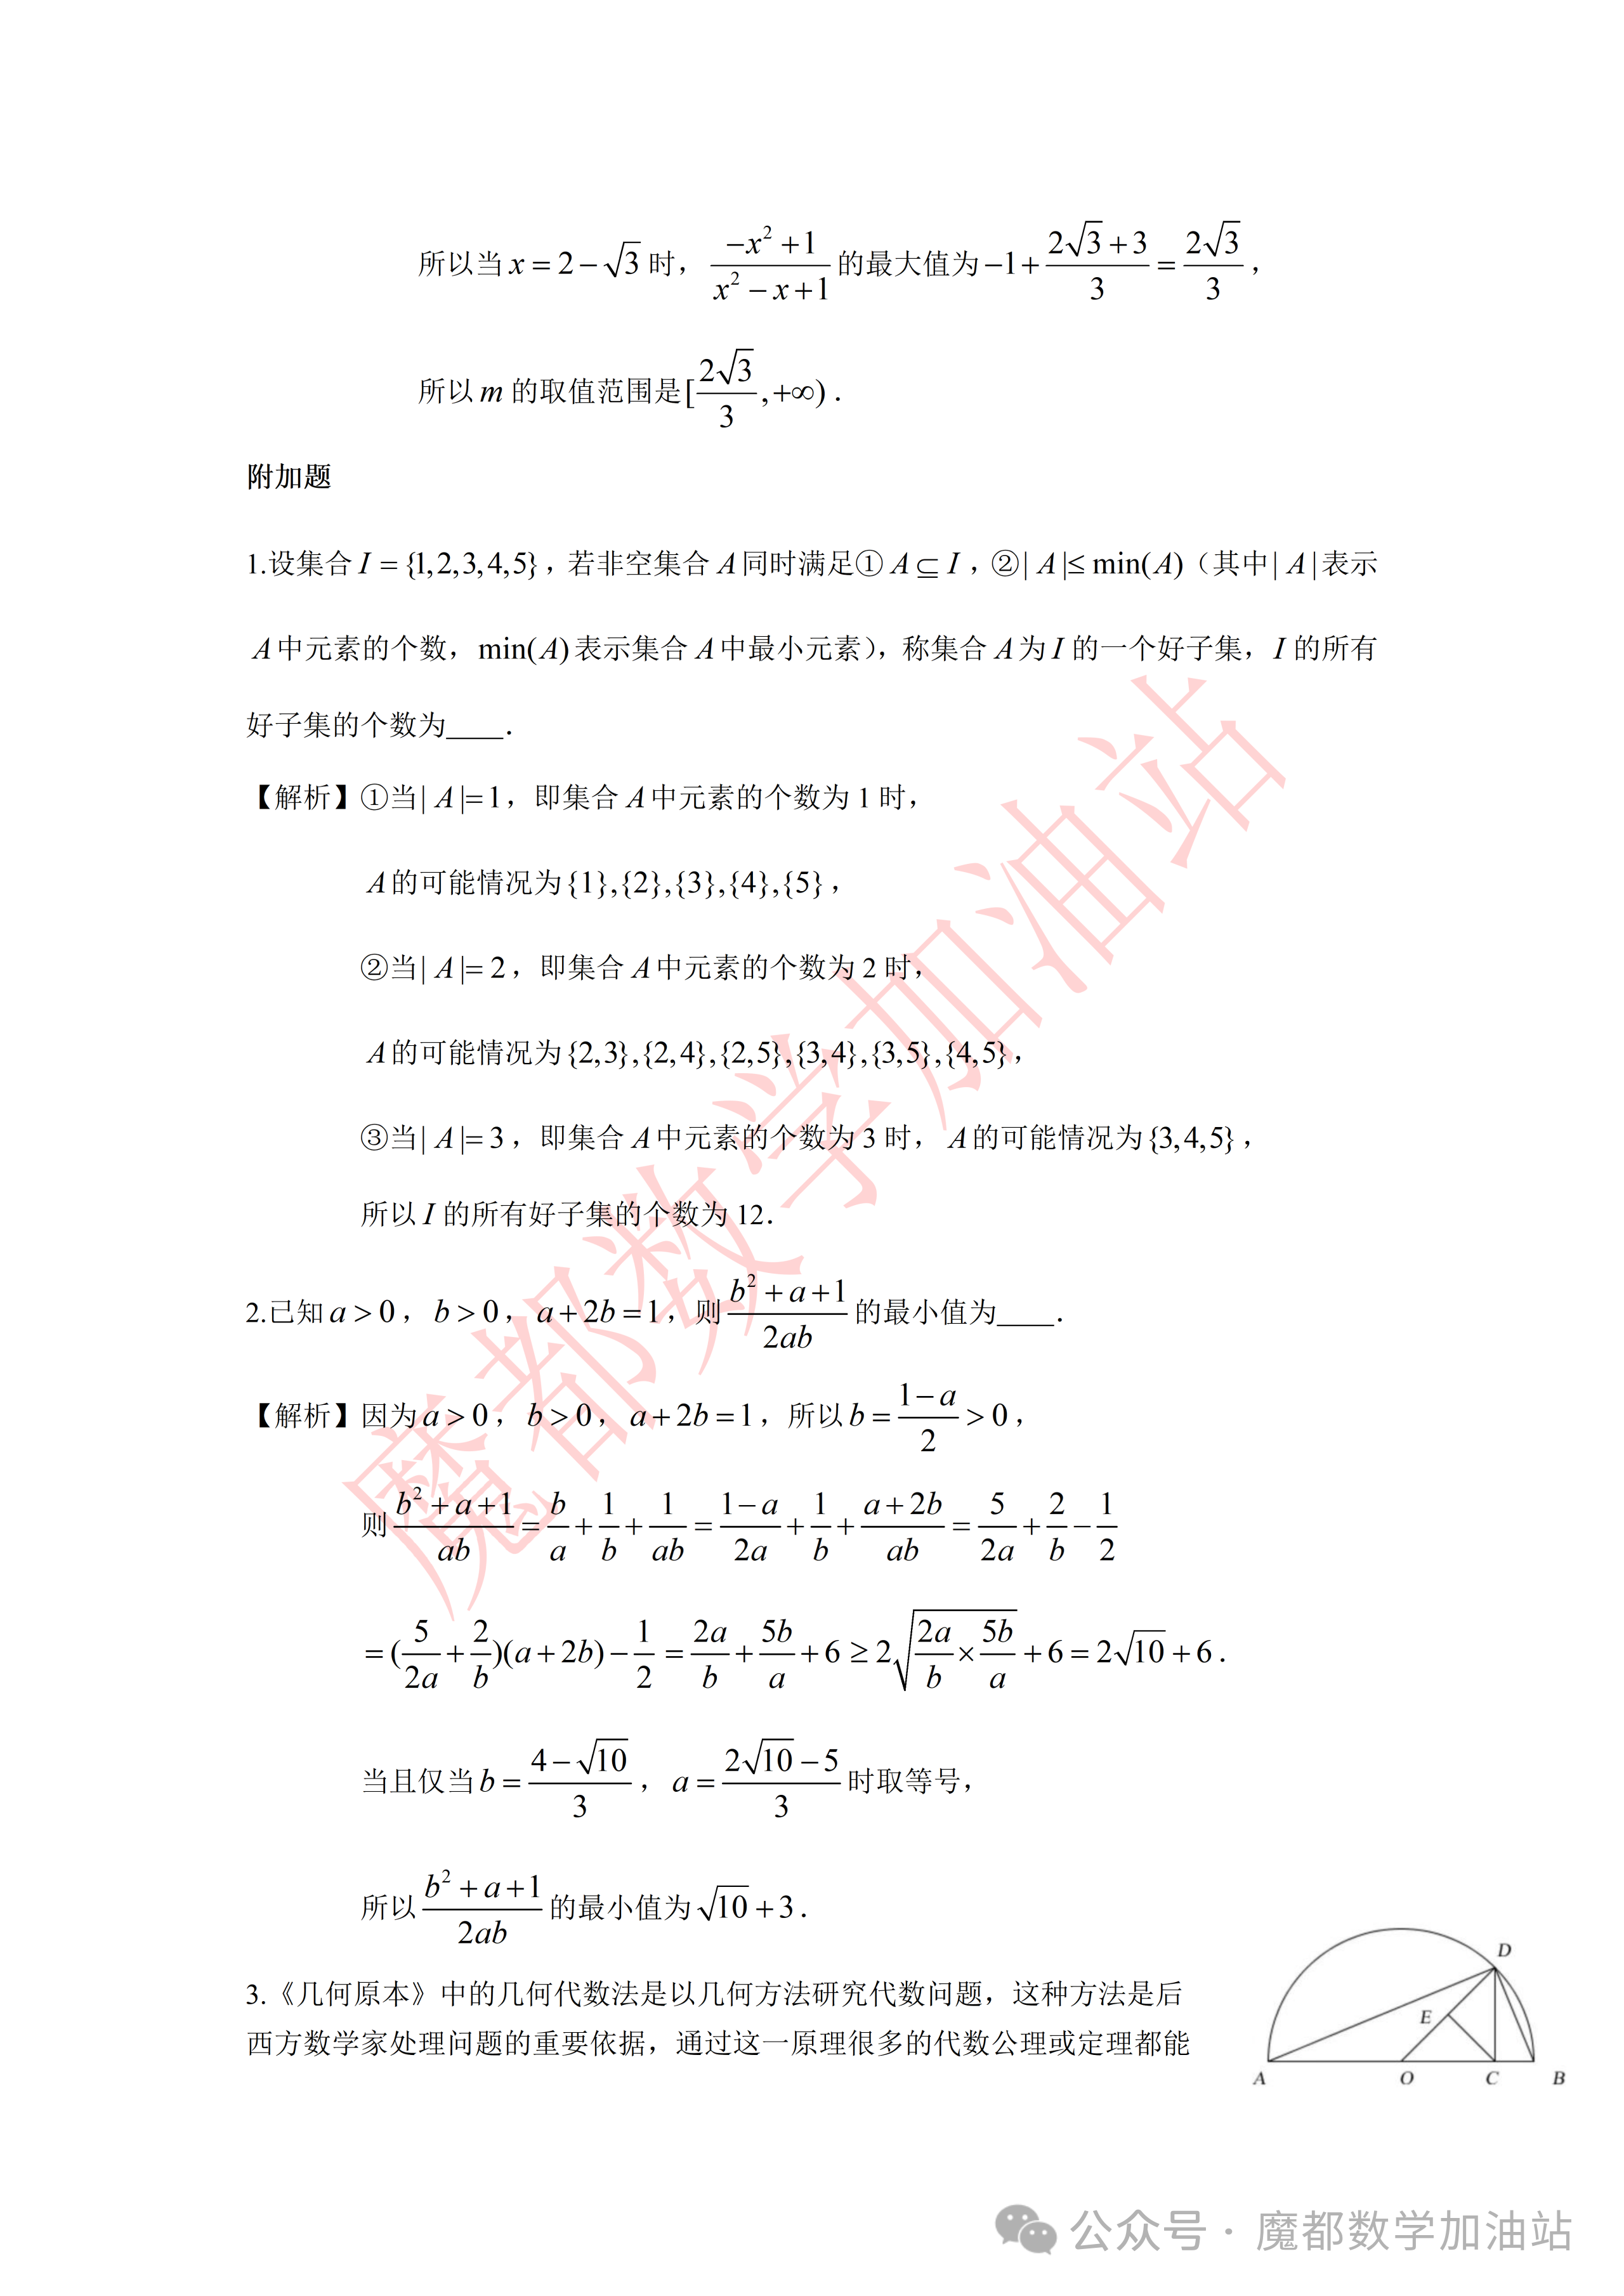
\includegraphics[width=.34\linewidth,trim=1960bp 310bp 90bp 3015bp,clip]{../原图/高一47_七宝中学_抱孩子练习9.26/08.png}
\end{center}

① $\dfrac{a+b}{2}\geqslant\sqrt{ab}$（$a>0$，$b>0$）；
② $a^2+b^2\geqslant2ab$（$a>0$，$b>0$）；
③ $\sqrt{ab}\geqslant\dfrac{2}{\dfrac1a+\dfrac1b}$（$a>0$，$b>0$）；
④ $\sqrt{\dfrac{a^2+b^2}{2}}\geqslant\dfrac{a+b}{2}$（$a>0$，$b>0$）.

\ifanswer
\solbegin
\step{因为 $AC+CB=a+b$，所以 $OD=\dfrac{AB}{2}=\dfrac{AC+CB}{2}=\dfrac{a+b}{2}$；}
\step{由射影定理得 $CD=\sqrt{AC\times CB}=\sqrt{ab}$，又因为 $OD\geqslant CD$，}
\step{所以 $\dfrac{a+b}{2}\geqslant\sqrt{ab}$，故①正确；}
\step{由射影定理得 $CD^2=DE\times OD$，所以 $DE=\dfrac{CD^2}{OD}=\dfrac{ab}{\dfrac{a+b}{2}}=\dfrac{2}{\dfrac1a+\dfrac1b}$，}
\step{又因为 $CD\geqslant DE$，所以 $\sqrt{ab}\geqslant\dfrac{2}{\dfrac1a+\dfrac1b}$，故③正确；}
\step{故该图形可以完成的所有无字证明为①③.}
\solend

\fi

% 注：原卷此处印作等式 $|x^2+a|+|x-a|=|x^2+x|$（在 $x>0$ 时与三角不等式下界等价），本稿曾改写成
% 不等式，现按原卷照录（原卷如此，照录未改）。
\item 若对任意 $x\in[2,3]$，均有 $|x^2+a|+|x-a|=|x^2+x|$，则实数 $a$ 的取值范围为 \blankline[4.4em].

\ifanswer
\solbegin
\step{因为 $|a|+|b|=|a+b|$ 当且仅当 $ab\geqslant0$ 时取等号，}
\step{所以 $(x^2+a)(x-a)\geqslant0$，即 $(a+x^2)(a-x)\leqslant0$，所以 $-x^2\leqslant a\leqslant x$ 恒成立，}
\step{因为 $x\in[2,3]$，所以 $-4\leqslant a\leqslant2$，所以实数 $a$ 的取值范围为 $[-4,2]$.}
\solend

\fi

\end{enumerate}

\end{document}
"
% 紧凑版：xelatex "\def\iscompact{1}% 高一47_七宝中学_抱孩子练习9.26.tex
%   —— 高一上数学“2026-2027 年七宝中学高一上抱孩子练习 9.26”（试卷版/答案版）
% 试卷版：xelatex 高一47_七宝中学_抱孩子练习9.26.tex
% 答案版：xelatex "\def\isanswer{1}\input{高一47_七宝中学_抱孩子练习9.26.tex}"
% 紧凑版：xelatex "\def\iscompact{1}\input{高一47_七宝中学_抱孩子练习9.26.tex}"
%
% 原始材料是微信公众号图文（公众号“魔都数学加油站”连载“27学年高一47”，署名“破晓”，
% 2026-10-02 17:56 发布，原文标题“27学年高一47——2026-2027年上海市七宝中学高一上抱孩子练习9.26”，
% 原文链接 https://mp.weixin.qq.com/s/mhkyDwjn7QFP_Z_NOcPkQA），正文为 9 张 PNG 页。
% 第 1—7、9 页分辨率为 4762×6735，第 8 页为 2560×3620；均按原图逐页核对。
% 原卷文字、选项、答案与解析均照录；粉色斜水印及灰色公众号页脚属水印/页脚，未录入。
%
% 卷首标题：原卷印作“2026-2027 年七宝中学高一上抱孩子练习 9.26”（公众号标题里的“上海市”
% 三字卷面标题行没有，本稿照卷面），年份区间按全稿惯例排 en dash，作业名保留原卷日期“9.26”。
% 原卷未印独立副标题；本稿按“知识模块”口径补出“集合与常用逻辑用语、不等式”。
%
% 与原卷的排版差异：
%   ① 原卷分“一、填空题”“二、选择题”“三、解答题”“附加题”四节；前三节题号为 3—16，
%      分别有 8 道填空、3 道选择、3 道解答；附加题另起 1—4 编号；
%   ② 原卷题下直接印答案/解析，本稿按全稿统一收进答案版；填空横线采用统一长度；
%   ③ 原卷未印副标题，本稿按“知识模块”口径补出（见卷首标题）；
%   ④ 全卷只有附加题第 3 题带图，直接从原卷第 8 页裁取。
%
% 原卷存疑（照录未改，见源码中该处上方注释）：
%   ① 第 9 题集合 C 的条件原文作“C={x|y=..., x 是整数}”，其中 y 未在集合描述中定义；
%      本稿照录原记号，未代换为 x。
%   ② 附加题第 3 题原文作“后西方数学家”，措辞存疑（疑漏“世”字）；本稿照录未改。
%
\documentclass[a4paper,11pt]{article}
\usepackage{common}

\begin{document}

\examtitlest[3]{2026--2027 年七宝中学高一上抱孩子练习 9.26}{集合与常用逻辑用语、不等式}

\bigsec{一、填空题}

\begin{enumerate}
\setcounter{enumi}{2}

\item 若不等式 $|x|<a$ 的一个充分条件为 $0<x<1$，则实数 $a$ 的取值范围是 \blankline[4.4em].

\ifanswer
\solbegin
\step{由 $|x|<a$ 得到 $-a<x<a$，}
\step{又不等式 $|x|<a$ 的一个充分条件为 $0<x<1$，所以 $a\geqslant1$.}
\solend

\fi

\item 已知命题“$\exists x\in\R$，使 $4x^2+(a-2)x+\dfrac14=0$”是假命题，则实数 $a$ 的取值范围是 \blankline[4.4em].

\ifanswer
\solbegin
% 注：原卷首句作“为真命题”（先按命题为真推出 $\Delta\geqslant0$，再由其为假得 $0<a<4$），原卷如此，照录未改。
\step{命题 $\exists x\in\R$，使 $4x^2+(a-2)x+\dfrac14=0$ 为真命题，}
\step{则 $\Delta=(a-2)^2-4\times4\times\dfrac14=a^2-4a\geqslant0$，解得 $a\leqslant0$ 或 $a\geqslant4$，}
\step{而命题“$\exists x\in\R$，使 $4x^2+(a-2)x+\dfrac14=0$”是假命题，则 $0<a<4$，}
\step{所以实数 $a$ 的取值范围是 $\{a\mid0<a<4\}$.}
\solend

\fi

\item 已知集合 $A=\{x\mid(a-1)x^2+3x-2=0\}$ 有且仅有两个子集，则实数 $a=$ \blankline[4.4em].

\ifanswer
\solbegin
\step{集合 $A=\{x\mid(a-1)x^2+3x-2=0\}$ 有且仅有两个不同的子集，}
\step{所以 $a-1=0$ 或 $\begin{cases}a-1\neq0\\\Delta=9+8(a-1)=0\end{cases}$，解得实数 $a=1$ 或 $a=-\dfrac18$.}
\solend

\fi

\item 已知函数 $y=x^2+bx+3$（其中 $b$ 是实数）中，$y$ 的取值范围是 $[0,+\infty)$，若关于 $x$ 的不等式 $x^2+bx+3<c$ 的解集为 $m-8<x<m$，则实数 $c$ 的值为 \blankline[4.4em].

\ifanswer
\solbegin
\step{因为 $y$ 的取值范围是 $[0,+\infty)$，所以 $\Delta=b^2-12=0$，解得 $b^2=12$，}
\step{因为不等式 $x^2+bx+3<c$ 的解集为 $m-8<x<m$，}
\step{令 $x^2+bx+3=c$，即 $x^2+bx+3-c=0$，方程的两根为 $x_1=m-8$，$x_2=m$，}
\step{所以 $|x_2-x_1|=\sqrt{(x_1+x_2)^2-4x_1x_2}=\sqrt{b^2-4(3-c)}=8$，即 $\sqrt{12-4(3-c)}=8$，}
\step{且判别式 $\Delta=b^2-4(3-c)=12-4(3-c)>0$，解得 $c=16$.}
\solend

\fi

\item 关于 $x$ 的不等式 $|x-1|+|x+1|\geqslant a$ 的解集为 $\R$，则实数 $a$ 的取值范围为 \blankline[4.4em].

\ifanswer
\solbegin
\step{因为 $|x-1|+|x+1|\geqslant|x-1-(x+1)|=2$，}
\step{若关于 $x$ 的不等式 $|x-1|+|x+1|\geqslant a$ 的解集为 $\R$，则实数 $a$ 的取值范围为 $a\leqslant2$.}
\solend

\fi

\item 已知 $m>0$，$xy>0$，当 $x+y=2$ 时，不等式 $\dfrac2x+\dfrac my\geqslant4$ 恒成立，则 $m$ 的取值范围是 \blankline[4.4em].

\ifanswer
\solbegin
\step{因为 $m>0$，$xy>0$，$x+y=2$，}
\step{所以 $\dfrac2x+\dfrac my=\dfrac12(x+y)\left(\dfrac2x+\dfrac my\right)
=\dfrac12\left(m+2+\dfrac{2y}{x}+\dfrac{mx}{y}\right)$}
\step{$\geqslant\dfrac12\left(m+2+2\sqrt{\dfrac{2y}{x}\cdot\dfrac{mx}{y}}\right)=\dfrac12\left(m+2+2\sqrt{2m}\right)$，}
\step{当且仅当 $\dfrac{2y}{x}=\dfrac{mx}{y}$，即 $y^2=\dfrac{mx^2}{2}$ 时取等号.}
\step{因为不等式 $\dfrac2x+\dfrac my\geqslant4$ 恒成立，所以 $\dfrac12(m+2+2\sqrt{2m})\geqslant4$，}
\step{整理得 $(\sqrt m+3\sqrt2)(\sqrt m-\sqrt2)\geqslant0$，解得 $\sqrt m\geqslant\sqrt2$，即 $m\geqslant2$，}
\step{所以 $m$ 的取值范围为 $[2,+\infty)$.}
\solend

\fi

\item 已知全集为 $\R$，集合 $D=\{x\mid x^2-ax+a^2-19=0\}$，
$B=\{y\mid y=-x^2+2x+2,\ y\text{ 是正整数}\}$，
% 注：本题集合 C 的条件原文作“C={x|y=..., x 是整数}”，其中 y 未在集合描述中定义；照录未改。
集合 $C=\left\{x\mathrel{\Big|}y=\sqrt{\dfrac{2-x}{x+1}},\ x\text{ 是整数}\right\}$，且集合 $D$ 满足 $D\cap B\neq\varnothing$，$\overline{D}\cup\overline{C}=\R$，则实数 $a$ 的值是 \blankline[4.4em].

\ifanswer
\solbegin
\step{集合 $B=\{y\mid y=-x^2+2x+2,\ y\text{ 是正整数}\}=\{1,2,3\}$，}
\step{集合 $C=\left\{x\mathrel{\Big|}y=\sqrt{\dfrac{2-x}{x+1}},\ x\text{ 是整数}\right\}=\{0,1,2\}$，}
\step{集合 $D=\{x\mid x^2-ax+a^2-19=0\}$ 且集合 $D$ 满足 $D\cap B\neq\varnothing$，$\overline{D}\cup\overline{C}=\R$，}
\step{所以 $3\in D$，解得 $a=5$ 或 $a=-2$，}
\step{经检验，$a=5$ 不符合 $\overline{D}\cup\overline{C}=\R$，舍去，$a=-2$ 满足题意，即 $a=-2$.}
\solend

\fi

% 注：本题解析中，$a=\pm2\sqrt2$ 时 $B$ 的二重根按 $-\dfrac a2$ 应为 $\mp\sqrt2$，原卷印作 $\mp2\sqrt2$、
% $-\dfrac{3\sqrt2}4$，$C(B)=3$ 的计算也随之按原卷保留（原卷如此，照录未改）。
\item 用 $C(A)$ 表示非空集合 $A$ 中的元素的个数，定义 $A*B=|C(A)-C(B)|$，已知集合 $A$ 有三个真子集，
$B=\{x\mid(ax^2+3x)(x^2+ax+2)=0,\ x\in\R\}$，若 $A*B=1$，设实数 $a$ 所有可能取值构成集合 $S$，则 $C(S)=$ \blankline[4.4em].

\ifanswer
\solbegin
\step{集合 $A$ 有三个真子集，则集合 $A$ 中有 $2$ 个元素，则 $C(A)=2$，}
\step{由 $A*B=1$，得 $C(B)=1$ 或 $3$，}
\step{即方程 $(ax^2+3x)\cdot(x^2+ax+2)=0$ 有一个根或 $3$ 个根；}
\step{若 $(ax^2+3x)\cdot(x^2+ax+2)=0$，则必有 $ax^2+3x=0$ 或 $x^2+ax+2=0$，}
\step{若 $ax^2+3x=0$，则 $x=0$ 或 $ax+3=0$，}
\step{当 $a=0$ 时，$B=\{0\}$，$C(B)=1$，符合题意；}
\step{当 $a\neq0$ 时，$ax^2+3x=0$ 对应的根为 $0$ 和 $-\dfrac3a$；}
\step{故①需 $x^2+ax+2=0$ 有两等根且根不为 $0$ 和 $-\dfrac3a$，}
\step{当 $\Delta=0$ 时，$a=\pm2\sqrt2$，}
\step{$a=2\sqrt2$，此时 $B=\left\{0,-2\sqrt2,-\dfrac{3\sqrt2}{4}\right\}$，$C(B)=3$，符合题意；}
\step{$a=-2\sqrt2$，此时 $B=\left\{0,2\sqrt2,\dfrac{3\sqrt2}{4}\right\}$，$C(B)=3$，符合题意；}
\step{②当 $-\dfrac3a$ 是 $x^2+ax+2=0$ 的根时，解得 $a=\pm3$；}
\step{$a=3$，此时 $B=\{0,-1,-2\}$，$C(B)=3$，符合题意；}
\step{$a=-3$，此时 $B=\{0,1,2\}$，$C(B)=3$，符合题意；}
\step{综上，$a$ 可取的值为 $0$、$\pm3$、$\pm2\sqrt2$，则 $C(S)=5$.}
\solend

\fi

\end{enumerate}

\bigsec{二、选择题}

\begin{enumerate}
\setcounter{enumi}{10}

\item 已知集合 $A=\left\{x\mathrel{\Big|}\dfrac1x<1\right\}$，$B=\{x\mid x^2-2x-3\leqslant0\}$，则 $A\cap B=$\mbox{（\quad）}

\keepwithprev
A. $\{x\mid1<x\leqslant3\}$\qquad B. $\{x\mid1\leqslant x\leqslant3\text{ 或 }-1\leqslant x<0\}$

C. $\{x\mid-1\leqslant x<0\}$\qquad D. $\{x\mid1<x\leqslant3\text{ 或 }-1\leqslant x<0\}$

\ans{$D$}

% 注：原卷本题只有题干＋选项（答案印在括号内），没有解析；此处照录原卷的"无解析"状态，不排解析。
\item 使 $x(y-2)=0$ 成立的一个充分条件是\mbox{（\quad）}

\keepwithprev
A. $x^2+(y-2)^2=0$\qquad B. $(x-2)^2+y^2=0$

C. $x^2+y^2=1$\qquad D. $x+y-2=0$

\ans{$A$}

\ifanswer
\solbegin
\step{对于 $A$：若 $x^2+(y-2)^2=0$，则 $x=0$ 且 $y=2$，此时 $x(y-2)=0$ 成立，}
\step{即充分性成立.}
\step{若 $x(y-2)=0$，则 $x=0$ 或 $y=2$，当 $x=0$，$y=3$ 时，$x^2+(y-2)^2=0$ 不成立，}
\step{即必要性不成立，}
\step{故 $x^2+(y-2)^2=0$ 是 $x(y-2)=0$ 成立的充分不必要条件；}
\step{对于 $B$：$(x-2)^2+y^2=0$，则 $x=2$ 且 $y=0$，此时 $x(y-2)=0$ 不成立，}
\step{即充分性不成立；}
\step{对于 $C$：$x^2+y^2=1$，此时 $x(y-2)=0$ 不一定成立，即充分性不成立；}
\step{对于 $D$：$x+y-2=0$，此时 $x(y-2)=0$ 不一定成立，即充分性不成立.}
\step{故选 $A$.}
\solend

\fi

\item 已知 $a$、$b$、$c\in\R$，若关于 $x$ 的不等式 $0\leqslant x+\dfrac ax+b\leqslant\dfrac cx-1$ 的解集为 $[x_1,x_2]\cup\{x_3\}$（$x_3>x_2>x_1>0$），则\mbox{（\quad）}

\keepwithprev
A. 不存在有序数组 $(a,b,c)$，使得 $x_2-x_1=1$

B. 存在唯一有序数组 $(a,b,c)$，使得 $x_2-x_1=1$

C. 有且只有两组有序数组 $(a,b,c)$，使得 $x_2-x_1=1$

D. 存在无穷多组有序数组 $(a,b,c)$，使得 $x_2-x_1=1$

\ans{$D$}

\ifanswer
\solbegin
\step{因为不等式 $0\leqslant x+\dfrac ax+b\leqslant\dfrac cx-1$ 的解集为 $[x_1,x_2]\cup\{x_3\}$（$x_3>x_2>x_1>0$），}
\step{所以 $0\leqslant x^2+bx+a\leqslant c-x$ 在 $[x_1,x_2]\cup\{x_3\}$ 上成立，}
\step{假设 $x_1=m$，$x_2=m+1$，$x_3=n$，}
\step{则 $c-n=0=n^2+bn+a$，由 $x_3$ 为一个独立的数得出，}
\step{所以 $n=c$，且 $m+1$ 与 $n$ 为方程 $x^2+bx+a=0$ 的两个根，}
\step{因为 $x_3>x_2>x_1>0$，所以 $-b=m+n+1=m+c+1$，$a=mn+n=mc+c$，}
\step{所以 $b=-m-c-1$，}
\step{且点 $(x_1,x_1^2+bx_1+a)$ 为 $y=x^2+bx+a$ 与 $y=c-x$ 的左交点，}
\step{所以 $m^2+bm+a=c-m$ 且 $b=-m-c-1$，$a=mc+c$，}
% 注：原卷此行的末句作“所以 $c-m=c-m$ 恒成立”（未写成 $x_2-x_1=1$），原卷如此，照录未改。
\step{故 $m^2+bm+a=m^2-m^2-mc-m+mc+c=c-m$，所以 $c-m=c-m$ 恒成立，}
\step{所以不论 $a$、$b$、$c$ 取何值，$x_2-x_1=1$ 恒成立，}
\step{即存在无穷多组有序数组 $(a,b,c)$，使得 $x_2-x_1=1$，}
\step{故选项 $A$、$B$、$C$ 错误，选项 $D$ 正确. 故选 $D$.}
\solend

\fi

\end{enumerate}

\bigsec{三、解答题}

\begin{enumerate}
\setcounter{enumi}{13}

\item 设正实数 $x$、$y$，满足 $2x+y=1$，求：

\begin{enumerate}[label=(\arabic*)]
\item $\sqrt{2x}+\sqrt y$ 的最大值；
\item $\dfrac2x+\dfrac1y$ 的最小值.
\end{enumerate}

\ifanswer
\solbegin
\stepm{(1)}{对于 $(\sqrt{2x}+\sqrt y)^2=2x+y+2\sqrt{2xy}\leqslant1+1=2$，}
\step{当且仅当 $\sqrt{2x}=\sqrt y$ 时取等号，故 $\sqrt{2x}+\sqrt y$ 的最大值为 $\sqrt2$；}
\stepm{(2)}{$\dfrac2x+\dfrac1y=\left(\dfrac2x+\dfrac1y\right)(2x+y)=5+\dfrac{2y}{x}+\dfrac{2x}{y}\geqslant5+4=9$，}
\step{当且仅当 $\dfrac{2y}{x}=\dfrac{2x}{y}$，即 $x=y=\dfrac13$ 时取等号，故 $\dfrac2x+\dfrac1y$ 的最小值为 $9$.}
\solend

\fi

\ansspace[6]

\item 设 $x_1$、$x_2$ 为关于 $x$ 的方程 $x^2-2(m+2)x+m^2-1=0$ 的两实数根.

\begin{enumerate}[label=(\arabic*)]
\item 若 $x_1$、$x_2$ 满足 $x_1^2+x_2^2=18$，试求 $m$ 的值；
\item 若 $x_1$、$x_2$ 均大于 $0$，求 $m$ 的取值范围.
\end{enumerate}

\ifanswer
\solbegin
\stepm{(1)}{由 $\Delta=4(m+2)^2-4(m^2-1)\geqslant0$，解得 $m\geqslant-\dfrac54$，}
\step{由韦达定理得 $x_1+x_2=2(m+2)$，$x_1x_2=m^2-1$，}
\step{又 $x_1^2+x_2^2=(x_1+x_2)^2-2x_1x_2=4(m+2)^2-2(m^2-1)=18$，}
\step{即 $m^2+8m=0$，解得 $m=0$ 或 $m=-8$（舍），故 $m$ 的值为 $0$；}
% 注：原卷此处作“由（2）得”（对照上一小问，所指应为（1）），原卷如此，照录未改。
\stepm{(2)}{由（2）得 $m\geqslant-\dfrac54$，}
\step{又 $x_1$、$x_2$ 均大于 $0$，则 $\begin{cases}2(m+2)>0\\m^2-1>0\end{cases}$，解得 $\begin{cases}m>-2\\m>1\text{或}m<-1\end{cases}$，}
\step{综上，实数 $m$ 的取值范围为 $\left[-\dfrac54,-1\right)\cup(1,+\infty)$.}
\solend

\fi

\ansspace[6]

\item 已知函数 $f(x)=(m+1)x^2-mx+m-1$（$m\in\R$）.

\begin{enumerate}[label=(\arabic*)]
\item 若不等式 $f(x)<0$ 的解集是空集，求 $m$ 的取值范围；
\item 当 $m>-2$ 时，解不等式 $f(x)\geqslant m$；
\item 若不等式 $f(x)\geqslant0$ 的解集为 $D$，若 $[-1,1]\subseteq D$，求 $m$ 的取值范围.
\end{enumerate}

\ifanswer
\solbegin
\stepm{(1)}{①当 $m+1=0$，即 $m=-1$ 时，$f(x)=x-2$，不合题意；}
\step{②当 $m+1\neq0$，即 $m\neq-1$ 时，$\begin{cases}m+1>0\\\Delta=m^2-4(m+1)(m-1)\leqslant0\end{cases}$，解得 $m\geqslant\dfrac{2\sqrt3}{3}$，}
\step{所以 $m$ 的取值范围是 $\left[\dfrac{2\sqrt3}{3},+\infty\right)$；}
\stepm{(2)}{因为 $f(x)\geqslant m$，所以 $(m+1)x^2-mx-1\geqslant0$，即 $[(m+1)x+1](x-1)\geqslant0$，}
\step{①当 $m+1=0$ 即 $m=-1$ 时，不等式的解集为 $[1,+\infty)$；}
\step{②当 $m+1>0$ 即 $m>-1$ 时，$\left(x+\dfrac1{m+1}\right)(x-1)\geqslant0$，}
\step{因为 $-\dfrac1{m+1}<0$，所以不等式的解集为 $\left(-\infty,-\dfrac1{m+1}\right]\cup[1,+\infty)$；}
\step{③当 $m+1<0$ 即 $-2<m<-1$ 时，$\left(x+\dfrac1{m+1}\right)(x-1)\leqslant0$，}
\step{因为 $-2<m<-1$，所以 $-1<m+1<0$，所以 $-\dfrac1{m+1}>1$，}
\step{所以不等式的解集为 $\left[1,-\dfrac1{m+1}\right]$；}
\stepm{(3)}{不等式 $f(x)\geqslant0$ 的解集为 $D$，若 $[-1,1]\subseteq D$，}
\step{即对任意的 $x\in[-1,1]$，不等式 $(m+1)x^2-mx+m-1\geqslant0$ 恒成立，}
\step{即 $m(x^2-x+1)\geqslant-x^2+1$ 恒成立，}
\step{因为 $x^2-x+1>0$ 恒成立，所以 $m\geqslant\dfrac{-x^2+1}{x^2-x+1}=-1+\dfrac{2-x}{x^2-x+1}$ 恒成立，}
\step{设 $t=2-x$，则 $t\in[1,3]$，$x=2-t$，}
\step{则 $\dfrac{2-x}{x^2-x+1}=\dfrac{t}{(2-t)^2-(2-t)+1}=\dfrac{t}{t^2-3t+3}=\dfrac1{t+\dfrac3t-3}$，}
\step{因为 $t+\dfrac3t\geqslant2\sqrt3$，当且仅当 $t=\sqrt3$ 时取等号，}
\step{所以 $\dfrac{2-x}{x^2-x+1}\leqslant\dfrac1{2\sqrt3-3}=\dfrac{2\sqrt3+3}{3}$，当且仅当 $x=2-\sqrt3$ 时取等号，}
\step{所以当 $x=2-\sqrt3$ 时，$\dfrac{-x^2+1}{x^2-x+1}$ 的最大值为 $-1+\dfrac{2\sqrt3+3}{3}=\dfrac{2\sqrt3}{3}$，}
\step{所以 $m$ 的取值范围是 $\left[\dfrac{2\sqrt3}{3},+\infty\right)$.}
\solend

\fi

\ansspace[8]

\end{enumerate}

\bigsec{附加题}

\begin{enumerate}

\item 设集合 $I=\{1,2,3,4,5\}$，若非空集合 $A$ 同时满足① $A\subseteq I$，② $|A|\leqslant\min(A)$（其中 $|A|$ 表示集合 $A$ 中元素的个数，$\min(A)$ 表示集合 $A$ 中最小元素），称集合 $A$ 为 $I$ 的一个好子集，$I$ 所有好子集的个数为 \blankline[4.4em].

\ifanswer
\solbegin
\step{①当 $|A|=1$，即集合 $A$ 中元素的个数为 $1$ 时，}
\step{$A$ 的可能情况为 $\{1\}$、$\{2\}$、$\{3\}$、$\{4\}$、$\{5\}$，}
\step{②当 $|A|=2$，即集合 $A$ 中元素的个数为 $2$ 时，}
\step{$A$ 的可能情况为 $\{2,3\}$、$\{2,4\}$、$\{2,5\}$、$\{3,4\}$、$\{3,5\}$、$\{4,5\}$，}
\step{③当 $|A|=3$，即集合 $A$ 中元素的个数为 $3$ 时，$A$ 的可能情况为 $\{3,4,5\}$，}
\step{所以 $I$ 的所有好子集的个数为 $12$.}
\solend

\fi

\item 已知 $a>0$，$b>0$，$a+2b=1$，则 $\dfrac{b^2+a+1}{2ab}$ 的最小值为 \blankline[4.4em].

\ifanswer
\solbegin
\step{因为 $a>0$，$b>0$，$a+2b=1$，所以 $b=\dfrac{1-a}{2}>0$，}
\step{则 $\dfrac{b^2+a+1}{ab}=\dfrac ba+\dfrac1b+\dfrac1{ab}=\dfrac{1-a}{2a}+\dfrac1b+\dfrac{a+2b}{ab}=\dfrac5{2a}+\dfrac2b-\dfrac12$}
\step{$=\left(\dfrac5{2a}+\dfrac2b\right)(a+2b)-\dfrac12=\dfrac{2a}{b}+\dfrac{5b}{a}+6\geqslant2\sqrt{\dfrac{2a}{b}\times\dfrac{5b}{a}}+6=2\sqrt{10}+6$.}
\step{当且仅当 $b=\dfrac{4-\sqrt{10}}{3}$，$a=\dfrac{2\sqrt{10}-5}{3}$ 时取等号，}
\step{所以 $\dfrac{b^2+a+1}{2ab}$ 的最小值为 $\sqrt{10}+3$.}
\solend

\fi

% 注：本题原文作“后西方数学家”，措辞存疑（疑漏“世”字）；照录未改，见文件头“原卷存疑”②。
% 又原文作"很多的代数公理或定理都能够通过图形实现证明"（"公理"疑为"公式"笔误）、
% "连结 OD,AD,BD"，均原卷如此，照录未改。
\item 《几何原本》中的几何代数法是以几何方法研究代数问题，这种方法是后西方数学家处理问题的重要依据，通过这一原理很多的代数公理或定理都能够通过图形实现证明，也称之为无字证明，现有图形如图所示，$C$ 为线段 $AB$ 上的点，且 $AC=a$，$BC=b$，$O$ 为 $AB$ 的中点，以 $AB$ 为直径作半圆，过点 $C$ 作 $AB$ 的垂线交半圆于 $D$，连结 $OD,AD,BD$，过点 $C$ 作 $OD$ 的垂线，垂足为 $E$，若不添加辅助线，则该图形可以完成的所有无字证明为 \blankline[4.4em]（填写序号）.

\begin{center}
% 插图直接裁自原卷第 8 页，未重绘；用 trim/clip 保留原图与标注。
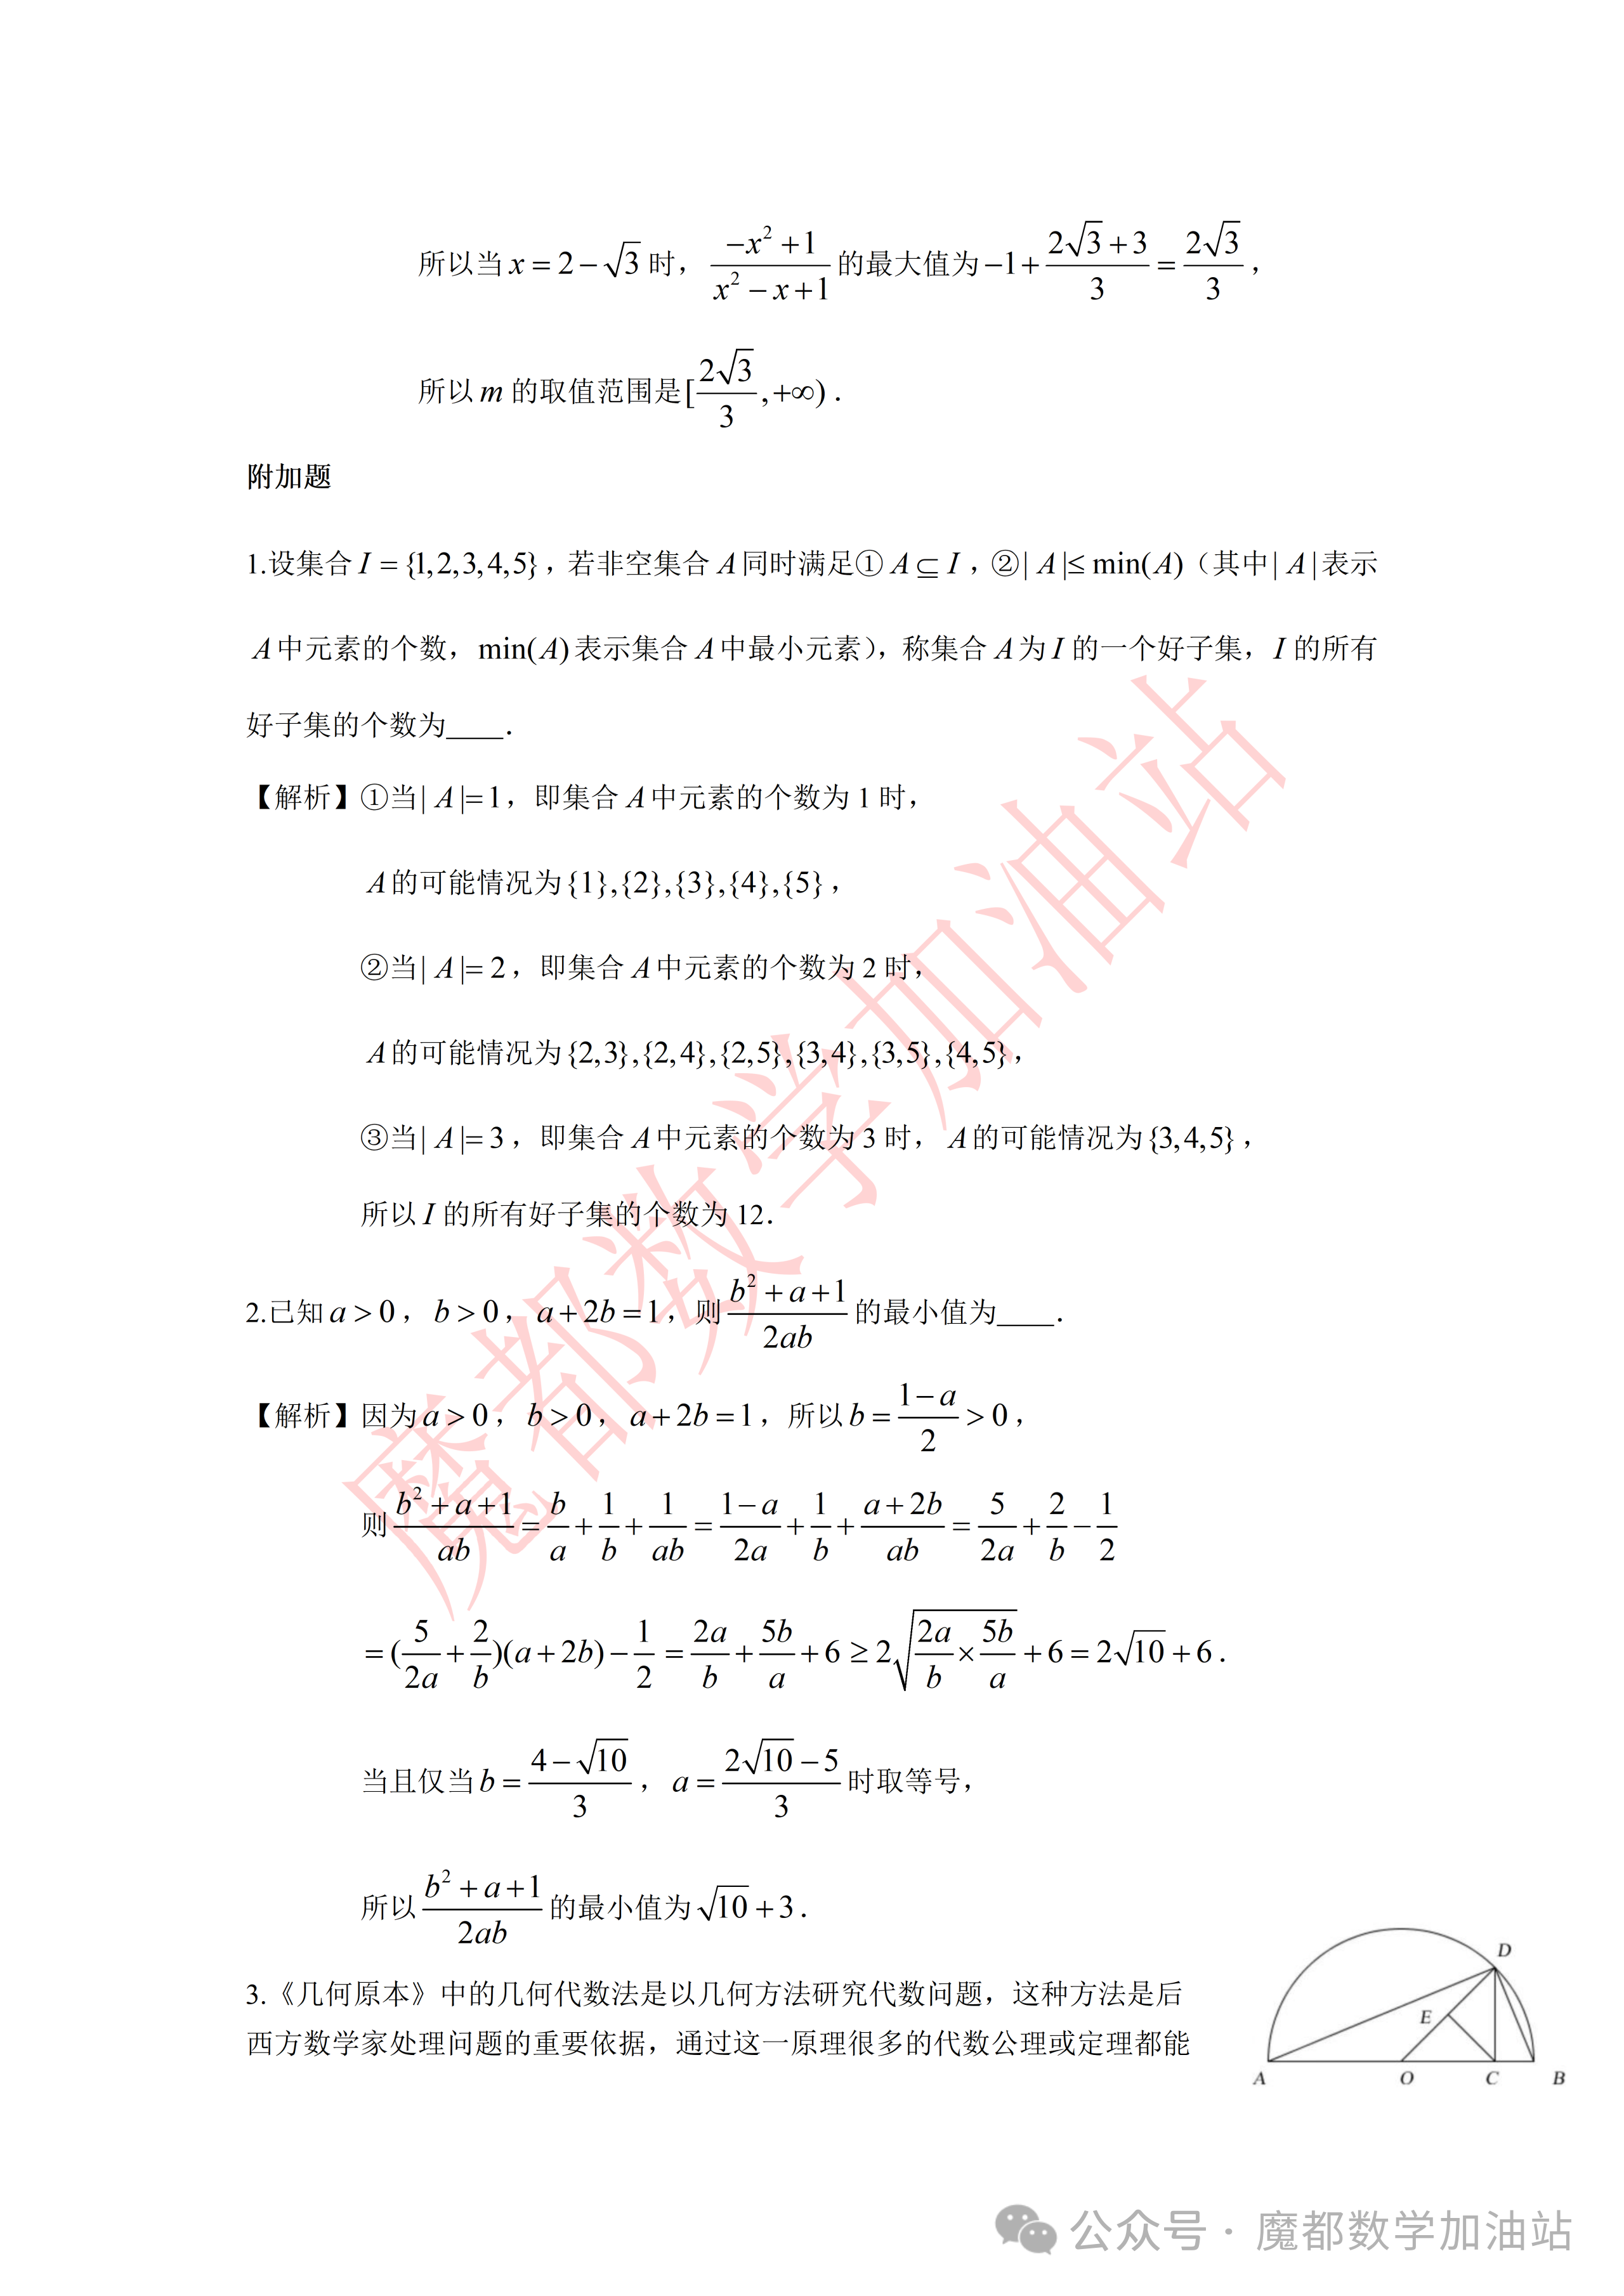
\includegraphics[width=.34\linewidth,trim=1960bp 310bp 90bp 3015bp,clip]{../原图/高一47_七宝中学_抱孩子练习9.26/08.png}
\end{center}

① $\dfrac{a+b}{2}\geqslant\sqrt{ab}$（$a>0$，$b>0$）；
② $a^2+b^2\geqslant2ab$（$a>0$，$b>0$）；
③ $\sqrt{ab}\geqslant\dfrac{2}{\dfrac1a+\dfrac1b}$（$a>0$，$b>0$）；
④ $\sqrt{\dfrac{a^2+b^2}{2}}\geqslant\dfrac{a+b}{2}$（$a>0$，$b>0$）.

\ifanswer
\solbegin
\step{因为 $AC+CB=a+b$，所以 $OD=\dfrac{AB}{2}=\dfrac{AC+CB}{2}=\dfrac{a+b}{2}$；}
\step{由射影定理得 $CD=\sqrt{AC\times CB}=\sqrt{ab}$，又因为 $OD\geqslant CD$，}
\step{所以 $\dfrac{a+b}{2}\geqslant\sqrt{ab}$，故①正确；}
\step{由射影定理得 $CD^2=DE\times OD$，所以 $DE=\dfrac{CD^2}{OD}=\dfrac{ab}{\dfrac{a+b}{2}}=\dfrac{2}{\dfrac1a+\dfrac1b}$，}
\step{又因为 $CD\geqslant DE$，所以 $\sqrt{ab}\geqslant\dfrac{2}{\dfrac1a+\dfrac1b}$，故③正确；}
\step{故该图形可以完成的所有无字证明为①③.}
\solend

\fi

% 注：原卷此处印作等式 $|x^2+a|+|x-a|=|x^2+x|$（在 $x>0$ 时与三角不等式下界等价），本稿曾改写成
% 不等式，现按原卷照录（原卷如此，照录未改）。
\item 若对任意 $x\in[2,3]$，均有 $|x^2+a|+|x-a|=|x^2+x|$，则实数 $a$ 的取值范围为 \blankline[4.4em].

\ifanswer
\solbegin
\step{因为 $|a|+|b|=|a+b|$ 当且仅当 $ab\geqslant0$ 时取等号，}
\step{所以 $(x^2+a)(x-a)\geqslant0$，即 $(a+x^2)(a-x)\leqslant0$，所以 $-x^2\leqslant a\leqslant x$ 恒成立，}
\step{因为 $x\in[2,3]$，所以 $-4\leqslant a\leqslant2$，所以实数 $a$ 的取值范围为 $[-4,2]$.}
\solend

\fi

\end{enumerate}

\end{document}
"
%
% 原始材料是微信公众号图文（公众号“魔都数学加油站”连载“27学年高一47”，署名“破晓”，
% 2026-10-02 17:56 发布，原文标题“27学年高一47——2026-2027年上海市七宝中学高一上抱孩子练习9.26”，
% 原文链接 https://mp.weixin.qq.com/s/mhkyDwjn7QFP_Z_NOcPkQA），正文为 9 张 PNG 页。
% 第 1—7、9 页分辨率为 4762×6735，第 8 页为 2560×3620；均按原图逐页核对。
% 原卷文字、选项、答案与解析均照录；粉色斜水印及灰色公众号页脚属水印/页脚，未录入。
%
% 卷首标题：原卷印作“2026-2027 年七宝中学高一上抱孩子练习 9.26”（公众号标题里的“上海市”
% 三字卷面标题行没有，本稿照卷面），年份区间按全稿惯例排 en dash，作业名保留原卷日期“9.26”。
% 原卷未印独立副标题；本稿按“知识模块”口径补出“集合与常用逻辑用语、不等式”。
%
% 与原卷的排版差异：
%   ① 原卷分“一、填空题”“二、选择题”“三、解答题”“附加题”四节；前三节题号为 3—16，
%      分别有 8 道填空、3 道选择、3 道解答；附加题另起 1—4 编号；
%   ② 原卷题下直接印答案/解析，本稿按全稿统一收进答案版；填空横线采用统一长度；
%   ③ 原卷未印副标题，本稿按“知识模块”口径补出（见卷首标题）；
%   ④ 全卷只有附加题第 3 题带图，直接从原卷第 8 页裁取。
%
% 原卷存疑（照录未改，见源码中该处上方注释）：
%   ① 第 9 题集合 C 的条件原文作“C={x|y=..., x 是整数}”，其中 y 未在集合描述中定义；
%      本稿照录原记号，未代换为 x。
%   ② 附加题第 3 题原文作“后西方数学家”，措辞存疑（疑漏“世”字）；本稿照录未改。
%
\documentclass[a4paper,11pt]{article}
\usepackage{common}

\begin{document}

\examtitlest[3]{2026--2027 年七宝中学高一上抱孩子练习 9.26}{集合与常用逻辑用语、不等式}

\bigsec{一、填空题}

\begin{enumerate}
\setcounter{enumi}{2}

\item 若不等式 $|x|<a$ 的一个充分条件为 $0<x<1$，则实数 $a$ 的取值范围是 \blankline[4.4em].

\ifanswer
\solbegin
\step{由 $|x|<a$ 得到 $-a<x<a$，}
\step{又不等式 $|x|<a$ 的一个充分条件为 $0<x<1$，所以 $a\geqslant1$.}
\solend

\fi

\item 已知命题“$\exists x\in\R$，使 $4x^2+(a-2)x+\dfrac14=0$”是假命题，则实数 $a$ 的取值范围是 \blankline[4.4em].

\ifanswer
\solbegin
% 注：原卷首句作“为真命题”（先按命题为真推出 $\Delta\geqslant0$，再由其为假得 $0<a<4$），原卷如此，照录未改。
\step{命题 $\exists x\in\R$，使 $4x^2+(a-2)x+\dfrac14=0$ 为真命题，}
\step{则 $\Delta=(a-2)^2-4\times4\times\dfrac14=a^2-4a\geqslant0$，解得 $a\leqslant0$ 或 $a\geqslant4$，}
\step{而命题“$\exists x\in\R$，使 $4x^2+(a-2)x+\dfrac14=0$”是假命题，则 $0<a<4$，}
\step{所以实数 $a$ 的取值范围是 $\{a\mid0<a<4\}$.}
\solend

\fi

\item 已知集合 $A=\{x\mid(a-1)x^2+3x-2=0\}$ 有且仅有两个子集，则实数 $a=$ \blankline[4.4em].

\ifanswer
\solbegin
\step{集合 $A=\{x\mid(a-1)x^2+3x-2=0\}$ 有且仅有两个不同的子集，}
\step{所以 $a-1=0$ 或 $\begin{cases}a-1\neq0\\\Delta=9+8(a-1)=0\end{cases}$，解得实数 $a=1$ 或 $a=-\dfrac18$.}
\solend

\fi

\item 已知函数 $y=x^2+bx+3$（其中 $b$ 是实数）中，$y$ 的取值范围是 $[0,+\infty)$，若关于 $x$ 的不等式 $x^2+bx+3<c$ 的解集为 $m-8<x<m$，则实数 $c$ 的值为 \blankline[4.4em].

\ifanswer
\solbegin
\step{因为 $y$ 的取值范围是 $[0,+\infty)$，所以 $\Delta=b^2-12=0$，解得 $b^2=12$，}
\step{因为不等式 $x^2+bx+3<c$ 的解集为 $m-8<x<m$，}
\step{令 $x^2+bx+3=c$，即 $x^2+bx+3-c=0$，方程的两根为 $x_1=m-8$，$x_2=m$，}
\step{所以 $|x_2-x_1|=\sqrt{(x_1+x_2)^2-4x_1x_2}=\sqrt{b^2-4(3-c)}=8$，即 $\sqrt{12-4(3-c)}=8$，}
\step{且判别式 $\Delta=b^2-4(3-c)=12-4(3-c)>0$，解得 $c=16$.}
\solend

\fi

\item 关于 $x$ 的不等式 $|x-1|+|x+1|\geqslant a$ 的解集为 $\R$，则实数 $a$ 的取值范围为 \blankline[4.4em].

\ifanswer
\solbegin
\step{因为 $|x-1|+|x+1|\geqslant|x-1-(x+1)|=2$，}
\step{若关于 $x$ 的不等式 $|x-1|+|x+1|\geqslant a$ 的解集为 $\R$，则实数 $a$ 的取值范围为 $a\leqslant2$.}
\solend

\fi

\item 已知 $m>0$，$xy>0$，当 $x+y=2$ 时，不等式 $\dfrac2x+\dfrac my\geqslant4$ 恒成立，则 $m$ 的取值范围是 \blankline[4.4em].

\ifanswer
\solbegin
\step{因为 $m>0$，$xy>0$，$x+y=2$，}
\step{所以 $\dfrac2x+\dfrac my=\dfrac12(x+y)\left(\dfrac2x+\dfrac my\right)
=\dfrac12\left(m+2+\dfrac{2y}{x}+\dfrac{mx}{y}\right)$}
\step{$\geqslant\dfrac12\left(m+2+2\sqrt{\dfrac{2y}{x}\cdot\dfrac{mx}{y}}\right)=\dfrac12\left(m+2+2\sqrt{2m}\right)$，}
\step{当且仅当 $\dfrac{2y}{x}=\dfrac{mx}{y}$，即 $y^2=\dfrac{mx^2}{2}$ 时取等号.}
\step{因为不等式 $\dfrac2x+\dfrac my\geqslant4$ 恒成立，所以 $\dfrac12(m+2+2\sqrt{2m})\geqslant4$，}
\step{整理得 $(\sqrt m+3\sqrt2)(\sqrt m-\sqrt2)\geqslant0$，解得 $\sqrt m\geqslant\sqrt2$，即 $m\geqslant2$，}
\step{所以 $m$ 的取值范围为 $[2,+\infty)$.}
\solend

\fi

\item 已知全集为 $\R$，集合 $D=\{x\mid x^2-ax+a^2-19=0\}$，
$B=\{y\mid y=-x^2+2x+2,\ y\text{ 是正整数}\}$，
% 注：本题集合 C 的条件原文作“C={x|y=..., x 是整数}”，其中 y 未在集合描述中定义；照录未改。
集合 $C=\left\{x\mathrel{\Big|}y=\sqrt{\dfrac{2-x}{x+1}},\ x\text{ 是整数}\right\}$，且集合 $D$ 满足 $D\cap B\neq\varnothing$，$\overline{D}\cup\overline{C}=\R$，则实数 $a$ 的值是 \blankline[4.4em].

\ifanswer
\solbegin
\step{集合 $B=\{y\mid y=-x^2+2x+2,\ y\text{ 是正整数}\}=\{1,2,3\}$，}
\step{集合 $C=\left\{x\mathrel{\Big|}y=\sqrt{\dfrac{2-x}{x+1}},\ x\text{ 是整数}\right\}=\{0,1,2\}$，}
\step{集合 $D=\{x\mid x^2-ax+a^2-19=0\}$ 且集合 $D$ 满足 $D\cap B\neq\varnothing$，$\overline{D}\cup\overline{C}=\R$，}
\step{所以 $3\in D$，解得 $a=5$ 或 $a=-2$，}
\step{经检验，$a=5$ 不符合 $\overline{D}\cup\overline{C}=\R$，舍去，$a=-2$ 满足题意，即 $a=-2$.}
\solend

\fi

% 注：本题解析中，$a=\pm2\sqrt2$ 时 $B$ 的二重根按 $-\dfrac a2$ 应为 $\mp\sqrt2$，原卷印作 $\mp2\sqrt2$、
% $-\dfrac{3\sqrt2}4$，$C(B)=3$ 的计算也随之按原卷保留（原卷如此，照录未改）。
\item 用 $C(A)$ 表示非空集合 $A$ 中的元素的个数，定义 $A*B=|C(A)-C(B)|$，已知集合 $A$ 有三个真子集，
$B=\{x\mid(ax^2+3x)(x^2+ax+2)=0,\ x\in\R\}$，若 $A*B=1$，设实数 $a$ 所有可能取值构成集合 $S$，则 $C(S)=$ \blankline[4.4em].

\ifanswer
\solbegin
\step{集合 $A$ 有三个真子集，则集合 $A$ 中有 $2$ 个元素，则 $C(A)=2$，}
\step{由 $A*B=1$，得 $C(B)=1$ 或 $3$，}
\step{即方程 $(ax^2+3x)\cdot(x^2+ax+2)=0$ 有一个根或 $3$ 个根；}
\step{若 $(ax^2+3x)\cdot(x^2+ax+2)=0$，则必有 $ax^2+3x=0$ 或 $x^2+ax+2=0$，}
\step{若 $ax^2+3x=0$，则 $x=0$ 或 $ax+3=0$，}
\step{当 $a=0$ 时，$B=\{0\}$，$C(B)=1$，符合题意；}
\step{当 $a\neq0$ 时，$ax^2+3x=0$ 对应的根为 $0$ 和 $-\dfrac3a$；}
\step{故①需 $x^2+ax+2=0$ 有两等根且根不为 $0$ 和 $-\dfrac3a$，}
\step{当 $\Delta=0$ 时，$a=\pm2\sqrt2$，}
\step{$a=2\sqrt2$，此时 $B=\left\{0,-2\sqrt2,-\dfrac{3\sqrt2}{4}\right\}$，$C(B)=3$，符合题意；}
\step{$a=-2\sqrt2$，此时 $B=\left\{0,2\sqrt2,\dfrac{3\sqrt2}{4}\right\}$，$C(B)=3$，符合题意；}
\step{②当 $-\dfrac3a$ 是 $x^2+ax+2=0$ 的根时，解得 $a=\pm3$；}
\step{$a=3$，此时 $B=\{0,-1,-2\}$，$C(B)=3$，符合题意；}
\step{$a=-3$，此时 $B=\{0,1,2\}$，$C(B)=3$，符合题意；}
\step{综上，$a$ 可取的值为 $0$、$\pm3$、$\pm2\sqrt2$，则 $C(S)=5$.}
\solend

\fi

\end{enumerate}

\bigsec{二、选择题}

\begin{enumerate}
\setcounter{enumi}{10}

\item 已知集合 $A=\left\{x\mathrel{\Big|}\dfrac1x<1\right\}$，$B=\{x\mid x^2-2x-3\leqslant0\}$，则 $A\cap B=$\mbox{（\quad）}

\keepwithprev
A. $\{x\mid1<x\leqslant3\}$\qquad B. $\{x\mid1\leqslant x\leqslant3\text{ 或 }-1\leqslant x<0\}$

C. $\{x\mid-1\leqslant x<0\}$\qquad D. $\{x\mid1<x\leqslant3\text{ 或 }-1\leqslant x<0\}$

\ans{$D$}

% 注：原卷本题只有题干＋选项（答案印在括号内），没有解析；此处照录原卷的"无解析"状态，不排解析。
\item 使 $x(y-2)=0$ 成立的一个充分条件是\mbox{（\quad）}

\keepwithprev
A. $x^2+(y-2)^2=0$\qquad B. $(x-2)^2+y^2=0$

C. $x^2+y^2=1$\qquad D. $x+y-2=0$

\ans{$A$}

\ifanswer
\solbegin
\step{对于 $A$：若 $x^2+(y-2)^2=0$，则 $x=0$ 且 $y=2$，此时 $x(y-2)=0$ 成立，}
\step{即充分性成立.}
\step{若 $x(y-2)=0$，则 $x=0$ 或 $y=2$，当 $x=0$，$y=3$ 时，$x^2+(y-2)^2=0$ 不成立，}
\step{即必要性不成立，}
\step{故 $x^2+(y-2)^2=0$ 是 $x(y-2)=0$ 成立的充分不必要条件；}
\step{对于 $B$：$(x-2)^2+y^2=0$，则 $x=2$ 且 $y=0$，此时 $x(y-2)=0$ 不成立，}
\step{即充分性不成立；}
\step{对于 $C$：$x^2+y^2=1$，此时 $x(y-2)=0$ 不一定成立，即充分性不成立；}
\step{对于 $D$：$x+y-2=0$，此时 $x(y-2)=0$ 不一定成立，即充分性不成立.}
\step{故选 $A$.}
\solend

\fi

\item 已知 $a$、$b$、$c\in\R$，若关于 $x$ 的不等式 $0\leqslant x+\dfrac ax+b\leqslant\dfrac cx-1$ 的解集为 $[x_1,x_2]\cup\{x_3\}$（$x_3>x_2>x_1>0$），则\mbox{（\quad）}

\keepwithprev
A. 不存在有序数组 $(a,b,c)$，使得 $x_2-x_1=1$

B. 存在唯一有序数组 $(a,b,c)$，使得 $x_2-x_1=1$

C. 有且只有两组有序数组 $(a,b,c)$，使得 $x_2-x_1=1$

D. 存在无穷多组有序数组 $(a,b,c)$，使得 $x_2-x_1=1$

\ans{$D$}

\ifanswer
\solbegin
\step{因为不等式 $0\leqslant x+\dfrac ax+b\leqslant\dfrac cx-1$ 的解集为 $[x_1,x_2]\cup\{x_3\}$（$x_3>x_2>x_1>0$），}
\step{所以 $0\leqslant x^2+bx+a\leqslant c-x$ 在 $[x_1,x_2]\cup\{x_3\}$ 上成立，}
\step{假设 $x_1=m$，$x_2=m+1$，$x_3=n$，}
\step{则 $c-n=0=n^2+bn+a$，由 $x_3$ 为一个独立的数得出，}
\step{所以 $n=c$，且 $m+1$ 与 $n$ 为方程 $x^2+bx+a=0$ 的两个根，}
\step{因为 $x_3>x_2>x_1>0$，所以 $-b=m+n+1=m+c+1$，$a=mn+n=mc+c$，}
\step{所以 $b=-m-c-1$，}
\step{且点 $(x_1,x_1^2+bx_1+a)$ 为 $y=x^2+bx+a$ 与 $y=c-x$ 的左交点，}
\step{所以 $m^2+bm+a=c-m$ 且 $b=-m-c-1$，$a=mc+c$，}
% 注：原卷此行的末句作“所以 $c-m=c-m$ 恒成立”（未写成 $x_2-x_1=1$），原卷如此，照录未改。
\step{故 $m^2+bm+a=m^2-m^2-mc-m+mc+c=c-m$，所以 $c-m=c-m$ 恒成立，}
\step{所以不论 $a$、$b$、$c$ 取何值，$x_2-x_1=1$ 恒成立，}
\step{即存在无穷多组有序数组 $(a,b,c)$，使得 $x_2-x_1=1$，}
\step{故选项 $A$、$B$、$C$ 错误，选项 $D$ 正确. 故选 $D$.}
\solend

\fi

\end{enumerate}

\bigsec{三、解答题}

\begin{enumerate}
\setcounter{enumi}{13}

\item 设正实数 $x$、$y$，满足 $2x+y=1$，求：

\begin{enumerate}[label=(\arabic*)]
\item $\sqrt{2x}+\sqrt y$ 的最大值；
\item $\dfrac2x+\dfrac1y$ 的最小值.
\end{enumerate}

\ifanswer
\solbegin
\stepm{(1)}{对于 $(\sqrt{2x}+\sqrt y)^2=2x+y+2\sqrt{2xy}\leqslant1+1=2$，}
\step{当且仅当 $\sqrt{2x}=\sqrt y$ 时取等号，故 $\sqrt{2x}+\sqrt y$ 的最大值为 $\sqrt2$；}
\stepm{(2)}{$\dfrac2x+\dfrac1y=\left(\dfrac2x+\dfrac1y\right)(2x+y)=5+\dfrac{2y}{x}+\dfrac{2x}{y}\geqslant5+4=9$，}
\step{当且仅当 $\dfrac{2y}{x}=\dfrac{2x}{y}$，即 $x=y=\dfrac13$ 时取等号，故 $\dfrac2x+\dfrac1y$ 的最小值为 $9$.}
\solend

\fi

\ansspace[6]

\item 设 $x_1$、$x_2$ 为关于 $x$ 的方程 $x^2-2(m+2)x+m^2-1=0$ 的两实数根.

\begin{enumerate}[label=(\arabic*)]
\item 若 $x_1$、$x_2$ 满足 $x_1^2+x_2^2=18$，试求 $m$ 的值；
\item 若 $x_1$、$x_2$ 均大于 $0$，求 $m$ 的取值范围.
\end{enumerate}

\ifanswer
\solbegin
\stepm{(1)}{由 $\Delta=4(m+2)^2-4(m^2-1)\geqslant0$，解得 $m\geqslant-\dfrac54$，}
\step{由韦达定理得 $x_1+x_2=2(m+2)$，$x_1x_2=m^2-1$，}
\step{又 $x_1^2+x_2^2=(x_1+x_2)^2-2x_1x_2=4(m+2)^2-2(m^2-1)=18$，}
\step{即 $m^2+8m=0$，解得 $m=0$ 或 $m=-8$（舍），故 $m$ 的值为 $0$；}
% 注：原卷此处作“由（2）得”（对照上一小问，所指应为（1）），原卷如此，照录未改。
\stepm{(2)}{由（2）得 $m\geqslant-\dfrac54$，}
\step{又 $x_1$、$x_2$ 均大于 $0$，则 $\begin{cases}2(m+2)>0\\m^2-1>0\end{cases}$，解得 $\begin{cases}m>-2\\m>1\text{或}m<-1\end{cases}$，}
\step{综上，实数 $m$ 的取值范围为 $\left[-\dfrac54,-1\right)\cup(1,+\infty)$.}
\solend

\fi

\ansspace[6]

\item 已知函数 $f(x)=(m+1)x^2-mx+m-1$（$m\in\R$）.

\begin{enumerate}[label=(\arabic*)]
\item 若不等式 $f(x)<0$ 的解集是空集，求 $m$ 的取值范围；
\item 当 $m>-2$ 时，解不等式 $f(x)\geqslant m$；
\item 若不等式 $f(x)\geqslant0$ 的解集为 $D$，若 $[-1,1]\subseteq D$，求 $m$ 的取值范围.
\end{enumerate}

\ifanswer
\solbegin
\stepm{(1)}{①当 $m+1=0$，即 $m=-1$ 时，$f(x)=x-2$，不合题意；}
\step{②当 $m+1\neq0$，即 $m\neq-1$ 时，$\begin{cases}m+1>0\\\Delta=m^2-4(m+1)(m-1)\leqslant0\end{cases}$，解得 $m\geqslant\dfrac{2\sqrt3}{3}$，}
\step{所以 $m$ 的取值范围是 $\left[\dfrac{2\sqrt3}{3},+\infty\right)$；}
\stepm{(2)}{因为 $f(x)\geqslant m$，所以 $(m+1)x^2-mx-1\geqslant0$，即 $[(m+1)x+1](x-1)\geqslant0$，}
\step{①当 $m+1=0$ 即 $m=-1$ 时，不等式的解集为 $[1,+\infty)$；}
\step{②当 $m+1>0$ 即 $m>-1$ 时，$\left(x+\dfrac1{m+1}\right)(x-1)\geqslant0$，}
\step{因为 $-\dfrac1{m+1}<0$，所以不等式的解集为 $\left(-\infty,-\dfrac1{m+1}\right]\cup[1,+\infty)$；}
\step{③当 $m+1<0$ 即 $-2<m<-1$ 时，$\left(x+\dfrac1{m+1}\right)(x-1)\leqslant0$，}
\step{因为 $-2<m<-1$，所以 $-1<m+1<0$，所以 $-\dfrac1{m+1}>1$，}
\step{所以不等式的解集为 $\left[1,-\dfrac1{m+1}\right]$；}
\stepm{(3)}{不等式 $f(x)\geqslant0$ 的解集为 $D$，若 $[-1,1]\subseteq D$，}
\step{即对任意的 $x\in[-1,1]$，不等式 $(m+1)x^2-mx+m-1\geqslant0$ 恒成立，}
\step{即 $m(x^2-x+1)\geqslant-x^2+1$ 恒成立，}
\step{因为 $x^2-x+1>0$ 恒成立，所以 $m\geqslant\dfrac{-x^2+1}{x^2-x+1}=-1+\dfrac{2-x}{x^2-x+1}$ 恒成立，}
\step{设 $t=2-x$，则 $t\in[1,3]$，$x=2-t$，}
\step{则 $\dfrac{2-x}{x^2-x+1}=\dfrac{t}{(2-t)^2-(2-t)+1}=\dfrac{t}{t^2-3t+3}=\dfrac1{t+\dfrac3t-3}$，}
\step{因为 $t+\dfrac3t\geqslant2\sqrt3$，当且仅当 $t=\sqrt3$ 时取等号，}
\step{所以 $\dfrac{2-x}{x^2-x+1}\leqslant\dfrac1{2\sqrt3-3}=\dfrac{2\sqrt3+3}{3}$，当且仅当 $x=2-\sqrt3$ 时取等号，}
\step{所以当 $x=2-\sqrt3$ 时，$\dfrac{-x^2+1}{x^2-x+1}$ 的最大值为 $-1+\dfrac{2\sqrt3+3}{3}=\dfrac{2\sqrt3}{3}$，}
\step{所以 $m$ 的取值范围是 $\left[\dfrac{2\sqrt3}{3},+\infty\right)$.}
\solend

\fi

\ansspace[8]

\end{enumerate}

\bigsec{附加题}

\begin{enumerate}

\item 设集合 $I=\{1,2,3,4,5\}$，若非空集合 $A$ 同时满足① $A\subseteq I$，② $|A|\leqslant\min(A)$（其中 $|A|$ 表示集合 $A$ 中元素的个数，$\min(A)$ 表示集合 $A$ 中最小元素），称集合 $A$ 为 $I$ 的一个好子集，$I$ 所有好子集的个数为 \blankline[4.4em].

\ifanswer
\solbegin
\step{①当 $|A|=1$，即集合 $A$ 中元素的个数为 $1$ 时，}
\step{$A$ 的可能情况为 $\{1\}$、$\{2\}$、$\{3\}$、$\{4\}$、$\{5\}$，}
\step{②当 $|A|=2$，即集合 $A$ 中元素的个数为 $2$ 时，}
\step{$A$ 的可能情况为 $\{2,3\}$、$\{2,4\}$、$\{2,5\}$、$\{3,4\}$、$\{3,5\}$、$\{4,5\}$，}
\step{③当 $|A|=3$，即集合 $A$ 中元素的个数为 $3$ 时，$A$ 的可能情况为 $\{3,4,5\}$，}
\step{所以 $I$ 的所有好子集的个数为 $12$.}
\solend

\fi

\item 已知 $a>0$，$b>0$，$a+2b=1$，则 $\dfrac{b^2+a+1}{2ab}$ 的最小值为 \blankline[4.4em].

\ifanswer
\solbegin
\step{因为 $a>0$，$b>0$，$a+2b=1$，所以 $b=\dfrac{1-a}{2}>0$，}
\step{则 $\dfrac{b^2+a+1}{ab}=\dfrac ba+\dfrac1b+\dfrac1{ab}=\dfrac{1-a}{2a}+\dfrac1b+\dfrac{a+2b}{ab}=\dfrac5{2a}+\dfrac2b-\dfrac12$}
\step{$=\left(\dfrac5{2a}+\dfrac2b\right)(a+2b)-\dfrac12=\dfrac{2a}{b}+\dfrac{5b}{a}+6\geqslant2\sqrt{\dfrac{2a}{b}\times\dfrac{5b}{a}}+6=2\sqrt{10}+6$.}
\step{当且仅当 $b=\dfrac{4-\sqrt{10}}{3}$，$a=\dfrac{2\sqrt{10}-5}{3}$ 时取等号，}
\step{所以 $\dfrac{b^2+a+1}{2ab}$ 的最小值为 $\sqrt{10}+3$.}
\solend

\fi

% 注：本题原文作“后西方数学家”，措辞存疑（疑漏“世”字）；照录未改，见文件头“原卷存疑”②。
% 又原文作"很多的代数公理或定理都能够通过图形实现证明"（"公理"疑为"公式"笔误）、
% "连结 OD,AD,BD"，均原卷如此，照录未改。
\item 《几何原本》中的几何代数法是以几何方法研究代数问题，这种方法是后西方数学家处理问题的重要依据，通过这一原理很多的代数公理或定理都能够通过图形实现证明，也称之为无字证明，现有图形如图所示，$C$ 为线段 $AB$ 上的点，且 $AC=a$，$BC=b$，$O$ 为 $AB$ 的中点，以 $AB$ 为直径作半圆，过点 $C$ 作 $AB$ 的垂线交半圆于 $D$，连结 $OD,AD,BD$，过点 $C$ 作 $OD$ 的垂线，垂足为 $E$，若不添加辅助线，则该图形可以完成的所有无字证明为 \blankline[4.4em]（填写序号）.

\begin{center}
% 插图直接裁自原卷第 8 页，未重绘；用 trim/clip 保留原图与标注。
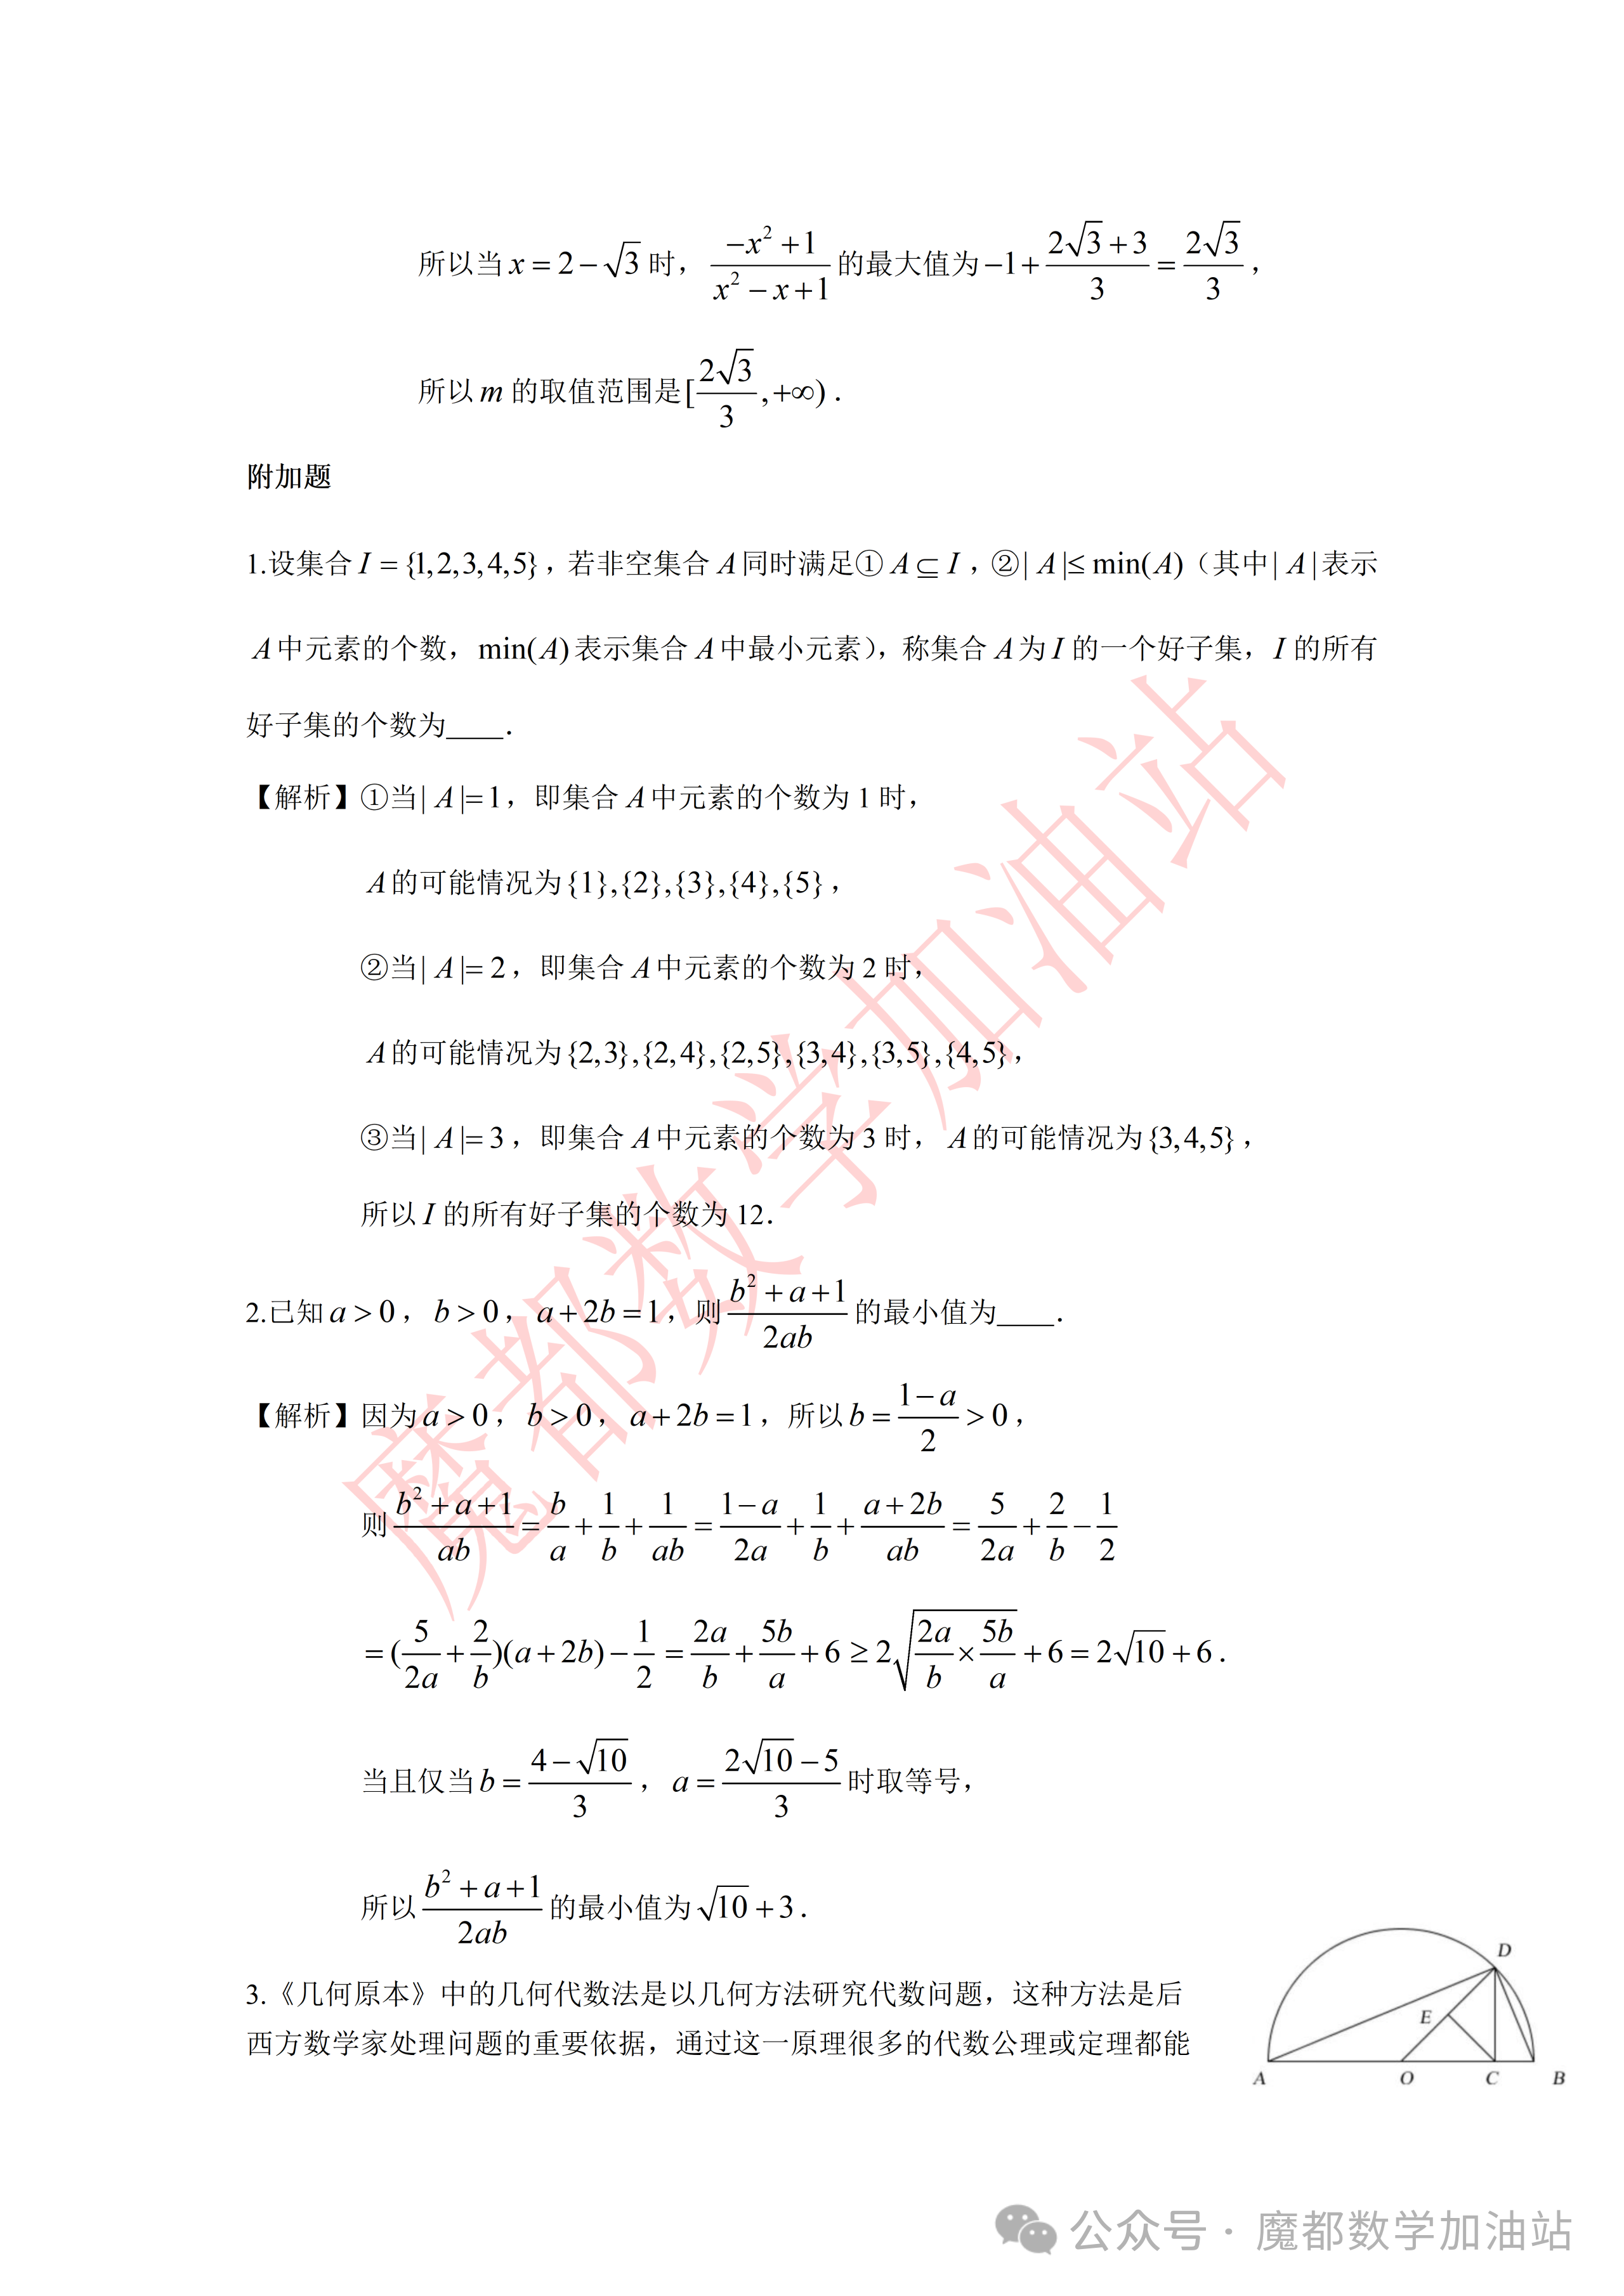
\includegraphics[width=.34\linewidth,trim=1960bp 310bp 90bp 3015bp,clip]{../原图/高一47_七宝中学_抱孩子练习9.26/08.png}
\end{center}

① $\dfrac{a+b}{2}\geqslant\sqrt{ab}$（$a>0$，$b>0$）；
② $a^2+b^2\geqslant2ab$（$a>0$，$b>0$）；
③ $\sqrt{ab}\geqslant\dfrac{2}{\dfrac1a+\dfrac1b}$（$a>0$，$b>0$）；
④ $\sqrt{\dfrac{a^2+b^2}{2}}\geqslant\dfrac{a+b}{2}$（$a>0$，$b>0$）.

\ifanswer
\solbegin
\step{因为 $AC+CB=a+b$，所以 $OD=\dfrac{AB}{2}=\dfrac{AC+CB}{2}=\dfrac{a+b}{2}$；}
\step{由射影定理得 $CD=\sqrt{AC\times CB}=\sqrt{ab}$，又因为 $OD\geqslant CD$，}
\step{所以 $\dfrac{a+b}{2}\geqslant\sqrt{ab}$，故①正确；}
\step{由射影定理得 $CD^2=DE\times OD$，所以 $DE=\dfrac{CD^2}{OD}=\dfrac{ab}{\dfrac{a+b}{2}}=\dfrac{2}{\dfrac1a+\dfrac1b}$，}
\step{又因为 $CD\geqslant DE$，所以 $\sqrt{ab}\geqslant\dfrac{2}{\dfrac1a+\dfrac1b}$，故③正确；}
\step{故该图形可以完成的所有无字证明为①③.}
\solend

\fi

% 注：原卷此处印作等式 $|x^2+a|+|x-a|=|x^2+x|$（在 $x>0$ 时与三角不等式下界等价），本稿曾改写成
% 不等式，现按原卷照录（原卷如此，照录未改）。
\item 若对任意 $x\in[2,3]$，均有 $|x^2+a|+|x-a|=|x^2+x|$，则实数 $a$ 的取值范围为 \blankline[4.4em].

\ifanswer
\solbegin
\step{因为 $|a|+|b|=|a+b|$ 当且仅当 $ab\geqslant0$ 时取等号，}
\step{所以 $(x^2+a)(x-a)\geqslant0$，即 $(a+x^2)(a-x)\leqslant0$，所以 $-x^2\leqslant a\leqslant x$ 恒成立，}
\step{因为 $x\in[2,3]$，所以 $-4\leqslant a\leqslant2$，所以实数 $a$ 的取值范围为 $[-4,2]$.}
\solend

\fi

\end{enumerate}

\end{document}
"
%
% 原始材料是微信公众号图文（公众号“魔都数学加油站”连载“27学年高一47”，署名“破晓”，
% 2026-10-02 17:56 发布，原文标题“27学年高一47——2026-2027年上海市七宝中学高一上抱孩子练习9.26”，
% 原文链接 https://mp.weixin.qq.com/s/mhkyDwjn7QFP_Z_NOcPkQA），正文为 9 张 PNG 页。
% 第 1—7、9 页分辨率为 4762×6735，第 8 页为 2560×3620；均按原图逐页核对。
% 原卷文字、选项、答案与解析均照录；粉色斜水印及灰色公众号页脚属水印/页脚，未录入。
%
% 卷首标题：原卷印作“2026-2027 年七宝中学高一上抱孩子练习 9.26”（公众号标题里的“上海市”
% 三字卷面标题行没有，本稿照卷面），年份区间按全稿惯例排 en dash，作业名保留原卷日期“9.26”。
% 原卷未印独立副标题；本稿按“知识模块”口径补出“集合与常用逻辑用语、不等式”。
%
% 与原卷的排版差异：
%   ① 原卷分“一、填空题”“二、选择题”“三、解答题”“附加题”四节；前三节题号为 3—16，
%      分别有 8 道填空、3 道选择、3 道解答；附加题另起 1—4 编号；
%   ② 原卷题下直接印答案/解析，本稿按全稿统一收进答案版；填空横线采用统一长度；
%   ③ 原卷未印副标题，本稿按“知识模块”口径补出（见卷首标题）；
%   ④ 全卷只有附加题第 3 题带图，直接从原卷第 8 页裁取。
%
% 原卷存疑（照录未改，见源码中该处上方注释）：
%   ① 第 9 题集合 C 的条件原文作“C={x|y=..., x 是整数}”，其中 y 未在集合描述中定义；
%      本稿照录原记号，未代换为 x。
%   ② 附加题第 3 题原文作“后西方数学家”，措辞存疑（疑漏“世”字）；本稿照录未改。
%
\documentclass[a4paper,11pt]{article}
\usepackage{common}

\begin{document}

\examtitlest[3]{2026--2027 年七宝中学高一上抱孩子练习 9.26}{集合与常用逻辑用语、不等式}

\bigsec{一、填空题}

\begin{enumerate}
\setcounter{enumi}{2}

\item 若不等式 $|x|<a$ 的一个充分条件为 $0<x<1$，则实数 $a$ 的取值范围是 \blankline[4.4em].

\ifanswer
\solbegin
\step{由 $|x|<a$ 得到 $-a<x<a$，}
\step{又不等式 $|x|<a$ 的一个充分条件为 $0<x<1$，所以 $a\geqslant1$.}
\solend

\fi

\item 已知命题“$\exists x\in\R$，使 $4x^2+(a-2)x+\dfrac14=0$”是假命题，则实数 $a$ 的取值范围是 \blankline[4.4em].

\ifanswer
\solbegin
% 注：原卷首句作“为真命题”（先按命题为真推出 $\Delta\geqslant0$，再由其为假得 $0<a<4$），原卷如此，照录未改。
\step{命题 $\exists x\in\R$，使 $4x^2+(a-2)x+\dfrac14=0$ 为真命题，}
\step{则 $\Delta=(a-2)^2-4\times4\times\dfrac14=a^2-4a\geqslant0$，解得 $a\leqslant0$ 或 $a\geqslant4$，}
\step{而命题“$\exists x\in\R$，使 $4x^2+(a-2)x+\dfrac14=0$”是假命题，则 $0<a<4$，}
\step{所以实数 $a$ 的取值范围是 $\{a\mid0<a<4\}$.}
\solend

\fi

\item 已知集合 $A=\{x\mid(a-1)x^2+3x-2=0\}$ 有且仅有两个子集，则实数 $a=$ \blankline[4.4em].

\ifanswer
\solbegin
\step{集合 $A=\{x\mid(a-1)x^2+3x-2=0\}$ 有且仅有两个不同的子集，}
\step{所以 $a-1=0$ 或 $\begin{cases}a-1\neq0\\\Delta=9+8(a-1)=0\end{cases}$，解得实数 $a=1$ 或 $a=-\dfrac18$.}
\solend

\fi

\item 已知函数 $y=x^2+bx+3$（其中 $b$ 是实数）中，$y$ 的取值范围是 $[0,+\infty)$，若关于 $x$ 的不等式 $x^2+bx+3<c$ 的解集为 $m-8<x<m$，则实数 $c$ 的值为 \blankline[4.4em].

\ifanswer
\solbegin
\step{因为 $y$ 的取值范围是 $[0,+\infty)$，所以 $\Delta=b^2-12=0$，解得 $b^2=12$，}
\step{因为不等式 $x^2+bx+3<c$ 的解集为 $m-8<x<m$，}
\step{令 $x^2+bx+3=c$，即 $x^2+bx+3-c=0$，方程的两根为 $x_1=m-8$，$x_2=m$，}
\step{所以 $|x_2-x_1|=\sqrt{(x_1+x_2)^2-4x_1x_2}=\sqrt{b^2-4(3-c)}=8$，即 $\sqrt{12-4(3-c)}=8$，}
\step{且判别式 $\Delta=b^2-4(3-c)=12-4(3-c)>0$，解得 $c=16$.}
\solend

\fi

\item 关于 $x$ 的不等式 $|x-1|+|x+1|\geqslant a$ 的解集为 $\R$，则实数 $a$ 的取值范围为 \blankline[4.4em].

\ifanswer
\solbegin
\step{因为 $|x-1|+|x+1|\geqslant|x-1-(x+1)|=2$，}
\step{若关于 $x$ 的不等式 $|x-1|+|x+1|\geqslant a$ 的解集为 $\R$，则实数 $a$ 的取值范围为 $a\leqslant2$.}
\solend

\fi

\item 已知 $m>0$，$xy>0$，当 $x+y=2$ 时，不等式 $\dfrac2x+\dfrac my\geqslant4$ 恒成立，则 $m$ 的取值范围是 \blankline[4.4em].

\ifanswer
\solbegin
\step{因为 $m>0$，$xy>0$，$x+y=2$，}
\step{所以 $\dfrac2x+\dfrac my=\dfrac12(x+y)\left(\dfrac2x+\dfrac my\right)
=\dfrac12\left(m+2+\dfrac{2y}{x}+\dfrac{mx}{y}\right)$}
\step{$\geqslant\dfrac12\left(m+2+2\sqrt{\dfrac{2y}{x}\cdot\dfrac{mx}{y}}\right)=\dfrac12\left(m+2+2\sqrt{2m}\right)$，}
\step{当且仅当 $\dfrac{2y}{x}=\dfrac{mx}{y}$，即 $y^2=\dfrac{mx^2}{2}$ 时取等号.}
\step{因为不等式 $\dfrac2x+\dfrac my\geqslant4$ 恒成立，所以 $\dfrac12(m+2+2\sqrt{2m})\geqslant4$，}
\step{整理得 $(\sqrt m+3\sqrt2)(\sqrt m-\sqrt2)\geqslant0$，解得 $\sqrt m\geqslant\sqrt2$，即 $m\geqslant2$，}
\step{所以 $m$ 的取值范围为 $[2,+\infty)$.}
\solend

\fi

\item 已知全集为 $\R$，集合 $D=\{x\mid x^2-ax+a^2-19=0\}$，
$B=\{y\mid y=-x^2+2x+2,\ y\text{ 是正整数}\}$，
% 注：本题集合 C 的条件原文作“C={x|y=..., x 是整数}”，其中 y 未在集合描述中定义；照录未改。
集合 $C=\left\{x\mathrel{\Big|}y=\sqrt{\dfrac{2-x}{x+1}},\ x\text{ 是整数}\right\}$，且集合 $D$ 满足 $D\cap B\neq\varnothing$，$\overline{D}\cup\overline{C}=\R$，则实数 $a$ 的值是 \blankline[4.4em].

\ifanswer
\solbegin
\step{集合 $B=\{y\mid y=-x^2+2x+2,\ y\text{ 是正整数}\}=\{1,2,3\}$，}
\step{集合 $C=\left\{x\mathrel{\Big|}y=\sqrt{\dfrac{2-x}{x+1}},\ x\text{ 是整数}\right\}=\{0,1,2\}$，}
\step{集合 $D=\{x\mid x^2-ax+a^2-19=0\}$ 且集合 $D$ 满足 $D\cap B\neq\varnothing$，$\overline{D}\cup\overline{C}=\R$，}
\step{所以 $3\in D$，解得 $a=5$ 或 $a=-2$，}
\step{经检验，$a=5$ 不符合 $\overline{D}\cup\overline{C}=\R$，舍去，$a=-2$ 满足题意，即 $a=-2$.}
\solend

\fi

% 注：本题解析中，$a=\pm2\sqrt2$ 时 $B$ 的二重根按 $-\dfrac a2$ 应为 $\mp\sqrt2$，原卷印作 $\mp2\sqrt2$、
% $-\dfrac{3\sqrt2}4$，$C(B)=3$ 的计算也随之按原卷保留（原卷如此，照录未改）。
\item 用 $C(A)$ 表示非空集合 $A$ 中的元素的个数，定义 $A*B=|C(A)-C(B)|$，已知集合 $A$ 有三个真子集，
$B=\{x\mid(ax^2+3x)(x^2+ax+2)=0,\ x\in\R\}$，若 $A*B=1$，设实数 $a$ 所有可能取值构成集合 $S$，则 $C(S)=$ \blankline[4.4em].

\ifanswer
\solbegin
\step{集合 $A$ 有三个真子集，则集合 $A$ 中有 $2$ 个元素，则 $C(A)=2$，}
\step{由 $A*B=1$，得 $C(B)=1$ 或 $3$，}
\step{即方程 $(ax^2+3x)\cdot(x^2+ax+2)=0$ 有一个根或 $3$ 个根；}
\step{若 $(ax^2+3x)\cdot(x^2+ax+2)=0$，则必有 $ax^2+3x=0$ 或 $x^2+ax+2=0$，}
\step{若 $ax^2+3x=0$，则 $x=0$ 或 $ax+3=0$，}
\step{当 $a=0$ 时，$B=\{0\}$，$C(B)=1$，符合题意；}
\step{当 $a\neq0$ 时，$ax^2+3x=0$ 对应的根为 $0$ 和 $-\dfrac3a$；}
\step{故①需 $x^2+ax+2=0$ 有两等根且根不为 $0$ 和 $-\dfrac3a$，}
\step{当 $\Delta=0$ 时，$a=\pm2\sqrt2$，}
\step{$a=2\sqrt2$，此时 $B=\left\{0,-2\sqrt2,-\dfrac{3\sqrt2}{4}\right\}$，$C(B)=3$，符合题意；}
\step{$a=-2\sqrt2$，此时 $B=\left\{0,2\sqrt2,\dfrac{3\sqrt2}{4}\right\}$，$C(B)=3$，符合题意；}
\step{②当 $-\dfrac3a$ 是 $x^2+ax+2=0$ 的根时，解得 $a=\pm3$；}
\step{$a=3$，此时 $B=\{0,-1,-2\}$，$C(B)=3$，符合题意；}
\step{$a=-3$，此时 $B=\{0,1,2\}$，$C(B)=3$，符合题意；}
\step{综上，$a$ 可取的值为 $0$、$\pm3$、$\pm2\sqrt2$，则 $C(S)=5$.}
\solend

\fi

\end{enumerate}

\bigsec{二、选择题}

\begin{enumerate}
\setcounter{enumi}{10}

\item 已知集合 $A=\left\{x\mathrel{\Big|}\dfrac1x<1\right\}$，$B=\{x\mid x^2-2x-3\leqslant0\}$，则 $A\cap B=$\mbox{（\quad）}

\keepwithprev
A. $\{x\mid1<x\leqslant3\}$\qquad B. $\{x\mid1\leqslant x\leqslant3\text{ 或 }-1\leqslant x<0\}$

C. $\{x\mid-1\leqslant x<0\}$\qquad D. $\{x\mid1<x\leqslant3\text{ 或 }-1\leqslant x<0\}$

\ans{$D$}

% 注：原卷本题只有题干＋选项（答案印在括号内），没有解析；此处照录原卷的"无解析"状态，不排解析。
\item 使 $x(y-2)=0$ 成立的一个充分条件是\mbox{（\quad）}

\keepwithprev
A. $x^2+(y-2)^2=0$\qquad B. $(x-2)^2+y^2=0$

C. $x^2+y^2=1$\qquad D. $x+y-2=0$

\ans{$A$}

\ifanswer
\solbegin
\step{对于 $A$：若 $x^2+(y-2)^2=0$，则 $x=0$ 且 $y=2$，此时 $x(y-2)=0$ 成立，}
\step{即充分性成立.}
\step{若 $x(y-2)=0$，则 $x=0$ 或 $y=2$，当 $x=0$，$y=3$ 时，$x^2+(y-2)^2=0$ 不成立，}
\step{即必要性不成立，}
\step{故 $x^2+(y-2)^2=0$ 是 $x(y-2)=0$ 成立的充分不必要条件；}
\step{对于 $B$：$(x-2)^2+y^2=0$，则 $x=2$ 且 $y=0$，此时 $x(y-2)=0$ 不成立，}
\step{即充分性不成立；}
\step{对于 $C$：$x^2+y^2=1$，此时 $x(y-2)=0$ 不一定成立，即充分性不成立；}
\step{对于 $D$：$x+y-2=0$，此时 $x(y-2)=0$ 不一定成立，即充分性不成立.}
\step{故选 $A$.}
\solend

\fi

\item 已知 $a$、$b$、$c\in\R$，若关于 $x$ 的不等式 $0\leqslant x+\dfrac ax+b\leqslant\dfrac cx-1$ 的解集为 $[x_1,x_2]\cup\{x_3\}$（$x_3>x_2>x_1>0$），则\mbox{（\quad）}

\keepwithprev
A. 不存在有序数组 $(a,b,c)$，使得 $x_2-x_1=1$

B. 存在唯一有序数组 $(a,b,c)$，使得 $x_2-x_1=1$

C. 有且只有两组有序数组 $(a,b,c)$，使得 $x_2-x_1=1$

D. 存在无穷多组有序数组 $(a,b,c)$，使得 $x_2-x_1=1$

\ans{$D$}

\ifanswer
\solbegin
\step{因为不等式 $0\leqslant x+\dfrac ax+b\leqslant\dfrac cx-1$ 的解集为 $[x_1,x_2]\cup\{x_3\}$（$x_3>x_2>x_1>0$），}
\step{所以 $0\leqslant x^2+bx+a\leqslant c-x$ 在 $[x_1,x_2]\cup\{x_3\}$ 上成立，}
\step{假设 $x_1=m$，$x_2=m+1$，$x_3=n$，}
\step{则 $c-n=0=n^2+bn+a$，由 $x_3$ 为一个独立的数得出，}
\step{所以 $n=c$，且 $m+1$ 与 $n$ 为方程 $x^2+bx+a=0$ 的两个根，}
\step{因为 $x_3>x_2>x_1>0$，所以 $-b=m+n+1=m+c+1$，$a=mn+n=mc+c$，}
\step{所以 $b=-m-c-1$，}
\step{且点 $(x_1,x_1^2+bx_1+a)$ 为 $y=x^2+bx+a$ 与 $y=c-x$ 的左交点，}
\step{所以 $m^2+bm+a=c-m$ 且 $b=-m-c-1$，$a=mc+c$，}
% 注：原卷此行的末句作“所以 $c-m=c-m$ 恒成立”（未写成 $x_2-x_1=1$），原卷如此，照录未改。
\step{故 $m^2+bm+a=m^2-m^2-mc-m+mc+c=c-m$，所以 $c-m=c-m$ 恒成立，}
\step{所以不论 $a$、$b$、$c$ 取何值，$x_2-x_1=1$ 恒成立，}
\step{即存在无穷多组有序数组 $(a,b,c)$，使得 $x_2-x_1=1$，}
\step{故选项 $A$、$B$、$C$ 错误，选项 $D$ 正确. 故选 $D$.}
\solend

\fi

\end{enumerate}

\bigsec{三、解答题}

\begin{enumerate}
\setcounter{enumi}{13}

\item 设正实数 $x$、$y$，满足 $2x+y=1$，求：

\begin{enumerate}[label=(\arabic*)]
\item $\sqrt{2x}+\sqrt y$ 的最大值；
\item $\dfrac2x+\dfrac1y$ 的最小值.
\end{enumerate}

\ifanswer
\solbegin
\stepm{(1)}{对于 $(\sqrt{2x}+\sqrt y)^2=2x+y+2\sqrt{2xy}\leqslant1+1=2$，}
\step{当且仅当 $\sqrt{2x}=\sqrt y$ 时取等号，故 $\sqrt{2x}+\sqrt y$ 的最大值为 $\sqrt2$；}
\stepm{(2)}{$\dfrac2x+\dfrac1y=\left(\dfrac2x+\dfrac1y\right)(2x+y)=5+\dfrac{2y}{x}+\dfrac{2x}{y}\geqslant5+4=9$，}
\step{当且仅当 $\dfrac{2y}{x}=\dfrac{2x}{y}$，即 $x=y=\dfrac13$ 时取等号，故 $\dfrac2x+\dfrac1y$ 的最小值为 $9$.}
\solend

\fi

\ansspace[6]

\item 设 $x_1$、$x_2$ 为关于 $x$ 的方程 $x^2-2(m+2)x+m^2-1=0$ 的两实数根.

\begin{enumerate}[label=(\arabic*)]
\item 若 $x_1$、$x_2$ 满足 $x_1^2+x_2^2=18$，试求 $m$ 的值；
\item 若 $x_1$、$x_2$ 均大于 $0$，求 $m$ 的取值范围.
\end{enumerate}

\ifanswer
\solbegin
\stepm{(1)}{由 $\Delta=4(m+2)^2-4(m^2-1)\geqslant0$，解得 $m\geqslant-\dfrac54$，}
\step{由韦达定理得 $x_1+x_2=2(m+2)$，$x_1x_2=m^2-1$，}
\step{又 $x_1^2+x_2^2=(x_1+x_2)^2-2x_1x_2=4(m+2)^2-2(m^2-1)=18$，}
\step{即 $m^2+8m=0$，解得 $m=0$ 或 $m=-8$（舍），故 $m$ 的值为 $0$；}
% 注：原卷此处作“由（2）得”（对照上一小问，所指应为（1）），原卷如此，照录未改。
\stepm{(2)}{由（2）得 $m\geqslant-\dfrac54$，}
\step{又 $x_1$、$x_2$ 均大于 $0$，则 $\begin{cases}2(m+2)>0\\m^2-1>0\end{cases}$，解得 $\begin{cases}m>-2\\m>1\text{或}m<-1\end{cases}$，}
\step{综上，实数 $m$ 的取值范围为 $\left[-\dfrac54,-1\right)\cup(1,+\infty)$.}
\solend

\fi

\ansspace[6]

\item 已知函数 $f(x)=(m+1)x^2-mx+m-1$（$m\in\R$）.

\begin{enumerate}[label=(\arabic*)]
\item 若不等式 $f(x)<0$ 的解集是空集，求 $m$ 的取值范围；
\item 当 $m>-2$ 时，解不等式 $f(x)\geqslant m$；
\item 若不等式 $f(x)\geqslant0$ 的解集为 $D$，若 $[-1,1]\subseteq D$，求 $m$ 的取值范围.
\end{enumerate}

\ifanswer
\solbegin
\stepm{(1)}{①当 $m+1=0$，即 $m=-1$ 时，$f(x)=x-2$，不合题意；}
\step{②当 $m+1\neq0$，即 $m\neq-1$ 时，$\begin{cases}m+1>0\\\Delta=m^2-4(m+1)(m-1)\leqslant0\end{cases}$，解得 $m\geqslant\dfrac{2\sqrt3}{3}$，}
\step{所以 $m$ 的取值范围是 $\left[\dfrac{2\sqrt3}{3},+\infty\right)$；}
\stepm{(2)}{因为 $f(x)\geqslant m$，所以 $(m+1)x^2-mx-1\geqslant0$，即 $[(m+1)x+1](x-1)\geqslant0$，}
\step{①当 $m+1=0$ 即 $m=-1$ 时，不等式的解集为 $[1,+\infty)$；}
\step{②当 $m+1>0$ 即 $m>-1$ 时，$\left(x+\dfrac1{m+1}\right)(x-1)\geqslant0$，}
\step{因为 $-\dfrac1{m+1}<0$，所以不等式的解集为 $\left(-\infty,-\dfrac1{m+1}\right]\cup[1,+\infty)$；}
\step{③当 $m+1<0$ 即 $-2<m<-1$ 时，$\left(x+\dfrac1{m+1}\right)(x-1)\leqslant0$，}
\step{因为 $-2<m<-1$，所以 $-1<m+1<0$，所以 $-\dfrac1{m+1}>1$，}
\step{所以不等式的解集为 $\left[1,-\dfrac1{m+1}\right]$；}
\stepm{(3)}{不等式 $f(x)\geqslant0$ 的解集为 $D$，若 $[-1,1]\subseteq D$，}
\step{即对任意的 $x\in[-1,1]$，不等式 $(m+1)x^2-mx+m-1\geqslant0$ 恒成立，}
\step{即 $m(x^2-x+1)\geqslant-x^2+1$ 恒成立，}
\step{因为 $x^2-x+1>0$ 恒成立，所以 $m\geqslant\dfrac{-x^2+1}{x^2-x+1}=-1+\dfrac{2-x}{x^2-x+1}$ 恒成立，}
\step{设 $t=2-x$，则 $t\in[1,3]$，$x=2-t$，}
\step{则 $\dfrac{2-x}{x^2-x+1}=\dfrac{t}{(2-t)^2-(2-t)+1}=\dfrac{t}{t^2-3t+3}=\dfrac1{t+\dfrac3t-3}$，}
\step{因为 $t+\dfrac3t\geqslant2\sqrt3$，当且仅当 $t=\sqrt3$ 时取等号，}
\step{所以 $\dfrac{2-x}{x^2-x+1}\leqslant\dfrac1{2\sqrt3-3}=\dfrac{2\sqrt3+3}{3}$，当且仅当 $x=2-\sqrt3$ 时取等号，}
\step{所以当 $x=2-\sqrt3$ 时，$\dfrac{-x^2+1}{x^2-x+1}$ 的最大值为 $-1+\dfrac{2\sqrt3+3}{3}=\dfrac{2\sqrt3}{3}$，}
\step{所以 $m$ 的取值范围是 $\left[\dfrac{2\sqrt3}{3},+\infty\right)$.}
\solend

\fi

\ansspace[8]

\end{enumerate}

\bigsec{附加题}

\begin{enumerate}

\item 设集合 $I=\{1,2,3,4,5\}$，若非空集合 $A$ 同时满足① $A\subseteq I$，② $|A|\leqslant\min(A)$（其中 $|A|$ 表示集合 $A$ 中元素的个数，$\min(A)$ 表示集合 $A$ 中最小元素），称集合 $A$ 为 $I$ 的一个好子集，$I$ 所有好子集的个数为 \blankline[4.4em].

\ifanswer
\solbegin
\step{①当 $|A|=1$，即集合 $A$ 中元素的个数为 $1$ 时，}
\step{$A$ 的可能情况为 $\{1\}$、$\{2\}$、$\{3\}$、$\{4\}$、$\{5\}$，}
\step{②当 $|A|=2$，即集合 $A$ 中元素的个数为 $2$ 时，}
\step{$A$ 的可能情况为 $\{2,3\}$、$\{2,4\}$、$\{2,5\}$、$\{3,4\}$、$\{3,5\}$、$\{4,5\}$，}
\step{③当 $|A|=3$，即集合 $A$ 中元素的个数为 $3$ 时，$A$ 的可能情况为 $\{3,4,5\}$，}
\step{所以 $I$ 的所有好子集的个数为 $12$.}
\solend

\fi

\item 已知 $a>0$，$b>0$，$a+2b=1$，则 $\dfrac{b^2+a+1}{2ab}$ 的最小值为 \blankline[4.4em].

\ifanswer
\solbegin
\step{因为 $a>0$，$b>0$，$a+2b=1$，所以 $b=\dfrac{1-a}{2}>0$，}
\step{则 $\dfrac{b^2+a+1}{ab}=\dfrac ba+\dfrac1b+\dfrac1{ab}=\dfrac{1-a}{2a}+\dfrac1b+\dfrac{a+2b}{ab}=\dfrac5{2a}+\dfrac2b-\dfrac12$}
\step{$=\left(\dfrac5{2a}+\dfrac2b\right)(a+2b)-\dfrac12=\dfrac{2a}{b}+\dfrac{5b}{a}+6\geqslant2\sqrt{\dfrac{2a}{b}\times\dfrac{5b}{a}}+6=2\sqrt{10}+6$.}
\step{当且仅当 $b=\dfrac{4-\sqrt{10}}{3}$，$a=\dfrac{2\sqrt{10}-5}{3}$ 时取等号，}
\step{所以 $\dfrac{b^2+a+1}{2ab}$ 的最小值为 $\sqrt{10}+3$.}
\solend

\fi

% 注：本题原文作“后西方数学家”，措辞存疑（疑漏“世”字）；照录未改，见文件头“原卷存疑”②。
% 又原文作"很多的代数公理或定理都能够通过图形实现证明"（"公理"疑为"公式"笔误）、
% "连结 OD,AD,BD"，均原卷如此，照录未改。
\item 《几何原本》中的几何代数法是以几何方法研究代数问题，这种方法是后西方数学家处理问题的重要依据，通过这一原理很多的代数公理或定理都能够通过图形实现证明，也称之为无字证明，现有图形如图所示，$C$ 为线段 $AB$ 上的点，且 $AC=a$，$BC=b$，$O$ 为 $AB$ 的中点，以 $AB$ 为直径作半圆，过点 $C$ 作 $AB$ 的垂线交半圆于 $D$，连结 $OD,AD,BD$，过点 $C$ 作 $OD$ 的垂线，垂足为 $E$，若不添加辅助线，则该图形可以完成的所有无字证明为 \blankline[4.4em]（填写序号）.

\begin{center}
% 插图直接裁自原卷第 8 页，未重绘；用 trim/clip 保留原图与标注。
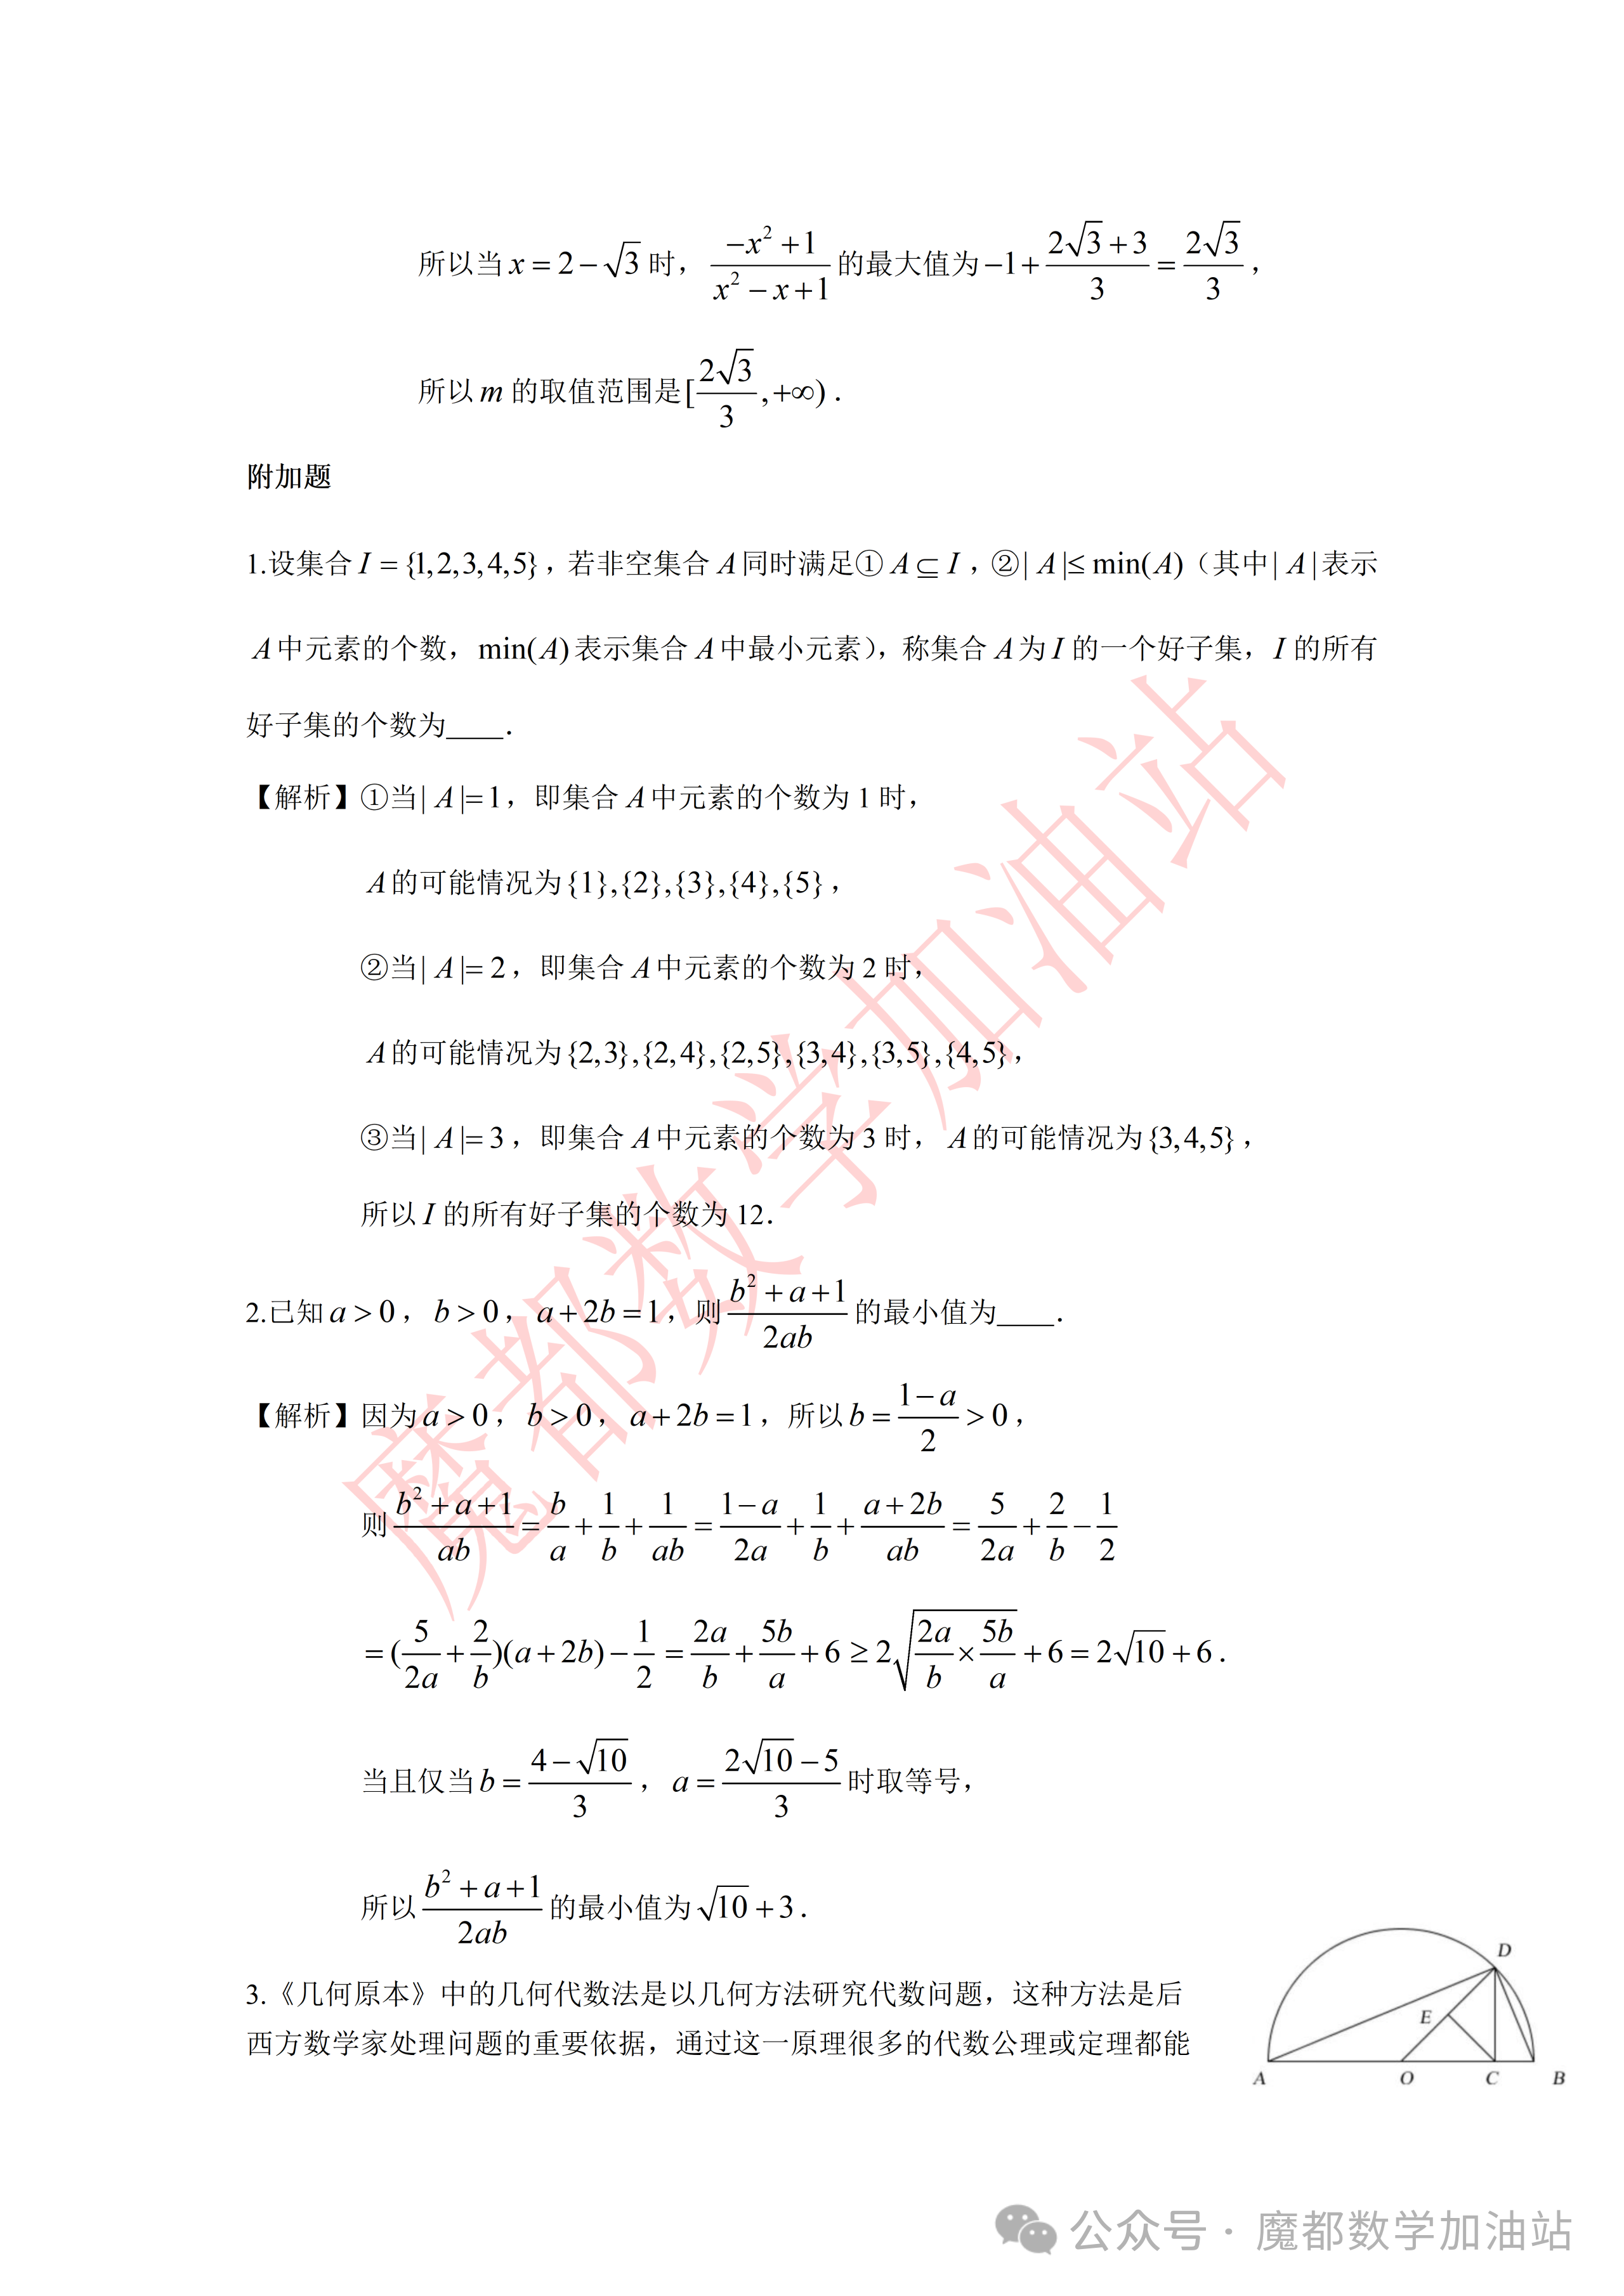
\includegraphics[width=.34\linewidth,trim=1960bp 310bp 90bp 3015bp,clip]{../原图/高一47_七宝中学_抱孩子练习9.26/08.png}
\end{center}

① $\dfrac{a+b}{2}\geqslant\sqrt{ab}$（$a>0$，$b>0$）；
② $a^2+b^2\geqslant2ab$（$a>0$，$b>0$）；
③ $\sqrt{ab}\geqslant\dfrac{2}{\dfrac1a+\dfrac1b}$（$a>0$，$b>0$）；
④ $\sqrt{\dfrac{a^2+b^2}{2}}\geqslant\dfrac{a+b}{2}$（$a>0$，$b>0$）.

\ifanswer
\solbegin
\step{因为 $AC+CB=a+b$，所以 $OD=\dfrac{AB}{2}=\dfrac{AC+CB}{2}=\dfrac{a+b}{2}$；}
\step{由射影定理得 $CD=\sqrt{AC\times CB}=\sqrt{ab}$，又因为 $OD\geqslant CD$，}
\step{所以 $\dfrac{a+b}{2}\geqslant\sqrt{ab}$，故①正确；}
\step{由射影定理得 $CD^2=DE\times OD$，所以 $DE=\dfrac{CD^2}{OD}=\dfrac{ab}{\dfrac{a+b}{2}}=\dfrac{2}{\dfrac1a+\dfrac1b}$，}
\step{又因为 $CD\geqslant DE$，所以 $\sqrt{ab}\geqslant\dfrac{2}{\dfrac1a+\dfrac1b}$，故③正确；}
\step{故该图形可以完成的所有无字证明为①③.}
\solend

\fi

% 注：原卷此处印作等式 $|x^2+a|+|x-a|=|x^2+x|$（在 $x>0$ 时与三角不等式下界等价），本稿曾改写成
% 不等式，现按原卷照录（原卷如此，照录未改）。
\item 若对任意 $x\in[2,3]$，均有 $|x^2+a|+|x-a|=|x^2+x|$，则实数 $a$ 的取值范围为 \blankline[4.4em].

\ifanswer
\solbegin
\step{因为 $|a|+|b|=|a+b|$ 当且仅当 $ab\geqslant0$ 时取等号，}
\step{所以 $(x^2+a)(x-a)\geqslant0$，即 $(a+x^2)(a-x)\leqslant0$，所以 $-x^2\leqslant a\leqslant x$ 恒成立，}
\step{因为 $x\in[2,3]$，所以 $-4\leqslant a\leqslant2$，所以实数 $a$ 的取值范围为 $[-4,2]$.}
\solend

\fi

\end{enumerate}

\end{document}
"
%
% 原始材料是微信公众号图文（公众号“魔都数学加油站”连载“27学年高一47”，署名“破晓”，
% 2026-10-02 17:56 发布，原文标题“27学年高一47——2026-2027年上海市七宝中学高一上抱孩子练习9.26”，
% 原文链接 https://mp.weixin.qq.com/s/mhkyDwjn7QFP_Z_NOcPkQA），正文为 9 张 PNG 页。
% 第 1—7、9 页分辨率为 4762×6735，第 8 页为 2560×3620；均按原图逐页核对。
% 原卷文字、选项、答案与解析均照录；粉色斜水印及灰色公众号页脚属水印/页脚，未录入。
%
% 卷首标题：原卷印作“2026-2027 年七宝中学高一上抱孩子练习 9.26”（公众号标题里的“上海市”
% 三字卷面标题行没有，本稿照卷面），年份区间按全稿惯例排 en dash，作业名保留原卷日期“9.26”。
% 原卷未印独立副标题；本稿按“知识模块”口径补出“集合与常用逻辑用语、不等式”。
%
% 与原卷的排版差异：
%   ① 原卷分“一、填空题”“二、选择题”“三、解答题”“附加题”四节；前三节题号为 3—16，
%      分别有 8 道填空、3 道选择、3 道解答；附加题另起 1—4 编号；
%   ② 原卷题下直接印答案/解析，本稿按全稿统一收进答案版；填空横线采用统一长度；
%   ③ 原卷未印副标题，本稿按“知识模块”口径补出（见卷首标题）；
%   ④ 全卷只有附加题第 3 题带图，直接从原卷第 8 页裁取。
%
% 原卷存疑（照录未改，见源码中该处上方注释）：
%   ① 第 9 题集合 C 的条件原文作“C={x|y=..., x 是整数}”，其中 y 未在集合描述中定义；
%      本稿照录原记号，未代换为 x。
%   ② 附加题第 3 题原文作“后西方数学家”，措辞存疑（疑漏“世”字）；本稿照录未改。
%
\documentclass[a4paper,11pt]{article}
\usepackage{common}

\begin{document}

\examtitlest[3]{2026--2027 年七宝中学高一上抱孩子练习 9.26}{集合与常用逻辑用语、不等式}

\bigsec{一、填空题}

\begin{enumerate}
\setcounter{enumi}{2}

\item 若不等式 $|x|<a$ 的一个充分条件为 $0<x<1$，则实数 $a$ 的取值范围是 \blankline[4.4em].

\ifanswer
\solbegin
\step{由 $|x|<a$ 得到 $-a<x<a$，}
\step{又不等式 $|x|<a$ 的一个充分条件为 $0<x<1$，所以 $a\geqslant1$.}
\solend

\fi

\item 已知命题“$\exists x\in\R$，使 $4x^2+(a-2)x+\dfrac14=0$”是假命题，则实数 $a$ 的取值范围是 \blankline[4.4em].

\ifanswer
\solbegin
% 注：原卷首句作“为真命题”（先按命题为真推出 $\Delta\geqslant0$，再由其为假得 $0<a<4$），原卷如此，照录未改。
\step{命题 $\exists x\in\R$，使 $4x^2+(a-2)x+\dfrac14=0$ 为真命题，}
\step{则 $\Delta=(a-2)^2-4\times4\times\dfrac14=a^2-4a\geqslant0$，解得 $a\leqslant0$ 或 $a\geqslant4$，}
\step{而命题“$\exists x\in\R$，使 $4x^2+(a-2)x+\dfrac14=0$”是假命题，则 $0<a<4$，}
\step{所以实数 $a$ 的取值范围是 $\{a\mid0<a<4\}$.}
\solend

\fi

\item 已知集合 $A=\{x\mid(a-1)x^2+3x-2=0\}$ 有且仅有两个子集，则实数 $a=$ \blankline[4.4em].

\ifanswer
\solbegin
\step{集合 $A=\{x\mid(a-1)x^2+3x-2=0\}$ 有且仅有两个不同的子集，}
\step{所以 $a-1=0$ 或 $\begin{cases}a-1\neq0\\\Delta=9+8(a-1)=0\end{cases}$，解得实数 $a=1$ 或 $a=-\dfrac18$.}
\solend

\fi

\item 已知函数 $y=x^2+bx+3$（其中 $b$ 是实数）中，$y$ 的取值范围是 $[0,+\infty)$，若关于 $x$ 的不等式 $x^2+bx+3<c$ 的解集为 $m-8<x<m$，则实数 $c$ 的值为 \blankline[4.4em].

\ifanswer
\solbegin
\step{因为 $y$ 的取值范围是 $[0,+\infty)$，所以 $\Delta=b^2-12=0$，解得 $b^2=12$，}
\step{因为不等式 $x^2+bx+3<c$ 的解集为 $m-8<x<m$，}
\step{令 $x^2+bx+3=c$，即 $x^2+bx+3-c=0$，方程的两根为 $x_1=m-8$，$x_2=m$，}
\step{所以 $|x_2-x_1|=\sqrt{(x_1+x_2)^2-4x_1x_2}=\sqrt{b^2-4(3-c)}=8$，即 $\sqrt{12-4(3-c)}=8$，}
\step{且判别式 $\Delta=b^2-4(3-c)=12-4(3-c)>0$，解得 $c=16$.}
\solend

\fi

\item 关于 $x$ 的不等式 $|x-1|+|x+1|\geqslant a$ 的解集为 $\R$，则实数 $a$ 的取值范围为 \blankline[4.4em].

\ifanswer
\solbegin
\step{因为 $|x-1|+|x+1|\geqslant|x-1-(x+1)|=2$，}
\step{若关于 $x$ 的不等式 $|x-1|+|x+1|\geqslant a$ 的解集为 $\R$，则实数 $a$ 的取值范围为 $a\leqslant2$.}
\solend

\fi

\item 已知 $m>0$，$xy>0$，当 $x+y=2$ 时，不等式 $\dfrac2x+\dfrac my\geqslant4$ 恒成立，则 $m$ 的取值范围是 \blankline[4.4em].

\ifanswer
\solbegin
\step{因为 $m>0$，$xy>0$，$x+y=2$，}
\step{所以 $\dfrac2x+\dfrac my=\dfrac12(x+y)\left(\dfrac2x+\dfrac my\right)
=\dfrac12\left(m+2+\dfrac{2y}{x}+\dfrac{mx}{y}\right)$}
\step{$\geqslant\dfrac12\left(m+2+2\sqrt{\dfrac{2y}{x}\cdot\dfrac{mx}{y}}\right)=\dfrac12\left(m+2+2\sqrt{2m}\right)$，}
\step{当且仅当 $\dfrac{2y}{x}=\dfrac{mx}{y}$，即 $y^2=\dfrac{mx^2}{2}$ 时取等号.}
\step{因为不等式 $\dfrac2x+\dfrac my\geqslant4$ 恒成立，所以 $\dfrac12(m+2+2\sqrt{2m})\geqslant4$，}
\step{整理得 $(\sqrt m+3\sqrt2)(\sqrt m-\sqrt2)\geqslant0$，解得 $\sqrt m\geqslant\sqrt2$，即 $m\geqslant2$，}
\step{所以 $m$ 的取值范围为 $[2,+\infty)$.}
\solend

\fi

\item 已知全集为 $\R$，集合 $D=\{x\mid x^2-ax+a^2-19=0\}$，
$B=\{y\mid y=-x^2+2x+2,\ y\text{ 是正整数}\}$，
% 注：本题集合 C 的条件原文作“C={x|y=..., x 是整数}”，其中 y 未在集合描述中定义；照录未改。
集合 $C=\left\{x\mathrel{\Big|}y=\sqrt{\dfrac{2-x}{x+1}},\ x\text{ 是整数}\right\}$，且集合 $D$ 满足 $D\cap B\neq\varnothing$，$\overline{D}\cup\overline{C}=\R$，则实数 $a$ 的值是 \blankline[4.4em].

\ifanswer
\solbegin
\step{集合 $B=\{y\mid y=-x^2+2x+2,\ y\text{ 是正整数}\}=\{1,2,3\}$，}
\step{集合 $C=\left\{x\mathrel{\Big|}y=\sqrt{\dfrac{2-x}{x+1}},\ x\text{ 是整数}\right\}=\{0,1,2\}$，}
\step{集合 $D=\{x\mid x^2-ax+a^2-19=0\}$ 且集合 $D$ 满足 $D\cap B\neq\varnothing$，$\overline{D}\cup\overline{C}=\R$，}
\step{所以 $3\in D$，解得 $a=5$ 或 $a=-2$，}
\step{经检验，$a=5$ 不符合 $\overline{D}\cup\overline{C}=\R$，舍去，$a=-2$ 满足题意，即 $a=-2$.}
\solend

\fi

% 注：本题解析中，$a=\pm2\sqrt2$ 时 $B$ 的二重根按 $-\dfrac a2$ 应为 $\mp\sqrt2$，原卷印作 $\mp2\sqrt2$、
% $-\dfrac{3\sqrt2}4$，$C(B)=3$ 的计算也随之按原卷保留（原卷如此，照录未改）。
\item 用 $C(A)$ 表示非空集合 $A$ 中的元素的个数，定义 $A*B=|C(A)-C(B)|$，已知集合 $A$ 有三个真子集，
$B=\{x\mid(ax^2+3x)(x^2+ax+2)=0,\ x\in\R\}$，若 $A*B=1$，设实数 $a$ 所有可能取值构成集合 $S$，则 $C(S)=$ \blankline[4.4em].

\ifanswer
\solbegin
\step{集合 $A$ 有三个真子集，则集合 $A$ 中有 $2$ 个元素，则 $C(A)=2$，}
\step{由 $A*B=1$，得 $C(B)=1$ 或 $3$，}
\step{即方程 $(ax^2+3x)\cdot(x^2+ax+2)=0$ 有一个根或 $3$ 个根；}
\step{若 $(ax^2+3x)\cdot(x^2+ax+2)=0$，则必有 $ax^2+3x=0$ 或 $x^2+ax+2=0$，}
\step{若 $ax^2+3x=0$，则 $x=0$ 或 $ax+3=0$，}
\step{当 $a=0$ 时，$B=\{0\}$，$C(B)=1$，符合题意；}
\step{当 $a\neq0$ 时，$ax^2+3x=0$ 对应的根为 $0$ 和 $-\dfrac3a$；}
\step{故①需 $x^2+ax+2=0$ 有两等根且根不为 $0$ 和 $-\dfrac3a$，}
\step{当 $\Delta=0$ 时，$a=\pm2\sqrt2$，}
\step{$a=2\sqrt2$，此时 $B=\left\{0,-2\sqrt2,-\dfrac{3\sqrt2}{4}\right\}$，$C(B)=3$，符合题意；}
\step{$a=-2\sqrt2$，此时 $B=\left\{0,2\sqrt2,\dfrac{3\sqrt2}{4}\right\}$，$C(B)=3$，符合题意；}
\step{②当 $-\dfrac3a$ 是 $x^2+ax+2=0$ 的根时，解得 $a=\pm3$；}
\step{$a=3$，此时 $B=\{0,-1,-2\}$，$C(B)=3$，符合题意；}
\step{$a=-3$，此时 $B=\{0,1,2\}$，$C(B)=3$，符合题意；}
\step{综上，$a$ 可取的值为 $0$、$\pm3$、$\pm2\sqrt2$，则 $C(S)=5$.}
\solend

\fi

\end{enumerate}

\bigsec{二、选择题}

\begin{enumerate}
\setcounter{enumi}{10}

\item 已知集合 $A=\left\{x\mathrel{\Big|}\dfrac1x<1\right\}$，$B=\{x\mid x^2-2x-3\leqslant0\}$，则 $A\cap B=$\mbox{（\quad）}

\keepwithprev
A. $\{x\mid1<x\leqslant3\}$\qquad B. $\{x\mid1\leqslant x\leqslant3\text{ 或 }-1\leqslant x<0\}$

C. $\{x\mid-1\leqslant x<0\}$\qquad D. $\{x\mid1<x\leqslant3\text{ 或 }-1\leqslant x<0\}$

\ans{$D$}

% 注：原卷本题只有题干＋选项（答案印在括号内），没有解析；此处照录原卷的"无解析"状态，不排解析。
\item 使 $x(y-2)=0$ 成立的一个充分条件是\mbox{（\quad）}

\keepwithprev
A. $x^2+(y-2)^2=0$\qquad B. $(x-2)^2+y^2=0$

C. $x^2+y^2=1$\qquad D. $x+y-2=0$

\ans{$A$}

\ifanswer
\solbegin
\step{对于 $A$：若 $x^2+(y-2)^2=0$，则 $x=0$ 且 $y=2$，此时 $x(y-2)=0$ 成立，}
\step{即充分性成立.}
\step{若 $x(y-2)=0$，则 $x=0$ 或 $y=2$，当 $x=0$，$y=3$ 时，$x^2+(y-2)^2=0$ 不成立，}
\step{即必要性不成立，}
\step{故 $x^2+(y-2)^2=0$ 是 $x(y-2)=0$ 成立的充分不必要条件；}
\step{对于 $B$：$(x-2)^2+y^2=0$，则 $x=2$ 且 $y=0$，此时 $x(y-2)=0$ 不成立，}
\step{即充分性不成立；}
\step{对于 $C$：$x^2+y^2=1$，此时 $x(y-2)=0$ 不一定成立，即充分性不成立；}
\step{对于 $D$：$x+y-2=0$，此时 $x(y-2)=0$ 不一定成立，即充分性不成立.}
\step{故选 $A$.}
\solend

\fi

\item 已知 $a$、$b$、$c\in\R$，若关于 $x$ 的不等式 $0\leqslant x+\dfrac ax+b\leqslant\dfrac cx-1$ 的解集为 $[x_1,x_2]\cup\{x_3\}$（$x_3>x_2>x_1>0$），则\mbox{（\quad）}

\keepwithprev
A. 不存在有序数组 $(a,b,c)$，使得 $x_2-x_1=1$

B. 存在唯一有序数组 $(a,b,c)$，使得 $x_2-x_1=1$

C. 有且只有两组有序数组 $(a,b,c)$，使得 $x_2-x_1=1$

D. 存在无穷多组有序数组 $(a,b,c)$，使得 $x_2-x_1=1$

\ans{$D$}

\ifanswer
\solbegin
\step{因为不等式 $0\leqslant x+\dfrac ax+b\leqslant\dfrac cx-1$ 的解集为 $[x_1,x_2]\cup\{x_3\}$（$x_3>x_2>x_1>0$），}
\step{所以 $0\leqslant x^2+bx+a\leqslant c-x$ 在 $[x_1,x_2]\cup\{x_3\}$ 上成立，}
\step{假设 $x_1=m$，$x_2=m+1$，$x_3=n$，}
\step{则 $c-n=0=n^2+bn+a$，由 $x_3$ 为一个独立的数得出，}
\step{所以 $n=c$，且 $m+1$ 与 $n$ 为方程 $x^2+bx+a=0$ 的两个根，}
\step{因为 $x_3>x_2>x_1>0$，所以 $-b=m+n+1=m+c+1$，$a=mn+n=mc+c$，}
\step{所以 $b=-m-c-1$，}
\step{且点 $(x_1,x_1^2+bx_1+a)$ 为 $y=x^2+bx+a$ 与 $y=c-x$ 的左交点，}
\step{所以 $m^2+bm+a=c-m$ 且 $b=-m-c-1$，$a=mc+c$，}
% 注：原卷此行的末句作“所以 $c-m=c-m$ 恒成立”（未写成 $x_2-x_1=1$），原卷如此，照录未改。
\step{故 $m^2+bm+a=m^2-m^2-mc-m+mc+c=c-m$，所以 $c-m=c-m$ 恒成立，}
\step{所以不论 $a$、$b$、$c$ 取何值，$x_2-x_1=1$ 恒成立，}
\step{即存在无穷多组有序数组 $(a,b,c)$，使得 $x_2-x_1=1$，}
\step{故选项 $A$、$B$、$C$ 错误，选项 $D$ 正确. 故选 $D$.}
\solend

\fi

\end{enumerate}

\bigsec{三、解答题}

\begin{enumerate}
\setcounter{enumi}{13}

\item 设正实数 $x$、$y$，满足 $2x+y=1$，求：

\begin{enumerate}[label=(\arabic*)]
\item $\sqrt{2x}+\sqrt y$ 的最大值；
\item $\dfrac2x+\dfrac1y$ 的最小值.
\end{enumerate}

\ifanswer
\solbegin
\stepm{(1)}{对于 $(\sqrt{2x}+\sqrt y)^2=2x+y+2\sqrt{2xy}\leqslant1+1=2$，}
\step{当且仅当 $\sqrt{2x}=\sqrt y$ 时取等号，故 $\sqrt{2x}+\sqrt y$ 的最大值为 $\sqrt2$；}
\stepm{(2)}{$\dfrac2x+\dfrac1y=\left(\dfrac2x+\dfrac1y\right)(2x+y)=5+\dfrac{2y}{x}+\dfrac{2x}{y}\geqslant5+4=9$，}
\step{当且仅当 $\dfrac{2y}{x}=\dfrac{2x}{y}$，即 $x=y=\dfrac13$ 时取等号，故 $\dfrac2x+\dfrac1y$ 的最小值为 $9$.}
\solend

\fi

\ansspace[6]

\item 设 $x_1$、$x_2$ 为关于 $x$ 的方程 $x^2-2(m+2)x+m^2-1=0$ 的两实数根.

\begin{enumerate}[label=(\arabic*)]
\item 若 $x_1$、$x_2$ 满足 $x_1^2+x_2^2=18$，试求 $m$ 的值；
\item 若 $x_1$、$x_2$ 均大于 $0$，求 $m$ 的取值范围.
\end{enumerate}

\ifanswer
\solbegin
\stepm{(1)}{由 $\Delta=4(m+2)^2-4(m^2-1)\geqslant0$，解得 $m\geqslant-\dfrac54$，}
\step{由韦达定理得 $x_1+x_2=2(m+2)$，$x_1x_2=m^2-1$，}
\step{又 $x_1^2+x_2^2=(x_1+x_2)^2-2x_1x_2=4(m+2)^2-2(m^2-1)=18$，}
\step{即 $m^2+8m=0$，解得 $m=0$ 或 $m=-8$（舍），故 $m$ 的值为 $0$；}
% 注：原卷此处作“由（2）得”（对照上一小问，所指应为（1）），原卷如此，照录未改。
\stepm{(2)}{由（2）得 $m\geqslant-\dfrac54$，}
\step{又 $x_1$、$x_2$ 均大于 $0$，则 $\begin{cases}2(m+2)>0\\m^2-1>0\end{cases}$，解得 $\begin{cases}m>-2\\m>1\text{或}m<-1\end{cases}$，}
\step{综上，实数 $m$ 的取值范围为 $\left[-\dfrac54,-1\right)\cup(1,+\infty)$.}
\solend

\fi

\ansspace[6]

\item 已知函数 $f(x)=(m+1)x^2-mx+m-1$（$m\in\R$）.

\begin{enumerate}[label=(\arabic*)]
\item 若不等式 $f(x)<0$ 的解集是空集，求 $m$ 的取值范围；
\item 当 $m>-2$ 时，解不等式 $f(x)\geqslant m$；
\item 若不等式 $f(x)\geqslant0$ 的解集为 $D$，若 $[-1,1]\subseteq D$，求 $m$ 的取值范围.
\end{enumerate}

\ifanswer
\solbegin
\stepm{(1)}{①当 $m+1=0$，即 $m=-1$ 时，$f(x)=x-2$，不合题意；}
\step{②当 $m+1\neq0$，即 $m\neq-1$ 时，$\begin{cases}m+1>0\\\Delta=m^2-4(m+1)(m-1)\leqslant0\end{cases}$，解得 $m\geqslant\dfrac{2\sqrt3}{3}$，}
\step{所以 $m$ 的取值范围是 $\left[\dfrac{2\sqrt3}{3},+\infty\right)$；}
\stepm{(2)}{因为 $f(x)\geqslant m$，所以 $(m+1)x^2-mx-1\geqslant0$，即 $[(m+1)x+1](x-1)\geqslant0$，}
\step{①当 $m+1=0$ 即 $m=-1$ 时，不等式的解集为 $[1,+\infty)$；}
\step{②当 $m+1>0$ 即 $m>-1$ 时，$\left(x+\dfrac1{m+1}\right)(x-1)\geqslant0$，}
\step{因为 $-\dfrac1{m+1}<0$，所以不等式的解集为 $\left(-\infty,-\dfrac1{m+1}\right]\cup[1,+\infty)$；}
\step{③当 $m+1<0$ 即 $-2<m<-1$ 时，$\left(x+\dfrac1{m+1}\right)(x-1)\leqslant0$，}
\step{因为 $-2<m<-1$，所以 $-1<m+1<0$，所以 $-\dfrac1{m+1}>1$，}
\step{所以不等式的解集为 $\left[1,-\dfrac1{m+1}\right]$；}
\stepm{(3)}{不等式 $f(x)\geqslant0$ 的解集为 $D$，若 $[-1,1]\subseteq D$，}
\step{即对任意的 $x\in[-1,1]$，不等式 $(m+1)x^2-mx+m-1\geqslant0$ 恒成立，}
\step{即 $m(x^2-x+1)\geqslant-x^2+1$ 恒成立，}
\step{因为 $x^2-x+1>0$ 恒成立，所以 $m\geqslant\dfrac{-x^2+1}{x^2-x+1}=-1+\dfrac{2-x}{x^2-x+1}$ 恒成立，}
\step{设 $t=2-x$，则 $t\in[1,3]$，$x=2-t$，}
\step{则 $\dfrac{2-x}{x^2-x+1}=\dfrac{t}{(2-t)^2-(2-t)+1}=\dfrac{t}{t^2-3t+3}=\dfrac1{t+\dfrac3t-3}$，}
\step{因为 $t+\dfrac3t\geqslant2\sqrt3$，当且仅当 $t=\sqrt3$ 时取等号，}
\step{所以 $\dfrac{2-x}{x^2-x+1}\leqslant\dfrac1{2\sqrt3-3}=\dfrac{2\sqrt3+3}{3}$，当且仅当 $x=2-\sqrt3$ 时取等号，}
\step{所以当 $x=2-\sqrt3$ 时，$\dfrac{-x^2+1}{x^2-x+1}$ 的最大值为 $-1+\dfrac{2\sqrt3+3}{3}=\dfrac{2\sqrt3}{3}$，}
\step{所以 $m$ 的取值范围是 $\left[\dfrac{2\sqrt3}{3},+\infty\right)$.}
\solend

\fi

\ansspace[8]

\end{enumerate}

\bigsec{附加题}

\begin{enumerate}

\item 设集合 $I=\{1,2,3,4,5\}$，若非空集合 $A$ 同时满足① $A\subseteq I$，② $|A|\leqslant\min(A)$（其中 $|A|$ 表示集合 $A$ 中元素的个数，$\min(A)$ 表示集合 $A$ 中最小元素），称集合 $A$ 为 $I$ 的一个好子集，$I$ 所有好子集的个数为 \blankline[4.4em].

\ifanswer
\solbegin
\step{①当 $|A|=1$，即集合 $A$ 中元素的个数为 $1$ 时，}
\step{$A$ 的可能情况为 $\{1\}$、$\{2\}$、$\{3\}$、$\{4\}$、$\{5\}$，}
\step{②当 $|A|=2$，即集合 $A$ 中元素的个数为 $2$ 时，}
\step{$A$ 的可能情况为 $\{2,3\}$、$\{2,4\}$、$\{2,5\}$、$\{3,4\}$、$\{3,5\}$、$\{4,5\}$，}
\step{③当 $|A|=3$，即集合 $A$ 中元素的个数为 $3$ 时，$A$ 的可能情况为 $\{3,4,5\}$，}
\step{所以 $I$ 的所有好子集的个数为 $12$.}
\solend

\fi

\item 已知 $a>0$，$b>0$，$a+2b=1$，则 $\dfrac{b^2+a+1}{2ab}$ 的最小值为 \blankline[4.4em].

\ifanswer
\solbegin
\step{因为 $a>0$，$b>0$，$a+2b=1$，所以 $b=\dfrac{1-a}{2}>0$，}
\step{则 $\dfrac{b^2+a+1}{ab}=\dfrac ba+\dfrac1b+\dfrac1{ab}=\dfrac{1-a}{2a}+\dfrac1b+\dfrac{a+2b}{ab}=\dfrac5{2a}+\dfrac2b-\dfrac12$}
\step{$=\left(\dfrac5{2a}+\dfrac2b\right)(a+2b)-\dfrac12=\dfrac{2a}{b}+\dfrac{5b}{a}+6\geqslant2\sqrt{\dfrac{2a}{b}\times\dfrac{5b}{a}}+6=2\sqrt{10}+6$.}
\step{当且仅当 $b=\dfrac{4-\sqrt{10}}{3}$，$a=\dfrac{2\sqrt{10}-5}{3}$ 时取等号，}
\step{所以 $\dfrac{b^2+a+1}{2ab}$ 的最小值为 $\sqrt{10}+3$.}
\solend

\fi

% 注：本题原文作“后西方数学家”，措辞存疑（疑漏“世”字）；照录未改，见文件头“原卷存疑”②。
% 又原文作"很多的代数公理或定理都能够通过图形实现证明"（"公理"疑为"公式"笔误）、
% "连结 OD,AD,BD"，均原卷如此，照录未改。
\item 《几何原本》中的几何代数法是以几何方法研究代数问题，这种方法是后西方数学家处理问题的重要依据，通过这一原理很多的代数公理或定理都能够通过图形实现证明，也称之为无字证明，现有图形如图所示，$C$ 为线段 $AB$ 上的点，且 $AC=a$，$BC=b$，$O$ 为 $AB$ 的中点，以 $AB$ 为直径作半圆，过点 $C$ 作 $AB$ 的垂线交半圆于 $D$，连结 $OD,AD,BD$，过点 $C$ 作 $OD$ 的垂线，垂足为 $E$，若不添加辅助线，则该图形可以完成的所有无字证明为 \blankline[4.4em]（填写序号）.

\begin{center}
% 插图直接裁自原卷第 8 页，未重绘；用 trim/clip 保留原图与标注。
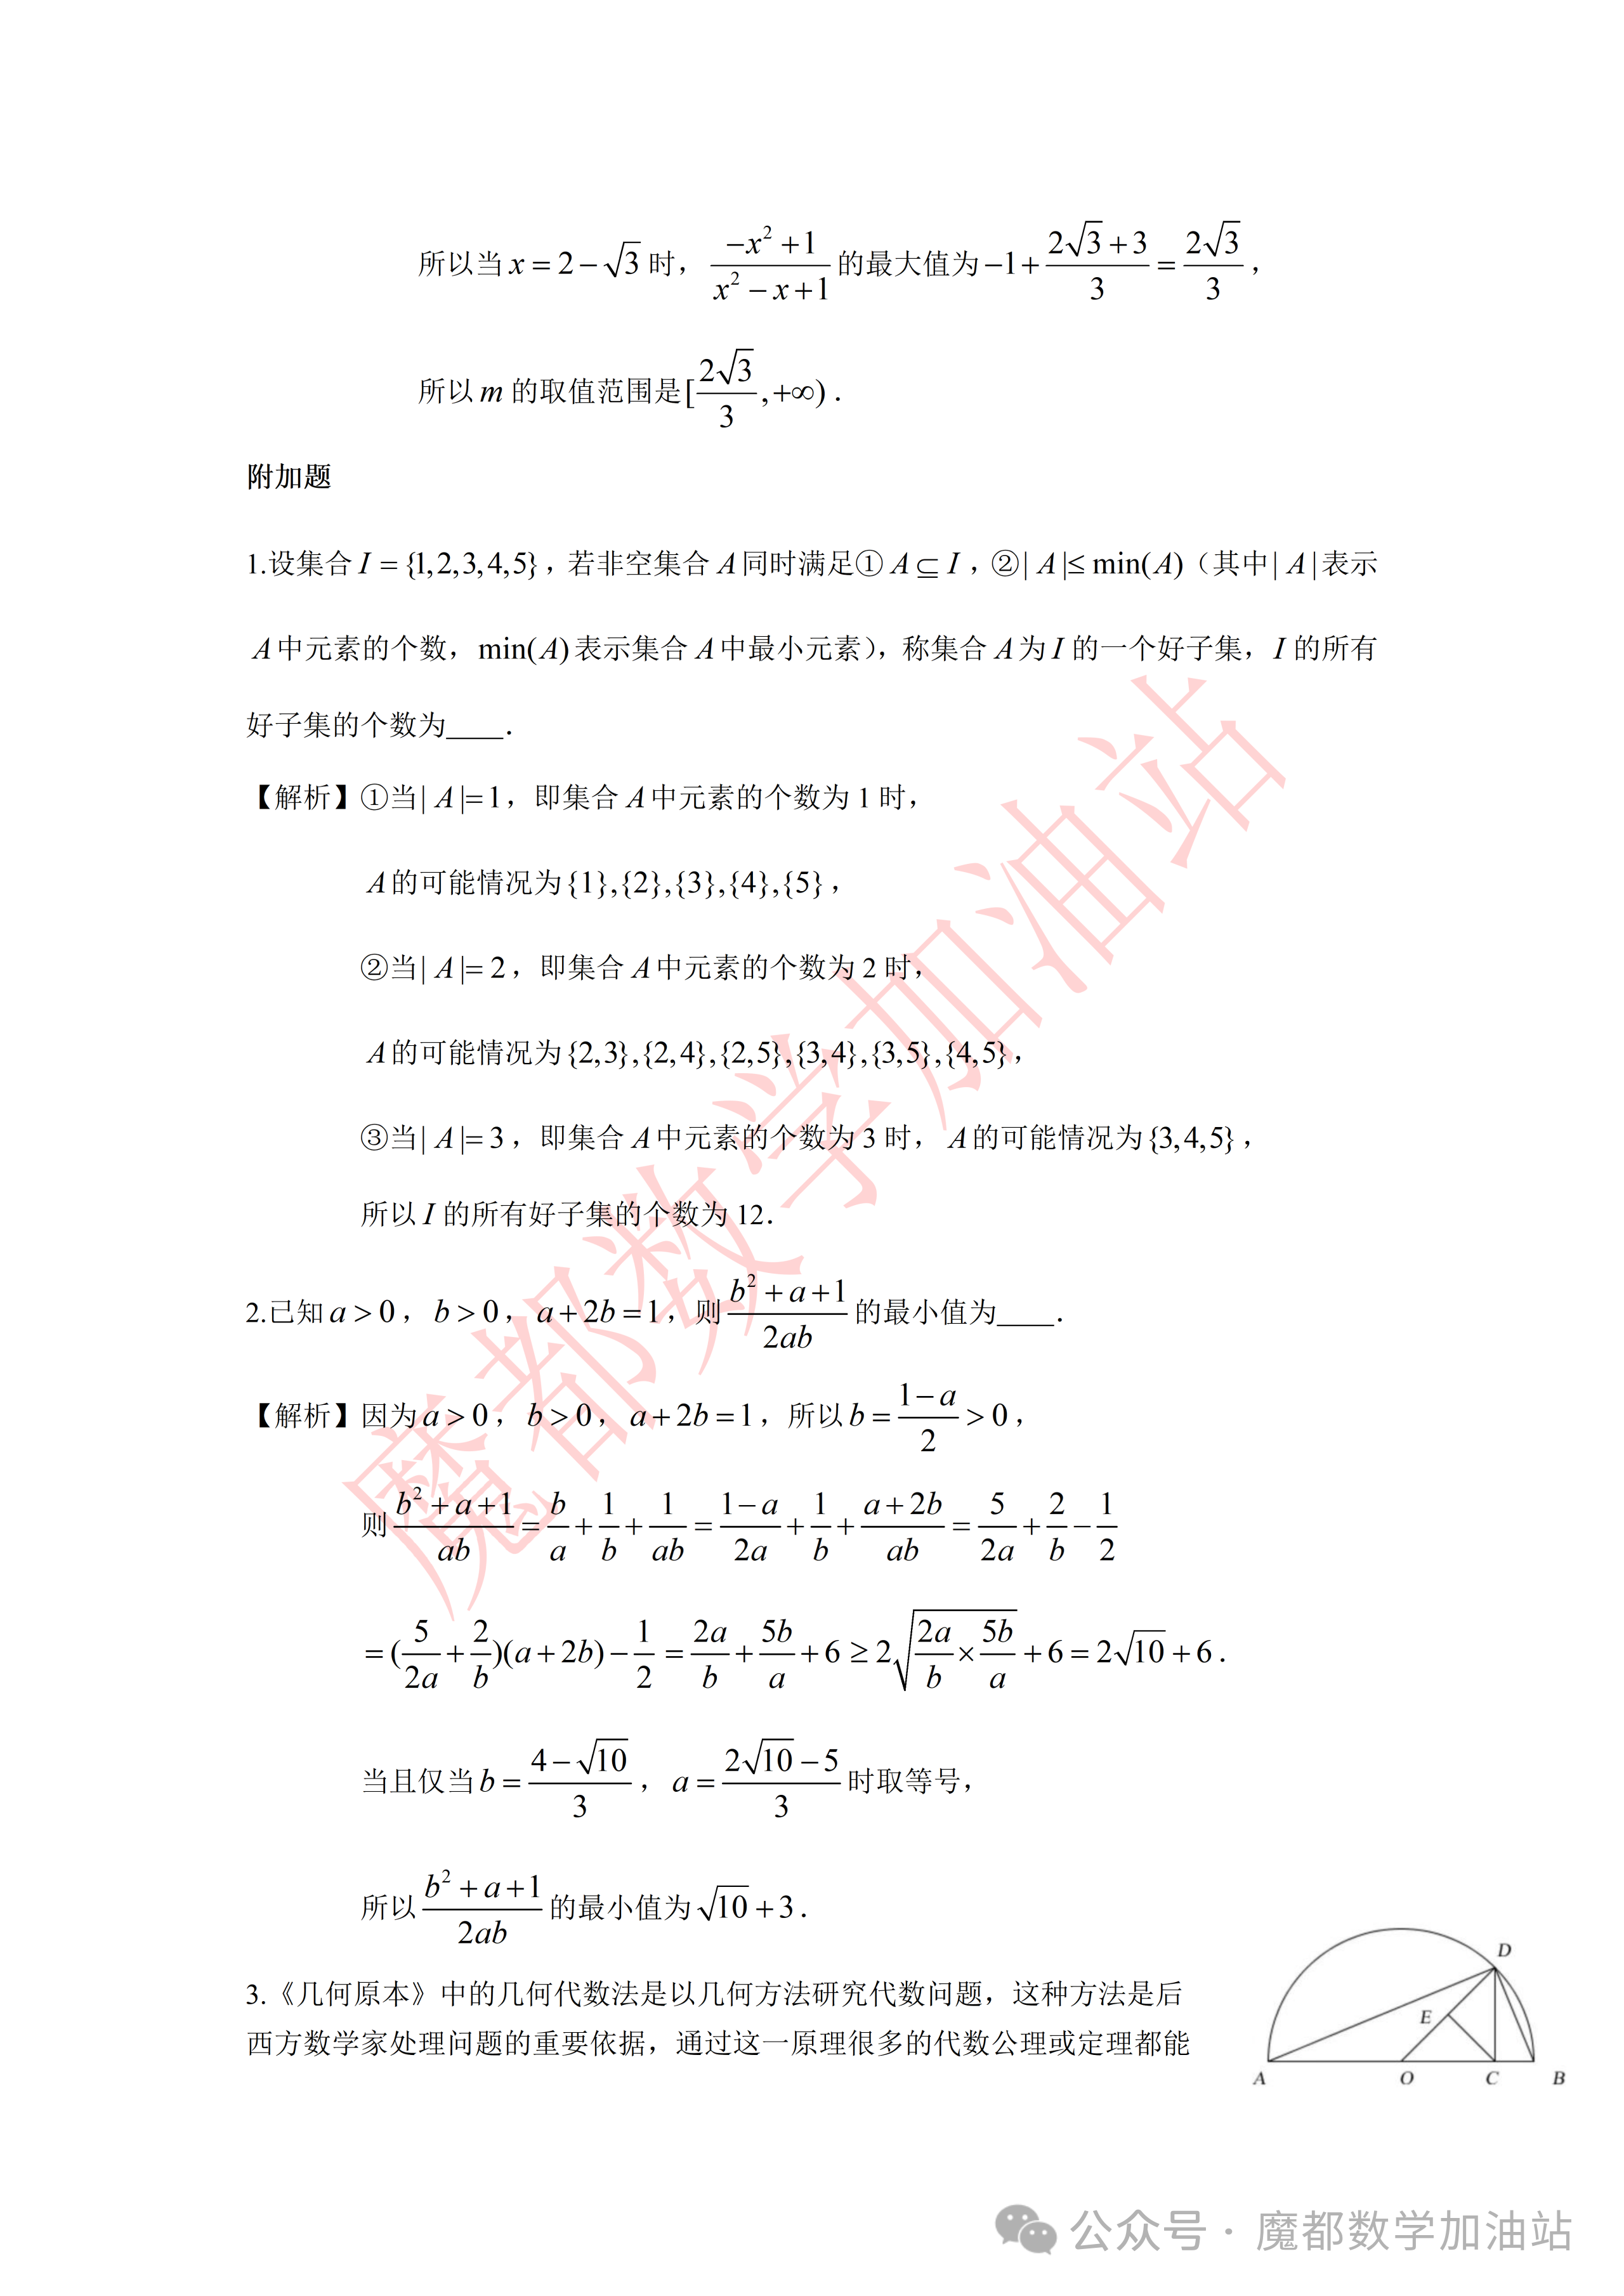
\includegraphics[width=.34\linewidth,trim=1960bp 310bp 90bp 3015bp,clip]{../原图/高一47_七宝中学_抱孩子练习9.26/08.png}
\end{center}

① $\dfrac{a+b}{2}\geqslant\sqrt{ab}$（$a>0$，$b>0$）；
② $a^2+b^2\geqslant2ab$（$a>0$，$b>0$）；
③ $\sqrt{ab}\geqslant\dfrac{2}{\dfrac1a+\dfrac1b}$（$a>0$，$b>0$）；
④ $\sqrt{\dfrac{a^2+b^2}{2}}\geqslant\dfrac{a+b}{2}$（$a>0$，$b>0$）.

\ifanswer
\solbegin
\step{因为 $AC+CB=a+b$，所以 $OD=\dfrac{AB}{2}=\dfrac{AC+CB}{2}=\dfrac{a+b}{2}$；}
\step{由射影定理得 $CD=\sqrt{AC\times CB}=\sqrt{ab}$，又因为 $OD\geqslant CD$，}
\step{所以 $\dfrac{a+b}{2}\geqslant\sqrt{ab}$，故①正确；}
\step{由射影定理得 $CD^2=DE\times OD$，所以 $DE=\dfrac{CD^2}{OD}=\dfrac{ab}{\dfrac{a+b}{2}}=\dfrac{2}{\dfrac1a+\dfrac1b}$，}
\step{又因为 $CD\geqslant DE$，所以 $\sqrt{ab}\geqslant\dfrac{2}{\dfrac1a+\dfrac1b}$，故③正确；}
\step{故该图形可以完成的所有无字证明为①③.}
\solend

\fi

% 注：原卷此处印作等式 $|x^2+a|+|x-a|=|x^2+x|$（在 $x>0$ 时与三角不等式下界等价），本稿曾改写成
% 不等式，现按原卷照录（原卷如此，照录未改）。
\item 若对任意 $x\in[2,3]$，均有 $|x^2+a|+|x-a|=|x^2+x|$，则实数 $a$ 的取值范围为 \blankline[4.4em].

\ifanswer
\solbegin
\step{因为 $|a|+|b|=|a+b|$ 当且仅当 $ab\geqslant0$ 时取等号，}
\step{所以 $(x^2+a)(x-a)\geqslant0$，即 $(a+x^2)(a-x)\leqslant0$，所以 $-x^2\leqslant a\leqslant x$ 恒成立，}
\step{因为 $x\in[2,3]$，所以 $-4\leqslant a\leqslant2$，所以实数 $a$ 的取值范围为 $[-4,2]$.}
\solend

\fi

\end{enumerate}

\end{document}
